\usepackage{geometry}
\usepackage{fontspec}
\usepackage{booktabs}
\usepackage{longtable}
\usepackage{siunitx}
\usepackage{framed}
\usepackage{multirow}
\usepackage[table]{xcolor}
 \definecolor{shadecolor}{RGB}{248,248,248}
\usepackage{grffile}
\usepackage{graphicx}
\usepackage{morefloats}
\usepackage[bf,singlelinecheck=on]{caption}
\usepackage{parskip}
 \setlength{\parindent}{15pt}
 % should be last package call in the preamble (?)
 \usepackage{hyperref}
  \urlstyle{same}

%\renewcommand{\textfraction}{0.05}
%\renewcommand{\topfraction}{0.8}
%\renewcommand{\bottomfraction}{0.8}
%\renewcommand{\floatpagefraction}{0.75}

\renewenvironment{quote}{\begin{VF}}{\end{VF}}
\let\oldhref\href
\renewcommand{\href}[2]{#2\footnote{\url{#1}}}

\ifxetex
  \usepackage{letltxmacro}
  \setlength{\XeTeXLinkMargin}{1pt}
  \LetLtxMacro\SavedIncludeGraphics\includegraphics
  \def\includegraphics#1#{% #1 catches optional stuff (star/opt. arg.)
    \IncludeGraphicsAux{#1}%
  }%
  \newcommand*{\IncludeGraphicsAux}[2]{%
    \XeTeXLinkBox{%
      \SavedIncludeGraphics#1{#2}%
    }%
  }%
\fi

\makeatletter
\newenvironment{kframe}{%
\medskip{}
\setlength{\fboxsep}{.8em}
 \def\at@end@of@kframe{}%
 \ifinner\ifhmode%
  \def\at@end@of@kframe{\end{minipage}}%
  \begin{minipage}{\columnwidth}%
 \fi\fi%
 \def\FrameCommand##1{\hskip\@totalleftmargin \hskip-\fboxsep
 \colorbox{shadecolor}{##1}\hskip-\fboxsep
     % There is no \\@totalrightmargin, so:
     \hskip-\linewidth \hskip-\@totalleftmargin \hskip\columnwidth}%
 \MakeFramed {\advance\hsize-\width
   \@totalleftmargin\z@ \linewidth\hsize
   \@setminipage}}%
 {\par\unskip\endMakeFramed%
 \at@end@of@kframe}
\makeatother

\newenvironment{Shaded}{\begin{kframe}}{\end{kframe}}

\newenvironment{rmdblock}[1]
  {
  \begin{itemize}
  \renewcommand{\labelitemi}{
    \raisebox{-.7\height}[0pt][0pt]{
      {\setkeys{Gin}{width=3em,keepaspectratio}\includegraphics{images/#1}}
    }
  }
  \setlength{\fboxsep}{1em}
  \begin{kframe}
  \item
  }
  {
  \end{kframe}
  \end{itemize}
  }

\newenvironment{rmdnote}
  {\begin{rmdblock}{note}}
  {\end{rmdblock}}

\newenvironment{rmdcaution}
  {\begin{rmdblock}{caution}}
  {\end{rmdblock}}

\newenvironment{rmdimportant}
  {\begin{rmdblock}{important}}
  {\end{rmdblock}}

\newenvironment{rmdtip}
  {\begin{rmdblock}{tip}}
  {\end{rmdblock}}

\newenvironment{rmdwarning}
  {\begin{rmdblock}{warning}}
  {\end{rmdblock}}

%\usepackage{makeidx}
% \makeindex

\usepackage{amsthm}
\makeatletter
\def\thm@space@setup{%
  \thm@preskip=8pt plus 2pt minus 4pt
  \thm@postskip=\thm@preskip
}
\makeatother

\begin{document}


\frontmatter

%include the cover as title page and set the page counter to -1 in order to start with the title page as 1 (i)
\setcounter{page}{-1}\includepdf[pages={1}]{neuroanatomy_text_dark_cover.pdf}


\maketitle

\setcounter{tocdepth}{1}
\tableofcontents

%insert empty page
\clearpage

\listoftables
\listoffigures


\hypertarget{acknowledgements}{%
\chapter*{Acknowledgements}\label{acknowledgements}}
\addcontentsline{toc}{chapter}{Acknowledgements}

The creation of this text was greatly facilitated and owes a major debt to \href{https://www.wikipedia.org}{Wikipedia} and its large number of voluntary contributors. I very liberally copied from many Wikipedia pages and then remixed, edited, adapted and added text. With your continued support and help this book can only get better over time. I urge you to email me with your criticisms and suggestions at \href{mailto:nsucher@salemstate.mass.edu}{\nolinkurl{nsucher@salemstate.mass.edu}}. This book is made available as an open educational resource under \href{https://creativecommons.org/licenses/by-sa/3.0/deed.en}{Creative Commons Attribution-Share Alike 3.0 Unported} United States License for others to do as I did and improve and adapt to specific requirements. I am grateful for the support provided by the \href{}{Salem State University's OER initiative}.

\mainmatter
\hypertarget{the-nervous-system}{%
\chapter{The Nervous System}\label{the-nervous-system}}

\hypertarget{introduction}{%
\section{Introduction}\label{introduction}}

The nervous system is a highly complex part of an animal that coordinates its actions and sensory information by transmitting signals to and from different parts of its body. The nervous system detects environmental changes that impact the body, then works in tandem with the endocrine system to respond to such events.



\begin{figure}

{\centering 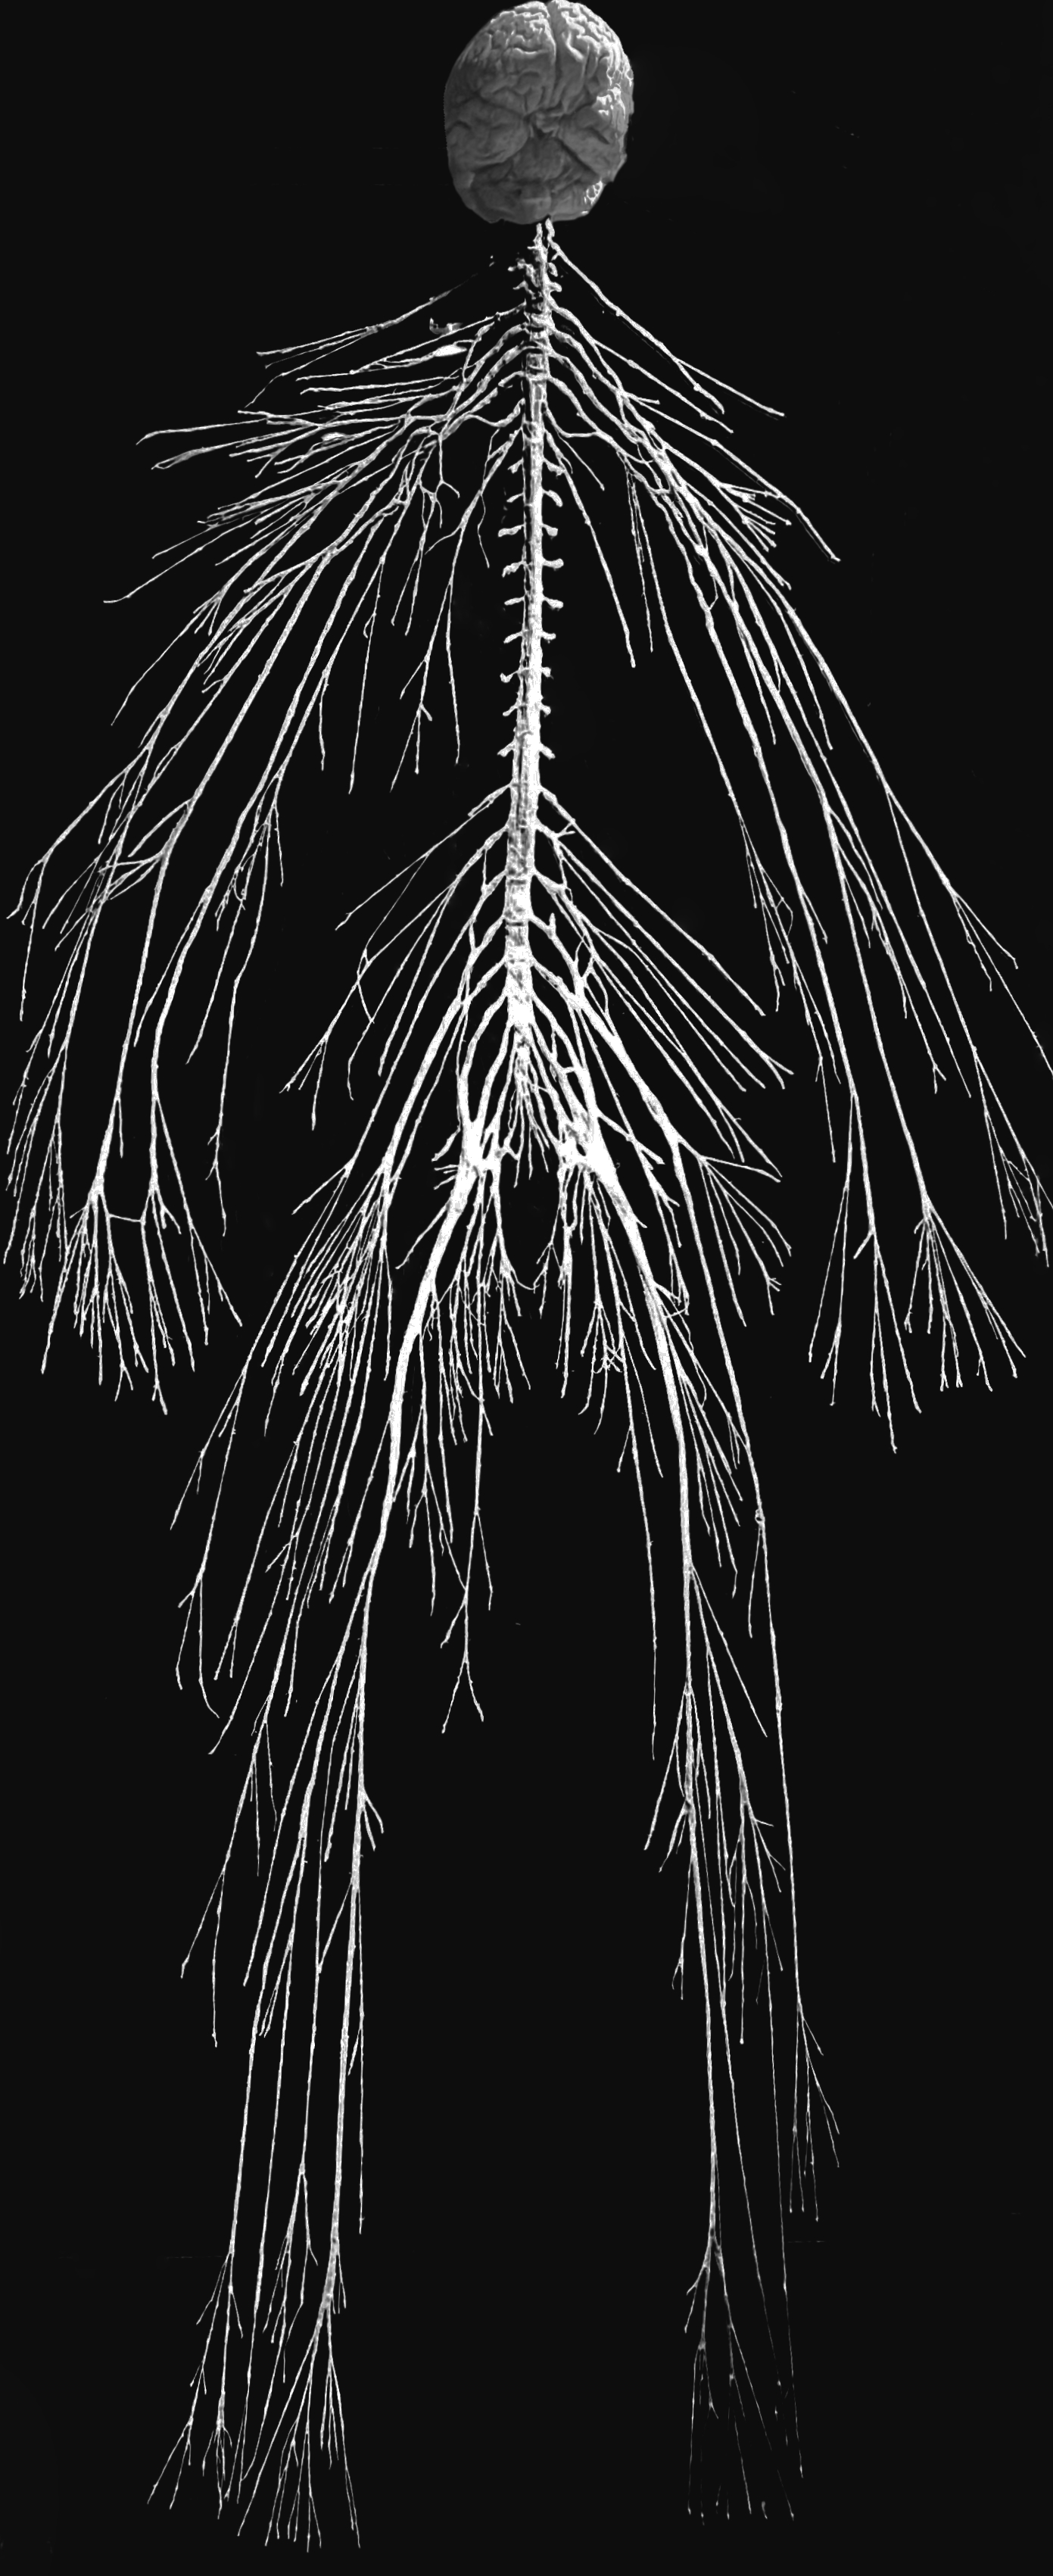
\includegraphics[width=0.7\linewidth]{./figures/nervoussystem/NervousSystem} 

}

\caption{The human nervous system.}\label{fig:nervoussystem}
\end{figure}

The nervous system derives its name from nerves, which are cylindrical bundles of fibers (the axons of neurons), that emanate from the brain and spinal cord, and branch repeatedly to innervate every part of the body. Nerves are large enough to have been recognized by the ancient Egyptians, Greeks, and Romans, but their internal structure was not understood until it became possible to examine them using a microscope.



\begin{figure}

{\centering 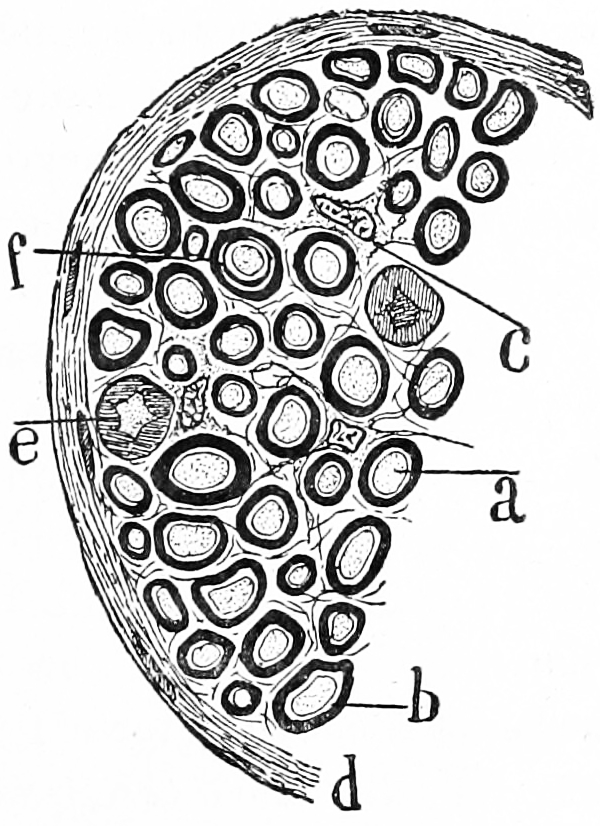
\includegraphics[width=0.7\linewidth]{./figures/nervoussystem/CajalNerve} 

}

\caption{Transverse section of a nerve. a) a single nerve fibre (axon) surrounded by a thick layer of myelin. c) an interstitial cell. \href{https://wellcomelibrary.org/item/b2129592x\#?c=0\&m=0\&s=0\&cv=14\&z=0\%2C-3.48\%2C1\%2C8.6591}{Histologie du système nerveux de l'homme \& des vertébrés, Tome Premier} (1909) by Santiago Ramón y Cajal translated from Spanish by Dr.~L. Azoulay.}\label{fig:nervesection}
\end{figure}

The study of the anatomy of the nervous system is neuroanatomy. The first known written record of a study of the anatomy of the human brain is an ancient Egyptian document, the Edwin Smith Papyrus. The next major development in neuroanatomy came from the Greek Alcmaeon, who determined that the brain and not the heart ruled the body, and that the senses were dependent on the brain.

After Alcmaeon's findings, many scientists, philosophers, and physicians from around the world continued to contribute to the understanding of neuroanatomy, notably: Galen, Herophilus, Rhazes and Erasistratus. Herophilus and Erasistratus of Alexandria were perhaps the most influential Greek neuroscientists with their studies involving dissecting brains. For several hundred years afterward, with the cultural taboo of dissection, no major progress occurred in neuroscience. However, Pope Sixtus IV effectively revitalized the study of neuroanatomy by altering the papal policy and allowing human dissection. This resulted in a boom of research in neuroanatomy by artists and scientists of the Renaissance.

In 1664, Thomas Willis, a physician and professor at Oxford University, coined the term neurology when he published his text Cerebri anatome which is considered the foundation of neuroanatomy. The subsequent three hundred and fifty some years has produced a great deal of documentation and study of the neural system.



\begin{figure}

{\centering 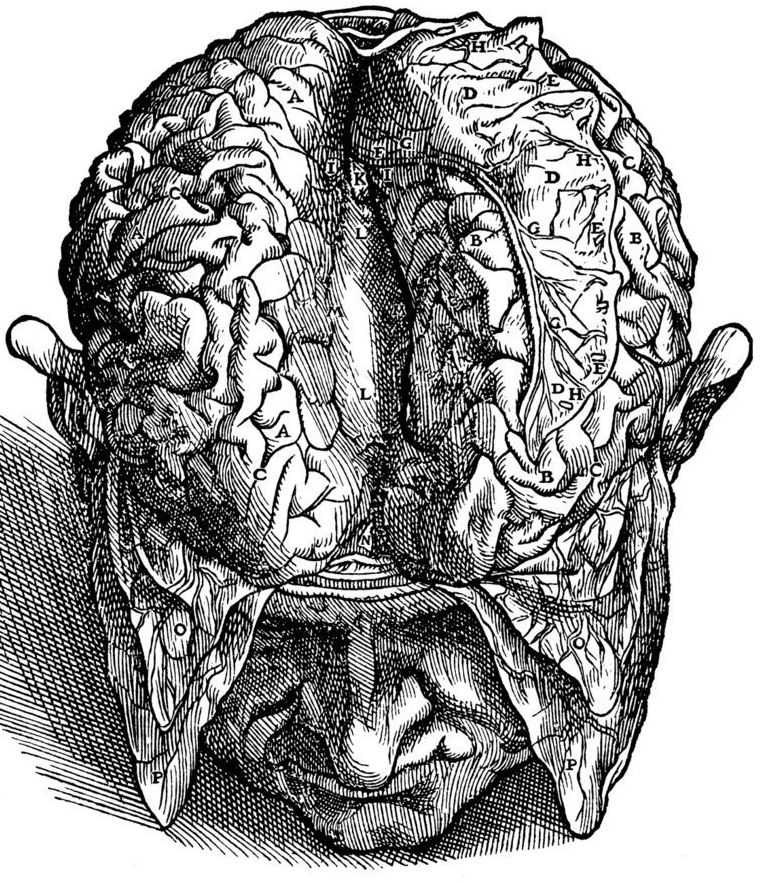
\includegraphics[width=0.7\linewidth]{./figures/nervoussystem/braincase} 

}

\caption{A drawing of the view of the brain by \href{https://en.wikipedia.org/wiki/Andreas_Vesalius}{Andreas Vesalius} (31 December 1514 -- 15 October 1564). Vesalius was a 16th-century Flemish anatomist, physician, and author of one of the most influential books on human anatomy, De humani corporis fabrica (On the Fabric of the Human Body). Vesalius is often referred to as the founder of modern human anatomy. He was born in Brussels, which was then part of the Habsburg Netherlands. He was professor at the University of Padua and later became Imperial physician at the court of Emperor Charles V. Andreas Vesalius is the Latinized form of the Dutch Andries van Wesel. It was a common practice among European scholars in his time to Latinize their names.}\label{fig:braincase}
\end{figure}

The discovery of a staining technique called black reaction by the Italian biologist and pathologist \href{https://en.wikipedia.org/wiki/Camillo_Golgi}{Camillo Golgi} (7 July 1843 -- 21 January 1926) in 1873 was was a major breakthrough in neuroscience. This staining technique is now simply referred to as the Golgi stain. This new method was used with great success by the the Spanish biologist \href{https://en.wikipedia.org/wiki/Santiago_Ramón_y_Cajal}{Santiago Ramón y Cajal} who together with Golgi was given the Nobel Prize in Physiology or Medicine 1906 ``in recognition of their work on the structure of the nervous system''. Cajal's original investigations of the microscopic structure of the brain made him a pioneer of modern neuroscience. Many of his drawings illustrating the delicate arborizations (``tree growing'') of brain cells are included in this text. Cajal discovered the axonal growth cone, and demonstrated experimentally that the relationship between nerve cells was not continuous, but contiguous. This provided definitive evidence for what \href{https://en.wikipedia.org/wiki/Heinrich_Wilhelm_Gottfried_von_Waldeyer-Hartz}{Heinrich Waldeyer} coined the term neuron theory as opposed to the reticular theory (ironically promoted by Golgi whose staining technique was used by Cajal). This is now widely considered the foundation of modern neuroscience.



\begin{figure}

{\centering 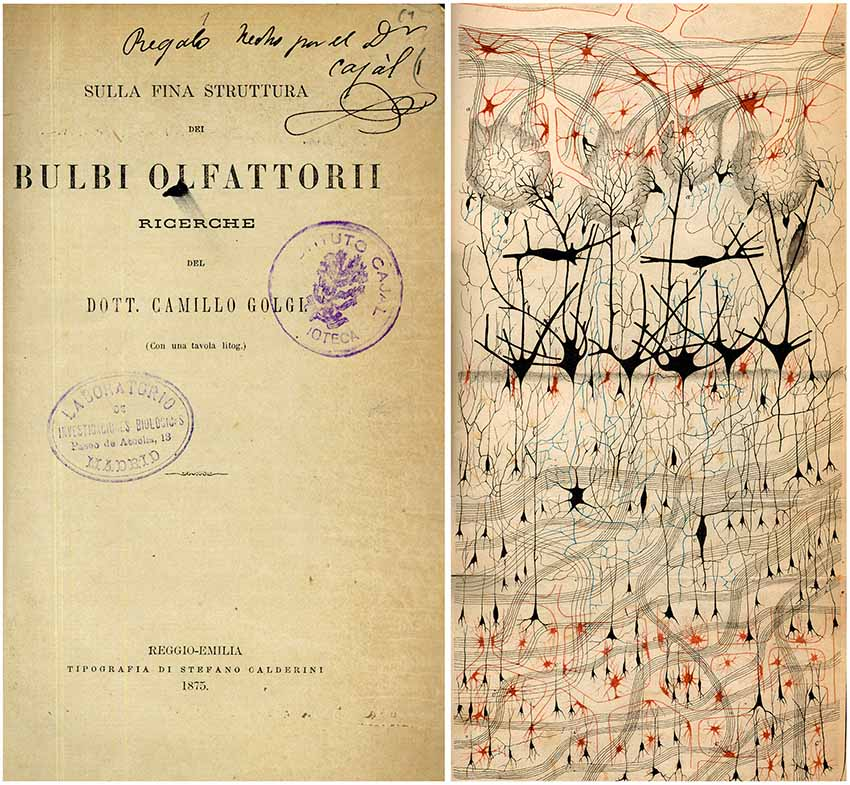
\includegraphics[width=0.7\linewidth]{./figures/nervoussystem/fnana-09-00014-g001} 

}

\caption{\href{https://www.frontiersin.org/articles/10.3389/fnana.2015.00014/full}{The first illustration by Golgi of a Golgi impregnated preparation of the nervous system. ``Semi-schematic drawing of a fragment of a vertical section of the olfactory bulb of a dog''.}.}\label{fig:golgifig}
\end{figure}

The cells in nervous tissue are densely packed and little information on their structures and interconnections can be obtained if all the cells are stained. Furthermore, the thin filamentary extensions of neural cells, including the axon and the dendrites of neurons, are too slender and transparent to be seen with normal staining techniques. Golgi's method stains a limited number of cells at random in their entirety. The mechanism by which this happens is still largely unknown. Dendrites, as well as the cell soma, are clearly stained in brown and black and can be followed in their entire length, which allowed neuroanatomists to track connections between neurons and to make visible the complex networking structure of many parts of the brain and spinal cord.

While the fact that the Golgi method stains only a limited number of neurons allowed the fine structure of the nervous system to be studied in great detail, it limits scientists' ability to delineate the ``connectome'' of the brain. A connectome is a comprehensive map of neural connections in the brain, and may be thought of as its ``wiring diagram''. More broadly, a connectome would include the mapping of all neural connections within an organism's nervous system.
In 2007, a team led by Jeff W. Lichtman and Joshua R. Sanes created a novel technique called ``\href{https://en.wikipedia.org/wiki/Brainbow}{brainbow}''. Brainbow is a process by which individual neurons in the brain can be distinguished from neighboring neurons using fluorescent proteins. By randomly expressing different ratios of red, green, and blue derivatives of green fluorescent protein in individual neurons, it is possible to flag each neuron with a distinctive color. This process has been a major contribution to the field of connectomics, traditionally known as hodology.



\begin{figure}

{\centering 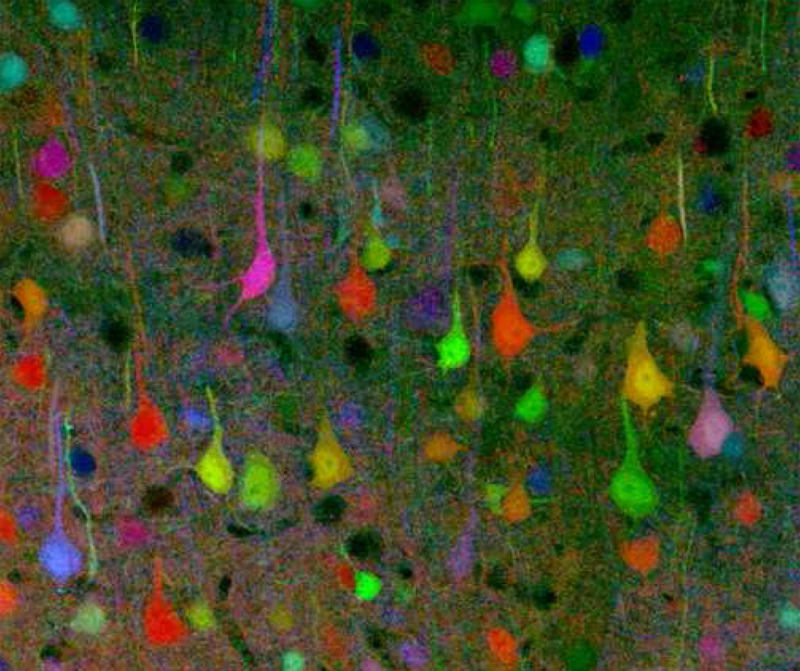
\includegraphics[width=0.7\linewidth]{./figures/nervoussystem/nihms37882f2} 

}

\caption{\href{https://commons.wikimedia.org/wiki/File:Brainbow_(Smith_2007).jpg}{A brainbow of mouse neurons.}}\label{fig:brainbow}
\end{figure}

Neuroscience (or neurobiology) is a multidisciplinary branch of biology that combines physiology, anatomy, molecular biology, developmental biology, cytology, mathematical modeling, and psychology to understand the fundamental and emergent properties of neurons and neural circuits. The understanding of the biological basis of learning, memory, behavior, perception, and consciousness has been described as the ``ultimate challenge'' of the biological sciences. The human brain is often referred to as the most complicated structure in the universe. The scope of neuroscience has broadened over time to include different approaches used to study the nervous system at different scales and the techniques used by neuroscientists have expanded enormously, from molecular and cellular studies of individual neurons to imaging of sensory, motor and cognitive tasks in the brain. Malfunction of the nervous system can occur as a result of genetic defects, physical damage due to trauma or toxicity, infection or simply of ageing. The medical specialty of neurology studies disorders of the nervous system and looks for interventions that can prevent or treat them. Although mental illnesses are believed by many to be neurological disorders affecting the central nervous system, traditionally they are classified separately, and treated by psychiatrists.

Nervous systems are found in most multicellular animals, but vary greatly in complexity. The only multicellular animals that have no nervous system at all are sponges, placozoans, and mesozoans, which have very simple body plans. However, even sponges, unicellular animals, and even protists such as slime molds have cell-to-cell signalling mechanisms that are precursors to those of neurons. The nervous systems of the radially symmetric organisms ctenophores (comb jellies) and cnidarians (which include anemones, hydras, corals and jellyfish) consist of a diffuse nerve net. All other animal species, with the exception of a few types of worm, have a nervous system containing a brain, a central cord (or two cords running in parallel), and nerves radiating from the brain and central cord. The size of the nervous system ranges from a few hundred cells in the simplest worms, to around 300 billion cells in African elephants.

Nervous tissue first arose in wormlike organisms about 550 to 600 million years ago. In humans and other vertebrates it consists of two main parts, the central nervous system (CNS) and the peripheral nervous system (PNS). The CNS consists of the brain and spinal cord. The PNS consists mainly of nerves, which are enclosed bundles of the long fibers or axons, that connect the CNS to every other part of the body. Nerves that transmit signals from the brain are called motor or efferent nerves, while those nerves that transmit information from the body to the CNS are called sensory or afferent. Spinal nerves serve both functions and are called mixed nerves. The PNS is divided into three separate subsystems, the somatic, autonomic, and enteric nervous systems. Somatic nerves carry sensory information from the periphery to the CNS and signals for voluntary movement from the CNS to the muscles. The autonomic nervous system is further subdivided into the sympathetic and the parasympathetic nervous systems. The sympathetic nervous system is activated in cases of emergencies to mobilize energy, while the parasympathetic nervous system is activated when organisms are in a relaxed state. The enteric nervous system functions to control the gastrointestinal system. Both autonomic and enteric nervous systems function involuntarily. Nerves that exit from the cranium are called cranial nerves while those exiting from the spinal cord are called spinal nerves.

\hypertarget{the-cells-of-the-nervous-system}{%
\section{The Cells Of The Nervous System}\label{the-cells-of-the-nervous-system}}

At the cellular level, the nervous system is defined by the presence of a special type of cell, called the neuron, also known as a nerve cell. Neurons have special structures that allow them to receive and send signals from and to other cells. They send these signals in the form of electrochemical waves traveling along thin fibers called axons, which cause chemicals called neurotransmitters to be released at junctions called synapses. Neurons usually receive signalls at tree-like processes called dendrites. A cell that receives a synaptic signal from another neuron may be excited, inhibited, or otherwise modulated. The connections between neurons can form neural pathways, neural circuits, and larger networks that generate an organism's perception of the world and determine its behavior. Along with neurons, the nervous system contains other specialized cells called glial cells (or simply glia), which provide structural and metabolic support.



\begin{figure}

{\centering 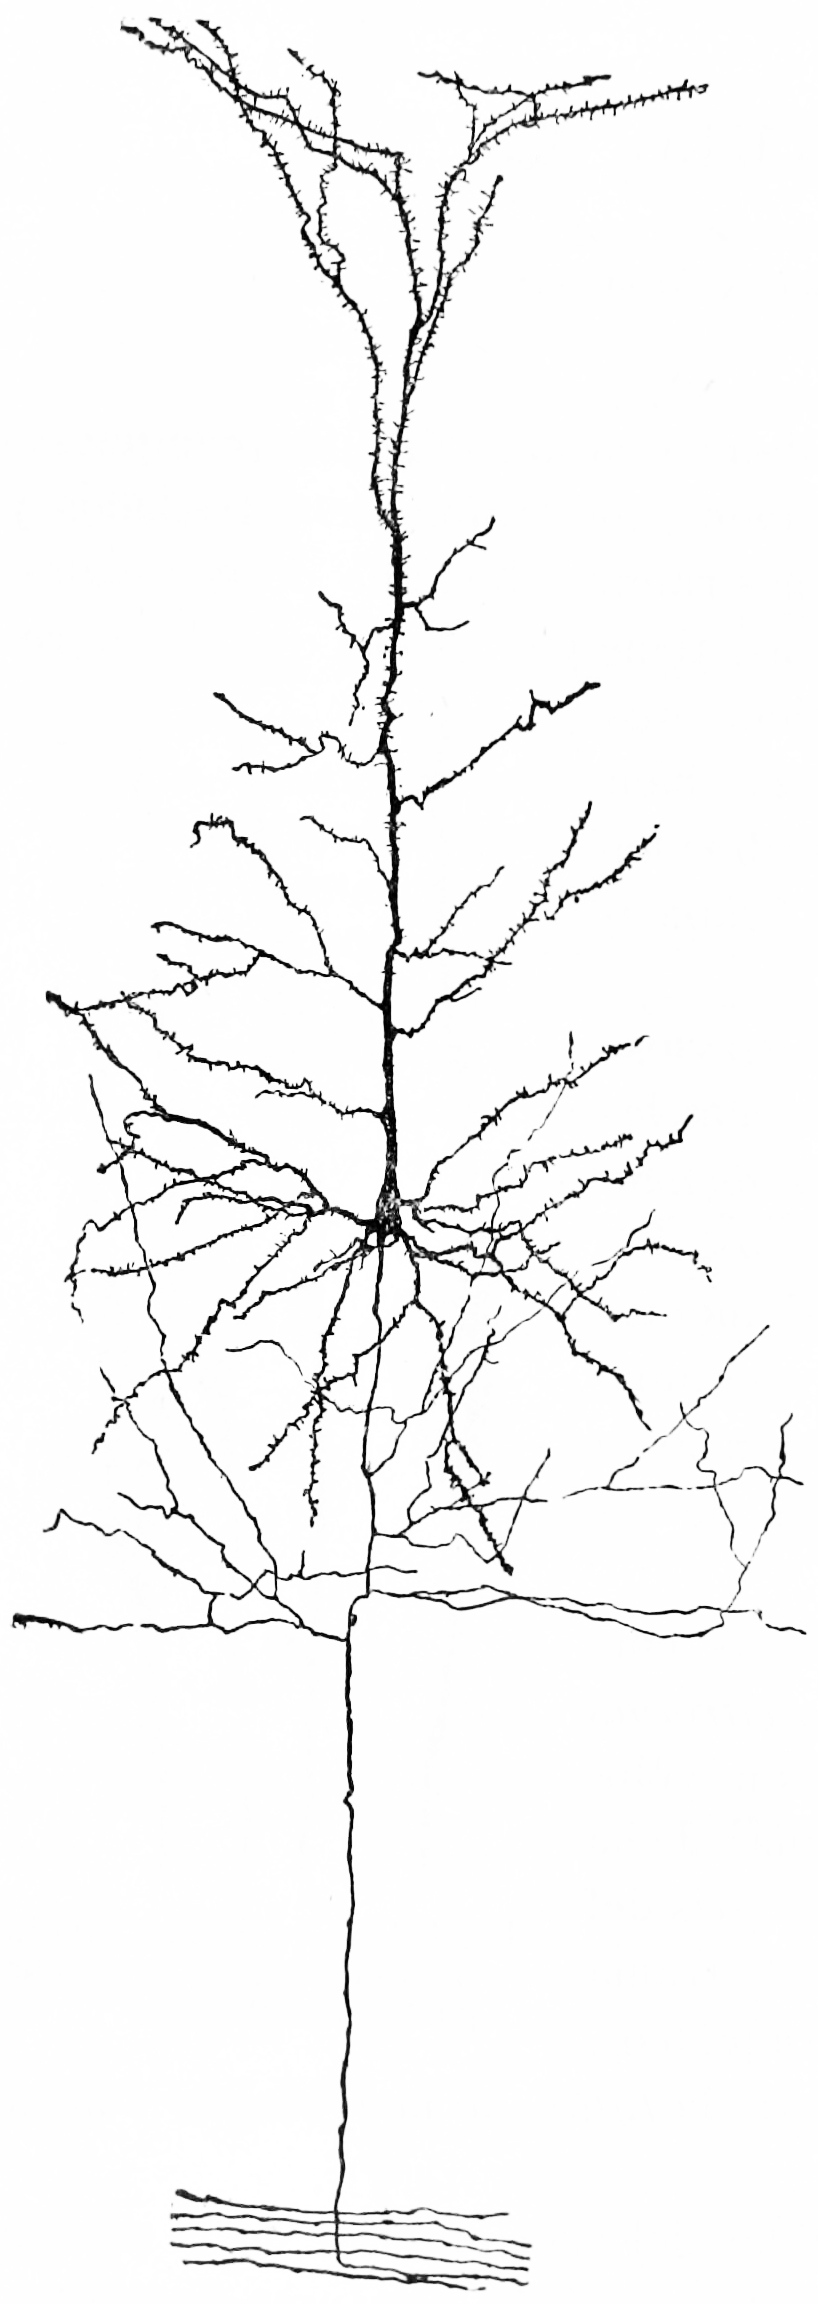
\includegraphics[width=0.7\linewidth]{./figures/cells/RabbitPyramidalCellCajalMetodos} 

}

\caption{A nerve cell from the cerebral cortex of a rabbit. Notice the extensive tree of dendrites at the top, the long axon at the bottom. Because of the pyramid-like shape of the cell body, this type of neuron is referred to as a pyramidal cell.}\label{fig:pyramidalcell}
\end{figure}

Even in the nervous system of a single species such as humans, hundreds of different types of neurons exist, with a wide variety of morphologies and functions. These include sensory neurons that convert physical stimuli such as light and sound into neural signals, and motor neurons that activate muscles or glands; however in many species the great majority of neurons participate in the formation of centralized structures (the brain and ganglia) and they receive all of their input from other neurons and send their output to other neurons.

Glial cells (named from the Greek for ``glue'') are non-neuronal cells that provide support and nutrition, maintain homeostasis, form myelin, and participate in signal transmission in the nervous system. In the human brain, it is estimated that the total number of glia roughly equals the number of neurons, although the proportions vary in different brain areas. Among the most important functions of glial cells are to support neurons and hold them in place; to supply nutrients to neurons; to insulate neurons electrically; to destroy pathogens and remove dead neurons; and to provide guidance cues directing the axons of neurons to their targets. A very important type of glial cell (oligodendrocytes in the central nervous system, and Schwann cells in the peripheral nervous system) generates layers of a fatty substance called myelin that wraps around axons and provides electrical insulation which allows them to transmit action potentials much more rapidly and efficiently. Microglia serve as important resident immune cells within the central nervous system.

\hypertarget{comparative-anatomy-and-evolution-of-nervous-systems}{%
\section{Comparative Anatomy And Evolution Of Nervous Systems}\label{comparative-anatomy-and-evolution-of-nervous-systems}}

Porifera (sponges) have no cells connected to each other by synaptic junctions, that is, no neurons, and therefore no nervous system. They do, however, have homologs of many genes that play key roles in synaptic function. Recent studies have shown that sponge cells express a group of proteins that cluster together to form a structure resembling a postsynaptic density (the signal-receiving part of a synapse). However, the function of this structure is currently unclear. Although sponge cells do not show synaptic transmission, they do communicate with each other via calcium waves and other impulses, which mediate some simple actions such as whole-body contraction.

Radiata such as the cnidaria (jellyfish) and ctenophora (comb jellies) have diffuse nerve nets rather than a central nervous system. In most jellyfish the nerve net is spread more or less evenly across the body; in comb jellies it is concentrated near the mouth. The nerve nets consist of sensory neurons, which pick up chemical, tactile, and visual signals; motor neurons, which can activate contractions of the body wall; and intermediate neurons, which detect patterns of activity in the sensory neurons and, in response, send signals to groups of motor neurons. In some cases groups of intermediate neurons are clustered into discrete ganglia.

The development of the nervous system in radiata is relatively unstructured. Unlike bilaterians, radiata only have two primordial cell layers, endoderm and ectoderm. Neurons are generated from a special set of ectodermal precursor cells, which also serve as precursors for every other ectodermal cell type.

The vast majority of existing animals are bilaterians, meaning animals with left and right sides that are approximate mirror images of each other. All bilateria are thought to have descended from a common wormlike ancestor that appeared in the Ediacaran period, 550--600 million years ago. The fundamental bilaterian body form is a tube with a hollow gut cavity running from mouth to anus, and a nerve cord with an enlargement (a ``ganglion'') for each body segment, with an especially large ganglion at the front, called the ``brain''.



\begin{figure}

{\centering \includegraphics[width=0.7\linewidth]{./figures/nervoussystem/invertebrate_nervoussystems} 

}

\caption{Comparison of nervous systems of invertebrates. Top left: A diffuse nerve net in \emph{Actinia} (a genus of sea anemones in the family \emph{Actiniidae} in the phylum \emph{Cnidaria}); top right: The nervous system of \emph{Anadonta anatina}, a freshwater mussel in the family \emph{Unionidae} in the phylum \emph{Mollusca}. c, foot; k, pedal ganglion; i, cerebro-pedal connective; g, cerebral ganglion; h, cerebral connective; a, anterior adductor muscle; r, q, anterior pallial nerves; d, liver; s, visceral nerve; l, cerebro-visceral connective; e, gill; f, edge of mantle; n, branchial nerves; m, visceral ganglion; o, posterior pallial nerves; b, posterior adductor muscle; p, lateral pallial nerves; bottom left: the nervous system of \emph{Alitta virens}, a polychaete worm in the phylum \emph{Annelida}. J, jaws; b, antennal nerves; c, palpal nerves; f, ganglia for the dorsal peristomial cirri; n\textsuperscript{1} , ganglion; n, nerves for the dissepimenta; m, parapodial nerves; i, parapodial branch; h, ventral chain of ganglia; C, cerebral ganglion; o, nerve passing through dissepiment to preceding segment; k, parapodial ganglion. Bottom right: the nervous system of an insect (\emph{Arthropoda}). From \href{https://www.biodiversitylibrary.org/ia/morphologyofinve00petr\#page/7/mode/1up}{Morphology of invertebrate types, by Alexander Petrunkevitch. New York, Macmillan company, 1916.}}\label{fig:invertebratenervoussystem}
\end{figure}

Even mammals, including humans, show the segmented bilaterian body plan at the level of the nervous system. The spinal cord contains a series of segmental ganglia, each giving rise to motor and sensory nerves that innervate a portion of the body surface and underlying musculature. On the limbs, the layout of the innervation pattern is complex, but on the trunk it gives rise to a series of narrow bands. The top three segments belong to the brain, giving rise to the forebrain, midbrain, and hindbrain.

Bilaterians can be divided, based on events that occur very early in embryonic development, into two groups (superphyla) called protostomes and deuterostomes. Deuterostomes include vertebrates as well as echinoderms, hemichordates (mainly acorn worms), and Xenoturbellidans. Protostomes, the more diverse group, include arthropods, molluscs, and numerous types of worms. There is a basic difference between the two groups in the placement of the nervous system within the body: protostomes possess a nerve cord on the ventral (usually bottom) side of the body, whereas in deuterostomes the nerve cord is on the dorsal (usually top) side. In fact, numerous aspects of the body are inverted between the two groups, including the expression patterns of several genes that show dorsal-to-ventral gradients. Most anatomists now consider that the bodies of protostomes and deuterostomes are ``flipped over'' with respect to each other, a hypothesis that was first proposed by Geoffroy Saint-Hilaire for insects in comparison to vertebrates. Thus insects, for example, have nerve cords that run along the ventral midline of the body, while all vertebrates have spinal cords that run along the dorsal midline.

There are a few types of existing bilaterians that lack a recognizable brain, including echinoderms and tunicates. It has not been definitively established whether the existence of these brainless species indicates that the earliest bilaterians lacked a brain, or whether their ancestors evolved in a way that led to the disappearance of a previously existing brain structure.

The diversity of invertebrate body plans is matched by an equal diversity in brain structures. Two groups of invertebrates have notably complex brains: arthropods (insects, crustaceans, arachnids, and others), and cephalopods (octopuses, squids, and similar molluscs). The brains of arthropods and cephalopods arise from twin parallel nerve cords that extend through the body of the animal. Arthropods have a central brain, the supraesophageal ganglion, with three divisions and large optical lobes behind each eye for visual processing. Cephalopods such as the octopus and squid have the largest brains of any invertebrates.

There are several invertebrate species whose brains have been studied intensively because they have properties that make them convenient for experimental work:

\begin{itemize}
\tightlist
\item
  Fruit flies (\emph{Drosophila melanogaster}), because of the large array of techniques available for studying their genetics, have been a natural subject for studying the role of genes in brain development. In spite of the large evolutionary distance between insects and mammals, many aspects of \emph{Drosophila} neurogenetics have been shown to be relevant to humans. The first biological clock genes, for example, were identified by examining \emph{Drosophila} mutants that showed disrupted daily activity cycles. A search in the genomes of vertebrates revealed a set of analogous genes, which were found to play similar roles in the mouse biological clock---and therefore almost certainly in the human biological clock as well. Studies done on Drosophila, also show that most neuropil regions of the brain are continuously reorganized throughout life in response to specific living conditions.
\item
  The nematode worm \emph{Caenorhabditis elegans}, like Drosophila, has been studied largely because of its importance in genetics. In the early 1970s, \href{https://en.wikipedia.org/wiki/Sydney_Brenner}{Sydney Brenner} chose it as a model organism for studying the way that genes control development. One of the advantages of working with this worm is that the body plan is very stereotyped: the nervous system of the hermaphrodite contains exactly 302 neurons, always in the same places, making identical synaptic connections in every worm. Brenner's team sliced worms into thousands of ultrathin sections and photographed each one under an electron microscope, then visually matched fibers from section to section, to map out every neuron and synapse in the entire body. The complete neuronal wiring diagram of \emph{C. elegans} -- its connectome was achieved. Nothing approaching this level of detail is available for any other organism, and the information gained has enabled a multitude of studies that would otherwise have not been possible.
\item
  The sea slug \emph{Aplysia californica} was chosen by Nobel Prize-winning neurophysiologist \href{https://en.wikipedia.org/wiki/Eric_Kandel}{Eric Kandel} as a model for studying the cellular basis of learning and memory, because of the simplicity and accessibility of its nervous system, and it has been examined in hundreds of experiments.
\end{itemize}

Worms are the simplest bilaterian animals, and reveal the basic structure of the bilaterian nervous system in the most straightforward way. As an example, earthworms have dual nerve cords running along the length of the body and merging at the tail and the mouth. These nerve cords are connected by transverse nerves like the rungs of a ladder. These transverse nerves help coordinate the two sides of the animal. Two ganglia at the head (the ``nerve ring'') end function similar to a simple brain. Photoreceptors on the animal's eyespots provide sensory information on light and dark.

Arthropods, such as insects and crustaceans, have a nervous system made up of a series of ganglia, connected by a ventral nerve cord made up of two parallel connectives running along the length of the belly. Typically, each body segment has one ganglion on each side, though some ganglia are fused to form the brain and other large ganglia. The head segment contains the brain, also known as the supraesophageal ganglion. In the insect nervous system, the brain is anatomically divided into the protocerebrum, deutocerebrum, and tritocerebrum. Immediately behind the brain is the subesophageal ganglion, which is composed of three pairs of fused ganglia. It controls the mouthparts, the salivary glands and certain muscles. Many arthropods have well-developed sensory organs, including compound eyes for vision and antennae for olfaction and pheromone sensation. The sensory information from these organs is processed by the brain.

In insects, many neurons have cell bodies that are positioned at the edge of the brain and are electrically passive---the cell bodies serve only to provide metabolic support and do not participate in signalling. A protoplasmic fiber runs from the cell body and branches profusely, with some parts transmitting signals and other parts receiving signals. Thus, most parts of the insect brain have passive cell bodies arranged around the periphery, while the neural signal processing takes place in a tangle of protoplasmic fibers called neuropil, in the interior.

Brains are most simply compared in terms of their size. The relationship between brain size, body size and other variables has been studied across a wide range of vertebrate species. As a rule, brain size increases with body size, but not in a simple linear proportion. In general, smaller animals tend to have larger brains, measured as a fraction of body size. For mammals, the relationship between brain volume and body mass essentially follows a power law with an exponent of about 0.75. This formula describes the central tendency, but every family of mammals departs from it to some degree, in a way that reflects in part the complexity of their behavior. For example, primates have brains 5 to 10 times larger than the formula predicts. Predators tend to have larger brains than their prey, relative to body size.

All vertebrate brains share a common underlying form, which appears most clearly during early stages of embryonic development. In its earliest form, the brain appears as three swellings at the front end of the neural tube; these swellings eventually become the forebrain, midbrain, and hindbrain (the prosencephalon, mesencephalon, and rhombencephalon, respectively). At the earliest stages of brain development, the three areas are roughly equal in size. In many classes of vertebrates, such as fish and amphibians, the three parts remain similar in size in the adult, but in mammals the forebrain becomes much larger than the other parts, and the midbrain becomes very small.



\begin{figure}

{\centering 
\includegraphics[width=0.7\linewidth]{./figures/nervoussystem/cns_comparison} 

}

\caption{Dorsal views of the central nervous systems of the teleosts (from left to right) \emph{Trigla hirundo} (a) and \emph{Mola mola}, the urodele \emph{Ambystoma tigrinum}, the anuran \emph{Xenopus laevis}, the tortoise \emph{Testudo hermanni}, the tegu lizard \emph{Tupinambis teguixin}, the pigeon, the cat and human. In a, c, d, e, f, g and j the full length of the spinalcord, including the filum terminale (where present) is shown; in \emph{Mola mola} and the cat most of the filum terminale is cut. Vertical black bars correspond to 1 cm in length. Modified from \href{https://doi.org/10.1007/978-3-642-18262-4_24}{Nieuwenhuys, R., ten Donkelaar, H. J., \& Nicholson, C. (1998). The Meaning of It All. The Central Nervous System of Vertebrates, 2135--2195}}\label{fig:vertebratecns}
\end{figure}

The brains of vertebrates are made of very soft tissue. Living brain tissue is pinkish on the outside and mostly white on the inside, with subtle variations in color. Vertebrate brains are surrounded by a system of connective tissue membranes called meninges that separate the skull from the brain. Blood vessels enter the central nervous system through holes in the meningeal layers. The cells in the blood vessel walls are joined tightly to one another, forming the blood--brain barrier, which blocks the passage of many toxins and pathogens (though at the same time blocking antibodies and some drugs, thereby presenting special challenges in treatment of diseases of the brain).

Neuroanatomists usually divide the vertebrate brain into six main regions: the telencephalon (cerebral hemispheres), diencephalon (thalamus and hypothalamus), mesencephalon (midbrain), cerebellum, pons, and medulla oblongata. Each of these areas has a complex internal structure. Some parts, such as the cerebral cortex and the cerebellar cortex, consist of layers that are folded or convoluted to fit within the available space. Other parts, such as the thalamus and hypothalamus, consist of clusters of many small nuclei. Thousands of distinguishable areas can be identified within the vertebrate brain based on fine distinctions of neural structure, chemistry, and connectivity.

There is an anatomical convention that a cluster of neurons in the brain or spinal cord is called a nucleus, whereas a cluster of neurons in the periphery is called a ganglion. There are, however, a few exceptions to this rule, notably including the part of the forebrain called the basal ganglia.

Although the same basic components are present in all vertebrate brains, some branches of vertebrate evolution have led to substantial distortions of brain geometry, especially in the forebrain area. The brain of a shark shows the basic components in a straightforward way, but in teleost fishes (the great majority of existing fish species), the forebrain has become ``everted'', like a sock turned inside out. In birds, there are also major changes in forebrain structure. These distortions can make it difficult to match brain components from one species with those of another species.

Here is a list of some of the most important vertebrate brain components, along with a brief description of their functions as currently understood:

\begin{itemize}
\tightlist
\item
  The medulla, along with the spinal cord, contains many small nuclei involved in a wide variety of sensory and involuntary motor functions such as vomiting, heart rate and digestive processes.
\item
  The pons lies in the brainstem directly above the medulla. Among other things, it contains nuclei that control often voluntary but simple acts such as sleep, respiration, swallowing, bladder function, equilibrium, eye movement, facial expressions, and posture.
\item
  The hypothalamus is a small region at the base of the forebrain, whose complexity and importance belies its size. It is composed of numerous small nuclei, each with distinct connections and neurochemistry. The hypothalamus is engaged in additional involuntary or partially voluntary acts such as sleep and wake cycles, eating and drinking, and the release of some hormones.
\item
  The thalamus is a collection of nuclei with diverse functions: some are involved in relaying information to and from the cerebral hemispheres, while others are involved in motivation. The subthalamic area (zona incerta) seems to contain action-generating systems for several types of ``consummatory'' behaviors such as eating, drinking, defecation, and copulation.
\item
  The cerebellum modulates the outputs of other brain systems, whether motor related or thought related, to make them certain and precise. Removal of the cerebellum does not prevent an animal from doing anything in particular, but it makes actions hesitant and clumsy. This precision is not built-in, but learned by trial and error. The muscle coordination learned while riding a bicycle is an example of a type of neural plasticity that may take place largely within the cerebellum. 10\% of the brain's total volume consists of the cerebellum and 50\% of all neurons are held within its structure.
\item
  The optic tectum allows actions to be directed toward points in space, most commonly in response to visual input. In mammals it is usually referred to as the superior colliculus, and its best-studied function is to direct eye movements. It also directs reaching movements and other object-directed actions. It receives strong visual inputs, but also inputs from other senses that are useful in directing actions, such as auditory input in owls and input from the thermosensitive pit organs in snakes. In some primitive fishes, such as lampreys, this region is the largest part of the brain. The superior colliculus is part of the midbrain.
\item
  The pallium is a layer of gray matter that lies on the surface of the forebrain and is the most complex and most recent evolutionary development of the brain as an organ. In reptiles and mammals, it is called the cerebral cortex. Multiple functions involve the pallium, including smell and spatial memory. In mammals, where it becomes so large as to dominate the brain, it takes over functions from many other brain areas. In many mammals, the cerebral cortex consists of folded bulges called gyri that create deep furrows or fissures called sulci. The folds increase the surface area of the cortex and therefore increase the amount of gray matter and the amount of information that can be stored and processed.
\item
  The hippocampus, strictly speaking, is found only in mammals. However, the area it derives from, the medial pallium, has counterparts in all vertebrates. There is evidence that this part of the brain is involved in complex events such as spatial memory and navigation in fishes, birds, reptiles, and mammals.
\item
  The basal ganglia are a group of interconnected structures in the forebrain. The primary function of the basal ganglia appears to be action selection: they send inhibitory signals to all parts of the brain that can generate motor behaviors, and in the right circumstances can release the inhibition, so that the action-generating systems are able to execute their actions. Reward and punishment exert their most important neural effects by altering connections within the basal ganglia.
\item
  The olfactory bulb is a special structure that processes olfactory sensory signals and sends its output to the olfactory part of the pallium. It is a major brain component in many vertebrates, but is greatly reduced in humans and other primates (whose senses are dominated by information acquired by sight rather than smell).
\end{itemize}

The most obvious difference between the brains of mammals and other vertebrates is in terms of size. On average, a mammal has a brain roughly twice as large as that of a bird of the same body size, and ten times as large as that of a reptile of the same body size.

Size, however, is not the only difference: there are also substantial differences in shape. The hindbrain and midbrain of mammals are generally similar to those of other vertebrates, but dramatic differences appear in the forebrain, which is greatly enlarged and also altered in structure. The cerebral cortex is the part of the brain that most strongly distinguishes mammals. In non-mammalian vertebrates, the surface of the cerebrum is lined with a comparatively simple three-layered structure called the pallium. In mammals, the pallium evolves into a complex six-layered structure called neocortex or isocortex. Several areas at the edge of the neocortex, including the hippocampus and amygdala, are also much more extensively developed in mammals than in other vertebrates.

The elaboration of the cerebral cortex carries with it changes to other brain areas. The superior colliculus, which plays a major role in visual control of behavior in most vertebrates, shrinks to a small size in mammals, and many of its functions are taken over by visual areas of the cerebral cortex. The cerebellum of mammals contains a large portion (the neocerebellum) dedicated to supporting the cerebral cortex, which has no counterpart in other vertebrates.

The brains of humans and other primates contain the same structures as the brains of other mammals, but are generally larger in proportion to body size. The encephalization quotient (EQ) is used to compare brain sizes across species. It takes into account the nonlinearity of the brain-to-body relationship. Humans have an average EQ in the 7-to-8 range, while most other primates have an EQ in the 2-to-3 range. Dolphins have values higher than those of primates other than humans, but nearly all other mammals have EQ values that are substantially lower.



\begin{figure}

{\centering 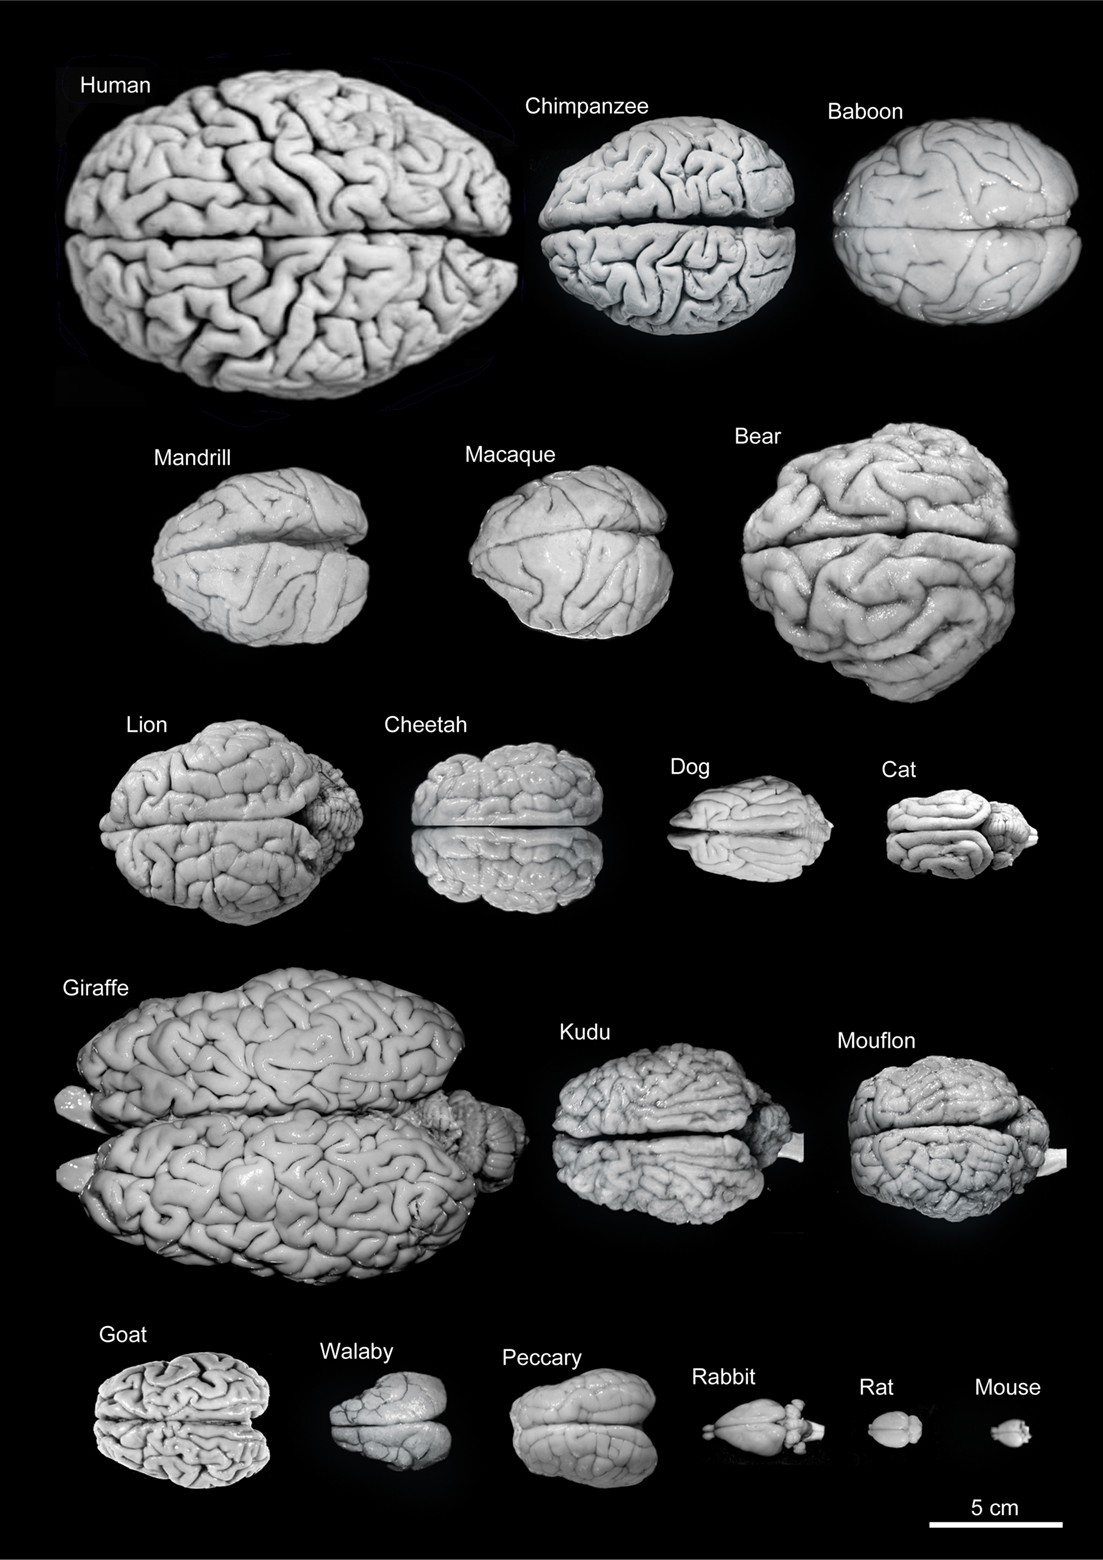
\includegraphics[width=0.7\linewidth]{./figures/nervoussystem/fnana-05-00029-g007} 

}

\caption{Variability of brain size and external topography. Photographs and weights of the brains of different species. Primates: human (Homo sapiens, 1.176 kg), chimpanzee (Pan troglodytes, 273 g), baboon (Papio cynocephalus, 151 g), mandrill (Mandrillus sphinx, 123 g), macaque (Macaca tonkeana, 110 g). Carnivores: bear (Ursus arctos, 289 g), lion (Panthera leo, 165 g), cheetah (Acinonyx jubatus, 119 g), dog (Canis familiaris, 95 g), cat (Felis catus, 32 g). Artiodactyls: giraffe (Giraffa camelopardalis, 700 g), kudu (Tragelaphus strepsiceros, 166 g), mouflon (Ovis musimon, 118 g), ibex (Capra pyrenaica, 115 g); peccary (Tayassu pecari, 41 g). Marsupials: wallaby (Protemnodon rufogrisea, 28 g). Lagomorphs: rabbit (Oryctolagus cuniculus, 5.2 g). Rodents: rat (Rattus rattus, 2.6 g), mouse (Mus musculus, 0.5 g). The chimpanzee brain was kindly supplied by Dr.~Dean Falk. The rest of non-human brains were from material used in Ballesteros-Yánez et al., 2005). Scale bar: 5 cm. From \href{https://www.frontiersin.org/article/10.3389/fnana.2011.00029}{DeFelipe J (2011) The evolution of the brain, the human nature of cortical circuits, and intellectual creativity. Front. Neuroanat. 5:29}}\label{fig:mammaliancns}
\end{figure}

Most of the enlargement of the primate brain comes from a massive expansion of the cerebral cortex, especially the prefrontal cortex and the parts of the cortex involved in vision. The visual processing network of primates includes at least 30 distinguishable brain areas, with a complex web of interconnections. It has been estimated that visual processing areas occupy more than half of the total surface of the primate neocortex. The prefrontal cortex carries out functions that include planning, working memory, motivation, attention, and executive control. It takes up a much larger proportion of the brain for primates than for other species, and an especially large fraction of the human brain.

The peripheral nervous system (PNS) is a collective term for the nervous system structures that do not lie within the CNS. The large majority of the axon bundles called nerves are considered to belong to the PNS, even when the cell bodies of the neurons to which they belong reside within the brain or spinal cord. The PNS is divided into somatic and visceral parts. The somatic part consists of the nerves that innervate the skin, joints, and muscles. The cell bodies of somatic sensory neurons lie in dorsal root ganglia of the spinal cord. The visceral part, also known as the autonomic nervous system, contains neurons that innervate the internal organs, blood vessels, and glands. The autonomic nervous system itself consists of two parts: the sympathetic nervous system and the parasympathetic nervous system. Some authors also include sensory neurons whose cell bodies lie in the periphery (for senses such as hearing) as part of the PNS; others, however, omit them.

The vertebrate nervous system can also be divided into areas called gray matter and white matter. Gray matter (which is only gray in preserved tissue, and is better described as pink or light brown in living tissue) contains a high proportion of cell bodies of neurons. White matter is composed mainly of myelinated axons, and takes its color from the myelin. White matter includes all of the nerves, and much of the interior of the brain and spinal cord. Gray matter is found in clusters of neurons in the brain and spinal cord, and in cortical layers that line their surfaces.

\hypertarget{the-human-brain}{%
\section{The Human Brain}\label{the-human-brain}}

The adult human brain weighs on average about 1.2--1.4 kg (2.6--3.1 lb) which is about 2\% of the total body weight, with a volume of around 1260 cm\textsuperscript{3} in men and 1130 cm\textsuperscript{3} in women. There is substantial individual variation, with the standard reference range for men being 1,180--1,620 g (2.60--3.57 lb) and for women 1,030--1,400 g (2.27--3.09 lb).

The human brain is divided into nearly symmetrical left and right hemispheres by a deep groove, the longitudinal fissure. Each hemisphere is conventionally divided into four main lobes; the frontal lobe, parietal lobe, temporal lobe, and occipital lobe, named according to the skull bones that overlie them. The surface of the brain is folded into ridges (gyri) and grooves (sulci), many of which are named, usually according to their position, such as the frontal gyrus of the frontal lobe or the central sulcus separating the central regions of the hemispheres. There are many small variations in the secondary and tertiary folds.



\begin{figure}

{\centering 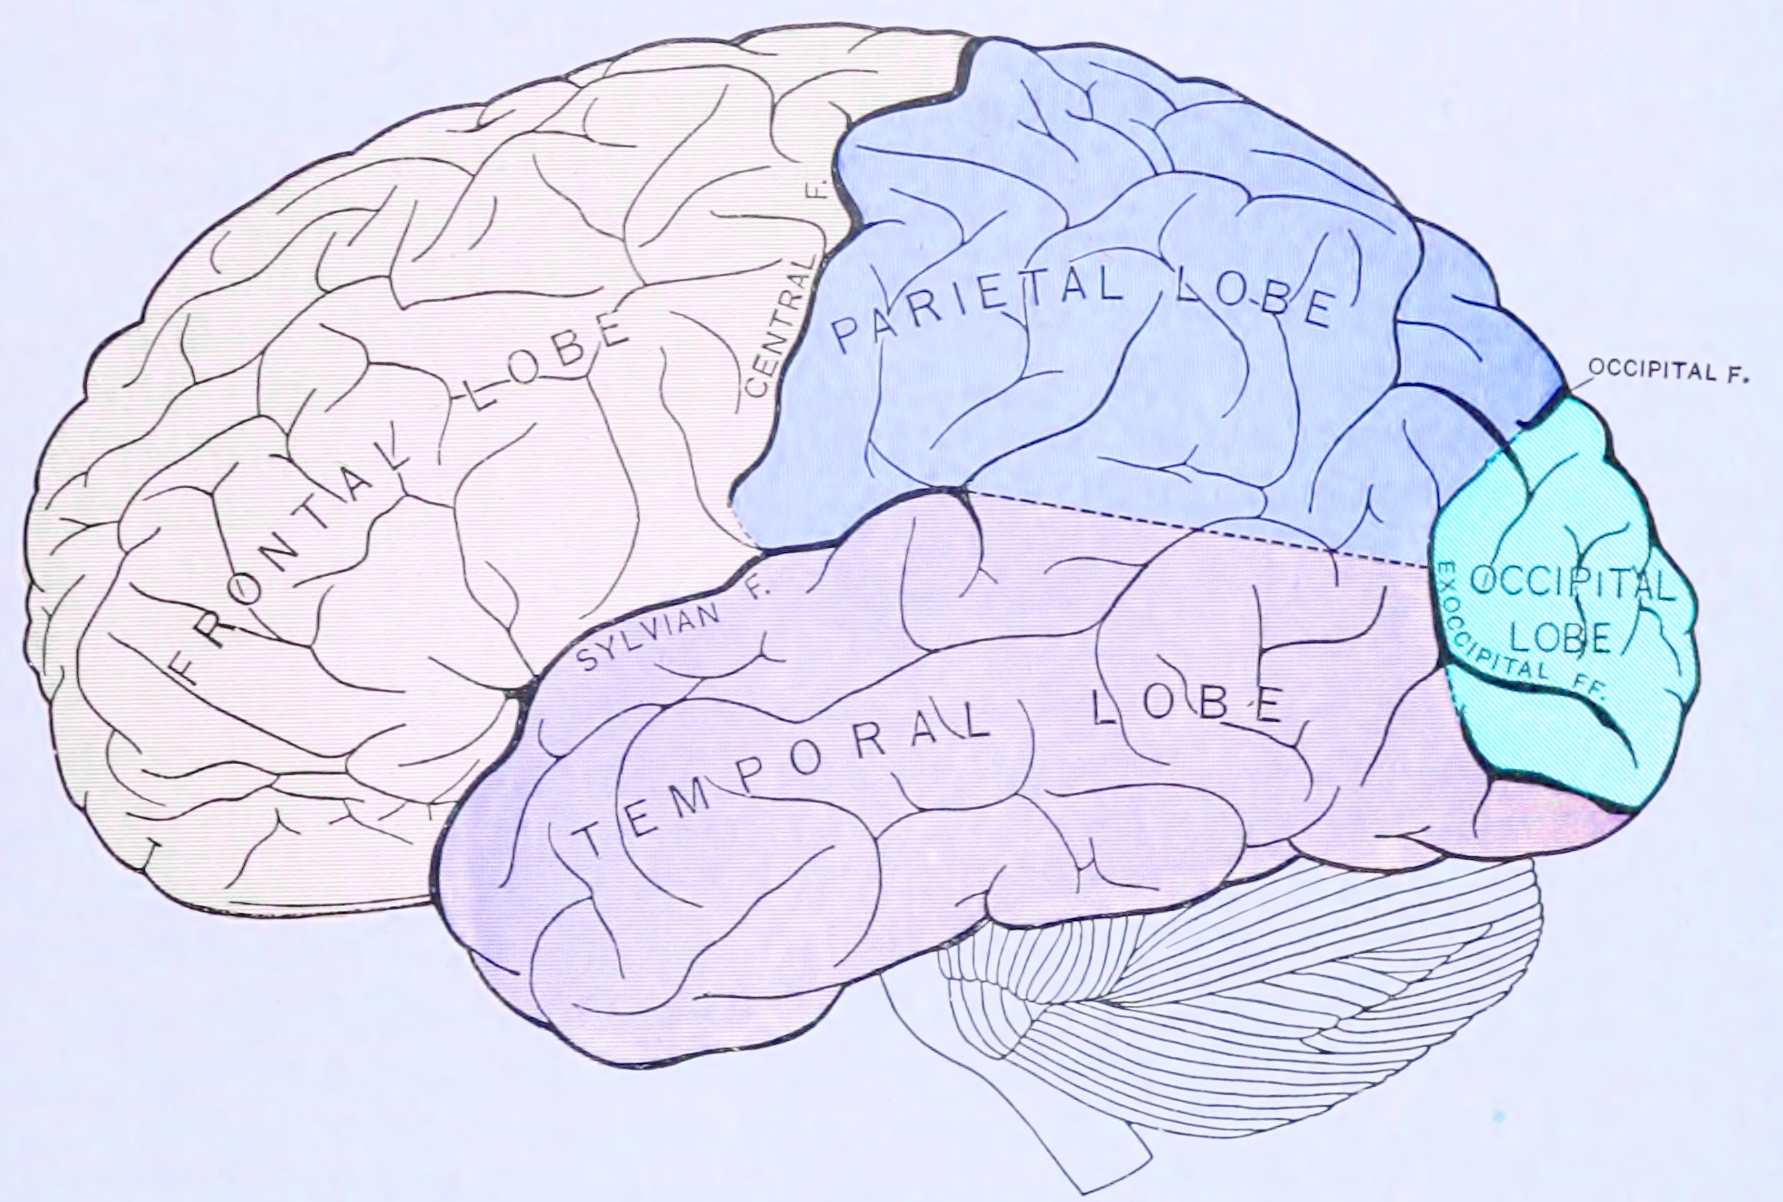
\includegraphics[width=0.7\linewidth]{./figures/nervoussystem/GrayAnat1918p821} 

}

\caption{Principal lobes and fissures of the cerebrum viewed laterally. From \href{https://archive.org/details/anatomyofhumanbo1918gray/page/n6/mode/2up}{Gray Henry, Anatomy of the Human Body. 20\textsuperscript{th} Edition, Lea \& Febiger, Philadelphia \& New York, 1918}}\label{fig:principallobes}
\end{figure}



\begin{figure}

{\centering 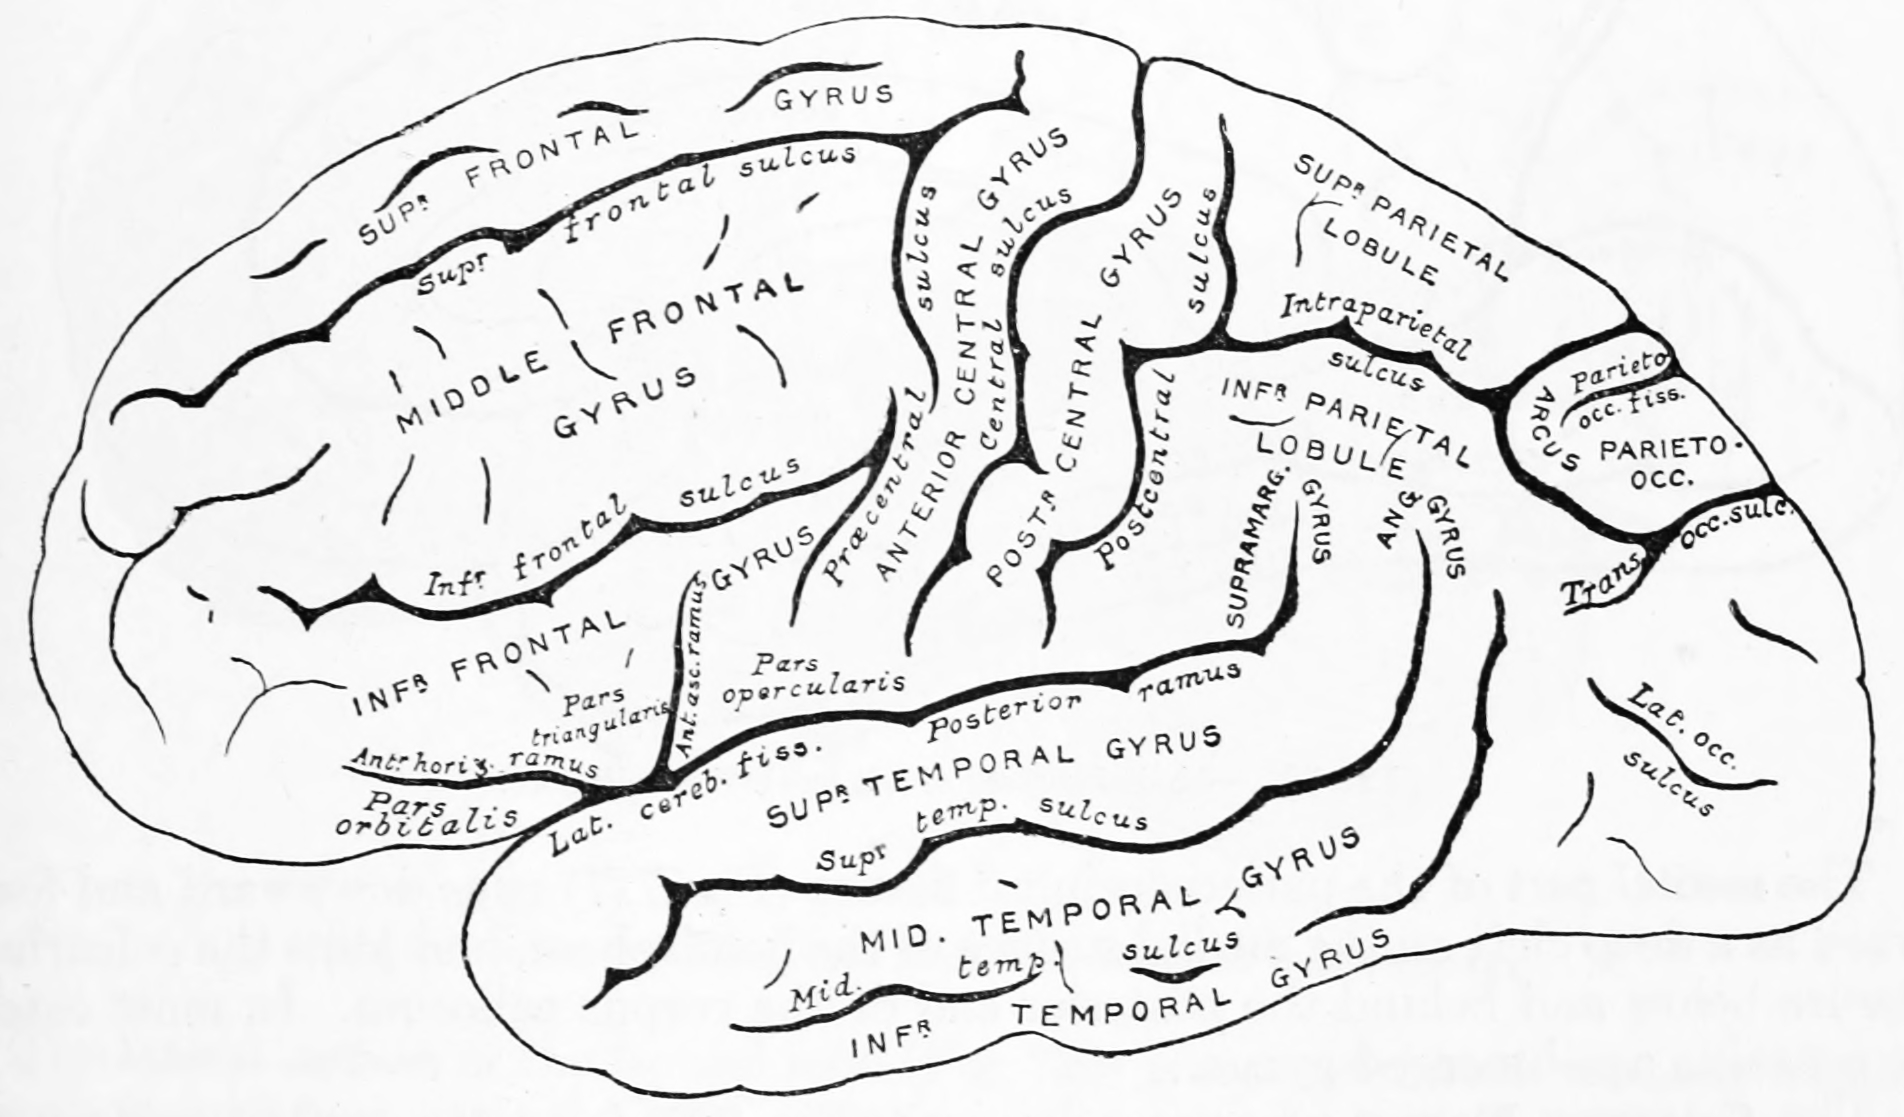
\includegraphics[width=0.7\linewidth]{./figures/nervoussystem/GrayAnat1918p819} 

}

\caption{Diagram showing a lateral view of the ridges (gyri) and grooves (sulci) of the left hemisphere of the brain. From \href{https://archive.org/details/anatomyofhumanbo1918gray/page/n6/mode/2up}{Gray Henry, Anatomy of the Human Body. 20\textsuperscript{th} Edition, Lea \& Febiger, Philadelphia \& New York, 1918}}\label{fig:gyrilateral}
\end{figure}



\begin{figure}

{\centering 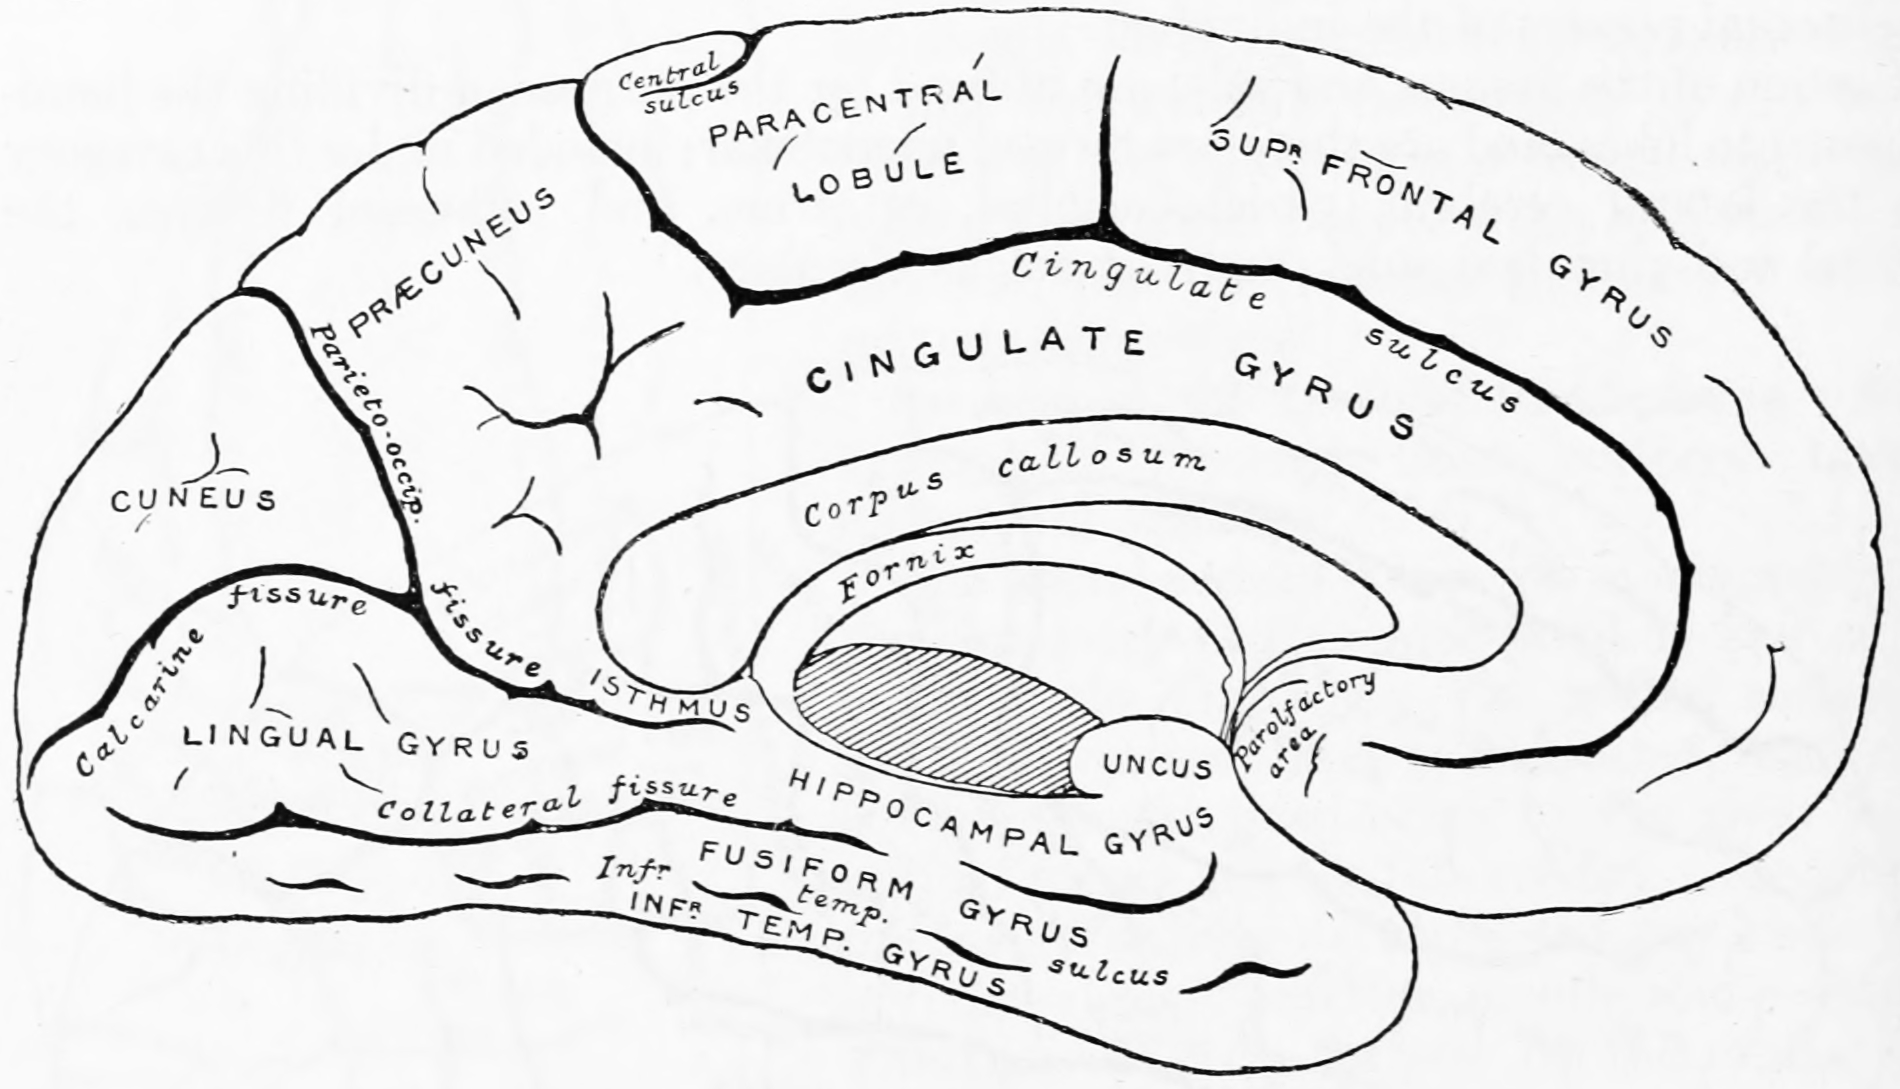
\includegraphics[width=0.7\linewidth]{./figures/nervoussystem/GrayAnat1918p820} 

}

\caption{Diagram showing a medial view of the ridges (gyri) and grooves (sulci) of the left hemisphere of the brain. From \href{https://archive.org/details/anatomyofhumanbo1918gray/page/n6/mode/2up}{Gray Henry, Anatomy of the Human Body. 20\textsuperscript{th} Edition, Lea \& Febiger, Philadelphia \& New York, 1918}}\label{fig:gyrimedial}
\end{figure}



\begin{figure}

{\centering 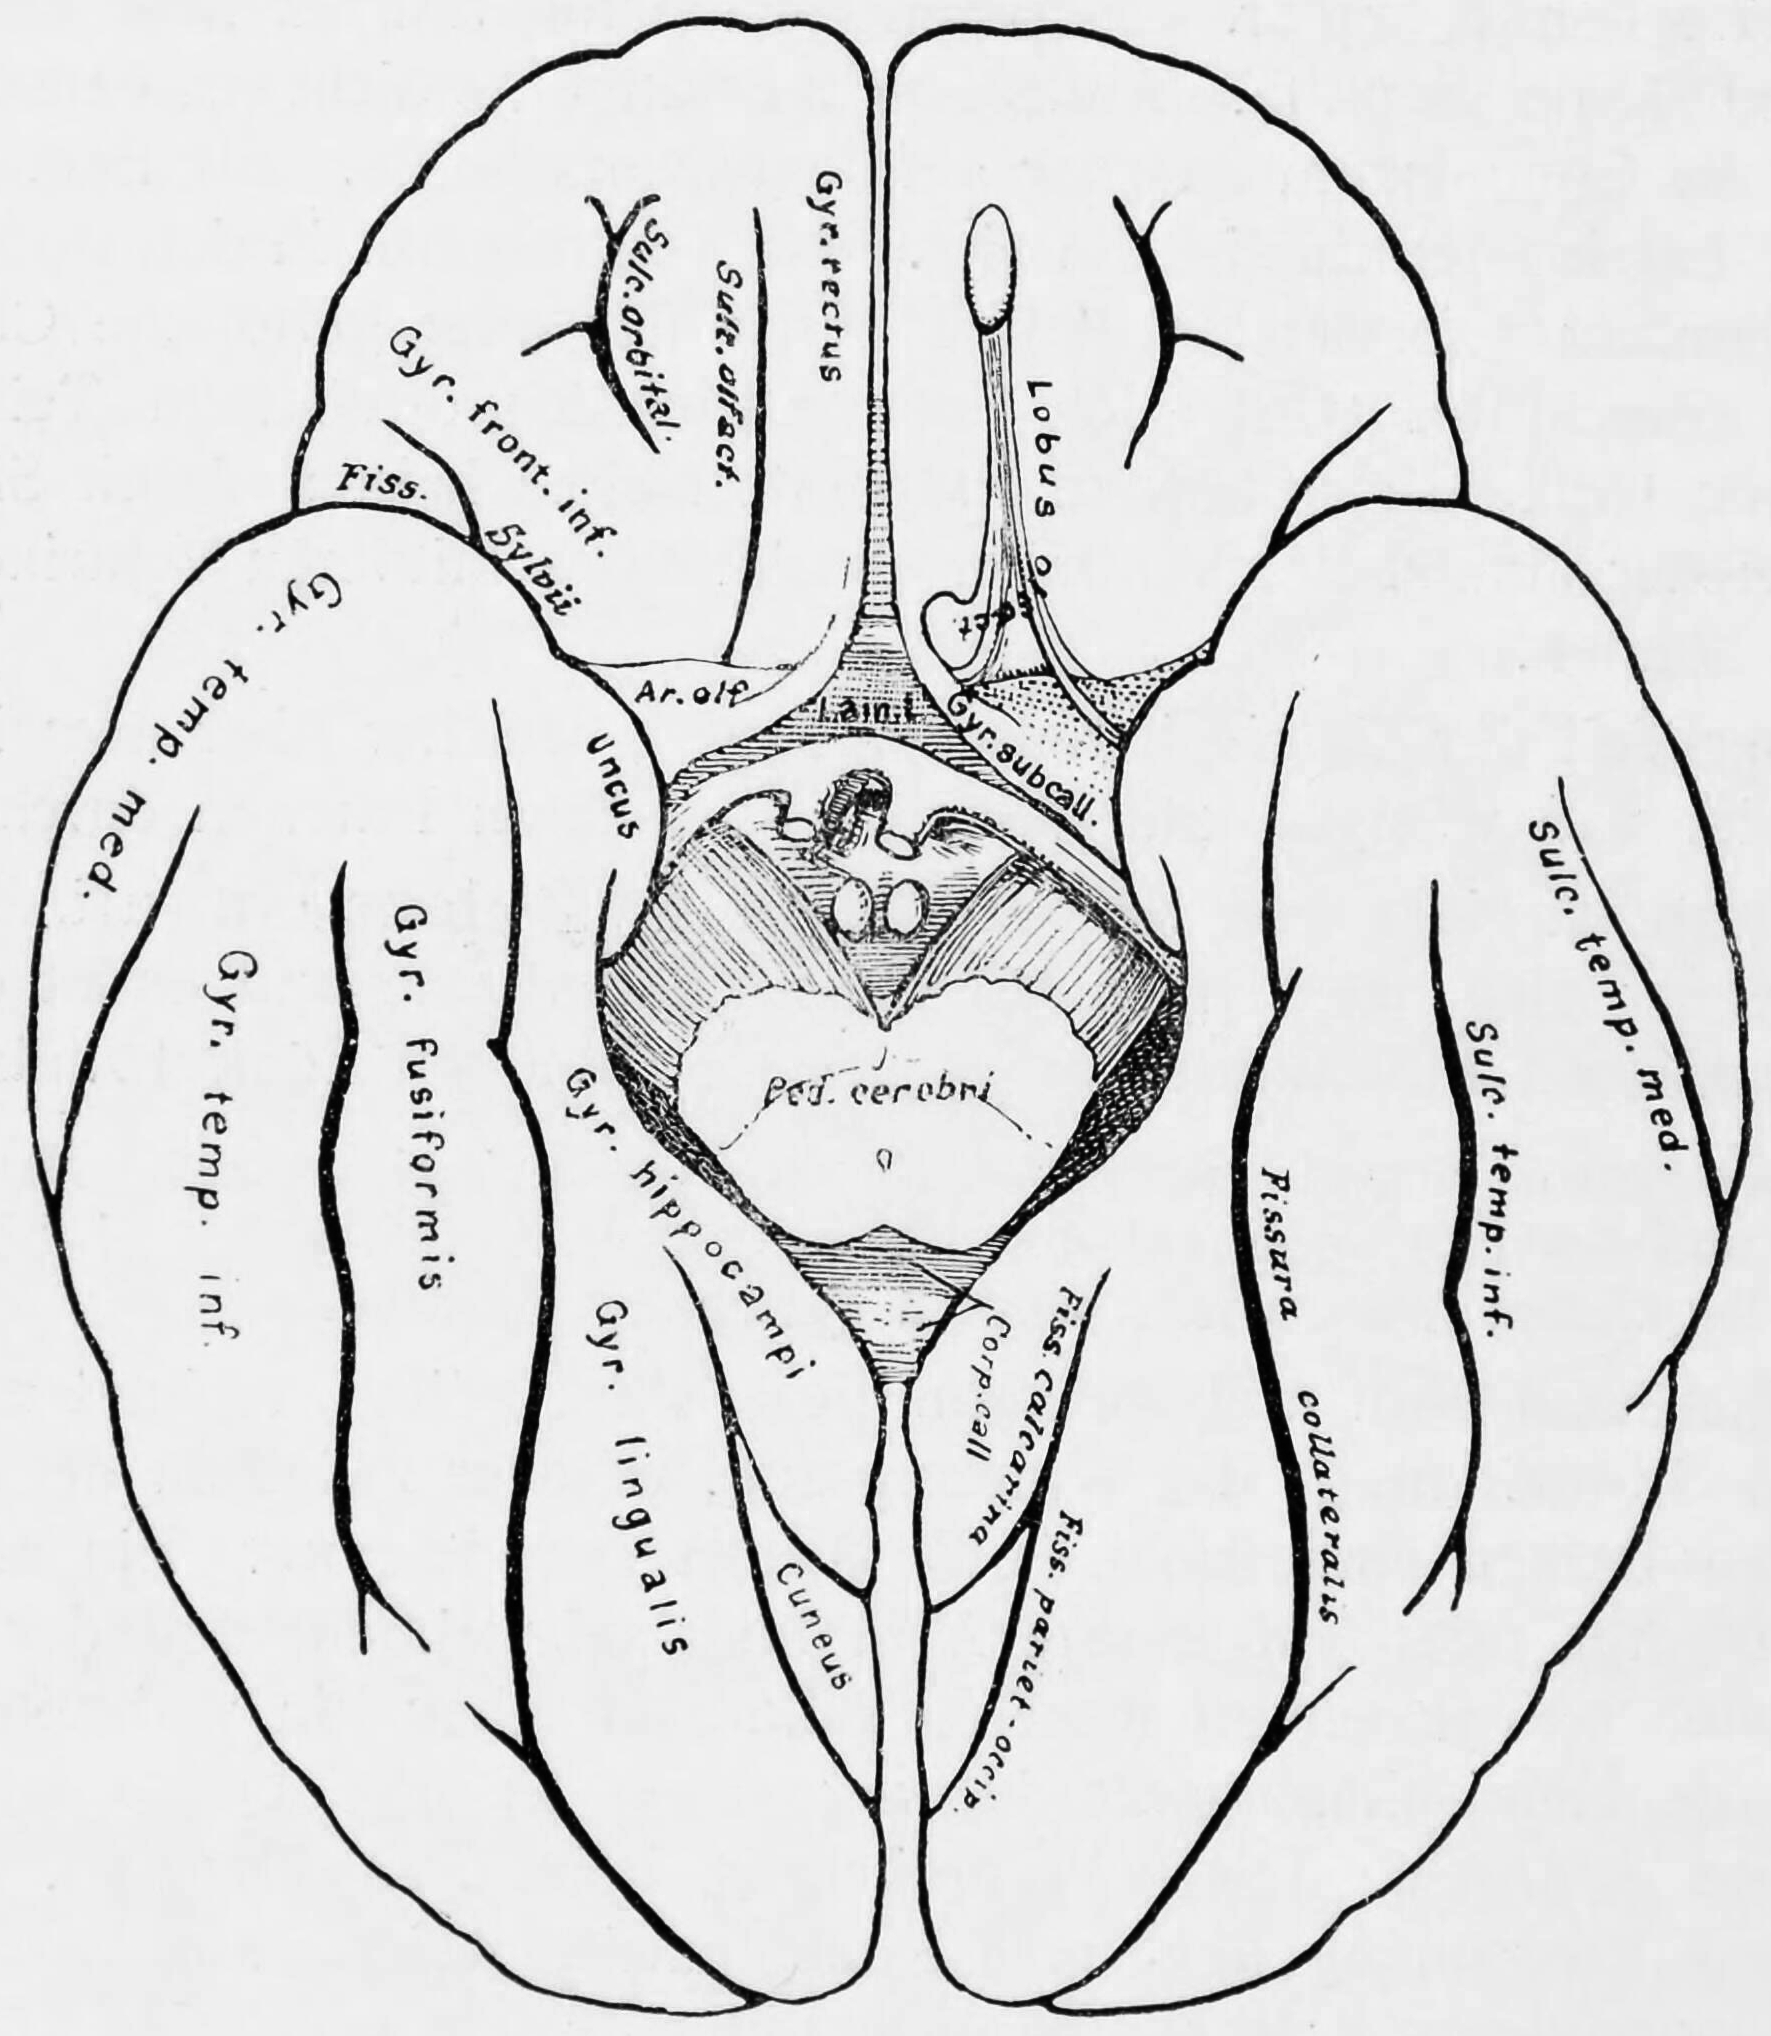
\includegraphics[width=0.7\linewidth]{./figures/nervoussystem/gyri_bot} 

}

\caption{Diagram showing a view from the bottom of the ridges (gyri) and grooves (sulci) of the left hemisphere of the brain.}\label{fig:gyribottom}
\end{figure}

Although the human brain represents only 2\% of the body weight, it receives 15\% of the cardiac output, 20\% of total body oxygen consumption, and 25\% of total body glucose utilization. The brain mostly uses glucose for energy, and deprivation of glucose, as can happen in hypoglycemia, can result in loss of consciousness. The energy consumption of the brain does not vary greatly over time, but active regions of the cortex consume somewhat more energy than inactive regions: this fact forms the basis for the functional brain imaging methods PET and fMRI. These functional imaging techniques provide a three-dimensional image of metabolic activity.

The simplest way to gain information about brain anatomy is by visual inspection, but many more sophisticated techniques have been developed. Brain tissue in its natural state is too soft to work with, but it can be hardened by immersion in alcohol or other fixatives, and then sliced apart for examination of the interior. Visually, the interior of the brain consists of areas of so-called grey matter, with a dark color, separated by areas of white matter, with a lighter color. Further information can be gained by staining slices of brain tissue with a variety of chemicals that bring out areas where specific types of molecules are present in high concentrations. It is also possible to examine the microstructure of brain tissue using a microscope, and to trace the pattern of connections from one brain area to another.

\hypertarget{development-of-the-nervous-system}{%
\section{Development Of The Nervous System}\label{development-of-the-nervous-system}}

All bilaterian animals at an early stage of development form a gastrula, which is polarized, with one end called the animal pole and the other the vegetal pole. The gastrula has the shape of a disk with three layers of cells, an inner layer called the endoderm, which gives rise to the lining of most internal organs, a middle layer called the mesoderm, which gives rise to the bones and muscles, and an outer layer called the ectoderm, which gives rise to the skin and nervous system.

In vertebrates, the first sign of the nervous system is the appearance of a thin strip of cells along the center of the back, called the neural plate. The inner portion of the neural plate (along the midline) is destined to become the central nervous system (CNS), the outer portion the peripheral nervous system (PNS). As development proceeds, a fold called the neural groove appears along the midline. This fold deepens, and then closes up at the top. At this point the future CNS appears as a cylindrical structure called the neural tube, whereas the future PNS appears as two strips of tissue called the neural crest, running lengthwise above the neural tube. The sequence of stages from neural plate to neural tube and neural crest is known as neurulation.

In the early 20\textsuperscript{th} century, a set of famous experiments by \href{https://en.wikipedia.org/wiki/Hans_Spemann}{Hans Spemann} and \href{https://en.wikipedia.org/wiki/Hilde_Mangold}{Hilde Mangold} showed that the formation of nervous tissue is ``induced'' by signals from a group of mesodermal cells called the organizer region. For decades, though, the nature of neural induction defeated every attempt to figure it out, until finally it was resolved by genetic approaches in the 1990s. Induction of neural tissue requires inhibition of the gene for a so-called bone morphogenetic protein, or BMP. Specifically the protein BMP4 appears to be involved. Two proteins called Noggin and Chordin, both secreted by the mesoderm, are capable of inhibiting BMP4 and thereby inducing ectoderm to turn into neural tissue. It appears that a similar molecular mechanism is involved for widely disparate types of animals, including arthropods as well as vertebrates. In some animals, however, another type of molecule called Fibroblast Growth Factor or FGF may also play an important role in induction.

Induction of neural tissues causes formation of neural precursor cells, called neuroblasts. In drosophila, neuroblasts divide asymmetrically, so that one product is a ``ganglion mother cell'' (GMC), and the other is a neuroblast. A GMC divides once, to give rise to either a pair of neurons or a pair of glial cells. In all, a neuroblast is capable of generating an indefinite number of neurons or glia.

One factor common to all bilateral organisms (including humans) is a family of secreted signaling molecules called neurotrophins which regulate the growth and survival of neurons. Because neurotrophins have now been identified in both vertebrate and invertebrates, this evidence suggests that neurotrophins were present in an ancestor common to bilateral organisms and may represent a common mechanism for nervous system formation.

\hypertarget{the-function-of-the-nervous-system}{%
\section{The Function Of The Nervous System}\label{the-function-of-the-nervous-system}}

Organisms need information to solve at least three kinds of problems: (a) to maintain an appropriate environment, i.e., homeostasis; (b) to time activities (e.g., seasonal changes in behavior) or synchronize activities with those of conspecifics; and (c) to locate and respond to resources or threats (e.g., by moving towards resources or evading or attacking threats). Organisms also need to transmit information in order to influence another's behavior: to identify themselves, warn conspecifics of danger, coordinate activities, or deceive.

At the most basic level, the function of the nervous system is to send signals from one cell to others, or from one part of the body to others. There are multiple ways that a cell can send signals to other cells. One is by releasing chemicals called hormones into the internal circulation, so that they can diffuse to distant sites. In contrast to this ``broadcast'' mode of signaling, the nervous system provides ``point-to-point'' signals---neurons project their axons to specific target areas and make synaptic connections with specific target cells. Thus, neural signaling is capable of a much higher level of specificity than hormonal signaling. It is also much faster: the fastest nerve signals travel at speeds that exceed 100 meters per second.

At a more integrative level, the primary function of the nervous system is to control the body. It does this by extracting information from the environment using sensory receptors, sending signals that encode this information into the central nervous system, processing the information to determine an appropriate response, and sending output signals to muscles or glands to activate the response. The evolution of a complex nervous system has made it possible for various animal species to have advanced perception abilities such as vision, complex social interactions, rapid coordination of organ systems, and integrated processing of concurrent signals. In humans, the sophistication of the nervous system makes it possible to have language, abstract representation of concepts, transmission of culture, and many other features of human society that would not exist without the human brain.

\hypertarget{the-sensory-system}{%
\section{The Sensory System}\label{the-sensory-system}}

The sensory nervous system is a part of the nervous system responsible for processing sensory information. A sensory system consists of sensory neurons (including the sensory receptor cells), neural pathways, and parts of the brain involved in sensory perception. Commonly recognized sensory systems are those for vision, hearing, touch, taste, smell, and balance. In short, senses are transducers from the physical world to the realm of the mind where we interpret the information, creating our perception of the world around us.

Sensory systems code for four aspects of a stimulus; type (modality), intensity, location, and duration. Arrival time of a sound pulse and phase differences of continuous sound are used for sound localization. Certain receptors are sensitive to certain types of stimuli (for example, different mechanoreceptors respond best to different kinds of touch stimuli, like sharp or blunt objects). Receptors send impulses in certain patterns to send information about the intensity of a stimulus (for example, how loud a sound is). The location of the receptor that is stimulated gives the brain information about the location of the stimulus (for example, stimulating a mechanoreceptor in a finger will send information to the brain about that finger). The duration of the stimulus (how long it lasts) is conveyed by firing patterns of receptors. These impulses are transmitted to the brain through afferent neurons.

While debate exists among neurologists as to the specific number of senses due to differing definitions of what constitutes a sense, Gautama Buddha and Aristotle classified five `traditional' human senses which have become universally accepted: touch, taste, smell, sight, and hearing. Other senses that have been well-accepted in most mammals, including humans, include nociception, equilibrioception, kinaesthesia, and thermoception. Furthermore, some nonhuman animals have been shown to possess alternate senses, including magnetoception and electroreception.

The human sensory system consists of the following subsystems:

\begin{itemize}
\tightlist
\item
  Somatosensory system consists of the receptors, transmitters (pathways) leading to area S1, and area S1 in the cortex that is involved in creating the conscious experience of the sensations labelled as touch or pressure, temperature (warm or cold), pain (including itch and tickle), and the sensations of muscle movement and joint position including posture, movement, and facial expression (collectively also called proprioception)
\item
  Visual system
\item
  Auditory system
\item
  Vestibular system
\item
  Olfactory system
\item
  Gustatory system
\end{itemize}

The receptive field is the area of the body or environment to which a receptor organ and receptor cells respond. For instance, the part of the world an eye can see, is its receptive field; the light that each rod or cone can see, is its receptive field. Receptive fields have been identified for the visual system, auditory system and somatosensory system.

\hypertarget{the-motor-system}{%
\section{The Motor System}\label{the-motor-system}}

The motor system is the set of central and peripheral structures in the nervous system that support motor functions, i.e.~movement. Peripheral structures may include skeletal muscles and neural connections with muscle tissues. Central structures include cerebral cortex, brainstem, spinal cord, pyramidal system including the upper motor neurons, extrapyramidal system, cerebellum, and the lower motor neurons in the brainstem and the spinal cord.

The pyramidal motor system, also called the pyramidal tract or the corticospinal tract, start in the motor center of the cerebral cortex. There are upper and lower motor neurons in the corticospinal tract. The motor impulses originate in the giant pyramidal cells or Betz cells of the motor area; i.e., precentral gyrus of cerebral cortex. These are the upper motor neurons (UMN) of the corticospinal tract. The axons of these cells pass in the depth of the cerebral cortex to the corona radiata and then to the internal capsule passing through the posterior branch of internal capsule and continue to descend in the midbrain and the medulla oblongata. In the lower part of medulla oblongata 80 to 85\% of these fibers decussate (pass to the opposite side) and descend in the white matter of the lateral funiculus of the spinal cord on the opposite side. The remaining 15 to 20\% pass to the same side. Fibers for the extremities (limbs) pass 100\% to the opposite side. The fibers of the corticospinal tract terminate at different levels in the anterior horn of the grey matter of the spinal cord. Here the lower motor neurons (LMN) of the spinal cord are located. Peripheral motor nerves carry the motor impulses from the anterior horn to the voluntary muscles.

The extrapyramidal system is called extrapyramidal to distinguish it from the tracts of the motor cortex that reach their targets by traveling through the pyramids of the medulla. The pyramidal tracts (corticospinal tract and corticobulbar tracts) may directly innervate motor neurons of the spinal cord or brainstem (anterior (ventral) horn cells or certain cranial nerve nuclei), whereas the extrapyramidal system centers on the modulation and regulation (indirect control) of anterior (ventral) horn cells.

Extrapyramidal tracts are chiefly found in the reticular formation of the pons and medulla, and target lower motor neurons in the spinal cord that are involved in reflexes, locomotion, complex movements, and postural control. These tracts are in turn modulated by various parts of the central nervous system, including the nigrostriatal pathway, the basal ganglia, the cerebellum, the vestibular nuclei, and different sensory areas of the cerebral cortex. All of these regulatory components can be considered part of the extrapyramidal system, in that they modulate motor activity without directly innervating motor neurons.

\hypertarget{neuronal-signalling}{%
\section{Neuronal Signalling}\label{neuronal-signalling}}

Most neurons send signals via their axons, although some types are capable of dendrite-to-dendrite communication. (In fact, the types of neurons in the retina of the eye called amacrine cells have no axons, and communicate only via their dendrites.) Neural signals propagate along an axon in the form of electrochemical waves called action potentials, which produce cell-to-cell signals at points where axon terminals make synaptic contact with other cells.

Synapses may be electrical or chemical. Electrical synapses make direct electrical connections between neurons, but chemical synapses are much more common, and much more diverse in function. At a chemical synapse, the cell that sends signals is called presynaptic, and the cell that receives signals is called postsynaptic. Both the presynaptic and postsynaptic areas are full of molecular machinery that carries out the signalling process. The presynaptic area contains large numbers of tiny spherical vessels called synaptic vesicles, packed with neurotransmitter chemicals. When the presynaptic terminal is electrically stimulated, an array of molecules embedded in the membrane are activated, and cause the contents of the vesicles to be released into the narrow space between the presynaptic and postsynaptic membranes, called the synaptic cleft. The neurotransmitter then binds to receptors embedded in the postsynaptic membrane, causing them to enter an activated state. Depending on the type of receptor, the resulting effect on the postsynaptic cell may be excitatory, inhibitory, or modulatory in more complex ways. For example, release of the neurotransmitter acetylcholine at a synaptic contact between a motor neuron and a muscle cell induces rapid contraction of the muscle cell. The entire synaptic transmission process takes only a fraction of a millisecond, although the effects on the postsynaptic cell may last much longer (even indefinitely, in cases where the synaptic signal leads to the formation of a memory trace).

There are literally hundreds of different types of synapses. In fact, there are over a hundred known neurotransmitters, and many of them have multiple types of receptors. Many synapses use more than one neurotransmitter---a common arrangement is for a synapse to use one fast-acting small-molecule neurotransmitter such as glutamate or GABA, along with one or more peptide neurotransmitters that play slower-acting modulatory roles. Molecular neuroscientists generally divide receptors into two broad groups: chemically gated ion channels and second messenger systems. When a chemically gated ion channel is activated, it forms a passage that allows specific types of ions to flow across the membrane. Depending on the type of ion, the effect on the target cell may be excitatory or inhibitory. When a second messenger system is activated, it starts a cascade of molecular interactions inside the target cell, which may ultimately produce a wide variety of complex effects, such as increasing or decreasing the sensitivity of the cell to stimuli, or even altering gene transcription.

According to a rule called Dale's principle, which has only a few known exceptions, a neuron releases the same neurotransmitters at all of its synapses. This does not mean, though, that a neuron exerts the same effect on all of its targets, because the effect of a synapse depends not on the neurotransmitter, but on the receptors that it activates. Because different targets can (and frequently do) use different types of receptors, it is possible for a neuron to have excitatory effects on one set of target cells, inhibitory effects on others, and complex modulatory effects on others still. Nevertheless, it happens that the two most widely used neurotransmitters, glutamate and GABA, each have largely consistent effects. Glutamate has several widely occurring types of receptors, but all of them are excitatory or modulatory. Similarly, GABA has several widely occurring receptor types, but all of them are inhibitory. Because of this consistency, glutamatergic cells are frequently referred to as ``excitatory neurons'', and GABAergic cells as ``inhibitory neurons''. Strictly speaking, this is an abuse of terminology---it is the receptors that are excitatory and inhibitory, not the neurons---but it is commonly seen even in scholarly publications.

One very important subset of synapses are capable of forming memory traces by means of long-lasting activity-dependent changes in synaptic strength. The best-known form of neural memory is a process called long-term potentiation (abbreviated LTP), which operates at synapses that use the neurotransmitter glutamate acting on a special type of receptor known as the NMDA receptor. The NMDA receptor functions as a molecular ``conincidence detector'': although the NMDA-receptor associated ion-channel opens upon binding of glutamate, extracellular Mg\textsuperscript{2+} ions will enter and block the channel immediately. Only concomitant membrane depolarization (e.g.~induced by Na\textsuperscript{+} influx via concomittantly stimulated non-NMDA (AMPA) type glutamate receptors in the same cell), will overcome the Mg\textsuperscript{2+} block and allow Na\textsuperscript{+} and Ca\textsuperscript{2+} ions to enter the cell thourgh the NMDA-receptor. Calcium entering the postsynaptic cell via NMDA receptors then initiates a second messenger cascade that ultimately leads to an increase in the number of AMPA-type glutamate receptors in the target cell, thereby increasing the effective strength of the synapse. This change in strength can last for weeks or longer. Since the discovery of LTP in 1973, many other types of synaptic memory traces have been found, involving increases or decreases in synaptic strength that are induced by varying conditions, and last for variable periods of time. The reward system, that reinforces desired behaviour for example, depends on a variant form of LTP that is conditioned on an extra input coming from a reward-signalling pathway that uses dopamine as neurotransmitter. All these forms of synaptic modifiability, taken collectively, give rise to neural plasticity, that is, to a capability for the nervous system to adapt itself to variations in the environment.

\hypertarget{neural-circuits}{%
\section{Neural Circuits}\label{neural-circuits}}

The basic neuronal function of sending signals to other cells includes a capability for neurons to exchange signals with each other. Networks formed by interconnected groups of neurons are capable of a wide variety of functions, including feature detection, pattern generation and timing, and there are seen to be countless types of information processing possible. \href{https://en.wikipedia.org/wiki/Warren_Sturgis_McCulloch}{Warren McCulloch} and \href{https://en.wikipedia.org/wiki/Walter_Pitts}{Walter Pitts} showed in 1943 that even artificial neural networks formed from a greatly simplified mathematical abstraction of a neuron are capable of universal computation.

Historically, for many years the predominant view of the function of the nervous system was as a stimulus-response associator. In this conception, neural processing begins with stimuli that activate sensory neurons, producing signals that propagate through chains of connections in the spinal cord and brain, giving rise eventually to activation of motor neurons and thereby to muscle contraction, i.e., to overt responses. The French philosopher \href{https://en.wikipedia.org/wiki/René_Descartes}{René Descartes} believed that all of the behaviors of animals, and most of the behaviors of humans, could be explained in terms of stimulus-response circuits, although he also believed that higher cognitive functions such as language were not capable of being explained mechanistically. \href{https://en.wikipedia.org/wiki/Charles_Scott_Sherrington}{Charles Sherrington}, in his influential 1906 book The Integrative Action of the Nervous System, developed the concept of stimulus-response mechanisms in much more detail, and Behaviorism, the school of thought that dominated Psychology through the middle of the 20\textsuperscript{th} century, attempted to explain every aspect of human behavior in stimulus-response terms.

However, experimental studies of electrophysiology, beginning in the early 20\textsuperscript{th} century and reaching high productivity by the 1940s, showed that the nervous system contains many mechanisms for generating patterns of activity intrinsically, without requiring an external stimulus. Neurons were found to be capable of producing regular sequences of action potentials, or sequences of bursts, even in complete isolation. When intrinsically active neurons are connected to each other in complex circuits, the possibilities for generating intricate temporal patterns become far more extensive. A modern conception views the function of the nervous system partly in terms of stimulus-response chains, and partly in terms of intrinsically generated activity patterns---both types of activity interact with each other to generate the full repertoire of behavior.

\hypertarget{reflexes-and-other-stimulus-response-circuits}{%
\section{Reflexes And Other Stimulus-Response Circuits}\label{reflexes-and-other-stimulus-response-circuits}}

The simplest type of neural circuit is a reflex arc, which begins with a sensory input and ends with a motor output, passing through a sequence of neurons connected in series. This can be shown in the ``withdrawal reflex'' causing a hand to jerk back after a hot stove is touched. The circuit begins with sensory receptors in the skin that are activated by harmful levels of heat: a special type of molecular structure embedded in the membrane causes heat to change the electrical field across the membrane. If the change in electrical potential is large enough to pass the given threshold, it evokes an action potential, which is transmitted along the axon of the receptor cell, into the spinal cord. There the axon makes excitatory synaptic contacts with other cells, some of which project (send axonal output) to the same region of the spinal cord, others projecting into the brain. One target is a set of spinal interneurons that project to motor neurons controlling the arm muscles. The interneurons excite the motor neurons, and if the excitation is strong enough, some of the motor neurons generate action potentials, which travel down their axons to the point where they make excitatory synaptic contacts with muscle cells. The excitatory signals induce contraction of the muscle cells, which causes the joint angles in the arm to change, pulling the arm away.

In reality, this straightforward schema is subject to numerous complications. Although for the simplest reflexes there are short neural paths from sensory neuron to motor neuron, there are also other nearby neurons that participate in the circuit and modulate the response. Furthermore, there are projections from the brain to the spinal cord that are capable of enhancing or inhibiting the reflex.

Although the simplest reflexes may be mediated by circuits lying entirely within the spinal cord, more complex responses rely on signal processing in the brain. For example, when an object in the periphery of the visual field moves, and a person looks toward it many stages of signal processing are initiated. The initial sensory response, in the retina of the eye, and the final motor response, in the oculomotor nuclei of the brain stem, are not all that different from those in a simple reflex, but the intermediate stages are completely different. Instead of a one or two step chain of processing, the visual signals pass through perhaps a dozen stages of integration, involving the thalamus, cerebral cortex, basal ganglia, superior colliculus, cerebellum, and several brainstem nuclei. These areas perform signal-processing functions that include feature detection, perceptual analysis, memory recall, decision-making, and motor planning.

Feature detection is the ability to extract biologically relevant information from combinations of sensory signals. In the visual system, for example, sensory receptors in the retina of the eye are only individually capable of detecting ``points of light'' in the outside world. Second-level visual neurons receive input from groups of primary receptors, higher-level neurons receive input from groups of second-level neurons, and so on, forming a hierarchy of processing stages. At each stage, important information is extracted from the signal ensemble and unimportant information is discarded. By the end of the process, input signals representing ``points of light'' have been transformed into a neural representation of objects in the surrounding world and their properties. The most sophisticated sensory processing occurs inside the brain, but complex feature extraction also takes place in the spinal cord and in peripheral sensory organs such as the retina.

\hypertarget{intrinsic-pattern-generation}{%
\section{Intrinsic Pattern Generation}\label{intrinsic-pattern-generation}}

Although stimulus-response mechanisms are the easiest to understand, the nervous system is also capable of controlling the body in ways that do not require an external stimulus, by means of internally generated rhythms of activity. Because of the variety of voltage-sensitive ion channels that can be embedded in the membrane of a neuron, many types of neurons are capable, even in isolation, of generating rhythmic sequences of action potentials, or rhythmic alternations between high-rate bursting and quiescence. When neurons that are intrinsically rhythmic are connected to each other by excitatory or inhibitory synapses, the resulting networks are capable of a wide variety of dynamical behaviors, including attractor dynamics, periodicity, and even chaos. A network of neurons that uses its internal structure to generate temporally structured output, without requiring a corresponding temporally structured stimulus, is called a central pattern generator.

Internal pattern generation operates on a wide range of time scales, from milliseconds to hours or longer. One of the most important types of temporal pattern is circadian rhythmicity---that is, rhythmicity with a period of approximately 24 hours. All animals that have been studied show circadian fluctuations in neural activity, which control circadian alternations in behavior such as the sleep-wake cycle. Experimental studies dating from the 1990s have shown that circadian rhythms are generated by a ``genetic clock'' consisting of a special set of genes whose expression level rises and falls over the course of the day. Animals as diverse as insects and vertebrates share a similar genetic clock system. The circadian clock is influenced by light but continues to operate even when light levels are held constant and no other external time-of-day cues are available. The clock genes are expressed in many parts of the nervous system as well as many peripheral organs, but in mammals, all of these ``tissue clocks'' are kept in synchrony by signals that emanate from a master timekeeper in a tiny part of the brain called the suprachiasmatic nucleus.

\hypertarget{development-of-the-nervous-system-1}{%
\chapter{Development Of The Nervous System}\label{development-of-the-nervous-system-1}}

The development of the nervous system, or neural development, or neurodevelopment, refers to the processes that generate, shape, and reshape the nervous system of animals, from the earliest stages of embryonic development to adulthood. The field of neural development draws on both neuroscience and developmental biology to describe and provide insight into the cellular and molecular mechanisms by which complex nervous systems develop, from nematodes and fruit flies to mammals. Defects in neural development can lead to malformations and a wide variety of sensory, motor, and cognitive impairments neurological disorders and intellectual disability.

The central nervous system (CNS) is derived from the ectoderm---the outermost tissue layer of the embryo. In the third week of human embryonic development the neuroectoderm appears and forms the neural plate along the dorsal side of the embryo. The neural plate is the source of the majority of neurons and glial cells of the CNS. A groove forms along the long axis of the neural plate and, by week four of development, the neural plate wraps in on itself to give rise to the neural tube, which is filled with cerebrospinal fluid (CSF).

As the embryo develops, the anterior part of the neural tube forms three primary brain vesicles, which become the primary anatomical regions of the brain: the forebrain (prosencephalon), midbrain (mesencephalon), and hindbrain (rhombencephalon). These simple, early vesicles enlarge and further divide into the five secondary brain vesicles -- the telencephalon (future cerebral cortex and basal ganglia), diencephalon (future thalamus and hypothalamus), mesencephalon (future colliculi), metencephalon (future pons and cerebellum), and myelencephalon (future medulla). The CSF-filled central chamber is continuous from the telencephalon to the spinal cord, and constitutes the developing ventricular system of the CNS. Because the neural tube gives rise to the brain and spinal cord any mutations at this stage in development can lead to fatal deformities like anencephaly or lifelong disabilities like spina bifida. During this time, the walls of the neural tube contain neural stem cells, which drive brain growth as they divide many times. Gradually some of the cells stop dividing and differentiate into neurons and glial cells, which are the main cellular components of the CNS. The newly generated neurons migrate to different parts of the developing brain to self-organize into different brain structures. Once the neurons have reached their regional positions, they extend axons and dendrites, which allow them to communicate with other neurons via synapses. Synaptic communication between neurons leads to the establishment of functional neural circuits that mediate sensory and motor processing, and underlie behavior.



\begin{figure}

{\centering 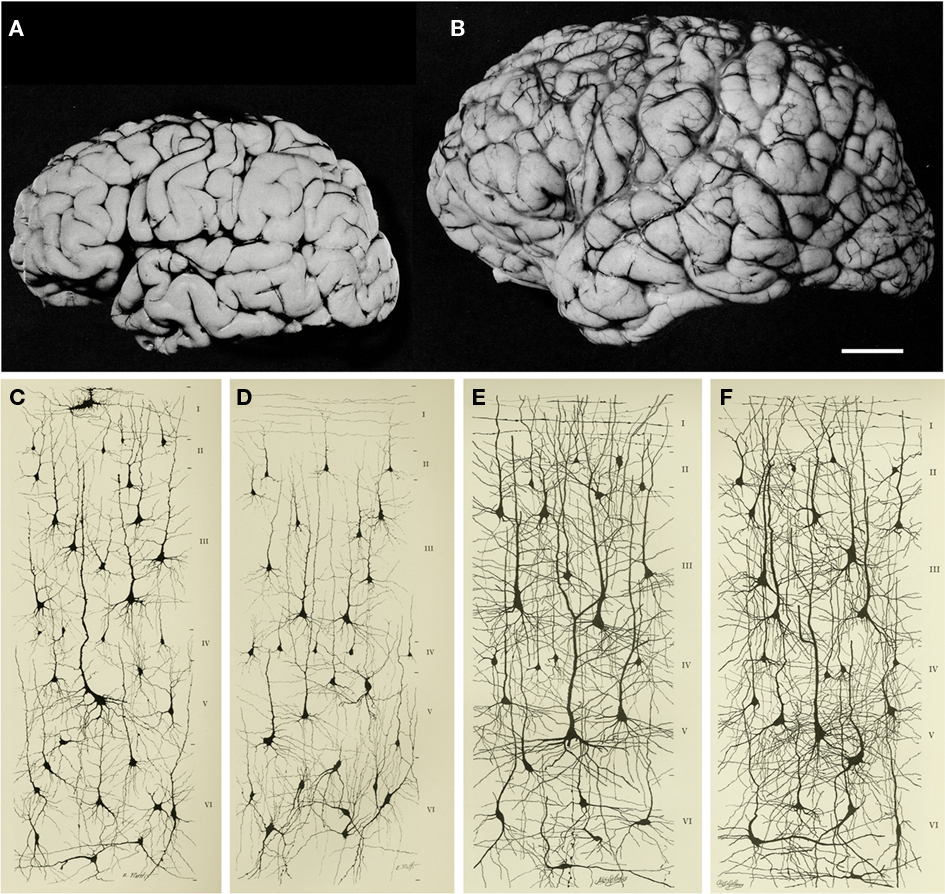
\includegraphics[width=0.7\linewidth]{./figures/development/fnana-05-00029-g004} 

}

\caption{Increase in brain size and the maturation of cortical circuits. The maturation of mental processes and motor skills is associated with an approximately fourfold enlargement in brain size. (A,B) photographs of the brains of a 1-month and 6-year-old-child. This increment is accompanied by a dramatic development in the complexity of the neuronal processes, which in turn is influenced by the genetic background and the environment. This increase in the complexity is clearly evident in the drawings of Golgi stained cortical neurons from the cerebral cortex of a 1-month {[}(C) ``pars triangularis of gyrus frontalis inferior''; (D) ``orbital gyrus''{]} and 6 year {[}(e), ``pars triangularis of gyrus frontalis inferior''; (F) ``orbital gyrus''{]} old child. Adapted from Conel and Le (1941, 1967). Scale bar for (A,B): 2 cm. From \href{https://www.frontiersin.org/article/10.3389/fnana.2011.00029}{DeFelipe J (2011) The evolution of the brain, the human nature of cortical circuits, and intellectual creativity. Front. Neuroanat. 5:29}}\label{fig:brainsize}
\end{figure}

\hypertarget{neural-induction}{%
\section{Neural Induction}\label{neural-induction}}

During early embryonic development the ectoderm becomes specified to give rise to the epidermis (skin) and the neural plate. The conversion of undifferentiated ectoderm to neuro-ectoderm requires signals from the mesoderm. At the onset of gastrulation presumptive mesodermal cells move through the dorsal blastopore lip and form a layer in between the endoderm and the ectoderm. These mesodermal cells that migrate along the dorsal midline give rise to a structure called the notochord. Ectodermal cells overlying the notochord develop into the neural plate in response to a diffusible signal produced by the notochord. The remainder of the ectoderm gives rise to the epidermis (skin). The ability of the mesoderm to convert the overlying ectoderm into neural tissue is called neural induction.

The neural plate folds outwards during the third week of gestation to form the neural groove. Beginning in the future neck region, the neural folds of this groove close to create the neural tube. The formation of the neural tube from the ectoderm is called neurulation. The ventral part of the neural tube is called the basal plate; the dorsal part is called the alar plate. The hollow interior is called the neural canal. By the end of the fourth week of gestation, the open ends of the neural tube, called the neuropores, close off.



\begin{figure}

{\centering 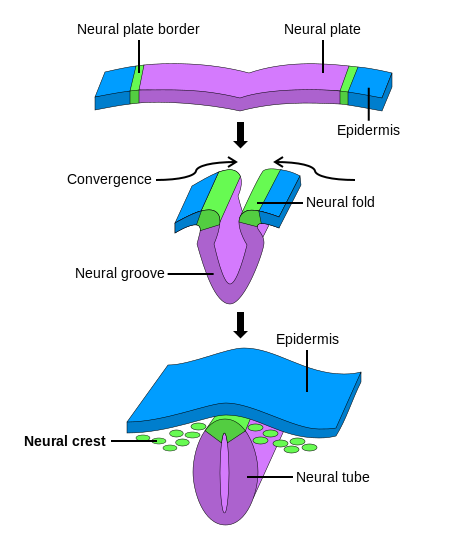
\includegraphics[width=0.7\linewidth]{./figures/development/neurulation} 

}

\caption{\href{https://en.wikipedia.org/wiki/Neural_tube\#/media/File:Neural_crest.svg}{A diagram of the stages of neural tube formation.}}\label{fig:neurulation}
\end{figure}

A transplanted blastopore lip can convert ectoderm into neural tissue and is said to have an inductive effect. Neural inducers are molecules that can induce the expression of neural genes in ectoderm explants without inducing mesodermal genes as well. Neural induction is often studied in \emph{Xenopus laevis} embryos since they have a simple body pattern and there are good markers to distinguish between neural and non-neural tissue. Examples of neural inducers are the molecules noggin and chordin.

When embryonic ectodermal cells are cultured at low density in the absence of mesodermal cells they undergo neural differentiation (express neural genes), suggesting that neural differentiation is the default fate of ectodermal cells. In explant cultures (which allow direct cell-cell interactions) the same cells differentiate into epidermis. This is due to the action of BMP4 (a TGF-β family protein) that induces ectodermal cultures to differentiate into epidermis. During neural induction, noggin and chordin are produced by the dorsal mesoderm (notochord) and diffuse into the overlying ectoderm to inhibit the activity of BMP4. This inhibition of BMP4 causes the cells to differentiate into neural cells. Inhibition of TGF-β and BMP (bone morphogenetic protein) signaling can efficiently induce neural tissue from human pluripotent stem cells, a model of early human development.

\hypertarget{the-early-brain}{%
\section{The Early Brain}\label{the-early-brain}}

Late in the fourth week, the superior part of the neural tube flexes at the level of the future midbrain---the mesencephalon. Above the mesencephalon is the prosencephalon (future forebrain) and beneath it is the rhombencephalon (future hindbrain). The optical vesicle (which will eventually become the optic nerve, retina and iris) forms at the basal plate of the prosencephalon.



\begin{figure}

{\centering \includegraphics[width=0.7\linewidth]{./figures/development/envhper00312-0143page3} 

}

\caption{Development of the mammalian brain. (A) and (B) The development of the three primary brain vesicles on gestational day (GD) 10.5 in rats and GD 26± 1 in humans.The corresponding shading between panels illustrates the earlier origins of different regions from the three original brain vesicles with horizontal and lateral views, respectively. (C) and (D) The more mature brain with five brain vesicles: the horizontal and lateral views correspond to GD11.5 in rats and GD 33 ± 1 in humans. (E) The lateral view shows the migratory paths from the more central ventricularzone and gradients maturation of the neocortex (arrows). (F) The midsagittal view of the brain and spinalcord, with the major divisions delineated and the continuity of the ventricles noted; the formation of the choroid plexus corresponds to GD 13.5 in rats and GD 48-51 in humans. Adapted from \href{https://www.ncbi.nlm.nih.gov/pubmed/10852851}{Rice and Barone}.}\label{fig:braindevelopment}
\end{figure}

The spinal cord forms from the lower part of the neural tube. The wall of the neural tube consists of neuroepithelial cells, which differentiate into neuroblasts, forming the mantle layer (the gray matter). Nerve fibers emerge from these neuroblasts to form the marginal layer (the white matter). The ventral part of the mantle layer (the basal plates) forms the motor areas of the spinal cord, whilst the dorsal part (the alar plates) forms the sensory areas. Between the basal and alar plates is an intermediate layer that contains neurons of the autonomic nervous system.



\begin{figure}

{\centering 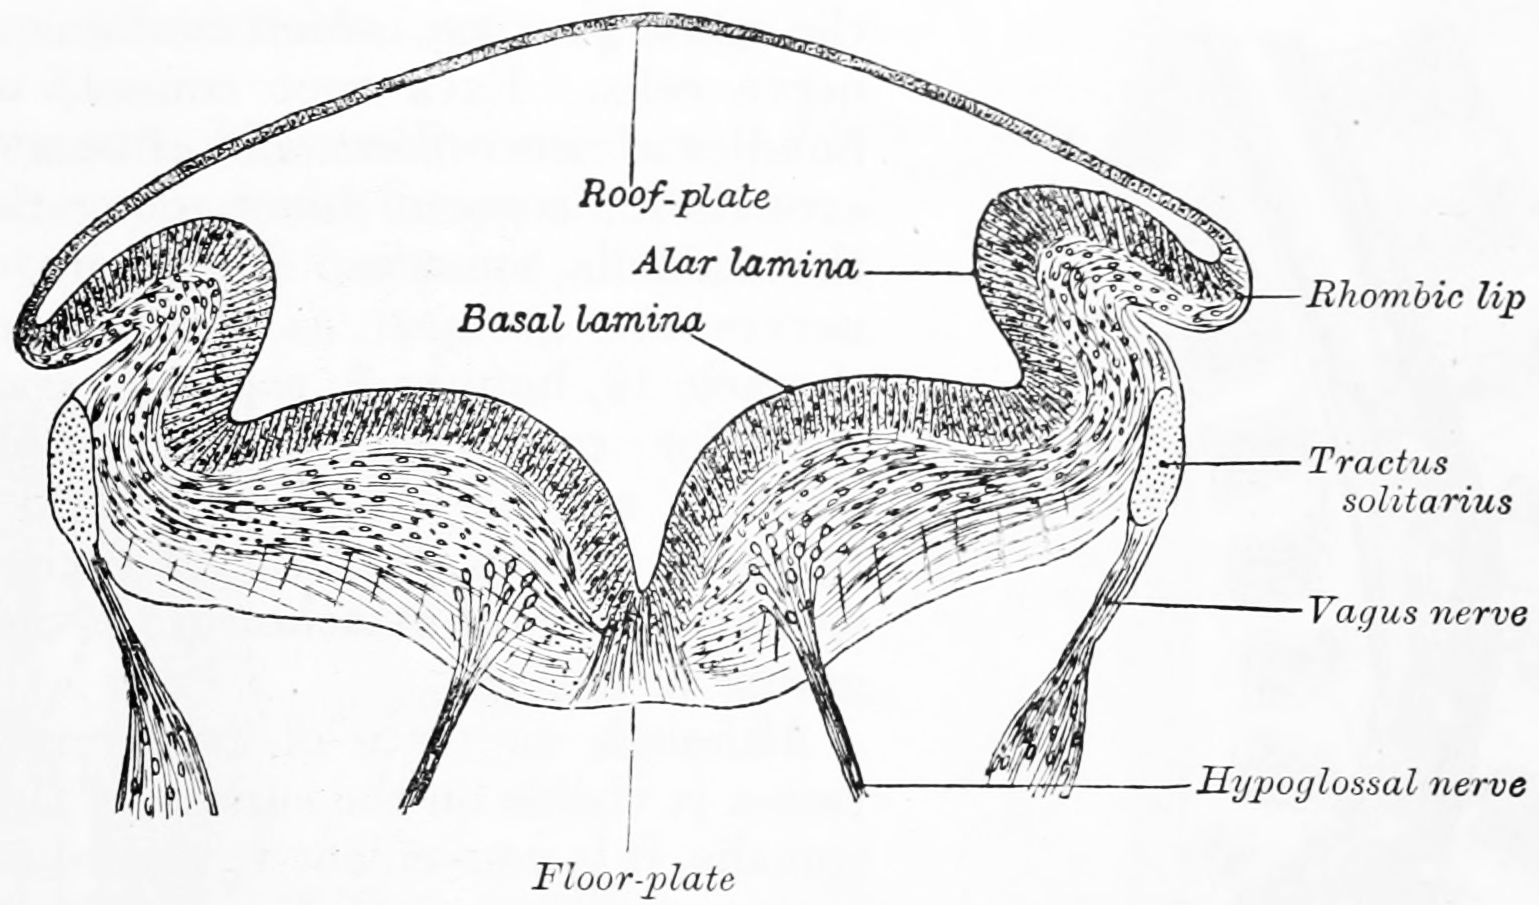
\includegraphics[width=0.7\linewidth]{./figures/development/GrayAnat1918p749} 

}

\caption{Transverse section of medulla oblongata of human embryo. From \href{https://archive.org/details/anatomyofhumanbo1918gray/page/n6/mode/2up}{Gray Henry, Anatomy of the Human Body. 20\textsuperscript{th} Edition, Lea \& Febiger, Philadelphia \& New York, 1918}}\label{fig:medullaoblongata}
\end{figure}

In the fifth week, the alar plate of the prosencephalon expands to form the cerebral hemispheres (the telencephalon). The basal plate becomes the diencephalon.



\begin{figure}

{\centering 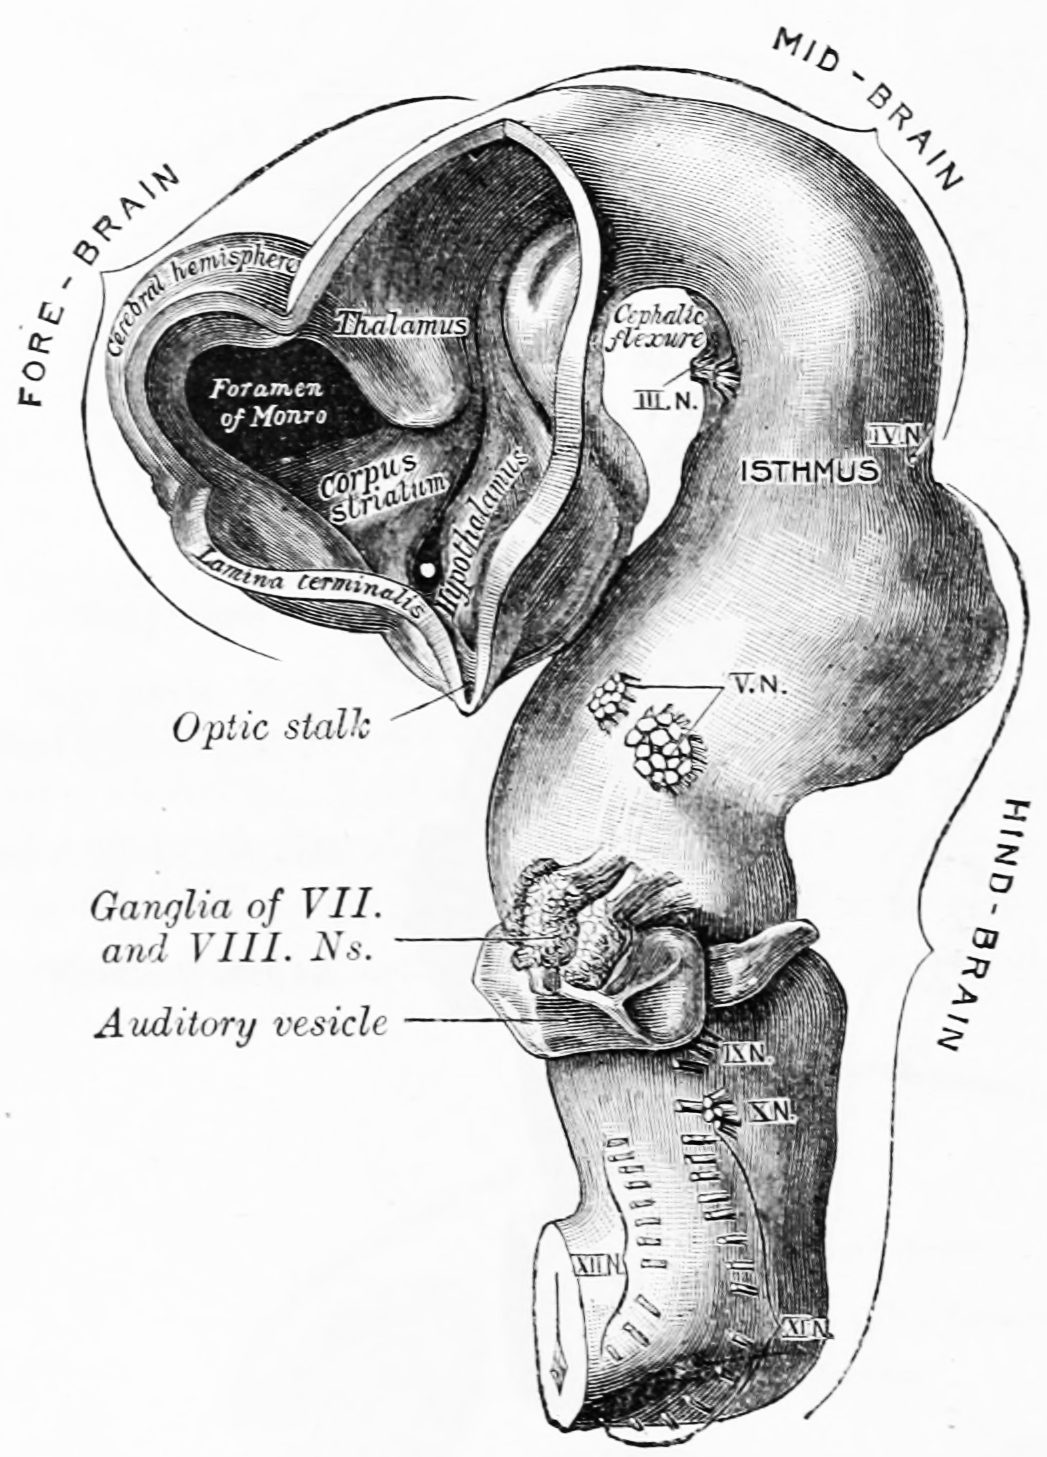
\includegraphics[width=0.7\linewidth]{./figures/development/GrayAnat1918p740} 

}

\caption{Brain of human embryo of four and a half weeks, showing interior of forebrain. From \href{https://archive.org/details/anatomyofhumanbo1918gray/page/n6/mode/2up}{Gray Henry, Anatomy of the Human Body. 20\textsuperscript{th} Edition, Lea \& Febiger, Philadelphia \& New York, 1918}}\label{fig:fourandahalf}
\end{figure}



\begin{figure}

{\centering 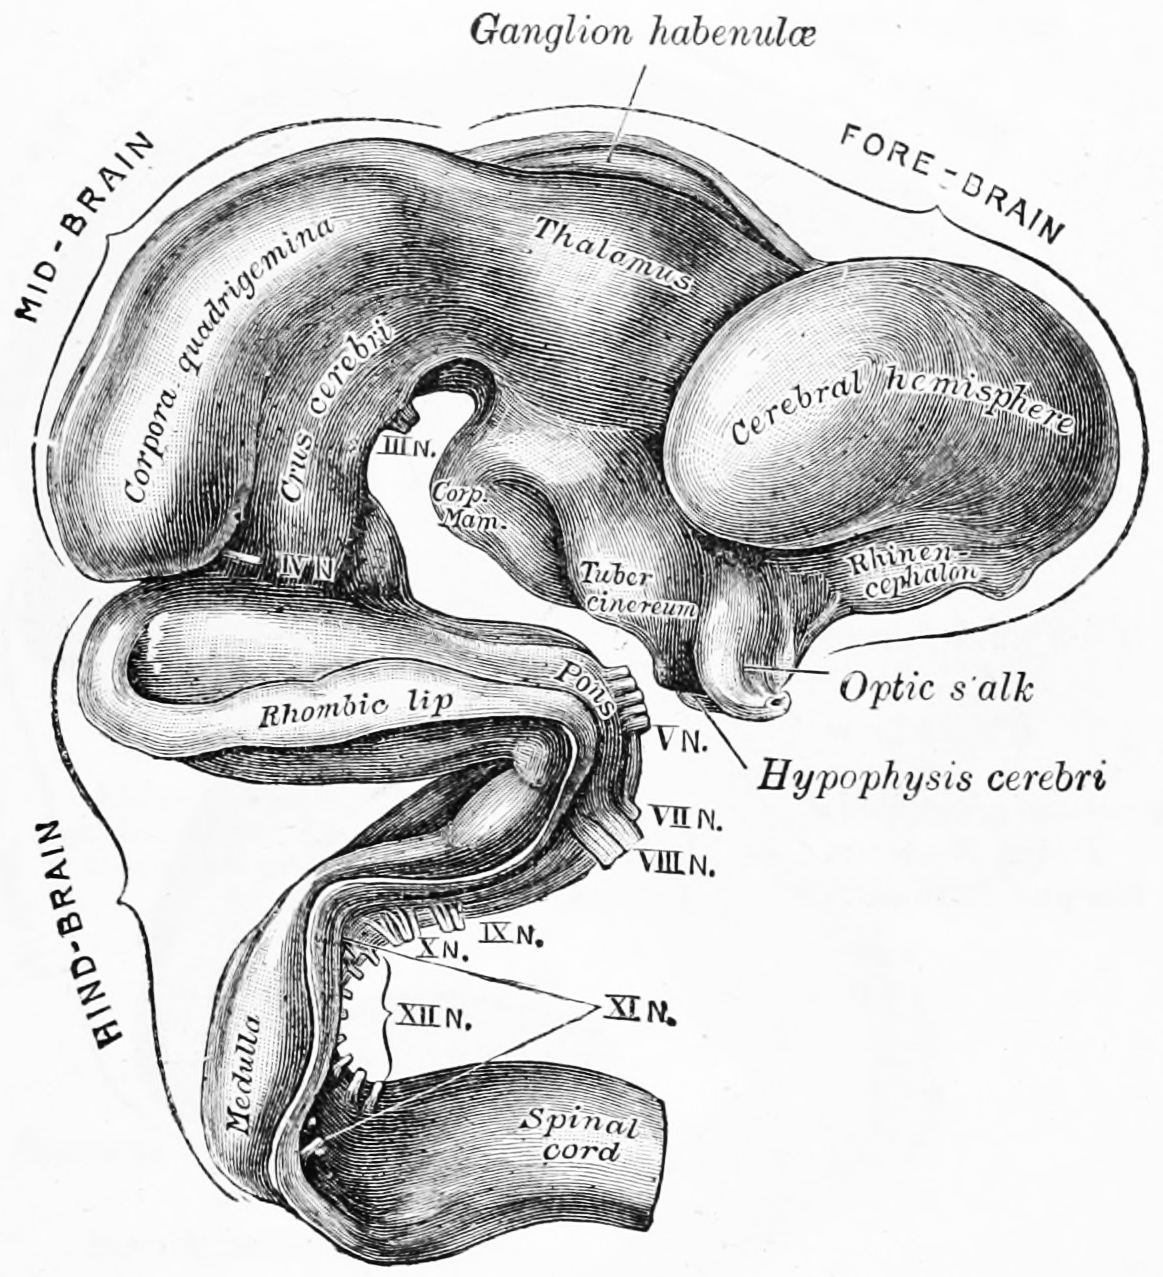
\includegraphics[width=0.7\linewidth]{./figures/development/GrayAnat1918p741} 

}

\caption{Exterior of brain of human embryo of five weeks. From \href{https://archive.org/details/anatomyofhumanbo1918gray/page/n6/mode/2up}{Gray Henry, Anatomy of the Human Body. 20\textsuperscript{th} Edition, Lea \& Febiger, Philadelphia \& New York, 1918}}\label{fig:fivexterior}
\end{figure}



\begin{figure}

{\centering 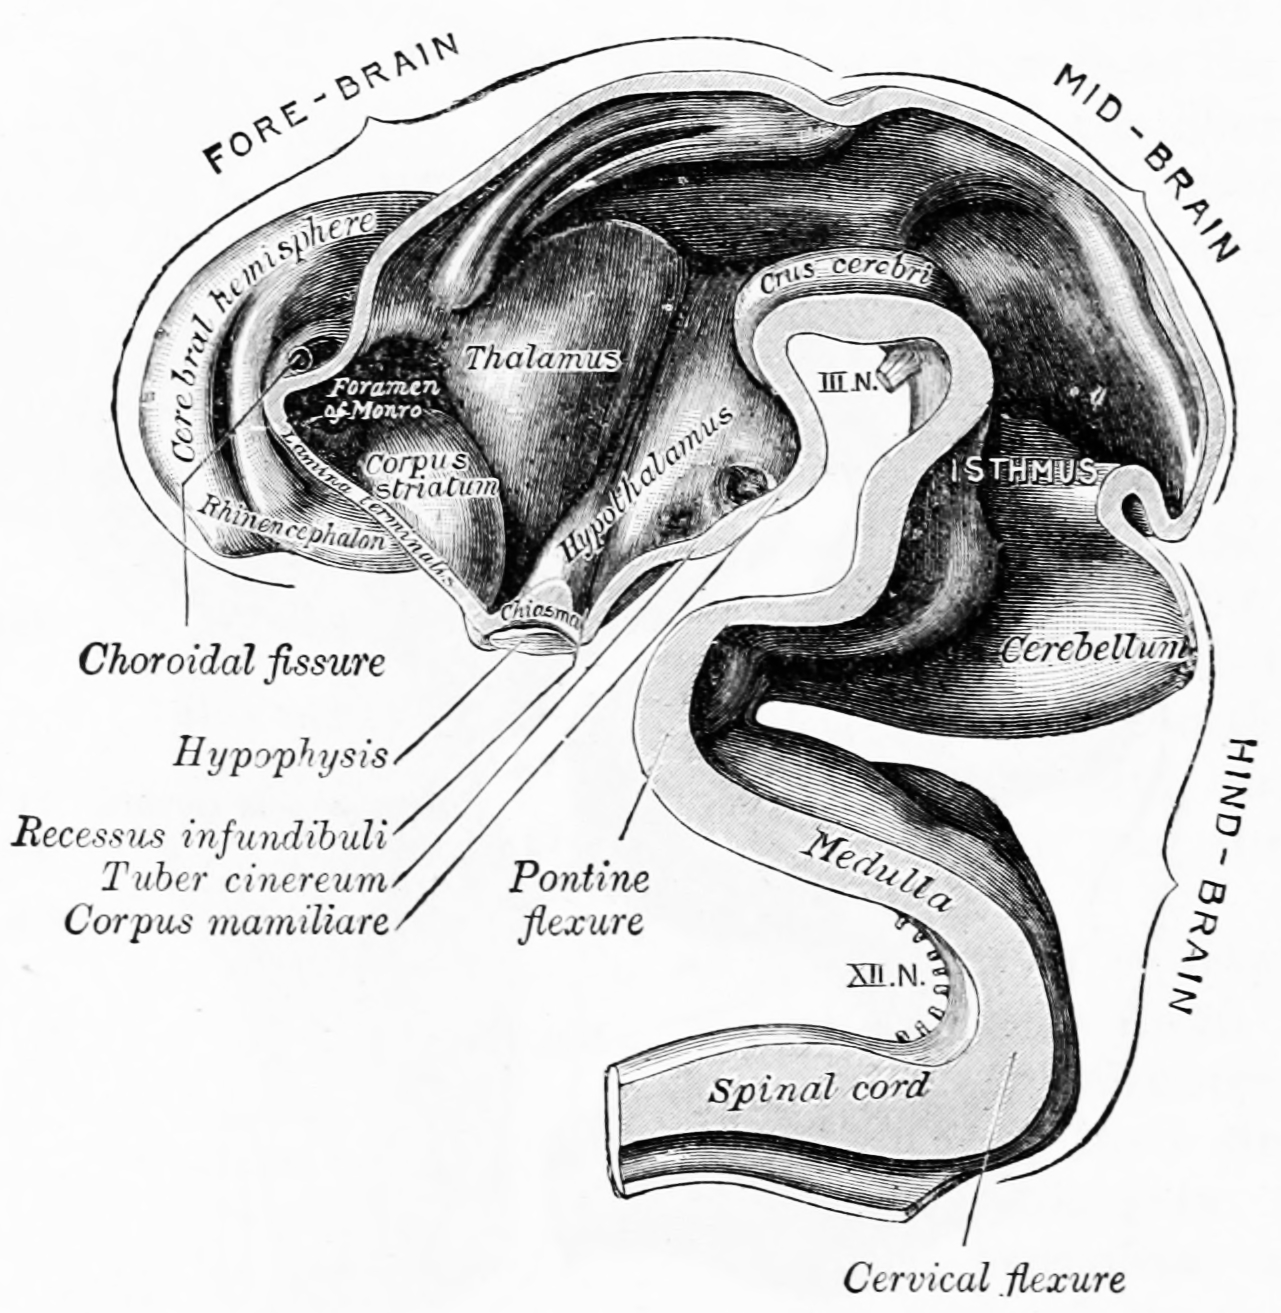
\includegraphics[width=0.7\linewidth]{./figures/development/GrayAnat1918p742} 

}

\caption{Interior of brain of human embryo of five weeks. From \href{https://archive.org/details/anatomyofhumanbo1918gray/page/n6/mode/2up}{Gray Henry, Anatomy of the Human Body. 20\textsuperscript{th} Edition, Lea \& Febiger, Philadelphia \& New York, 1918}}\label{fig:fiveinterior}
\end{figure}

The diencephalon, mesencephalon and rhombencephalon constitute the brain stem of the embryo. It continues to flex at the mesencephalon. The rhombencephalon folds posteriorly, which causes its alar plate to flare and form the fourth ventricle of the brain. The pons and the cerebellum form in the upper part of the rhombencephalon, whilst the medulla oblongata forms in the lower part.



\begin{figure}

{\centering 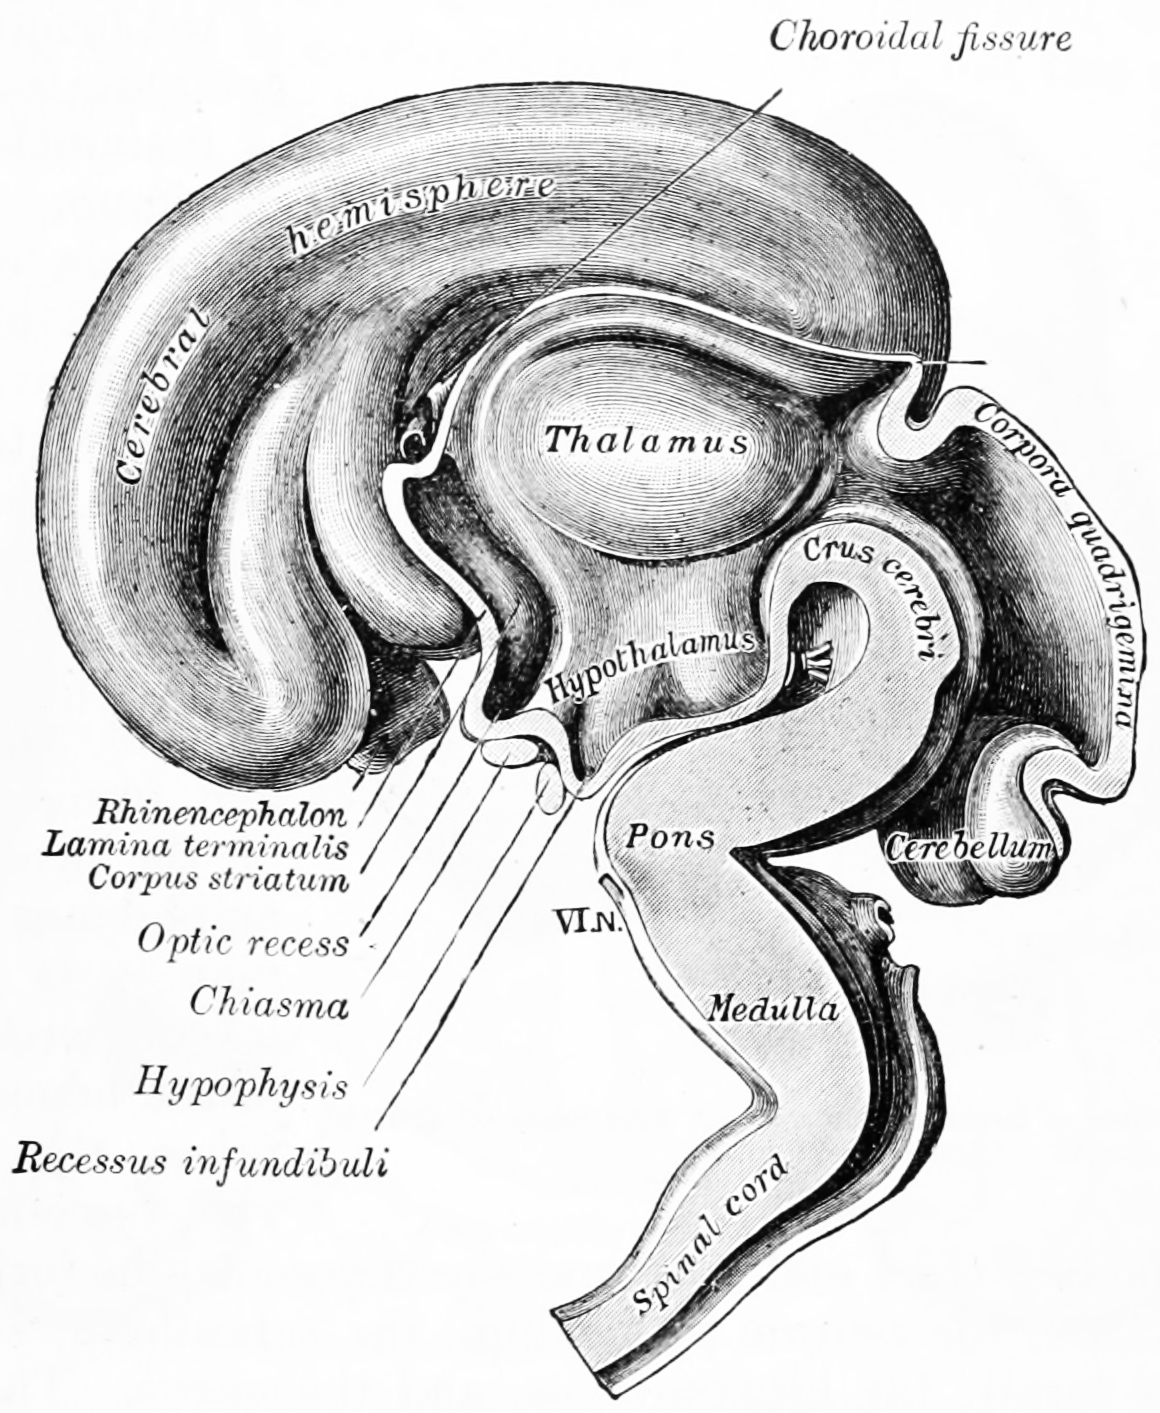
\includegraphics[width=0.7\linewidth]{./figures/development/GrayAnat1918p743} 

}

\caption{Interior of brain of human embryo of five weeks. From \href{https://archive.org/details/anatomyofhumanbo1918gray/page/n6/mode/2up}{Gray Henry, Anatomy of the Human Body. 20\textsuperscript{th} Edition, Lea \& Febiger, Philadelphia \& New York, 1918}}\label{fig:threemonths}
\end{figure}



\begin{figure}

{\centering 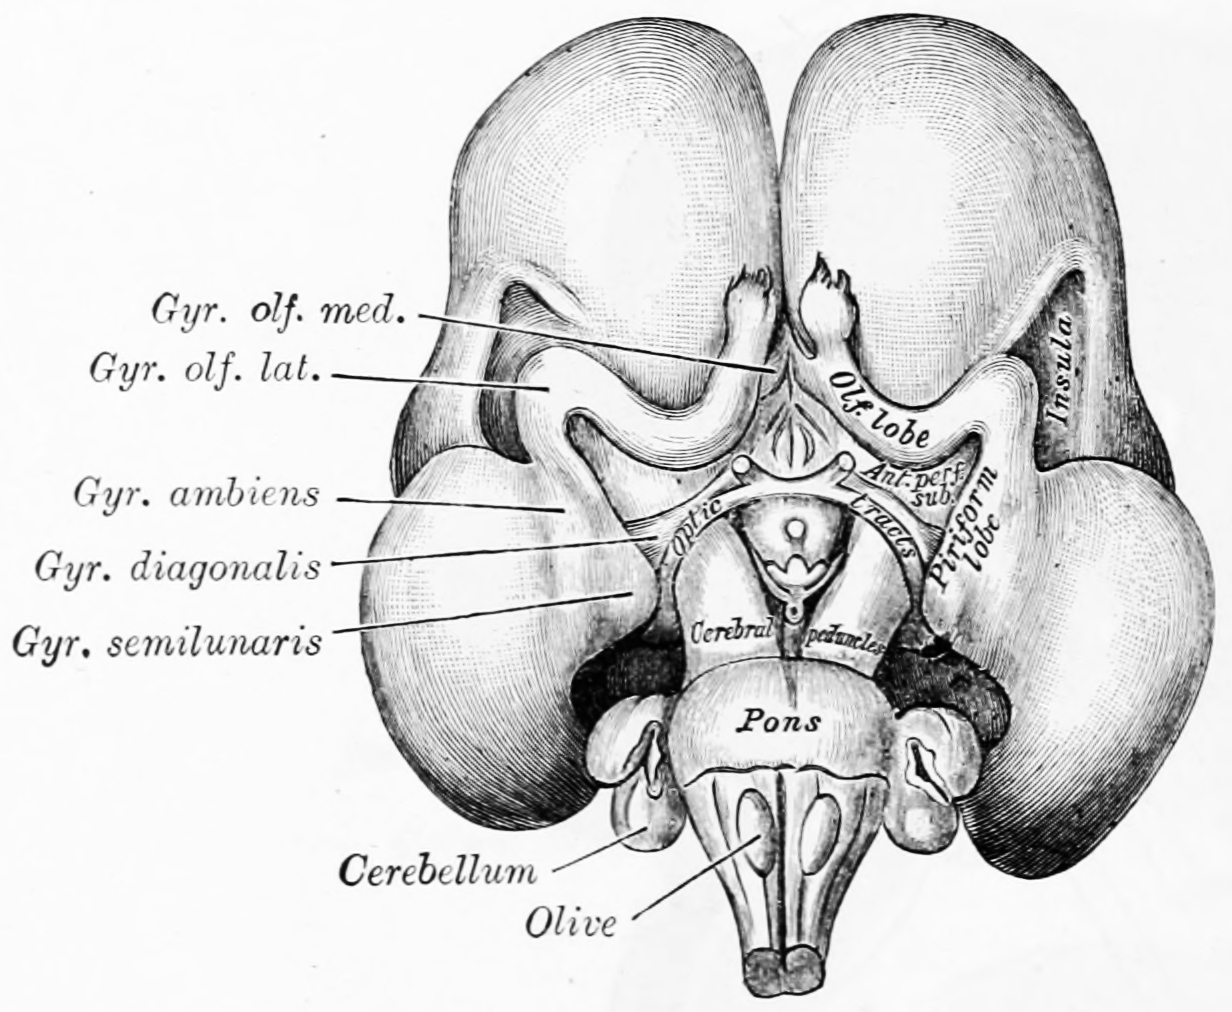
\includegraphics[width=0.7\linewidth]{./figures/development/GrayAnat1918p744} 

}

\caption{Inferior surface of brain of embryo at beginning of fourth month. From \href{https://archive.org/details/anatomyofhumanbo1918gray/page/n6/mode/2up}{Gray Henry, Anatomy of the Human Body. 20\textsuperscript{th} Edition, Lea \& Febiger, Philadelphia \& New York, 1918}}\label{fig:fourmonths}
\end{figure}



\begin{figure}

{\centering 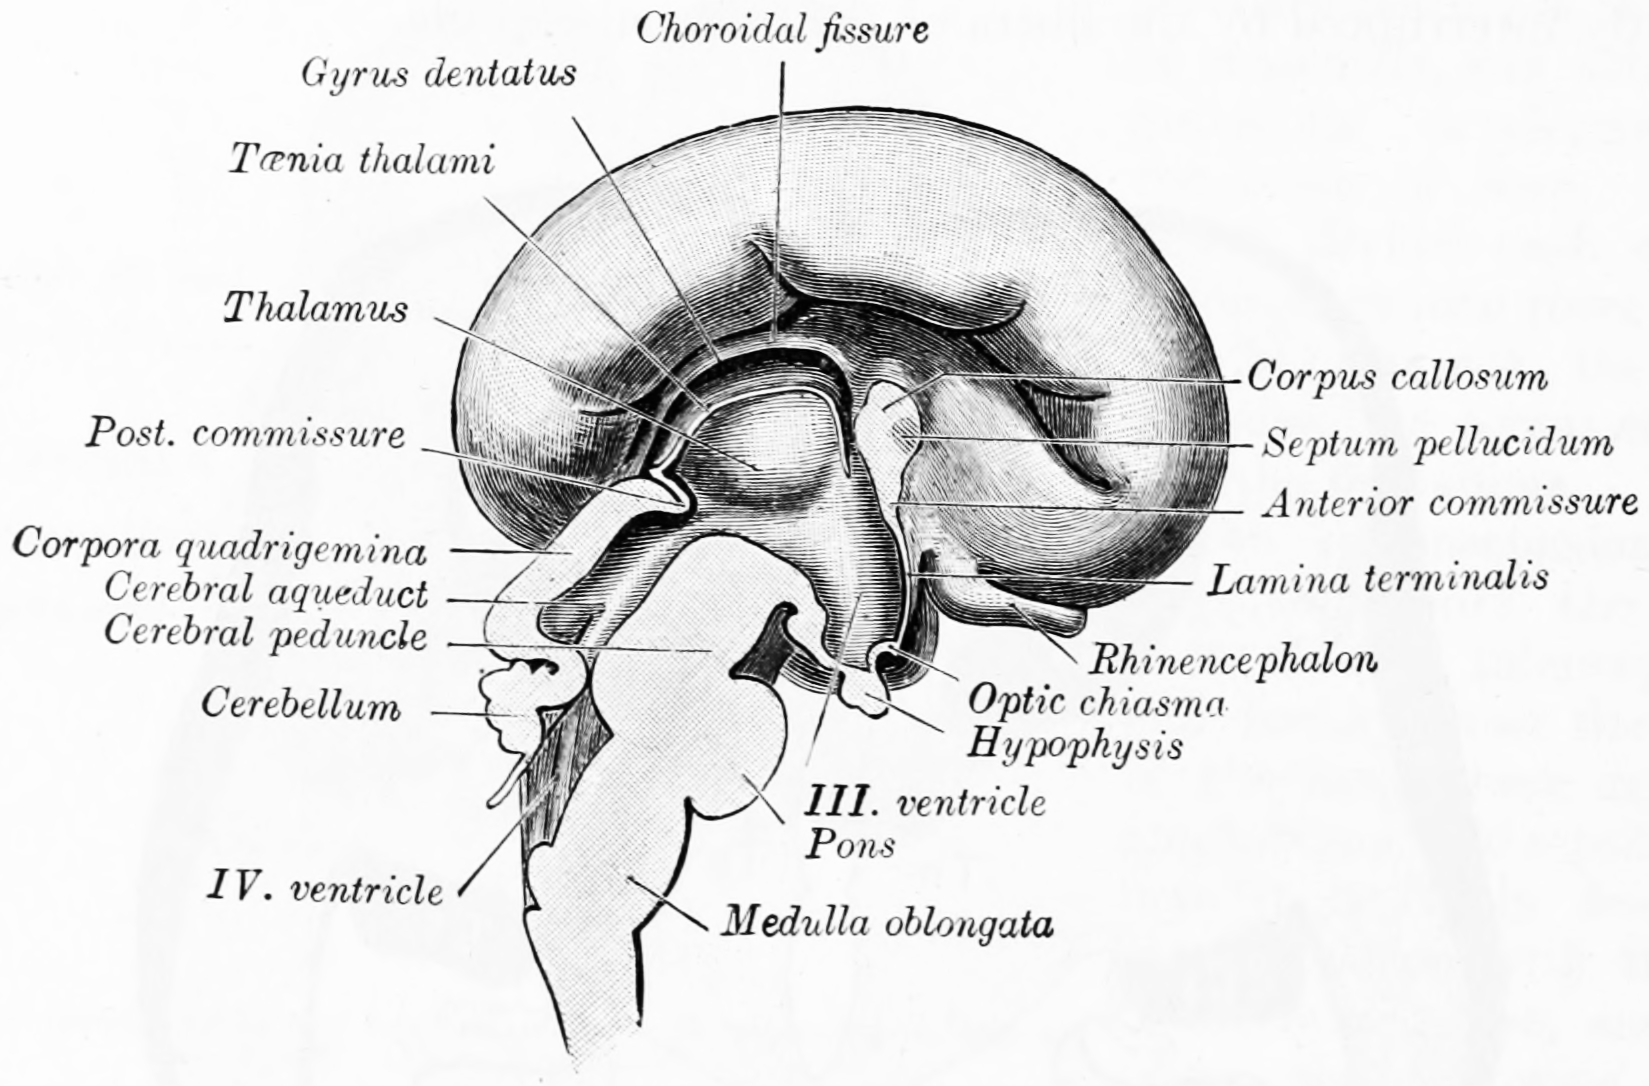
\includegraphics[width=0.7\linewidth]{./figures/development/GrayAnat1918p746} 

}

\caption{Median sagittal section of brain of human embryo of four months. From \href{https://archive.org/details/anatomyofhumanbo1918gray/page/n6/mode/2up}{Gray Henry, Anatomy of the Human Body. 20\textsuperscript{th} Edition, Lea \& Febiger, Philadelphia \& New York, 1918}}\label{fig:fourmonthsmedian}
\end{figure}

Some landmarks of neural development include the birth and differentiation of neurons from stem cell precursors, the migration of immature neurons from their birthplaces in the embryo to their final positions, outgrowth of axons and dendrites from neurons, guidance of the motile growth cone through the embryo towards postsynaptic partners, the generation of synapses between these axons and their postsynaptic partners, and finally the lifelong changes in synapses, which are thought to underlie learning and memory.



\begin{figure}

{\centering 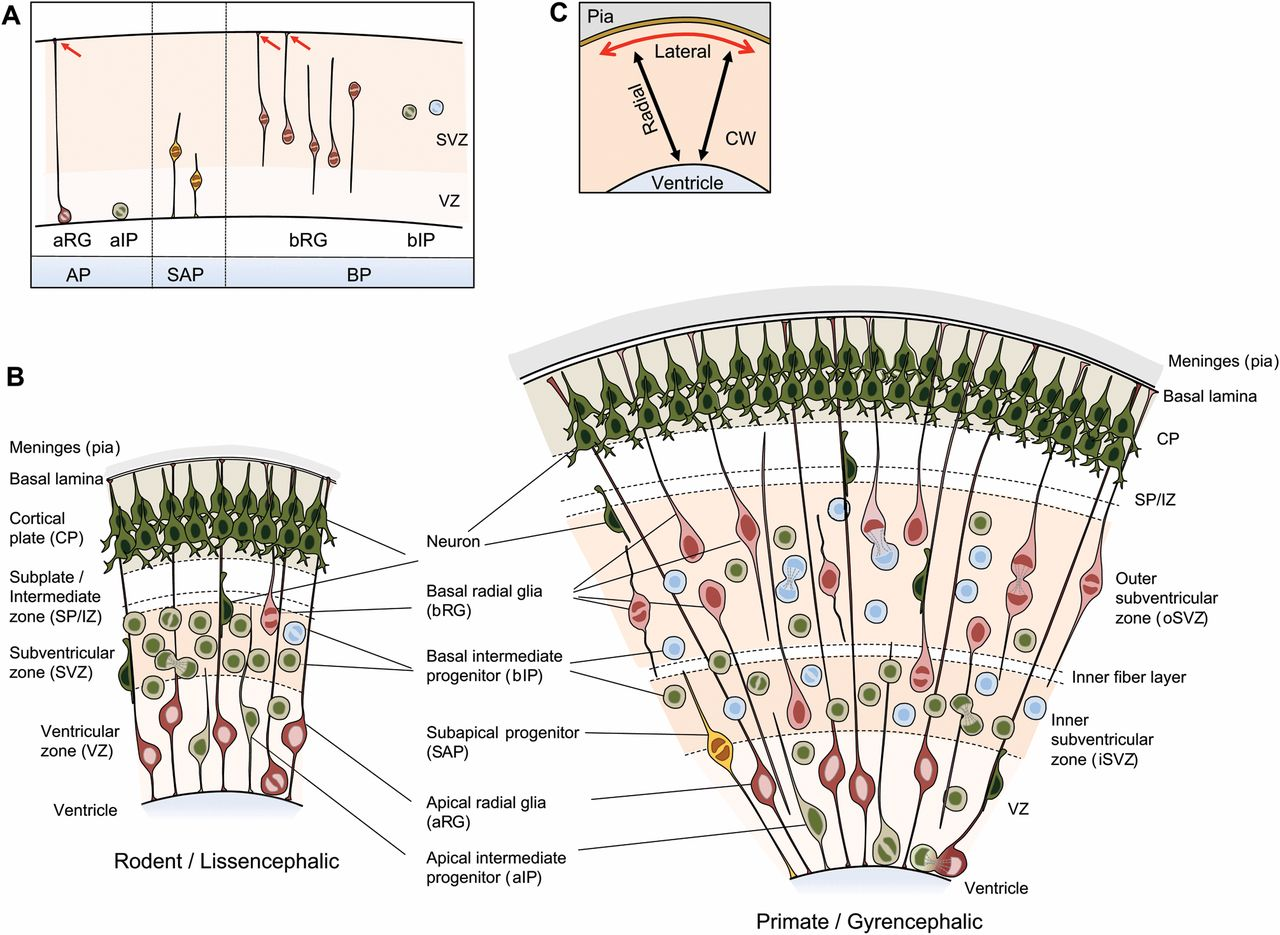
\includegraphics[width=0.7\linewidth]{./figures/development/neural_precursor} 

}

\caption{Neural precursor cell (NPC) types in the developing neocortex of representative lissencephalic and gyrencephalic species. (A) NPC types in the mammalian neocortex after the onset of neurogenesis, classified according to cell polarity, the presence of ventricular contact, and the location of mitosis. Red arrows indicate contact of the basal process with the basal lamina. Apical progenitors (APs), which include apical radial glia (aRG) and apical intermediate progenitors (aIPs), are defined by mitosis occurring at the ventricular surface and the presence of ventricular contact. Note that neuroepithelial cells (NECs), the primary APs that give rise to aRG and aIPs, are not depicted, as NECs prevail prior to the onset of neurogenesis. Subapical progenitors (SAPs) are defined by mitosis occurring at an abventricular location and the presence of ventricular contact. Basal progenitors (BPs), which comprise basal radial glia (bRG) and basal intermediate progenitors (bIPs), are defined by mitosis occurring at an abventricular location and the absence of ventricular contact. bRG subtypes (see Box 2 for more information) are also shown: proliferative bIP, blue; neurogenic bIP, green. (B) Coronal section of developing neocortex from a representative lissencephalic species, such as mouse or rat (left), and a representative gyrencephalic species, such as ferret or human (right), depicting the NPC types frequently observed in each of the germinal zones. (C) The major dimensions in which the developing neocortex is described: (1) radial (black arrows), i.e.~the ventricle-to-pia axis, corresponding to the apical-basal axis in terms of tissue polarity; and (2) lateral (red arrow), i.e.~the axis perpendicular to the radial axis. CW, cortical wall. From \href{https://dev.biologists.org/content/141/11/2182}{Marta Florio, Wieland B. Huttner(2014) Neural progenitors, neurogenesis and the evolution of the neocortex Development 2014 141: 2182-2194; doi: 10.1242/dev.090571}}\label{fig:neuralprecursor}
\end{figure}

Typically, these neurodevelopmental processes can be broadly divided into two classes: activity-independent mechanisms and activity-dependent mechanisms. Activity-independent mechanisms are generally believed to occur as hardwired processes determined by genetic programs played out within individual neurons. These include differentiation, migration and axon guidance to their initial target areas. These processes are thought of as being independent of neural activity and sensory experience. Once axons reach their target areas, activity-dependent mechanisms come into play. Although synapse formation is an activity-independent event, modification of synapses and synapse elimination requires neural activity.

Developmental neuroscience uses a variety of animal models including the mouse \emph{Mus musculus}, the fruit fly \emph{Drosophila melanogaster}, the zebrafish \emph{Danio rerio}, the frog Xenopus laevis, and the roundworm \emph{Caenorhabditis elegans}.

Myelination, formation of the lipid myelin bilayer around neuronal axons, is a process that is essential for normal brain function. The myelin sheath provides insulation for the nerve impulse when communicating between neural systems. Without it, the impulse would be disrupted and the signal would not reach its target, thus impairing normal functioning.

\hypertarget{patterning-of-the-nervous-system}{%
\section{Patterning Of The Nervous System}\label{patterning-of-the-nervous-system}}

In chordates, dorsal ectoderm forms all neural tissue and the nervous system. Patterning occurs due to specific environmental conditions - different concentrations of signaling molecules

The ventral half of the neural plate is controlled by the notochord, which acts as the `organiser'. The dorsal half is controlled by the ectoderm plate, which flanks either side of the neural plate.

Ectoderm follows a default pathway to become neural tissue. Evidence for this comes from single, cultured cells of ectoderm, which go on to form neural tissue. This is postulated to be because of a lack of BMPs, which are blocked by the organiser. The organiser may produce molecules such as follistatin, noggin and chordin that inhibit BMPs.

The ventral neural tube is patterned by sonic hedgehog (Shh) from the notochord, which acts as the inducing tissue. Notochord-derived Shh signals to the floor plate, and induces Shh expression in the floor plate. Floor plate-derived Shh subsequently signals to other cells in the neural tube, and is essential for proper specification of ventral neuron progenitor domains. Loss of Shh from the notochord and/or floor plate prevents proper specification of these progenitor domains. Shh binds Patched1, relieving Patched-mediated inhibition of Smoothened, leading to activation of the Gli family of transcription factors (GLI1, GLI2, and GLI3).

In this context Shh acts as a morphogen - it induces cell differentiation dependent on its concentration. At low concentrations it forms ventral interneurons, at higher concentrations it induces motor neuron development, and at highest concentrations it induces floor plate differentiation. Failure of Shh-modulated differentiation causes holoprosencephaly, a disorder in which the prosencephalon (the forebrain of the embryo) fails to develop into two hemispheres.

The dorsal neural tube is patterned by BMPs from the epidermal ectoderm flanking the neural plate. These induce sensory interneurons by activating Sr/Thr kinases and altering SMAD transcription factor levels.

Signals that control anteroposterior neural development include FGF and retinoic acid, which act in the hindbrain and spinal cord. The hindbrain, for example, is patterned by Hox genes, which are expressed in overlapping domains along the anteroposterior axis under the control of retinoic acid. The 3′ (3 prime end) genes in the Hox cluster are induced by retinoic acid in the hindbrain, whereas the 5′ (5 prime end) Hox genes are not induced by retinoic acid and are expressed more posteriorly in the spinal cord. Hoxb-1 is expressed in rhombomere 4 and gives rise to the facial nerve. Without this Hoxb-1 expression, a nerve similar to the trigeminal nerve arises.

\hypertarget{neurogenesis}{%
\section{Neurogenesis}\label{neurogenesis}}

Neurogenesis is the process by which neurons are generated from neural stem cells and progenitor cells. Neurons are `post-mitotic', meaning that they will never divide again for the lifetime of the organism.

Epigenetic modifications play a key role in regulating gene expression in differentiating neural stem cells and are critical for cell fate determination in the developing and adult mammalian brain. Epigenetic modifications include DNA cytosine methylation to form 5-methylcytosine and 5-methylcytosine demethylation. DNA cytosine methylation is catalyzed by DNA methyltransferases (DNMTs). Methylcytosine demethylation is catalyzed in several sequential steps by TET (\textbf{T}en-\textbf{e}leven \textbf{t}ranslocation methylcytosine dioxygenase) enzymes that carry out oxidative reactions (e.g.~5-methylcytosine to 5-hydroxymethylcytosine) and enzymes of the DNA base excision repair (BER) pathway.

\hypertarget{neuronal-migration}{%
\section{Neuronal Migration}\label{neuronal-migration}}

Neuronal precursor cells proliferate in the ventricular zone of the developing neocortex, where the principal neural stem cell is the radial glial cell. The first postmitotic cells must leave the stem cell niche and migrate outward to form the preplate, which is destined to become Cajal-Retzius cells and subplate neurons. These cells do so by somal translocation. Neurons migrating with this mode of locomotion are bipolar and attach the leading edge of the process to the pia. The soma is then transported to the pial surface by nucleokinesis, a process by which a microtubule ``cage'' around the nucleus elongates and contracts in association with the centrosome to guide the nucleus to its final destination. Radial glial cells, whose fibers serve as a scaffolding for migrating cells and a means of radial communication mediated by calcium dynamic activity, act as the main excitatory neuronal stem cell of the cerebral cortex or translocate to the cortical plate and differentiate either into astrocytes or neurons. Somal translocation can occur at any time during development.

Subsequent waves of neurons split the preplate by migrating along radial glial fibres to form the cortical plate. Each wave of migrating cells travel past their predecessors forming layers in an inside-out manner, meaning that the youngest neurons are the closest to the surface.

Most interneurons migrate tangentially through multiple modes of migration to reach their appropriate location in the cortex. An example of tangential migration is the movement of interneurons from the ganglionic eminence to the cerebral cortex. One example of ongoing tangential migration in a mature organism, observed in some animals, is the rostral migratory stream connecting subventricular zone and olfactory bulb.

Many neurons migrating along the anterior-posterior axis of the body use existing axon tracts to migrate along; this is called axophilic migration. An example of this mode of migration is in GnRH-expressing neurons, which make a long journey from their birthplace in the nose, through the forebrain, and into the hypothalamus. Many of the mechanisms of this migration have been worked out, starting with the extracellular guidance cues that trigger intracellular signaling. These intracellular signals, such as calcium signaling, lead to actin and microtubule cytoskeletal dynamics, which produce cellular forces that interact with the extracellular environment through cell adhesion proteins to cause the movement of these cells.

\hypertarget{neurotrophic-factors}{%
\section{Neurotrophic Factors}\label{neurotrophic-factors}}

The survival of neurons is regulated by survival factors, called trophic factors. The neurotrophic hypothesis was formulated by \href{https://en.wikipedia.org/wiki/Viktor_Hamburger}{Viktor Hamburger} and \href{https://en.wikipedia.org/wiki/Rita_Levi-Montalcini}{Rita Levi Montalcini} based on studies of the developing nervous system. Victor Hamburger discovered that implanting an extra limb in the developing chick led to an increase in the number of spinal motor neurons. Initially he thought that the extra limb was inducing proliferation of motor neurons, but he and his colleagues later showed that there was a great deal of motor neuron death during normal development, and the extra limb prevented this cell death. According to the neurotrophic hypothesis, growing axons compete for limiting amounts of target-derived trophic factors and axons that fail to receive sufficient trophic support die by apoptosis. It is now clear that factors produced by a number of sources contribute to neuronal survival.

\begin{itemize}
\tightlist
\item
  Nerve Growth Factor (NGF): Rita Levi Montalcini and \href{https://en.wikipedia.org/wiki/Stanley_Cohen_(biochemist)}{Stanley Cohen} purified the first trophic factor, Nerve Growth Factor, for which they received the Nobel Prize. There are three NGF-related trophic factors: BDNF, NT3, and NT4, which regulate survival of various neuronal populations. The Trk proteins act as receptors for NGF and related factors. Trk is a receptor tyrosine kinase. Trk dimerization and phosphorylation leads to activation of various intracellular signaling pathways including the MAP kinase, Akt, and PKC pathways.
\item
  CNTF: Ciliary neurotrophic factor is another protein that acts as a survival factor for motor neurons. CNTF acts via a receptor complex that includes CNTFRα, GP130, and LIFRβ. Activation of the receptor leads to phosphorylation and recruitment of the JAK kinase, which in turn phosphorylates LIFRβ. LIFRβ acts as a docking site for the STAT transcription factors. JAK kinase phosphorylates STAT proteins, which dissociate from the receptor and translocate to the nucleus to regulate gene expression.
\item
  GDNF: Glial derived neurotrophic factor is a member of the TGFb family of proteins, and is a potent trophic factor for striatal neurons. The functional receptor is a heterodimer, composed of type 1 and type 2 receptors. Activation of the type 1 receptor leads to phosphorylation of Smad proteins, which translocate to the nucleus to activate gene expression.
\end{itemize}

\hypertarget{activity-dependent-mechanisms-in-the-assembly-of-neural-circuits}{%
\section{Activity Dependent Mechanisms In The Assembly Of Neural Circuits}\label{activity-dependent-mechanisms-in-the-assembly-of-neural-circuits}}

The processes of neuronal migration, differentiation and axon guidance are generally believed to be activity-independent mechanisms and rely on hard-wired genetic programs in the neurons themselves. Research findings however have implicated a role for activity-dependent mechanisms in mediating some aspects of these processes such as the rate of neuronal migration, aspects of neuronal differentiation and axon pathfinding. Activity-dependent mechanisms influence neural circuit development and are crucial for laying out early connectivity maps and the continued refinement of synapses which occurs during development. There are two distinct types of neural activity we observe in developing circuits -early spontaneous activity and sensory-evoked activity. Spontaneous activity occurs early during neural circuit development even when sensory input is absent and is observed in many systems such as the developing visual system, auditory system, motor system, hippocampus, cerebellum and neocortex.

Experimental techniques such as direct electrophysiological recording, fluorescence imaging using calcium indicators and optogenetic techniques have shed light on the nature and function of these early bursts of activity. They have distinct spatial and temporal patterns during development and their ablation during development has been known to result in deficits in network refinement in the visual system. In the immature retina, waves of spontaneous action potentials arise from the retinal ganglion cells and sweep across the retinal surface in the first few postnatal weeks. These waves are mediated by neurotransmitter acetylcholine in the initial phase and later on by glutamate. They are thought to instruct the formation of two sensory maps- the retinotopic map and eye-specific segregation. Retinotopic map refinement occurs in downstream visual targets in the brain-the superior colliculus (SC) and dorsal lateral geniculate nucleus (LGN). Pharmacological disruption and mouse models lacking the β2 subunit of the nicotinic acetylcholine receptor has shown that the lack of spontaneous activity leads to marked defects in retinotopy and eye-specific segregation.

In the developing auditory system, developing cochlea generate bursts of activity which spreads across the inner hair cells and spiral ganglion neurons which relay auditory information to the brain. ATP release from supporting cells triggers action potentials in inner hair cells. In the auditory system, spontaneous activity is thought to be involved in tonotopic map formation by segregating cochlear neuron axons tuned to high and low frequencies. In the motor system, periodic bursts of spontaneous activity are driven by excitatory GABA and glutamate during the early stages and by acetylcholine and glutamate at later stages. In the cortex, early waves of activity have been observed in the cerebellum and cortical slices. Once sensory stimulus becomes available, final fine-tuning of sensory-coding maps and circuit refinement begins to rely more and more on sensory-evoked activity as demonstrated by classic experiments about the effects of sensory deprivation during critical periods.

\hypertarget{neurons-and-glial-cells}{%
\chapter{Neurons And Glial Cells}\label{neurons-and-glial-cells}}

\hypertarget{neurons}{%
\section{Neurons}\label{neurons}}

The neuron doctrine is the now fundamental idea that neurons are the basic structural and functional units of the nervous system. The theory was put forward by Santiago Ramón y Cajal in the late 19th century. It held that neurons are discrete cells (not connected in a meshwork), acting as metabolically distinct units.

Later discoveries yielded refinements to the doctrine. For example, glial cells, which are not considered neurons, play an essential role in information processing. Also, electrical synapses are more common than previously thought, comprising direct, cytoplasmic connections between neurons. In fact, neurons can form even tighter couplings: the squid giant axon arises from the fusion of multiple axons.

Ramón y Cajal also postulated the Law of Dynamic Polarization, which states that a neuron receives signals at its dendrites and cell body and transmits them, as action potentials, along the axon in one direction: away from the cell body. The Law of Dynamic Polarization has important exceptions; dendrites can serve as synaptic output sites of neurons and axons can receive synaptic inputs.

The number of neurons in the brain varies dramatically from species to species. In a human, there are an estimated 10--20 billion neurons in the cerebral cortex and 55--70 billion neurons in the cerebellum. By contrast, the nematode worm \emph{Caenorhabditis elegans} has just 302 neurons, making it an ideal model organism as scientists have been able to map all of its neurons. The fruit fly \emph{Drosophila melanogaster}, a common subject in biological experiments, has around 100,000 neurons and exhibits many complex behaviors. Many properties of neurons, from the type of neurotransmitters used to ion channel composition, are maintained across species, allowing scientists to study processes occurring in more complex organisms in much simpler experimental systems.

A neuron, neurone (old British spelling) or nerve cell, is an electrically excitable cell that communicates with other cells via specialized connections called synapses. It is the main component of nervous tissue. All animals except sponges and placozoans have neurons, but other multicellular organisms such as plants do not.

Neurons are typically classified into three types based on their function. Sensory neurons respond to stimuli such as touch, sound, or light that affect the cells of the sensory organs, and they send signals to the spinal cord or brain. Motor neurons receive signals from the brain and spinal cord to control everything from muscle contractions to glandular output. Interneurons connect neurons to other neurons within the same region of the brain or spinal cord. A group of connected neurons is called a neural circuit.

A typical neuron consists of a cell body (soma), dendrites, and a single axon. The soma is usually compact. The axon and dendrites are filaments that extrude from it. Dendrites typically branch profusely and extend a few hundred micrometers from the soma. The axon leaves the soma at a swelling called the axon hillock, and travels for as far as 1 meter in humans or more in other species. It branches but usually maintains a constant diameter. At the farthest tip of the axon's branches are axon terminals, where the neuron can transmit a signal across the synapse to another cell. Neurons may lack dendrites or have no axon. The term neurite is used to describe either a dendrite or an axon, particularly when the cell is undifferentiated.

Most neurons receive signals via the dendrites and soma and send out signals down the axon. At the majority of synapses, signals cross from the axon of one neuron to a dendrite of another. However, synapses can connect an axon to another axon or a dendrite to another dendrite.

The signaling process is partly electrical and partly chemical. Neurons are electrically excitable, due to maintenance of voltage gradients across their membranes. If the voltage changes by a large enough amount over a short interval, the neuron generates an all-or-nothing electrochemical pulse called an action potential. This potential travels rapidly along the axon, and activates synaptic connections as it reaches them. Synaptic signals may be excitatory or inhibitory, increasing or reducing the net voltage that reaches the soma.

In most cases, neurons are generated by neural stem cells during brain development and childhood. Neurogenesis largely ceases during adulthood in most areas of the brain. However, strong evidence supports generation of substantial numbers of new neurons in the hippocampus and olfactory bulb.

Neurons are highly specialized for the processing and transmission of cellular signals. Given their diversity of functions performed in different parts of the nervous system, there is a wide variety in their shape, size, and electrochemical properties. For instance, the soma of a neuron can vary from 4 to 100 micrometers in diameter.

The soma is the body of the neuron. As it contains the nucleus, most protein synthesis occurs here. The nucleus can range from 3 to 18 micrometers in diameter.
The dendrites of a neuron are cellular extensions with many branches. This overall shape and structure is referred to metaphorically as a dendritic tree. This is where the majority of input to the neuron occurs via the dendritic spine.

The axon is a finer, cable-like projection that can extend tens, hundreds, or even tens of thousands of times the diameter of the soma in length. The axon primarily carries nerve signals away from the soma, and carries some types of information back to it. Many neurons have only one axon, but this axon may---and usually will---undergo extensive branching, enabling communication with many target cells. The part of the axon where it emerges from the soma is called the axon hillock. Besides being an anatomical structure, the axon hillock also has the greatest density of voltage-dependent sodium channels. This makes it the most easily excited part of the neuron and the spike initiation zone for the axon. In electrophysiological terms, it has the most negative threshold potential. While the axon and axon hillock are generally involved in information outflow, this region can also receive input from other neurons.

The axon terminal is found at the end of the axon farthest from the soma and contains synapses. Synaptic boutons are specialized structures where neurotransmitter chemicals are released to communicate with target neurons. In addition to synaptic boutons at the axon terminal, a neuron may have en passant boutons, which are located along the length of the axon.

The accepted view of the neuron attributes dedicated functions to its various anatomical components; however, dendrites and axons often act in ways contrary to their so-called main function.

Axons and dendrites in the central nervous system are typically only about one micrometer thick, while some in the peripheral nervous system are much thicker. The soma is usually about 10--25 micrometers in diameter and often is not much larger than the cell nucleus it contains. The longest axon of a human motor neuron can be over a meter long, reaching from the base of the spine to the toes.

Sensory neurons can have axons that run from the toes to the posterior column of the spinal cord, over 1.5 meters in adults. Giraffes have single axons several meters in length running along the entire length of their necks. Much of what is known about axonal function comes from studying the squid giant axon, an ideal experimental preparation because of its relatively immense size (0.5--1 millimeters thick, several centimeters long).

Fully differentiated neurons are permanently postmitotic however, stem cells present in the adult brain may regenerate functional neurons throughout the life of an organism. Astrocytes are star-shaped glial cells. They have been observed to turn into neurons by virtue of their stem cell-like characteristic of pluripotency.

Like all animal cells, the cell body of every neuron is enclosed by a plasma membrane, a bilayer of lipid molecules with many types of protein structures embedded in it. A lipid bilayer is a powerful electrical insulator, but in neurons, many of the protein structures embedded in the membrane are electrically active. These include ion channels that permit electrically charged ions to flow across the membrane and ion pumps that transport ions from one side of the membrane to the other. Most ion channels are permeable only to specific types of ions. Some ion channels are voltage gated, meaning that they can be switched between open and closed states by altering the voltage difference across the membrane. Others are chemically gated, meaning that they can be switched between open and closed states by interactions with chemicals that diffuse through the extracellular fluid. The ions include sodium, potassium, chloride, and calcium. The interactions between ion channels and ion pumps produce a voltage difference across the membrane, typically a bit less than 1/10 of a volt at baseline. This voltage has two functions: first, it provides a power source for an assortment of voltage-dependent protein machinery that is embedded in the membrane; second, it provides a basis for electrical signal transmission between different parts of the membrane.

Numerous microscopic clumps called Nissl bodies (or Nissl substance) are seen when nerve cell bodies are stained with a basophilic (``base-loving'') dye. These structures consist of rough endoplasmic reticulum and associated ribosomal RNA. Named after German psychiatrist and neuropathologist \href{https://en.wikipedia.org/wiki/Franz_Nissl}{Franz Nissl} (1860--1919), they are involved in protein synthesis and their prominence can be explained by the fact that nerve cells are very metabolically active. Basophilic dyes such as aniline or (weakly) haematoxylin highlight negatively charged components, and so bind to the phosphate backbone of the ribosomal RNA.

The cell body of a neuron is supported by a complex mesh of structural proteins called neurofilaments, which together with neurotubules (neuronal microtubules) are assembled into larger neurofibrils. Some neurons also contain pigment granules, such as neuromelanin (a brownish-black pigment that is byproduct of synthesis of catecholamines), and lipofuscin (a yellowish-brown pigment), both of which accumulate with age. Other structural proteins that are important for neuronal function are actin and the tubulin of microtubules. Class III β-tubulin is found almost exclusively in neurons. Actin is predominately found at the tips of axons and dendrites during neuronal development. There the actin dynamics can be modulated via an interplay with microtubule.



\begin{figure}

{\centering 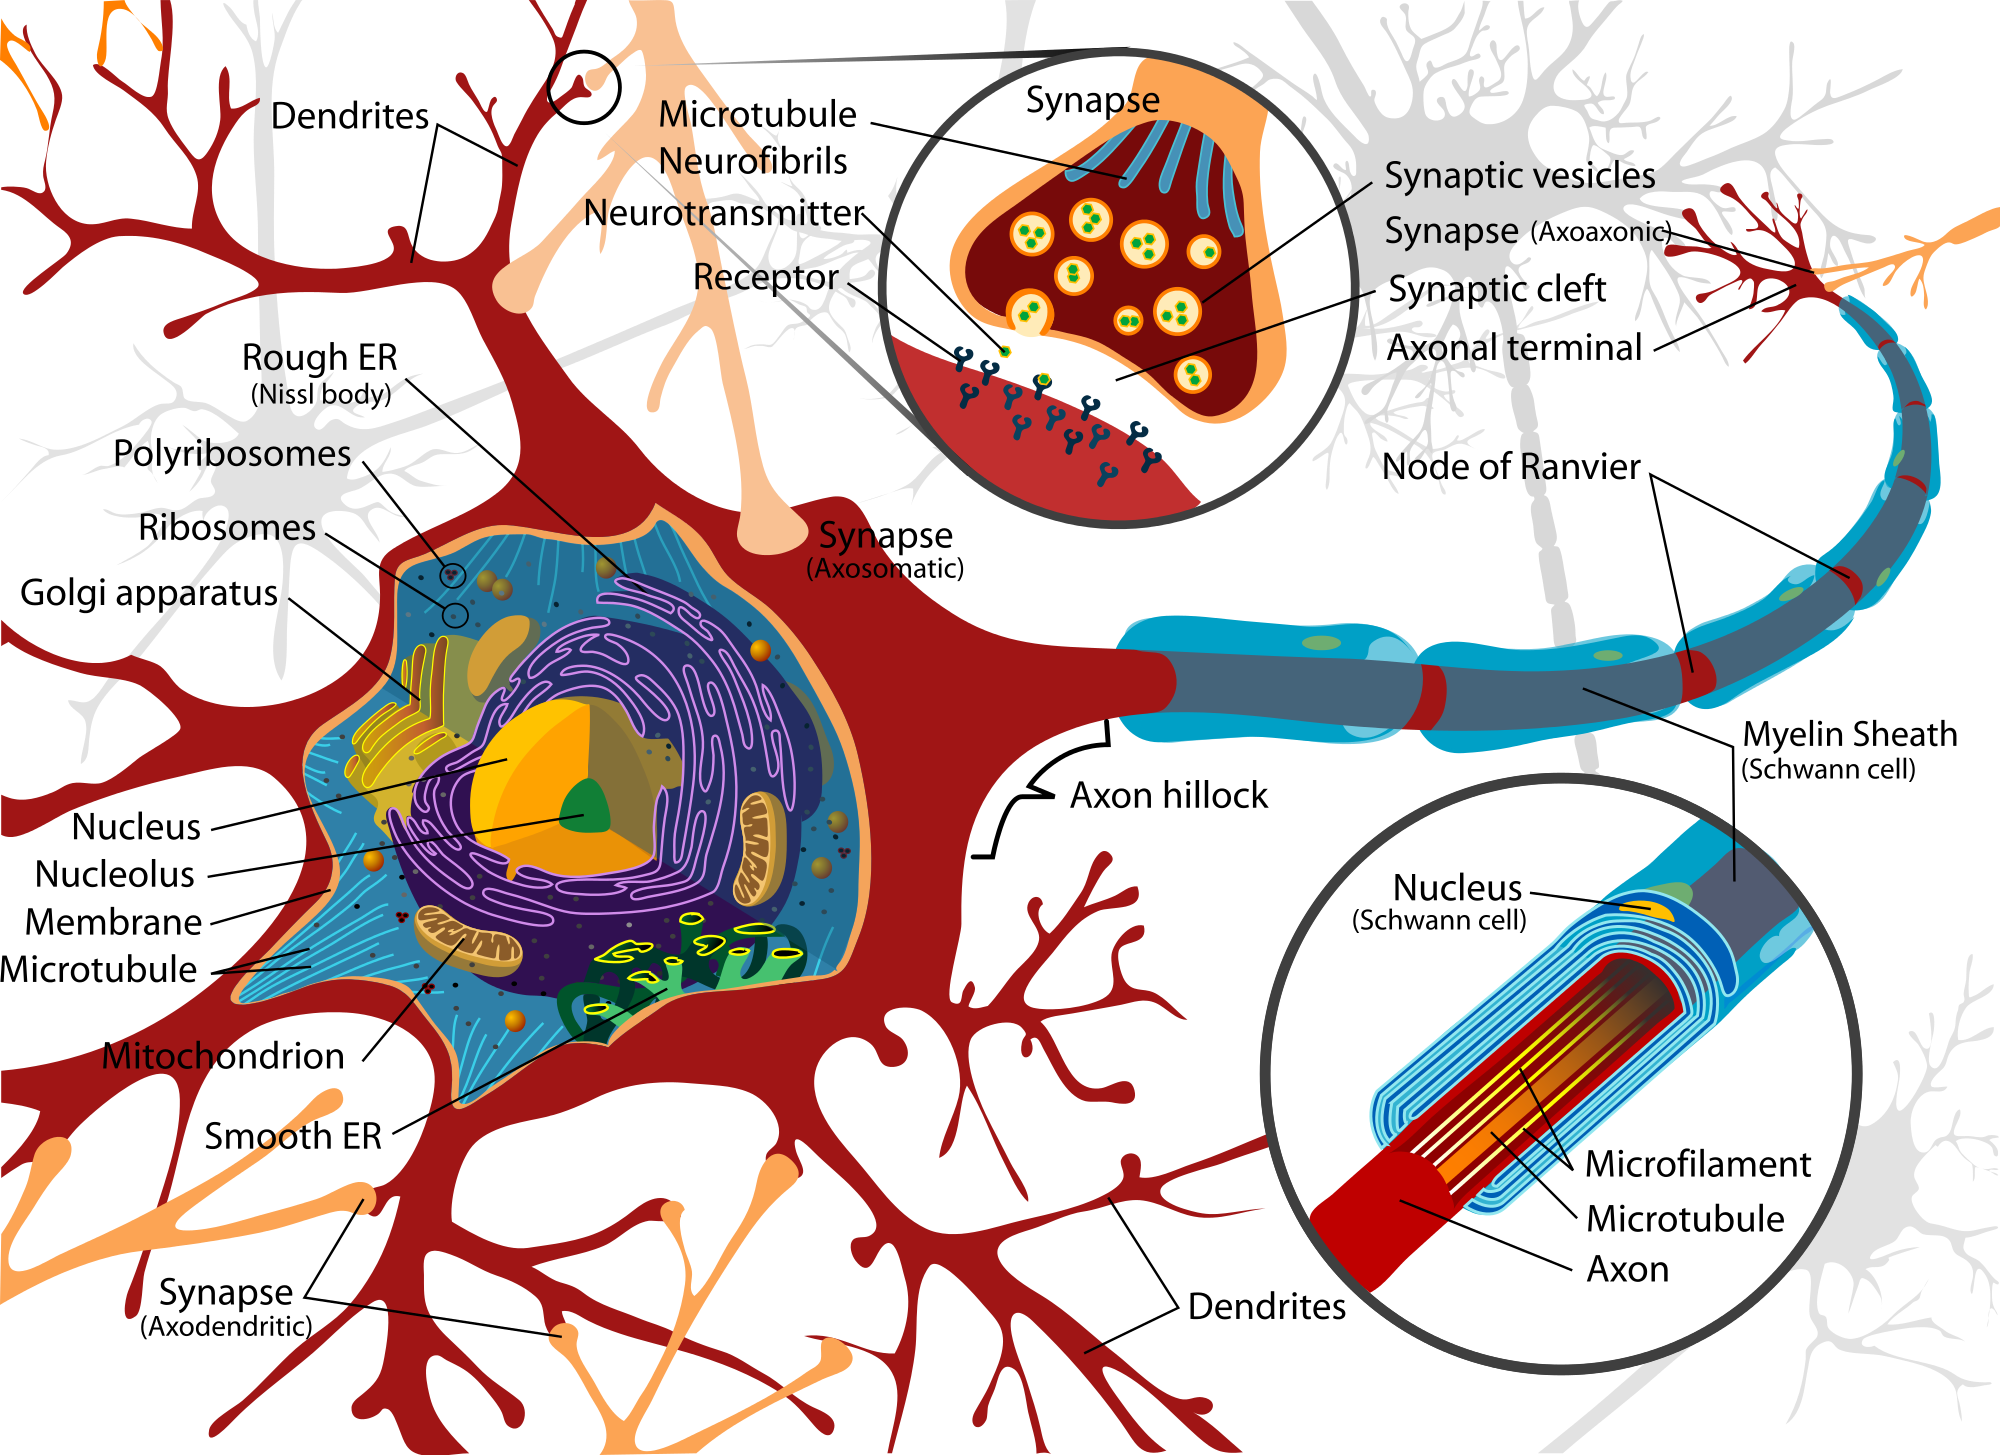
\includegraphics[width=0.7\linewidth]{./figures/cells/Complete_neuron_cell_diagram_en} 

}

\caption{\href{https://commons.wikimedia.org/wiki/File:Complete_neuron_cell_diagram_en.svg}{Diagram of a myelinated vertebrate motor neuron.}}\label{fig:motorneuron}
\end{figure}

There are different internal structural characteristics between axons and dendrites. Typical axons almost never contain ribosomes, except some in the initial segment. Dendrites contain granular endoplasmic reticulum or ribosomes, in diminishing amounts as the distance from the cell body increases.

Neurons vary in shape and size and can be classified by their morphology and function. The anatomist \href{https://en.wikipedia.org/wiki/Camillo_Golgi}{Camillo Golgi} grouped neurons into two types; type I with long axons used to move signals over long distances and type II with short axons, which can often be confused with dendrites. Type I cells can be further classified by the location of the soma. The basic morphology of type I neurons, represented by spinal motor neurons, consists of a cell body called the soma and a long thin axon covered by a myelin sheath.



\begin{figure}

{\centering 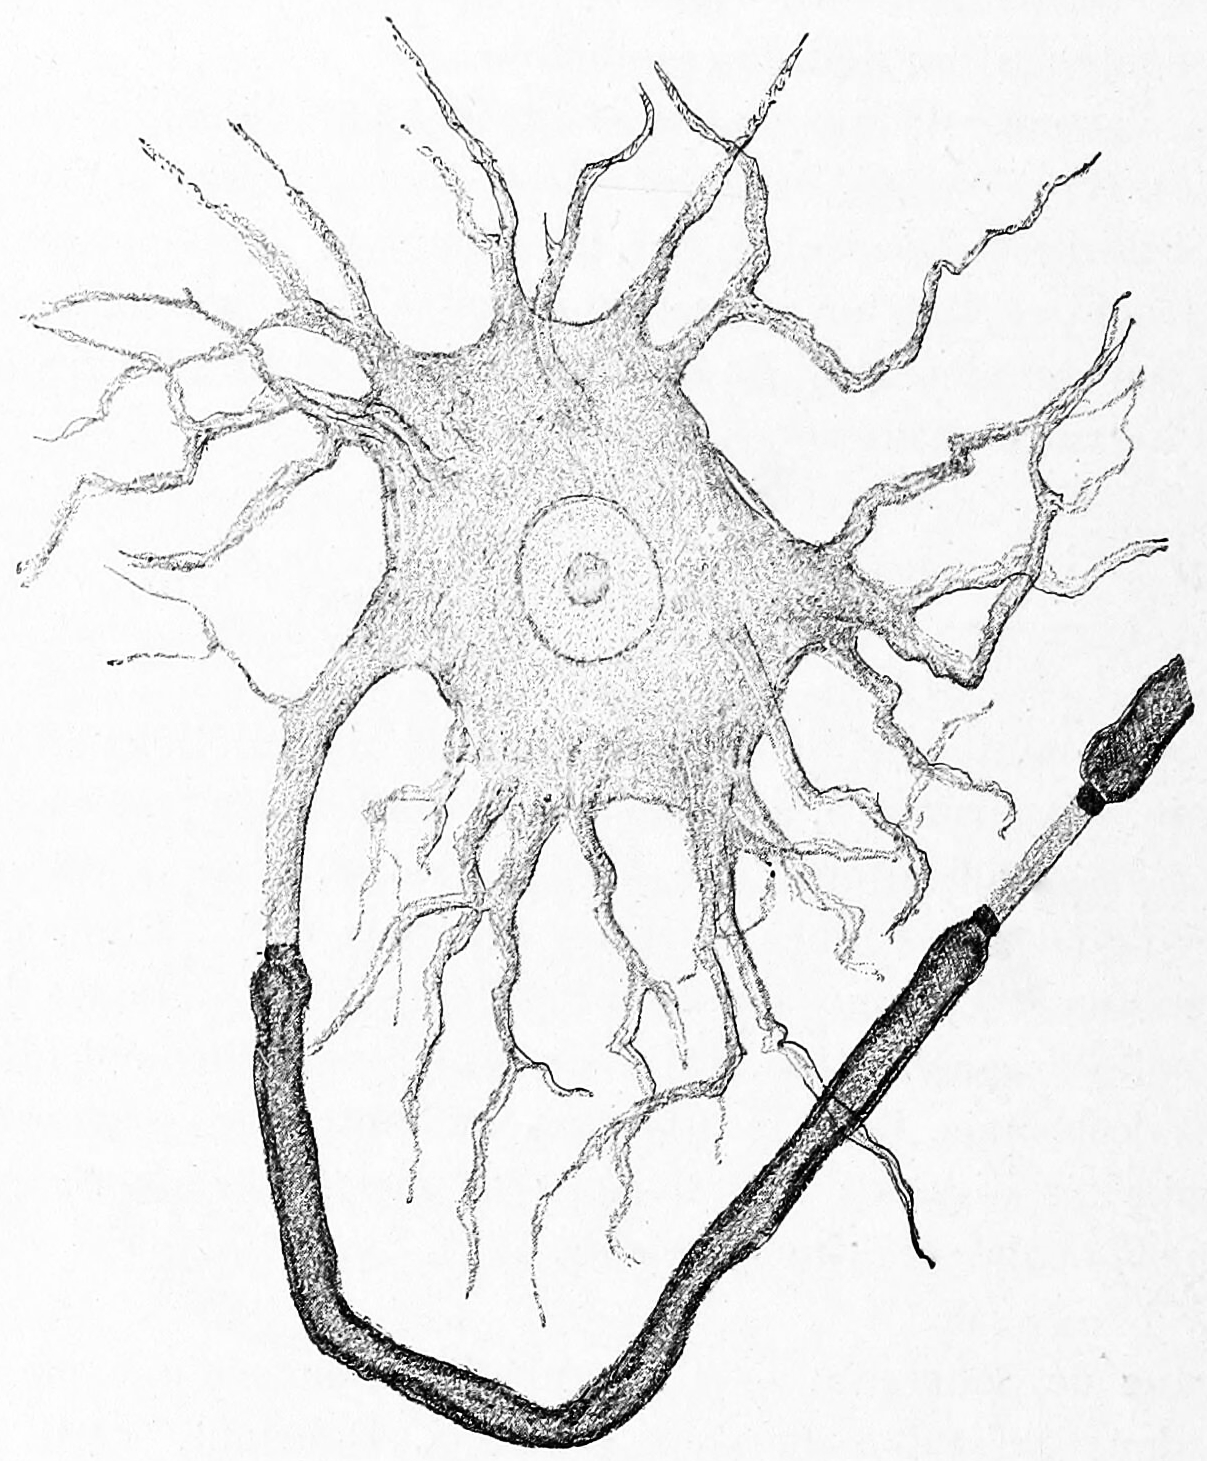
\includegraphics[width=0.7\linewidth]{./figures/cells/CajalMyelinAxon} 

}

\caption{A Golgi type I neuron from the electric lobe in the brain of the electric ray (\emph{Torpedo}). A single, thick axon emerges from the cell body unmyelinated (middle, left) but becomes surrounded by a think layer of myelin (dark grey). Multiple, thin dendrites emerge from the remainder of the cell body. \href{https://wellcomelibrary.org/item/b2129592x\#?c=0\&m=0\&s=0\&cv=14\&z=0\%2C-3.48\%2C1\%2C8.6591}{Histologie du système nerveux de l'homme \& des vertébrés, Tome Premier} (1909) by Santiago Ramón y Cajal translated from Spanish by Dr.~L. Azoulay.}\label{fig:axonmyelinated}
\end{figure}

The dendritic tree wraps around the cell body and receives signals from other neurons. The end of the axon has branching terminals (axon terminal) that release neurotransmitters into a gap called the synaptic cleft between the terminals and the dendrites of the next neuron.

Most neurons can be anatomically characterized as:

\begin{itemize}
\tightlist
\item
  Unipolar: single process
\item
  Bipolar: 1 axon and 1 dendrite
\item
  Multipolar: 1 axon and 2 or more dendrites
\item
  Golgi I: neurons with projecting axonal processes; examples are pyramidal cells, Purkinje cells, and anterior horn cells
\item
  Golgi II: neurons whose axonal process projects locally; the best example is the granule cell
\item
  Anaxonic: where the axon cannot be distinguished from the dendrite(s)
\item
  Pseudounipolar: 1 process which then serves as both an axon and a dendrite
\item
  Other
\end{itemize}



\begin{figure}

{\centering \includegraphics[width=0.7\linewidth]{./figures/cells/Cajal_neurons} 

}

\caption{Morpholoigcally distinct types of neurons after Cajal. A) Unipolar neurons; B) bipolar neurons; Golgi I neurons: C) a Purkinje cell; D) spinal motor neuron E) a pyramidal cell; F) Golgi II neuron. \href{https://wellcomelibrary.org/item/b2129592x\#?c=0\&m=0\&s=0\&cv=14\&z=0\%2C-3.48\%2C1\%2C8.6591}{Histologie du système nerveux de l'homme \& des vertébrés, Tome Premier} (1909) by Santiago Ramón y Cajal translated from Spanish by Dr.~L. Azoulay.}\label{fig:neurontypes}
\end{figure}

Some unique neuronal types can be identified according to their location in the nervous system and distinct shape. Some examples are:

\begin{itemize}
\tightlist
\item
  Basket cells, interneurons that form a dense plexus of terminals around the soma of target cells, found in the cortex and cerebellum
\item
  Betz cells, large motor neurons
\item
  Lugaro cells, interneurons of the cerebellum
\item
  Medium spiny neurons, most neurons in the corpus striatum
\item
  Purkinje cells, huge neurons in the cerebellum, a type of Golgi I multipolar neuron
\item
  Pyramidal cells, neurons with triangular soma, a type of Golgi I
\item
  Renshaw cells, neurons with both ends linked to alpha motor neurons
\item
  Unipolar brush cells, interneurons with unique dendrite ending in a brush-like tuft
\item
  Granule cells, a type of Golgi II neuron
\item
  Anterior horn cells, motoneurons located in the spinal cord
\item
  Spindle cells, interneurons that connect widely separated areas of the brain
\end{itemize}

Neurons can also be characterized based on various aspects of their function:

\begin{itemize}
\tightlist
\item
  Afferent neurons convey information from tissues and organs into the central nervous system and are also called sensory neurons.
\item
  Efferent neurons (motor neurons) transmit signals from the central nervous system to the effector cells.
\item
  Interneurons connect neurons within specific regions of the central nervous system.
  Afferent and efferent also refer generally to neurons that, respectively, bring information to or send information from the brain.
\end{itemize}

The axons of neurons in the human peripheral nervous system can be classified based on their physical features and signal conduction properties. Axons were known to have different thicknesses (from 0.1 to 20 µm) and these differences were thought to relate to the speed at which an action potential could travel along the axon -- its conductance velocity. Erlanger and Gasser proved this hypothesis, and identified several types of nerve fiber, establishing a relationship between the diameter of an axon and its nerve conduction velocity. They published their findings in 1941 giving the first classification of axons.

Axons are classified in two systems. The first one introduced by Erlanger and Gasser, grouped the fibers into three main groups using the letters A, B, and C. These groups, group A, group B, and group C include both the sensory fibers (afferents) and the motor fibres (efferents). The first group A, was subdivided into alpha, beta, gamma, and delta fibers --- Aα, Aβ, Aγ, and Aδ. The motor neurons of the different motor fibers, were the lower motor neurons -- alpha motor neuron, beta motor neuron, and gamma motor neuron having the Aα, Aβ, and Aγ nerve fibers respectively.

\begin{longtable}[t]{>{\raggedright\arraybackslash}p{5em}>{\raggedright\arraybackslash}p{5em}>{\raggedright\arraybackslash}p{5em}>{\raggedright\arraybackslash}p{5em}>{\raggedright\arraybackslash}p{5em}>{\raggedright\arraybackslash}p{10em}}
\caption{\label{tab:erlanger}Erlanger Gasser Classification of Lower Motor Neuron Fiber Types}\\
\toprule
Type & Erlanger-Gasser Classification & Diameter (µm) & Myelin & Conduction Velocity (m/s) & Associated Muscle Fibers\\
\midrule
\rowcolor{gray!6}  α & Aα & 13-20 & Yes & 80–120 & Extrafusal muscle fibers\\
β & Aβ &  &  &  & \\
\rowcolor{gray!6}  γ & Aγ & 5-8 & Yes & 4–24 & Intrafusal muscle fibers\\
\bottomrule
\end{longtable}

Later findings by other researchers identified two groups of Aα fibers that were sensory fibers. These were then introduced into a system that only included sensory fibers (though some of these were mixed nerves and were also motor fibers). This system refers to the sensory groups as types and uses Roman numerals: Type Ia, Type Ib, Type II, Type III, and Type IV.

\begin{longtable}[t]{>{\raggedright\arraybackslash}p{5em}>{\raggedright\arraybackslash}p{5em}>{\raggedright\arraybackslash}p{5em}>{\raggedright\arraybackslash}p{5em}>{\raggedright\arraybackslash}p{5em}>{\raggedright\arraybackslash}p{5em}>{\raggedright\arraybackslash}p{5em}}
\caption{\label{tab:sensory}Erlanger Gasser Classification of Sensory Fiber Types}\\
\toprule
Type & Erlanger-Gasser Classification & Diameter (µm) & Myelin & Conduction Velocity (m/s) & Associated Sensory Receptors & Function\\
\midrule
\rowcolor{gray!6}  Ia & Aα & 13-20 & Yes & 80–120 & Primary receptors of muscle spindle (annulospiral ending) & Proprioceptors\\
Ib & Aα & 13-20 & Yes & 80–120 & Golgi tendon organ & Proprioceptors\\
\rowcolor{gray!6}  II & Aβ & 6-12 & Yes & 33–75 & Secondary receptors of muscle spindle (flower-spray ending). All cutaneous mechanoreceptors & Proprioceptors; mechanoceptors\\
III & Aδ & 1-5 & Thin & 3–30 & Free nerve endings of touch and pressure; nociceptors of lateral spinothalamic tract; cold thermoreceptors & Mechanoceptors; nociceptors and thermoreceptors\\
\rowcolor{gray!6}  IV & C & 0.2-1.5 & No & 0.5-2.0 & Nociceptors of anterior spinothalamic tract; warmth receptors & Nociceptors and thermoreceptors\\
\bottomrule
\end{longtable}

Neurons have intrinsic electroresponsive properties like intrinsic transmembrane voltage oscillatory patterns. So neurons can be classified according to their electrophysiological characteristics:

\begin{itemize}
\tightlist
\item
  Tonic or regular spiking. Some neurons are typically constantly (tonically) active, typically firing at a constant frequency. Example: interneurons in neurostriatum.
\item
  Phasic or bursting. Neurons that fire in bursts are called phasic.
\item
  Fast spiking. Some neurons are notable for their high firing rates, for example some types of cortical inhibitory interneurons, cells in globus pallidus, retinal ganglion cells.
\end{itemize}

Neurons communicate with each another via synapses, where either the axon terminal of one cell contacts another neuron's dendrite, soma or, less commonly, axon. Neurons such as Purkinje cells in the cerebellum can have over 1000 dendritic branches, making connections with tens of thousands of other cells; other neurons, such as the magnocellular neurons of the supraoptic nucleus, have only one or two dendrites, each of which receives thousands of synapses.

Synapses can be excitatory or inhibitory, either increasing or decreasing activity in the target neuron, respectively. Some neurons also communicate via electrical synapses, which are direct, electrically conductive junctions between cells.

When an action potential reaches the axon terminal, it opens voltage-gated calcium channels, allowing calcium ions to enter the terminal. Calcium causes synaptic vesicles filled with neurotransmitter molecules to fuse with the membrane, releasing their contents into the synaptic cleft. The neurotransmitters diffuse across the synaptic cleft and activate receptors on the postsynaptic neuron. High cytosolic calcium in the axon terminal triggers mitochondrial calcium uptake, which, in turn, activates mitochondrial energy metabolism to produce ATP to support continuous neurotransmission.

An autapse is a synapse in which a neuron's axon connects to its own dendrites.

The human brain has some 8.6 x 10\textsuperscript{10} (eighty six billion) neurons. Each neuron has on average 7,000 synaptic connections to other neurons. It has been estimated that the brain of a three-year-old child has about 10\textsuperscript{15} synapses (1 quadrillion). This number declines with age, stabilizing by adulthood. Estimates vary for an adult, ranging from 10\textsuperscript{14} to 5 x 10\textsuperscript{14} synapses (100 to 500 trillion).

The two most common neurotransmitters in the brain, glutamate and GABA, have largely consistent actions. Glutamate acts on several types of receptors, and has effects that are excitatory at ionotropic receptors and a modulatory effect at metabotropic receptors. Similarly, GABA acts on several types of receptors, but all of them have inhibitory effects (in adult animals, at least). Because of this consistency, it is common for neuroscientists to refer to cells that release glutamate as ``excitatory neurons'', and cells that release GABA as ``inhibitory neurons''. Some other types of neurons have consistent effects, for example, ``excitatory'' motor neurons in the spinal cord that release acetylcholine, and ``inhibitory'' spinal neurons that release glycine.

The distinction between excitatory and inhibitory neurotransmitters is not absolute. Rather, it depends on the class of chemical receptors present on the postsynaptic neuron. In principle, a single neuron, releasing a single neurotransmitter, can have excitatory effects on some targets, inhibitory effects on others, and modulatory effects on others still. For example, photoreceptor cells in the retina constantly release the neurotransmitter glutamate in the absence of light. So-called OFF bipolar cells are, like most neurons, excited by the released glutamate. However, neighboring target neurons called ON bipolar cells are instead inhibited by glutamate, because they lack typical ionotropic glutamate receptors and instead express a class of inhibitory metabotropic glutamate receptors. When light is present, the photoreceptors cease releasing glutamate, which relieves the ON bipolar cells from inhibition, activating them; this simultaneously removes the excitation from the OFF bipolar cells, silencing them.

Neurons can also be classified based on the neurotransmitter they release at synapses:

\begin{itemize}
\tightlist
\item
  Cholinergic neurons---acetylcholine. Acetylcholine is released from presynaptic neurons into the synaptic cleft. It acts as a ligand for both ligand-gated ion channels and metabotropic (GPCRs) muscarinic receptors. Nicotinic receptors are pentameric ligand-gated ion channels composed of alpha and beta subunits that bind nicotine. Ligand binding opens the channel causing influx of Na\textsuperscript{+} depolarization and increases the probability of presynaptic neurotransmitter release. Acetylcholine is synthesized from choline and acetyl coenzyme A.
\item
  GABAergic neurons---gamma aminobutyric acid. GABA is one of two neuroinhibitors in the central nervous system (CNS), along with glycine. GABA has a homologous function to ACh, gating anion channels that allow Cl\textsuperscript{−} ions to enter the post synaptic neuron. Cl\textsuperscript{−} causes hyperpolarization within the neuron, decreasing the probability of an action potential firing as the voltage becomes more negative (for an action potential to fire, a positive voltage threshold must be reached). GABA is synthesized from glutamate by the enzyme glutamate decarboxylase.
\item
  Glutamatergic neurons---glutamate. Glutamate is one of two primary excitatory amino acid neurotransmitters, along with aspartate. Glutamate can cause excitotoxicity when blood flow to the brain is interrupted, resulting in brain damage. When blood flow is suppressed, glutamate is released from presynaptic neurons, causing abnormal NMDA and AMPA receptor activation, leading to elevated Ca\textsuperscript{2+} and Na\textsuperscript{+} entering the post synaptic neuron and cell damage. Glutamate is synthesized from the amino acid glutamine by the enzyme glutamate synthase. There are three main types of ionotropic glutamate receptors and three groups of metabotropic (G-protein coupled) receptors:

  \begin{itemize}
  \tightlist
  \item
    AMPA (α-amino-3-hydroxy-5-methyl-4-isoxazolepropionic acid) receptors are composed of four types of subunits encoded by different genes, designated as GRIA1 (also named GluA1 or GluR1), GRIA2 (also named GluA2 or GluR2), GRIA3 (Also named GluA3 or GluR3), and GRIA4 (also called GluA4 or GluRA-D2 ), which combine to form tetramers. Most AMPARs are heterotetrameric, consisting of symmetric `dimer of dimers' of GluA2 and either GluA1, GluA3 or GluA4. Each AMPAR has four sites to which an agonist (such as glutamate) can bind, one for each subunit. The binding site is believed to be formed by the N-terminal tail and the extracellular loop between transmembrane domains three and four. When an agonist binds, these two loops move towards each other, opening the pore. The channel opens when two sites are occupied, and increases its current as more binding sites are occupied. Once open, the channel may undergo rapid desensitization, stopping the current. The mechanism of desensitization is believed to be due to a small change in angle of one of the parts of the binding site, closing the pore. AMPARs open and close quickly (1ms), and are thus responsible for most of the fast excitatory synaptic transmission in the central nervous system. The AMPAR's permeability to calcium and other cations, such as sodium and potassium, is governed by the GluA2 subunit. If an AMPAR lacks a GluA2 subunit, then it will be permeable to sodium, potassium, and calcium. The presence of a GluA2 subunit will almost always render the channel impermeable to calcium. This is determined by post-transcriptional modification --- RNA editing --- of the Q-to-R editing site of the GluA2 mRNA. Here, A→I editing alters the uncharged amino acid glutamine (Q) to the positively charged arginine (R) in the receptor's ion channel. The positively charged amino acid at the critical point makes it energetically unfavourable for calcium to enter the cell through the pore. Almost all of the GluA2 subunits in CNS are edited to the GluA2(R) form. This means that the principal ions gated by AMPARs are sodium and potassium, distinguishing AMPARs from NMDA receptors (the other main ionotropic glutamate receptors in the brain), which also permit calcium influx.
  \item
    Kainate receptors were first identified as a distinct glutamate receptor type through their selective activation by the agonist kainate, a drug first isolated from the red alga \emph{Digenea simplex}. There are five types of kainate receptor subunits, GluR5 (GRIK1), GluR6 (GRIK2), GluR7 (GRIK3), KA1 (GRIK4) and KA2 (GRIK5), which are similar to AMPA and NMDA receptor subunits and can be arranged in different ways to form a tetramer, a four subunit receptor. GluR5-7 can form homomers (ex. a receptor composed entirely of GluR5) and heteromers (ex. a receptor composed of both GluR5 and GluR6), however, KA1 and KA2 can only form functional receptors by combining with one of the GluR5-7 subunits. Since 2009 the kainate receptor subunits have been renamed to correspond with their gene name. Hence GluR5-7 are now GluK1-3 and KA1 and KA2 are GluK4 and GluK5 respectively.The ion channel formed by kainate receptors is permeable to sodium and potassium ions. The single channel conductance of kainate receptor channels is similar to that of AMPA channels, at about 20 pS. However, rise and decay times for postsynaptic potentials generated by KARs are slower than for AMPA postsynaptic potentials. Their permeability to Ca2+ is usually very slight but varies with subunits and RNA editing at the tip of the p loop.
  \item
    NMDA receptors are activated when glycine and glutamate bind to it. The receptor is a heteromeric complex that interacts with multiple intracellular proteins by three different subunits: GluN1, GluN2 and GluN3. GluN1 has eight different isoforms due to alternative splicing of the gene GRIN1. There are four different GluN2 subunits (A-D) and two different Glun3 subunits (A and B). Six separate genes encode for GluN2 and GluN3. All the subunits share a common membrane topology that is dominated by a large extracellular N-terminus, a membrane region comprising three transmembrane segments, a re-entrant pore loop, an extracellular loop between the transmembrane segments that are structurally not well known, and an intracellular C-terminus, which are different in size depending on the subunit and provide multiple sites of interaction with many intracellular proteins.Mg2+ blocks the NMDA receptor channel in a voltage-dependent manner. The channels are also highly permeable to Ca2+. Activation of the receptor depends on glutamate binding, D-serine or glycine binding at its GluN1-linked binding site and AMPA receptor-mediated depolarization of the postsynaptic membrane, which relieves the voltage-dependent channel block by Mg2+. Activation and opening of the receptor channel thus allows the flow of K+, Na+ and Ca2+ ions, and the influx of Ca2+ triggers intracellular signaling pathways. Allosteric receptor binding sites for zinc, proteins and the polyamines spermidine and spermine are also modulators for the NMDA receptor channels.The activity of the NMDA receptor is affected by many psychoactive drugs such as phencyclidine (PCP), alcohol (ethanol) and dextromethorphan (DXM).
  \item
    Metabotropic glutamate receptors are members of the group C family of G-protein-coupled receptors (GPCRs).
    Eight different types of mGluRs, labeled mGluR1 to mGluR8 (GRM1 to GRM8), are divided into groups I, II, and III. Receptor types are grouped based on receptor structure and physiological activity. The mGluRs are further divided into subtypes, such as mGluR7a and mGluR7b.The mGluRs perform a variety of functions in the central and peripheral nervous systems: For example, they are involved in learning, memory, anxiety, and the perception of pain. They are found in pre- and postsynaptic neurons in synapses of retina, the hippocampus, cerebellum, and the cerebral cortex, as well as other parts of the brain and in peripheral tissues.
  \end{itemize}
\item
  Dopaminergic neurons---dopamine. Dopamine is a neurotransmitter that acts on D1 type (D1 and D5) Gs-coupled receptors, which stimulate the production of cAMP which stimulates protein kinase A (PKA), and D2 type (D2, D3, and D4) receptors, which activate Gi-coupled receptors that decrease cAMP and PKA. Dopamine is connected to mood and behavior and modulates both pre- and post-synaptic neurotransmission. Loss of dopamine neurons in the substantia nigra has been linked to Parkinson's disease. Dopamine is synthesized from the amino acid tyrosine. Tyrosine is converted into levadopa (or L-DOPA) by tyrosine hydroxlase, and levadopa is then converted into dopamine by the aromatic amino acid decarboxylase.
\item
  Serotonergic neurons---serotonin. Serotonin (5-hydroxytryptamine, 5-HT) can act as excitatory or inhibitory. Of its four 5-HT receptor classes, 3 are GPCR and 1 is a ligand-gated cation channel. Serotonin is synthesized from tryptophan by tryptophan hydroxylase, and then further by decarboxylase. A lack of 5-HT at postsynaptic neurons has been linked to depression. Drugs that block the presynaptic serotonin transporter are used for treatment, such as Prozac and Zoloft.
\end{itemize}

\hypertarget{glia}{%
\section{Glia}\label{glia}}

Glia, also called glial cells or neuroglia, are non-neuronal cells in the central nervous system (brain and spinal cord) and the peripheral nervous system that do not produce electrical impulses. They maintain homeostasis, form myelin, and provide support and protection for neurons. In the central nervous system, glial cells include oligodendrocytes, astrocytes, ependymal cells, and microglia, and in the peripheral nervous system glial cells include Schwann cells and satellite cells. They have four main functions: (1) to surround neurons and hold them in place; (2) to supply nutrients and oxygen to neurons; (3) to insulate one neuron from another; (4) to destroy pathogens and remove dead neurons.

Glial cells exhibit great cellular and functional diversity. Glial cells can respond to and manipulate neurotransmission in many ways.

Glia were discovered in 1856, by the pathologist Rudolf Virchow in his search for a ``connective tissue'' in the brain. The term derives from Greek γλία and γλοία ``glue'', and suggests the original impression that they were the glue of the nervous system.

In general, neuroglial cells are smaller than neurons. There are approximately 85 billion glia cells in the human brain, about the same number as neurons. Glial cells make up about half the total volume of the brain and spinal cord. The glia to neuron-ratio varies from one part of the brain to another. The glia to neuron-ratio in the cerebral cortex is 3.72 (60.84 billion glia (72\%); 16.34 billion neurons), while that of the cerebellum is only 0.23 (16.04 billion glia; 69.03 billion neurons). The ratio in the cerebral cortex gray matter is 1.48, with 3.76 for the gray and white matter combined. The ratio of the basal ganglia, diencephalon and brainstem combined is 11.35.

The total number of glia cells in the human brain is distributed into the different types with oligodendrocytes being the most frequent (45--75\%), followed by astrocytes (19--40\%) and microglia (about 10\% or less).

Most glia are derived from ectodermal tissue of the developing embryo, in particular the neural tube and crest. The exception is microglia, which are derived from hemopoietic stem cells. In the adult, microglia are largely a self-renewing population and are distinct from macrophages and monocytes, which infiltrate an injured and diseased CNS.

In the central nervous system, glia develop from the ventricular zone of the neural tube. These glia include the oligodendrocytes, ependymal cells, and astrocytes. In the peripheral nervous system, glia derive from the neural crest. These PNS glia include Schwann cells in nerves and satellite glial cells in ganglia.

Glia retain the ability to undergo cell division in adulthood, whereas most neurons cannot. The view is based on the general inability of the mature nervous system to replace neurons after an injury, such as a stroke or trauma, where very often there is a substantial proliferation of glia, or gliosis, near or at the site of damage. However, detailed studies have found no evidence that `mature' glia, such as astrocytes or oligodendrocytes, retain mitotic capacity. Only the resident oligodendrocyte precursor cells seem to keep this ability once the nervous system matures.

Some glial cells function primarily as the physical support for neurons. Others provide nutrients to neurons and regulate the extracellular fluid of the brain, especially surrounding neurons and their synapses. During early embryogenesis, glial cells direct the migration of neurons and produce molecules that modify the growth of axons and dendrites.

Glia are crucial in the development of the nervous system and in processes such as synaptic plasticity and synaptogenesis. Glia have a role in the regulation of repair of neurons after injury. In the central nervous system (CNS), glia suppress repair. Glial cells known as astrocytes enlarge and proliferate to form a scar and produce inhibitory molecules that inhibit regrowth of a damaged or severed axon. In the peripheral nervous system (PNS), glial cells known as Schwann cells promote repair. After axonal injury, Schwann cells regress to an earlier developmental state to encourage regrowth of the axon. This difference between the CNS and the PNS, raises hopes for the regeneration of nervous tissue in the CNS. For example, a spinal cord may be able to be repaired following injury or severance. Schwann cells are also known as neuri-lemmocytes. These cells envelop nerve fibers of the PNS by winding repeatedly around a nerve fiber with the nucleus inside of it. This process creates a myelin sheath, which not only aids in conductivity but also assists in the regeneration of damaged fibers.

Astrocytes are crucial participants in the tripartite synapse. They have several crucial functions, including clearance of neurotransmitters from within the synaptic cleft, which aids in distinguishing between separate action potentials and prevents toxic build-up of certain neurotransmitters such as glutamate, which would otherwise lead to excitotoxicity. Furthermore, astrocytes release gliotransmitters such as glutamate, ATP, and D-serine in response to stimulation.



\begin{figure}

{\centering \includegraphics[width=0.7\linewidth]{./figures/cells/Cajal_glia} 

}

\caption{Astrocytes (A) and oligodendrocytes (B) are the major types of macroglia in the grey and white matter of the brain, respectively. \href{https://wellcomelibrary.org/item/b2129592x\#?c=0\&m=0\&s=0\&cv=14\&z=0\%2C-3.48\%2C1\%2C8.6591}{Histologie du système nerveux de l'homme \& des vertébrés, Tome Premier} (1909) by Santiago Ramón y Cajal translated from Spanish by Dr.~L. Azoulay.}\label{fig:astrocytes}
\end{figure}

Oligodendrocytes are found in the CNS and resemble an octopus: they have bulbous cell bodies with up to fifteen arm-like processes. Each ``arm'' reaches out to a nerve fiber and spirals around it, creating a myelin sheath. The myelin sheath insulates the nerve fiber from the extracellular fluid and speeds up signal conduction along the nerve fiber.

\begin{longtable}[t]{>{\raggedright\arraybackslash}p{5em}>{\raggedright\arraybackslash}p{10em}>{\raggedright\arraybackslash}p{20em}}
\caption{\label{tab:macroglia}Types of macroglia and their location and function.}\\
\toprule
Location & Name & Description\\
\midrule
\rowcolor{gray!6}   &  & The most abundant type of macroglial cell in the CNS, astrocytes (also called astroglia) have numerous projections that link neurons to their blood supply while forming the blood-brain barrier. They regulate the external chemicalenvironment of neurons by removing excess potassium ions, and recycling neurotransmitters released during synaptic transmission. Astrocytes may regulate vasoconstriction and vasodilation by producing substances such as arachidonic acid, whose metabolites are vasoactive.\\

 &  & Astrocytes signal each other using ATP. The gap junctions (also known as electrical synapses) between astrocytes allow the messenger molecule IP3 to diffuse from one astrocyte to another. IP3 activates calcium channels on cellular organelles, releasing calcium into the cytoplasm. This calcium may stimulate the production of more IP3 and cause release of ATP through channels in the membrane made of pannexins. The net effect is a calcium wave that propagates from cell to cell. Extracellular release of ATP, and consequent activation of purinergic receptors on other astrocytes, may also mediate calcium waves in some cases.\\

\rowcolor{gray!6}   &  & In general, there are two types of astrocytes, protoplasmic and fibrous, similar in function but distinct in morphology and distribution. Protoplasmic astrocytes have short, thick, highly branched processes and are typically found in gray matter. Fibrous astrocytes have long, thin, less branched processes and are more commonly found in white matter.\\

 & \multirow{-4}{10em}{\raggedright\arraybackslash Astrocytes} & It has recently been shown that astrocyte activity is linked to blood flow in the brain, and that this is what is actually being measured in fMRI. They also have been involved in neuronal circuits playing an inhibitory role after sensing changes in extracellular calcium.\\

\rowcolor{gray!6}   & Oligodendrocytes & Oligodendrocytes are cells that coat axons in the central nervous system (CNS) with their cell membrane, forming a specialized membrane differentiation called myelin, producing the myelin sheath. The myelin sheath provides insulation to the axon that allows electrical signals to propagate more efficiently.\\

 & Ependymal cells & Ependymal cells, also named ependymocytes, line the spinal cord and the ventricular system of the brain. These cells are involved in the creation and secretion of cerebrospinal fluid (CSF) and beat their cilia to help circulate the CSF and make up the blood-CSF barrier. They are also thought to act as neural stem cells.\\

\rowcolor{gray!6}  \multirow{-7}{5em}{\raggedright\arraybackslash CNS} & Radial glia & Radial glia cells arise from neuroepithelial cells after the onset of neurogenesis. Their differentiation abilities are more restricted than those of neuroepithelial cells. In the developing nervous system, radial glia function both as neuronal progenitors and as a scaffold upon which newborn neurons migrate. In the mature brain, the cerebellum and retina retain characteristic radial glial cells. In the cerebellum, these are Bergmann glia, which regulate synaptic plasticity. In the retina, the radial Müller cell is the glial cell that spans the thickness of the retina and, in addition to astroglial cells,[14] participates in a bidirectional communication with neurons.\\
\cmidrule{1-3}
 & Schwann cells & Similar in function to oligodendrocytes, Schwann cells provide myelination to axons in the peripheral nervous system(PNS). They also have phagocytotic activity and clear cellular debris that allows for regrowth of PNS neurons.\\

\rowcolor{gray!6}   & Satellite cells & Satellite glial cells are small cells that surround neurons in sensory, sympathetic, and parasympathetic ganglia.[17]These cells help regulate the external chemical environment. Like astrocytes, they are interconnected by gap junctions and respond to ATP by elevating intracellular concentration of calcium ions. They are highly sensitive to injury and inflammation, and appear to contribute to pathological states, such as chronic pain.\\

\multirow{-3}{5em}{\raggedright\arraybackslash PNS} & Enteric glial cells & Are found in the intrinsic ganglia of the digestive system. They are thought to have many roles in the enteric system, some related to homeostasis and muscular digestive processes.\\
\bottomrule
\end{longtable}

Microglia are specialized macrophages capable of phagocytosis that protect neurons of the central nervous system. They are derived from the earliest wave of mononuclear cells that originate in yolk sac blood islands early in development, and colonize the brain shortly after the neural precursors begin to differentiate.

These cells are found in all regions of the brain and spinal cord. Microglial cells are small relative to macroglial cells, with changing shapes and oblong nuclei. They are mobile within the brain and multiply when the brain is damaged. In the healthy central nervous system, microglia processes constantly sample all aspects of their environment (neurons, macroglia and blood vessels). In a healthy brain, microglia direct the immune response to brain damage and play an important role in the inflammation that accompanies the damage. Many diseases and disorders are associated with deficient microglia, such as Alzheimer's disease, Parkinson's disease, and ALS.During developmental wiring of the brain, microglial cells play a large role regulating numbers of neural precursor cells and removing apoptotic neurons. There is also evidence that microglia can refine synaptic circuitry by engulfing and eliminating synapses. Post development, the majority of dead or apoptotic cells are found in the cerebral cortex and the subcortical white matter. This may explain why the majority of ameboid microglial cells are found within the ``fountains of microglia'' in the cerebral cortex.

\hypertarget{electrical-basis-of-neuronal-function}{%
\chapter{Electrical Basis Of Neuronal Function}\label{electrical-basis-of-neuronal-function}}

\hypertarget{the-membrane-potential}{%
\section{The Membrane Potential}\label{the-membrane-potential}}

Membrane potential (also transmembrane potential or membrane voltage) is the difference in electric potential between the interior and the exterior of a biological cell. With respect to the exterior of the cell, typical values of membrane potential, normally given in units of millivolts and denoted as mV, ranges from --40 mV to --80 mV.

All animal cells are surrounded by a membrane composed of a lipid bilayer with proteins embedded in it. The membrane serves as both an insulator and a diffusion barrier to the movement of ions. Transmembrane proteins, also known as ion transporter or ion pump proteins, actively push ions across the membrane and establish concentration gradients across the membrane, and ion channels allow ions to move across the membrane down those concentration gradients. Ion pumps and ion channels are electrically equivalent to a set of batteries and resistors inserted in the membrane, and therefore create a voltage between the two sides of the membrane.

Almost all plasma membranes have an electrical potential across them, with the inside usually negative with respect to the outside. The membrane potential has two basic functions. First, it allows a cell to function as a battery, providing power to operate a variety of ``molecular devices'' embedded in the membrane. Second, in electrically excitable cells such as neurons and muscle cells, it is used for transmitting signals between different parts of a cell. Signals are generated by opening or closing of ion channels at one point in the membrane, producing a local change in the membrane potential. This change in the electric field can quickly affect adjacent and more distant ion channels in the membrane. Those ion channels can then open or close as a result of the potential change, reproducing the signal.

In non-excitable cells, and in excitable cells in their baseline states, the membrane potential is held at a relatively stable value, called the resting potential. For neurons, typical values of the resting potential range from --70 to --80 millivolts; that is, the interior of a cell has a negative baseline voltage of a bit less than one-tenth of a volt. The opening and closing of ion channels can induce a departure from the resting potential. This is called a depolarization if the interior voltage becomes less negative (say from --70 mV to --60 mV), or a hyperpolarization if the interior voltage becomes more negative (say from --70 mV to --80 mV). In excitable cells, a sufficiently large depolarization can evoke an action potential, in which the membrane potential changes rapidly and significantly for a short time (on the order of 1 to 100 milliseconds), often reversing its polarity. Action potentials are generated by the activation of certain voltage-gated ion channels.

In neurons, the factors that influence the membrane potential are diverse. They include numerous types of ion channels, some of which are chemically gated and some of which are voltage-gated. Because voltage-gated ion channels are controlled by the membrane potential, while the membrane potential itself is influenced by these same ion channels, feedback loops that allow for complex temporal dynamics arise, including oscillations and regenerative events such as action potentials.

The membrane potential in a cell derives ultimately from two factors: electrical force and diffusion. Electrical force arises from the mutual attraction between particles with opposite electrical charges (positive and negative) and the mutual repulsion between particles with the same type of charge (both positive or both negative). Diffusion arises from the statistical tendency of particles to redistribute from regions where they are highly concentrated to regions where the concentration is low.

Voltage, which is synonymous with difference in electrical potential, is the ability to drive an electric current across a resistance. Indeed, the simplest definition of a voltage is given by Ohm's law: V=IR, where V is voltage, I is current and R is resistance. If a voltage source such as a battery is placed in an electrical circuit, the higher the voltage of the source the greater the amount of current that it will drive across the available resistance. The functional significance of voltage lies only in potential differences between two points in a circuit. The idea of a voltage at a single point is meaningless. It is conventional in electronics to assign a voltage of zero to some arbitrarily chosen element of the circuit, and then assign voltages for other elements measured relative to that zero point. There is no significance in which element is chosen as the zero point---the function of a circuit depends only on the differences not on voltages per se. However, in most cases and by convention, the zero level is most often assigned to the portion of a circuit that is in contact with ground.

The same principle applies to voltage in cell biology. In electrically active tissue, the potential difference between any two points can be measured by inserting an electrode at each point, for example one inside and one outside the cell, and connecting both electrodes to the leads of what is in essence a specialized voltmeter. By convention, the zero potential value is assigned to the outside of the cell and the sign of the potential difference between the outside and the inside is determined by the potential of the inside relative to the outside zero.

\hypertarget{ions-and-the-forces-driving-their-motion}{%
\section{Ions And The Forces Driving Their Motion}\label{ions-and-the-forces-driving-their-motion}}

Electrical signals within biological organisms are, in general, driven by ions. The most important cations for the action potential are sodium (Na\textsuperscript{+}) and potassium (K\textsuperscript{+}). Both of these are monovalent cations that carry a single positive charge. Action potentials can also involve calcium (Ca\textsuperscript{2+}), which is a divalent cation that carries a double positive charge. The chloride anion (Cl\textsuperscript{−}) plays a major role in the action potentials of some algae, but plays a negligible role in the action potentials of most animals.

Ions cross the cell membrane under two influences: diffusion and electric fields. A simple example wherein two solutions---A and B---are separated by a porous barrier illustrates that diffusion will ensure that they will eventually mix into equal solutions. This mixing occurs because of the difference in their concentrations. The region with high concentration will diffuse out toward the region with low concentration. To extend the example, let solution A have 30 sodium ions and 30 chloride ions. Also, let solution B have only 20 sodium ions and 20 chloride ions. Assuming the barrier allows both types of ions to travel through it, then a steady state will be reached whereby both solutions have 25 sodium ions and 25 chloride ions. If, however, the porous barrier is selective to which ions are let through, then diffusion alone will not determine the resulting solution. Returning to the previous example, let's now construct a barrier that is permeable only to sodium ions. Now, only sodium is allowed to diffuse cross the barrier from its higher concentration in solution A to the lower concentration in solution B. This will result in a greater accumulation of sodium ions than chloride ions in solution B and a lesser number of sodium ions than chloride ions in solution A.

This means that there is a net positive charge in solution B from the higher concentration of positively charged sodium ions than negatively charged chloride ions. Likewise, there is a net negative charge in solution A from the greater concentration of negative chloride ions than positive sodium ions. Since opposite charges attract and like charges repel, the ions are now also influenced by electrical fields as well as forces of diffusion. Therefore, positive sodium ions will be less likely to travel to the now-more-positive B solution and remain in the now-more-negative A solution. The point at which the forces of the electric fields completely counteract the force due to diffusion is called the equilibrium potential. At this point, the net flow of the specific ion (in this case sodium) is zero.

\hypertarget{the-plasma-membrane}{%
\section{The Plasma Membrane}\label{the-plasma-membrane}}

The cell membrane, also called the plasma membrane or plasmalemma, is a semipermeable lipid bilayer common to all living cells. It contains a variety of biological molecules, primarily proteins and lipids, which are involved in a vast array of cellular processes.
Every animal cell is enclosed in a plasma membrane, which has the structure of a lipid bilayer with many types of large molecules embedded in it. Because it is made of lipid molecules, the plasma membrane intrinsically has a high electrical resistivity, in other words a low intrinsic permeability to ions. However, some of the molecules embedded in the membrane are capable either of actively transporting ions from one side of the membrane to the other or of providing channels through which they can move.

In electrical terminology, the plasma membrane functions as a combined resistor and capacitor. Resistance arises from the fact that the membrane impedes the movement of charges across it. Capacitance arises from the fact that the lipid bilayer is so thin that an accumulation of charged particles on one side gives rise to an electrical force that pulls oppositely charged particles toward the other side. The capacitance of the membrane is relatively unaffected by the molecules that are embedded in it, so it has a more or less invariant value estimated at about 2 μF/cm\textsuperscript{2} (the total capacitance of a patch of membrane is proportional to its area). The conductance of a pure lipid bilayer is so low, on the other hand, that in biological situations it is always dominated by the conductance of alternative pathways provided by embedded molecules. Thus, the capacitance of the membrane is more or less fixed, but the resistance is highly variable.

The thickness of a plasma membrane is estimated to be about 7-8 nanometers. Because the membrane is so thin, it does not take a very large transmembrane voltage to create a strong electric field within it. Typical membrane potentials in animal cells are on the order of 100 millivolts (that is, one tenth of a volt), but calculations show that this generates an electric field close to the maximum that the membrane can sustain---it has been calculated that a voltage difference much larger than 200 millivolts could cause dielectric breakdown, that is, arcing across the membrane.

The resistance of a pure lipid bilayer to the passage of ions across it is very high, but structures embedded in the membrane can greatly enhance ion movement, either actively or passively, via mechanisms called facilitated transport and facilitated diffusion. The two types of structure that play the largest roles are ion channels and ion pumps, both usually formed from assemblages of protein molecules. Ion channels provide passageways through which ions can move. In most cases, an ion channel is permeable only to specific types of ions (for example, sodium and potassium but not chloride or calcium), and sometimes the permeability varies depending on the direction of ion movement. Ion pumps, also known as ion transporters or carrier proteins, actively transport specific types of ions from one side of the membrane to the other, using energy derived from metabolic processes to do so.

\hypertarget{ion-pumps}{%
\section{Ion Pumps}\label{ion-pumps}}

Ion pumps are integral membrane proteins that carry out active transport, i.e., use cellular energy (ATP) to ``pump'' the ions against their concentration gradient. Such ion pumps take in ions from one side of the membrane (decreasing its concentration there) and release them on the other side (increasing its concentration there).

The ion pump most relevant to the action potential is the sodium--potassium pump, which transports three sodium ions out of the cell and two potassium ions in. As a consequence, the concentration of potassium ions K\textsuperscript{+} inside the neuron is roughly 20-fold larger than the outside concentration, whereas the sodium concentration outside is roughly ninefold larger than inside. In a similar manner, other ions have different concentrations inside and outside the neuron, such as calcium, chloride and magnesium.

If the numbers of each type of ion were equal, the sodium--potassium pump would be electrically neutral, but, because of the three-for-two exchange, it gives a net movement of one positive charge from intracellular to extracellular for each cycle, thereby contributing to a positive voltage difference. The pump has three effects: (1) it makes the sodium concentration high in the extracellular space and low in the intracellular space; (2) it makes the potassium concentration high in the intracellular space and low in the extracellular space; (3) it gives the intracellular space a negative voltage with respect to the extracellular space.

The sodium-potassium pump is relatively slow in operation. If a cell were initialized with equal concentrations of sodium and potassium everywhere, it would take hours for the pump to establish equilibrium. The pump operates constantly, but becomes progressively less efficient as the concentrations of sodium and potassium available for pumping are reduced.

Ion pumps influence the action potential only by establishing the relative ratio of intracellular and extracellular ion concentrations. The action potential involves mainly the opening and closing of ion channels not ion pumps. If the ion pumps are turned off by removing their energy source, or by adding an inhibitor such as ouabain, the axon can still fire hundreds of thousands of action potentials before their amplitudes begin to decay significantly. In particular, ion pumps play no significant role in the repolarization of the membrane after an action potential.

Another functionally important ion pump is the sodium-calcium exchanger. This pump operates in a conceptually similar way to the sodium-potassium pump, except that in each cycle it exchanges three Na\textsuperscript{+} from the extracellular space for one Ca\textsuperscript{2+} from the intracellular space. Because the net flow of charge is inward, this pump runs ``downhill'', in effect, and therefore does not require any energy source except the membrane voltage. Its most important effect is to pump calcium outward---it also allows an inward flow of sodium, thereby counteracting the sodium-potassium pump, but, because overall sodium and potassium concentrations are much higher than calcium concentrations, this effect is relatively unimportant. The net result of the sodium-calcium exchanger is that in the resting state, intracellular calcium concentrations become very low.

\hypertarget{ion-channels}{%
\section{Ion Channels}\label{ion-channels}}

Ion channels are integral membrane proteins with a pore through which ions can travel between extracellular space and cell interior. Most channels are specific (selective) for one ion; for example, most potassium channels are characterized by 1000:1 selectivity ratio for potassium over sodium, though potassium and sodium ions have the same charge and differ only slightly in their radius. The channel pore is typically so small that ions must pass through it in single-file order. Channel pores can be either open or closed for ion passage, although a number of channels demonstrate various sub-conductance levels. When a channel is open, ions permeate through the channel pore down the transmembrane concentration gradient for that particular ion. Rate of ionic flow through the channel, i.e.~single-channel current amplitude, is determined by the maximum channel conductance and electrochemical driving force for that ion, which is the difference between the instantaneous value of the membrane potential and the value of the reversal potential.

The fundamental properties of currents mediated by ion channels were analyzed by the British biophysicists \href{https://en.wikipedia.org/wiki/Alan_Hodgkin}{Alan Hodgkin} and \href{https://en.wikipedia.org/wiki/Andrew_Huxley}{Andrew Huxley} as part of their Nobel Prize-winning research on the action potential, published in 1952. They built on the work of other physiologists, such as \href{https://en.wikipedia.org/wiki/Kenneth_Stewart_Cole}{Kenneth Stewart Cole's} research into voltage-gated membrane pores from 1941. The existence of ion channels was confirmed in the 1970s by \href{https://en.wikipedia.org/wiki/Bernard_Katz}{Bernard Katz} and \href{https://en.wikipedia.org/wiki/Ricardo_Miledi}{Ricardo Miledi} using noise analysis. It was then shown more directly with an electrical recording technique known as the ``patch clamp'', which led to a Nobel Prize to \href{https://en.wikipedia.org/wiki/Erwin_Neher}{Erwin Neher} and \href{https://en.wikipedia.org/wiki/Bert_Sakmann}{Bert Sakmann}, the technique's inventors. Hundreds if not thousands of researchers continue to pursue a more detailed understanding of how these proteins work.

Channels differ with respect to the ion they let pass (for example, Na\textsuperscript{+}, K\textsuperscript{+}, Cl\textsuperscript{−}), the ways in which they may be regulated, the number of subunits of which they are composed and other aspects of structure. Channels belonging to the largest class, which includes the voltage-gated channels that underlie the nerve impulse, consists of four subunits with six transmembrane helices each. On activation, these helices move about and open the pore. Two of these six helices are separated by a loop that lines the pore and is the primary determinant of ion selectivity and conductance in this channel class and some others. The existence and mechanism for ion selectivity was first postulated in the late 1960s by \href{https://en.wikipedia.org/wiki/Bertil_Hille}{Bertil Hille} and \href{https://en.wikipedia.org/wiki/Clay_Armstrong}{Clay Armstrong}. The idea of the ionic selectivity for potassium channels was that the carbonyl oxygens of the protein backbones of the ``selectivity filter'' (named by Bertil Hille) could efficiently replace the water molecules that normally shield potassium ions, but that sodium ions were smaller and cannot be completely dehydrated to allow such shielding, and therefore could not pass through. This mechanism was finally confirmed when the first structure of an ion channel was elucidated. A bacterial potassium channel KcsA, consisting of just the selectivity filter, ``P'' loop and two transmembrane helices was used as a model to study the permeability and the selectivity of ion channels. The determination of the molecular structure of KcsA by \href{https://en.wikipedia.org/wiki/Roderick_MacKinnon}{Roderick MacKinnon} using X-ray crystallography won a share of the 2003 Nobel Prize in Chemistry.



\begin{figure}

{\centering 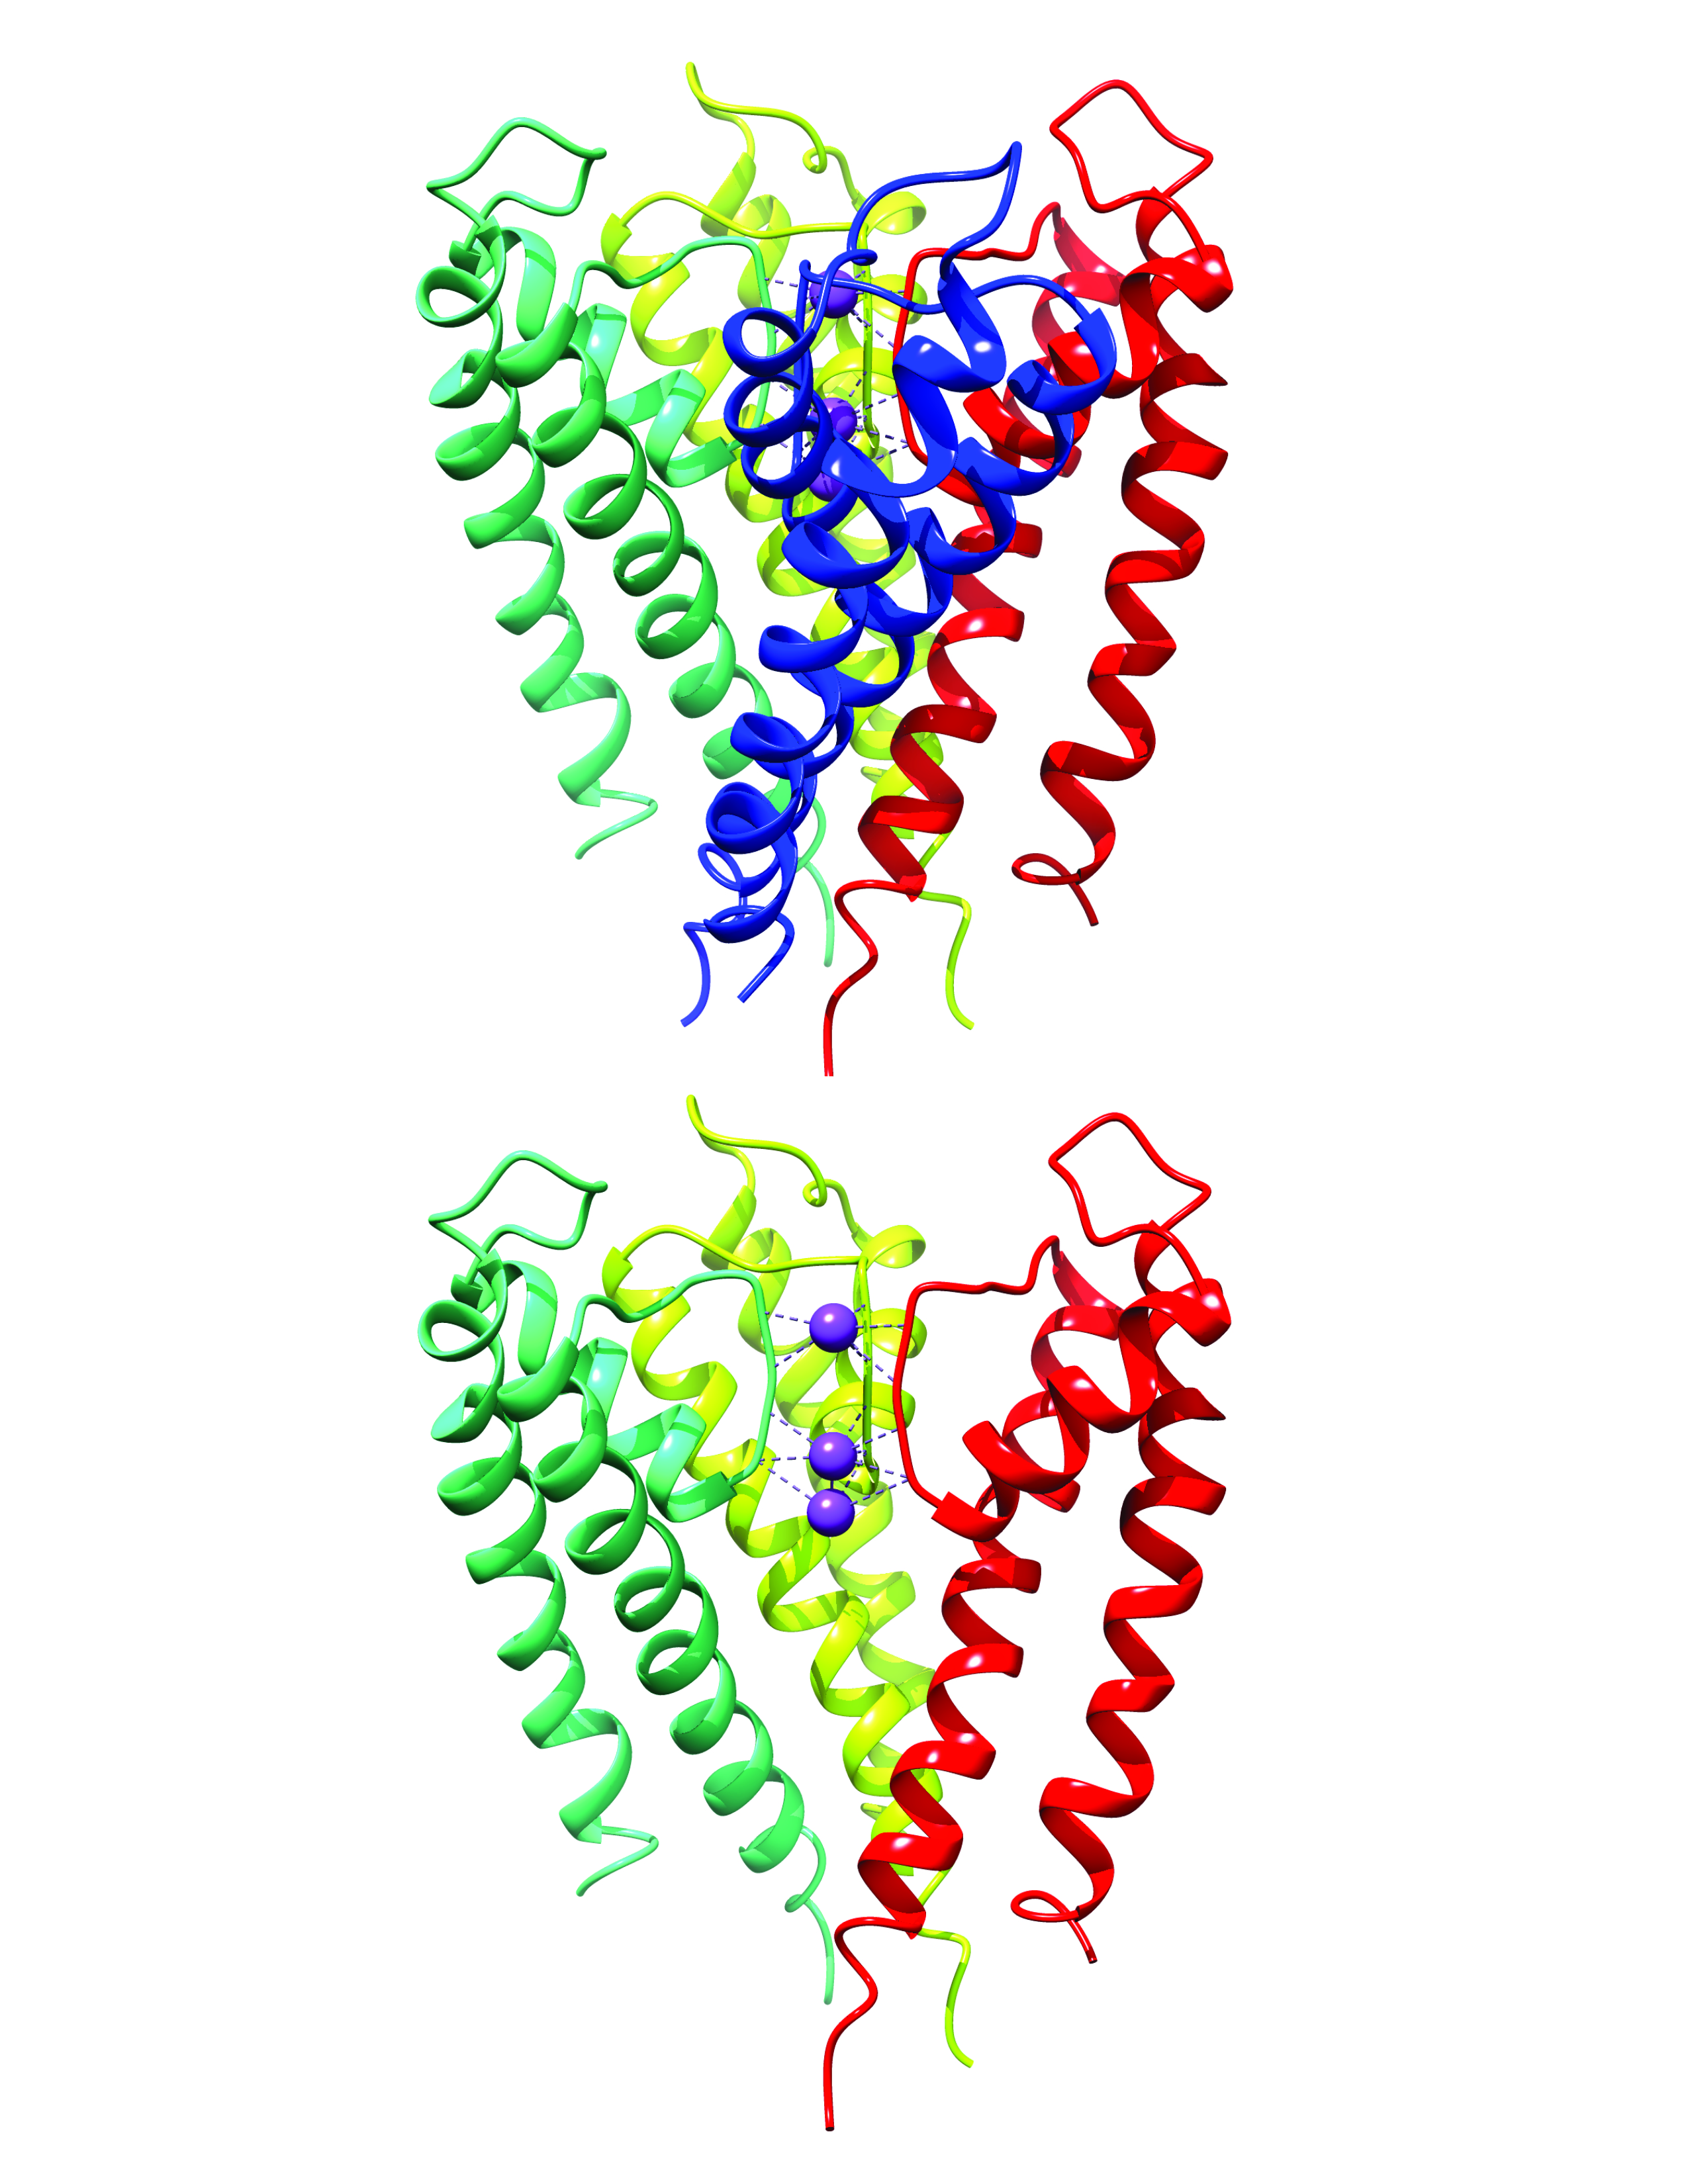
\includegraphics[width=0.7\linewidth]{./figures/potential/Kcsa} 

}

\caption{The structure of the potassium channel KcsA fromn \emph{Streptomyces lividans} determined by X-ray crystallography. KcsA shares sequence similarity with all known K\textsuperscript{+} channels and was the first ion channel to have its structure solved at atomic resolution. It consists of four identical subunits that together form a cone shaped structure (top) with a ion selectivity filter at its outer end. Three K\textsuperscript{+} ions are present in the channel, two of which are helt 7.5 angstroms apart by the selectivity filter, a third K\textsuperscript{+} ion shown in the channel pore below. Molecular graphics were created with \href{http://www.rbvi.ucsf.edu/chimera/}{UCSF Chimera}, developed by the Resource for Biocomputing, Visualization, and Informatics at the University of California, San Francisco, with support from NIH P41-GM103311 used atomic coordinates from \href{https://www.rcsb.org/structure/1BL8}{PDB 1BL8}.}\label{fig:kchannel}
\end{figure}

Because of their small size and the difficulty of crystallizing integral membrane proteins for X-ray analysis, it is only very recently that scientists have been able to directly examine what channels ``look like.'' Most of what researchers have deduced about channel operation so far they have established through electrophysiology, biochemistry, gene sequence comparison and mutagenesisi and structural studies (X-ray crystallography and cryoelectronmicroscopy).

Channels can have single (e.g.~members of the Chloride Intracellular Ion Channel family) or multiple transmembrane (K\textsuperscript{+} channels, P2X receptors, Na\textsuperscript{+} channels) domains which span the plasma membrane to form pores.

Ion channels can be classified by how they respond to their environment. For example, the ion channels involved in the action potential are voltage-sensitive channels; they open and close in response to the voltage across the membrane. Ligand-gated channels form another important class; these ion channels open and close in response to the binding of a ligand molecule, such as a neurotransmitter. Other ion channels open and close with mechanical forces. Still other ion channels---such as those of sensory neurons---open and close in response to other stimuli, such as light, temperature or pressure.

Leakage channels are the simplest type of ion channel, in that their permeability is more or less constant. The types of leakage channels that have the greatest significance in neurons are potassium and chloride channels. Even these are not perfectly constant in their properties: First, most of them are voltage-dependent in the sense that they conduct better in one direction than the other (in other words, they are rectifiers); second, some of them are capable of being shut off by chemical ligands even though they do not require ligands in order to operate.

Also known as ionotropic receptors, ligand-gated ion channels are channels whose permeability is greatly increased when some type of chemical ligand binds to the protein structure. Ligand binding causes a conformational change in the structure of the channel protein that ultimately leads to the opening of the channel gate and subsequent ion flux across the plasma membrane. One example of this type is the AMPA receptor, a receptor for the neurotransmitter glutamate that when activated allows passage of sodium and potassium ions. Another example is the GABA\textsubscript{A} receptor, a receptor for the neurotransmitter GABA that when activated allows passage of chloride ions. Animal cells contain hundreds, if not thousands, of types of these. A large subset function as neurotransmitter receptors---they occur at postsynaptic sites, and the chemical ligand that gates them is released by the presynaptic axon terminal. Ion channels activated by second messengers may also be categorized in this group, although ligands and second messengers are otherwise distinguished from each other.

Voltage-gated ion channels, also known as voltage dependent ion channels, are channels whose permeability is influenced by the membrane potential. They form another very large group, with each member having a particular ion selectivity and a particular voltage dependence. Many are also time-dependent---in other words, they do not respond immediately to a voltage change but only after a delay.

One of the most important members of this group is a type of voltage-gated sodium channel that underlies action potentials---these are sometimes called Hodgkin-Huxley sodium channels because they were initially characterized by Alan Lloyd Hodgkin and Andrew Huxley in their Nobel Prize-winning studies of the physiology of the action potential. The channel is closed at the resting voltage level, but opens abruptly when the voltage exceeds a certain threshold, allowing a large influx of sodium ions that produces a very rapid change in the membrane potential. Recovery from an action potential is partly dependent on a type of voltage-gated potassium channel that is closed at the resting voltage level but opens as a consequence of the large voltage change produced during the action potential.

Important representative families of voltage-gated ion channels are the:

\begin{itemize}
\tightlist
\item
  Voltage-gated sodium channels: This family contains at least 9 members and is largely responsible for action potential creation and propagation. The pore-forming α subunits are very large (up to 4,000 amino acids) and consist of four homologous repeat domains (I-IV) each comprising six transmembrane segments (S1-S6) for a total of 24 transmembrane segments. The members of this family also coassemble with auxiliary β subunits, each spanning the membrane once. Both α and β subunits are extensively glycosylated.
\item
  Voltage-gated calcium channels: This family consists of channels that are formed as a complex of several different subunits: α1, α2δ, β1-4, and γ. The α1 subunit forms the Ca\textsuperscript{2+} selective ion conducting pore while the associated subunits have several functions including modulation of gating.These channels play an important role in both linking muscle excitation with contraction as well as neuronal excitation with transmitter release. The α subunits have an overall structural resemblance to those of the sodium channels and are equally large.
\item
  Cation channels of sperm: This small family of channels, normally referred to as Catsper channels, is related to the two-pore channels and distantly related to TRP channels.
\item
  Voltage-gated potassium channels (KV): This family contains almost 40 members, which are further divided into 12 subfamilies. These channels are known mainly for their role in repolarizing the cell membrane following action potentials. The α subunits have six transmembrane segments, homologous to a single domain of the sodium channels. Correspondingly, they assemble as tetramers to produce a functioning channel.
\item
  Some transient receptor potential channels: This group of channels, normally referred to simply as TRP channels, is named after their role in \emph{Drosophila} phototransduction. This family, containing at least 28 members, is incredibly diverse in its method of activation. Some TRP channels seem to be constitutively open, while others are gated by voltage, intracellular Ca\textsuperscript{2+}, pH, redox state, osmolarity, and mechanical stretch. These channels also vary according to the ion(s) they pass, some being selective for Ca\textsuperscript{2+} while others are less selective, acting as cation channels. This family is subdivided into 6 subfamilies based on homology: classical (TRPC), vanilloid receptors (TRPV), melastatin (TRPM), polycystins (TRPP), mucolipins (TRPML), and ankyrin transmembrane protein 1 (TRPA).
\item
  Hyperpolarization-activated cyclic nucleotide-gated channels: The opening of these channels is due to hyperpolarization rather than the depolarization required for other cyclic nucleotide-gated channels. These channels are also sensitive to the cyclic nucleotides cAMP and cGMP, which alter the voltage sensitivity of the channel's opening. These channels are permeable to the monovalent cations K\textsuperscript{+} and Na\textsuperscript{+}. There are 4 members of this family, all of which form tetramers of six-transmembrane α subunits. As these channels open under hyperpolarizing conditions, they function as pacemaking channels in the heart, particularly the SA node.
\item
  Voltage-gated proton channels: Voltage-gated proton channels open with depolarization, but in a strongly pH-sensitive manner. The result is that these channels open only when the electrochemical gradient is outward, such that their opening will only allow protons to leave cells. Their function thus appears to be acid extrusion from cells. Another important function occurs in phagocytes (e.g.~eosinophils, neutrophils, macrophages) during the ``respiratory burst.'' When bacteria or other microbes are engulfed by phagocytes, the enzyme NADPH oxidase assembles in the membrane and begins to produce reactive oxygen species (ROS) that help kill bacteria. NADPH oxidase is electrogenic, moving electrons across the membrane, and proton channels open to allow proton flux to balance the electron movement electrically.
\end{itemize}

\hypertarget{the-reversal-potential}{%
\section{The Reversal Potential}\label{the-reversal-potential}}

The reversal potential (or equilibrium potential) of an ion is the value of transmembrane voltage at which diffusive and electrical forces counterbalance, so that there is no net ion flow across the membrane. This means that the transmembrane voltage exactly opposes the force of diffusion of the ion, such that the net current of the ion across the membrane is zero and unchanging. The reversal potential is important because it corresponds to the voltage that acts on channels permeable to that ion---in other words, it gives the voltage that the ion concentration gradient generates when it acts as a battery.

The equilibrium potential of a particular ion is usually designated by the notation E\textsubscript{ion}.The equilibrium potential for any ion can be calculated using the Nernst equation. For example, reversal potential for potassium ions will be as follows:

\[  E_{eq,K^+} = \frac{RT}{zF} \ln \frac{[K^+]_{o}}{[K^+]_{i}} \]

where

\begin{itemize}
\tightlist
\item
  E\textsubscript{eq,K\textsuperscript{+}} is the equilibrium potential for potassium, measured in volts
\item
  R is the universal gas constant, equal to 8.314 Joule·K\textsuperscript{−1}·mol\textsuperscript{−1}
\item
  T is the absolute temperature, measured in Kelvin
\item
  z is the number of elementary charges of the ion in question involved in the reaction
\item
  F is the Faraday constant, equal to 96,485 Coulomb·mol\textsuperscript{−1} or J·V\textsuperscript{−1}·mol\textsuperscript{−1}
\item
  {[}K\textsuperscript{+}{]}\textsubscript{o} is the extracellular concentration of potassium, measured in mol·m\textsuperscript{−3} or mmol·l\textsuperscript{−1}
\item
  {[}K\textsuperscript{+}{]}\textsubscript{i} is the intracellular concentration of potassium
\end{itemize}

Even if two different ions have the same charge (i.e., K\textsuperscript{+} and Na\textsuperscript{+}), they can still have very different equilibrium potentials, provided their outside and/or inside concentrations differ. Take, for example, the equilibrium potentials of potassium and sodium in neurons. The potassium equilibrium potential E\textsubscript{K} is −84 mV with 5 mM potassium outside and 140 mM inside. On the other hand, the sodium equilibrium potential, E\textsubscript{Na}, is approximately +66 mV with approximately 12 mM sodium inside and 140 mM outside.

A neuron's resting membrane potential actually changes during the development of an organism. In order for a neuron to eventually adopt its full adult function, its potential must be tightly regulated during development. As an organism progresses through development the resting membrane potential becomes more negative. Glial cells are also differentiating and proliferating as development progresses in the brain. The addition of these glial cells increases the organism's ability to regulate extracellular potassium. The drop in extracellular potassium can lead to a decrease in membrane potential of 35 mV.

Cell excitability is the change in membrane potential that is necessary for cellular responses in various tissues. Cell excitability is a property that is induced during early embriogenesis. Excitability of a cell has also been defined as the ease with which a response may be triggered. The resting potential forms the basis of cell excitability and these processes are fundamental for the generation of graded and action potentials.

The most important regulators of cell excitability are the extracellular calcium concentration and the calcium-sensing receptor. Calcium is also the most important second messenger in excitable cell signaling. Other important proteins that regulate cell excitability are voltage-gated ion channels, ion transporters, membrane receptors and hyperpolarization-activated cyclic-nucleotide-gated channels. For example, potassium channels are important regulators of excitability in neurons, cardiac myocytes and many other excitable cells like astrocytes. Activation of synaptic receptors initiates long-lasting changes in neuronal excitability.

Many cell types are considered to have an excitable membrane. Excitable cells are neurons, cardiac myocytes, skeletal myocytes, smooth muscle cells, many types of endothelial cells (e.g.~beta cells), glial cells (e.g.~astrocytes), mechanoreceptor cells (e.g.~hair cells and Merkel cells), chemoreceptor cells (e.g.~glomus cells, taste receptors), some plant cells and possibly immune cells. Astrocytes display a form of non-electrical excitability based on intracellular calcium variations related to the expression of several receptors through which they can detect the synaptic signal. In neurons, there are different membrane properties in some portions of the cell, for example, dendritic excitability endows neurons with the capacity for coincidence detection of spatially separated inputs.

\hypertarget{the-resting-potential}{%
\section{The Resting Potential}\label{the-resting-potential}}

When the membrane potential of a cell goes for a long period of time without changing significantly, it is referred to as a resting potential or resting voltage. This term is used for the membrane potential of non-excitable cells, but also for the membrane potential of excitable cells in the absence of excitation. In excitable cells, the other possible states are graded membrane potentials (of variable amplitude), and action potentials, which are large, all-or-nothing rises in membrane potential that usually follow a fixed time course. Excitable cells include neurons, muscle cells, and some secretory cells in glands. Even in other types of cells, however, the membrane voltage can undergo changes in response to environmental or intracellular stimuli. For example, depolarization of the plasma membrane appears to be an important step in programmed cell death.

The interactions that generate the resting potential are modeled by the Goldman equation. This is similar in form to the Nernst equation shown above, in that it is based on the charges of the ions in question, as well as the difference between their inside and outside concentrations. However, it also takes into consideration the relative permeability of the plasma membrane to each ion in question.

\[ E_{m} = \frac{RT}{F} \ln{ \left( \frac{ P_{\mathrm{K}}[\mathrm{K}^{+}]_\mathrm{out} + P_{\mathrm{Na}}[\mathrm{Na}^{+}]_\mathrm{out} + P_{\mathrm{Cl}}[\mathrm{Cl}^{-}]_\mathrm{in}}{ P_{\mathrm{K}}[\mathrm{K}^{+}]_\mathrm{in} + P_{\mathrm{Na}}[\mathrm{Na}^{+}]_\mathrm{in} + P_{\mathrm{Cl}}[\mathrm{Cl}^{-}]_\mathrm{out}} \right) } \]

The three ions that appear in this equation are potassium (K\textsuperscript{+}), sodium (Na\textsuperscript{+}), and chloride (Cl\textsuperscript{−}). Calcium is omitted, but can be added to deal with situations in which it plays a significant role. Being an anion, the chloride terms are treated differently from the cation terms; the intracellular concentration is in the numerator, and the extracellular concentration in the denominator, which is reversed from the cation terms. \emph{P\textsubscript{i}} stands for the relative permeability of the ion type \emph{i}.

In essence, the Goldman formula expresses the membrane potential as a weighted average of the reversal potentials for the individual ion types, weighted by permeability. (Although the membrane potential changes about 100 mV during an action potential, the concentrations of ions inside and outside the cell do not change significantly. They remain close to their respective concentrations when the membrane is at resting potential.) In most animal cells, the permeability to potassium is much higher in the resting state than the permeability to sodium. As a consequence, the resting potential is usually close to the potassium reversal potential. The permeability to chloride can be high enough to be significant, but, unlike the other ions, chloride is not actively pumped, and therefore equilibrates at a reversal potential very close to the resting potential determined by the other ions.

Values of resting membrane potential in most animal cells usually vary between the potassium reversal potential (usually around -80 mV) and around -40 mV. The resting potential in excitable cells (capable of producing action potentials) is usually near -60 mV---more depolarized voltages would lead to spontaneous generation of action potentials. Immature or undifferentiated cells show highly variable values of resting voltage, usually significantly more positive than in differentiated cells. In such cells, the resting potential value correlates with the degree of differentiation: undifferentiated cells in some cases may not show any transmembrane voltage difference at all.

Maintenance of the resting potential can be metabolically costly for a cell because of its requirement for active pumping of ions to counteract losses due to leakage channels. The cost is highest when the cell function requires an especially depolarized value of membrane voltage. For example, the resting potential in daylight-adapted blowfly (\emph{Calliphora vicina}) photoreceptors can be as high as -30 mV. This elevated membrane potential allows the cells to respond very rapidly to visual inputs; the cost is that maintenance of the resting potential may consume more than 20\% of overall cellular ATP.

On the other hand, the high resting potential in undifferentiated cells can be a metabolic advantage. This apparent paradox is resolved by examination of the origin of that resting potential. Little-differentiated cells are characterized by extremely high input resistance, which implies that few leakage channels are present at this stage of cell life. As an apparent result, potassium permeability becomes similar to that for sodium ions, which places resting potential in-between the reversal potentials for sodium and potassium as discussed above. The reduced leakage currents also mean there is little need for active pumping in order to compensate, therefore low metabolic cost.

\hypertarget{the-action-potential}{%
\section{The Action Potential}\label{the-action-potential}}

An action potential occurs when the membrane potential of a specific cell location rapidly rises and falls: this depolarisation then causes adjacent locations to similarly depolarise. Action potentials occur in several types of animal cells, called excitable cells, which include neurons, muscle cells, endocrine cells, glomus cells (peripheral chemoreceptor cells mainly located in the carotid and aortic bodies), and in some plant cells.

In neurons, action potentials play a central role in cell-to-cell communication by providing for---or with regard to saltatory conduction, assisting---the propagation of signals along the neuron's axon toward synaptic boutons situated at the ends of an axon; these signals can then connect with other neurons at synapses, or to motor cells or glands. In other types of cells, their main function is to activate intracellular processes. In muscle cells, for example, an action potential is the first step in the chain of events leading to contraction. In beta cells of the pancreas, they provoke release of insulin. Action potentials in neurons are also known as ``nerve impulses'' or ``spikes'', and the temporal sequence of action potentials generated by a neuron is called its ``spike train''. A neuron that emits an action potential, or nerve impulse, is often said to ``fire''.

Action potentials are generated by special types of voltage-gated ion channels embedded in a cell's plasma membrane. These channels are shut when the membrane potential is near the (negative) resting potential of the cell, but they rapidly begin to open if the membrane potential increases to a precisely defined threshold voltage, depolarising the transmembrane potential. When the channels open, they allow an inward flow of sodium ions, which changes the electrochemical gradient, which in turn produces a further rise in the membrane potential. This then causes more channels to open, producing a greater electric current across the cell membrane and so on. The process proceeds explosively until all of the available ion channels are open, resulting in a large upswing in the membrane potential. The rapid influx of sodium ions causes the polarity of the plasma membrane to reverse, and the ion channels then rapidly inactivate. As the sodium channels close, sodium ions can no longer enter the neuron, and they are then actively transported back out of the plasma membrane. Potassium channels are then activated, and there is an outward current of potassium ions, returning the electrochemical gradient to the resting state. After an action potential has occurred, there is a transient negative shift, called the afterhyperpolarization.

In animal cells, there are two primary types of action potentials. One type is generated by voltage-gated sodium channels, the other by voltage-gated calcium channels. Sodium-based action potentials usually last for under one millisecond, but calcium-based action potentials may last for 100 milliseconds or longer. In some types of neurons, slow calcium spikes provide the driving force for a long burst of rapidly emitted sodium spikes. In cardiac muscle cells, on the other hand, an initial fast sodium spike provides a ``primer'' to provoke the rapid onset of a calcium spike, which then produces muscle contraction



\begin{figure}

{\centering 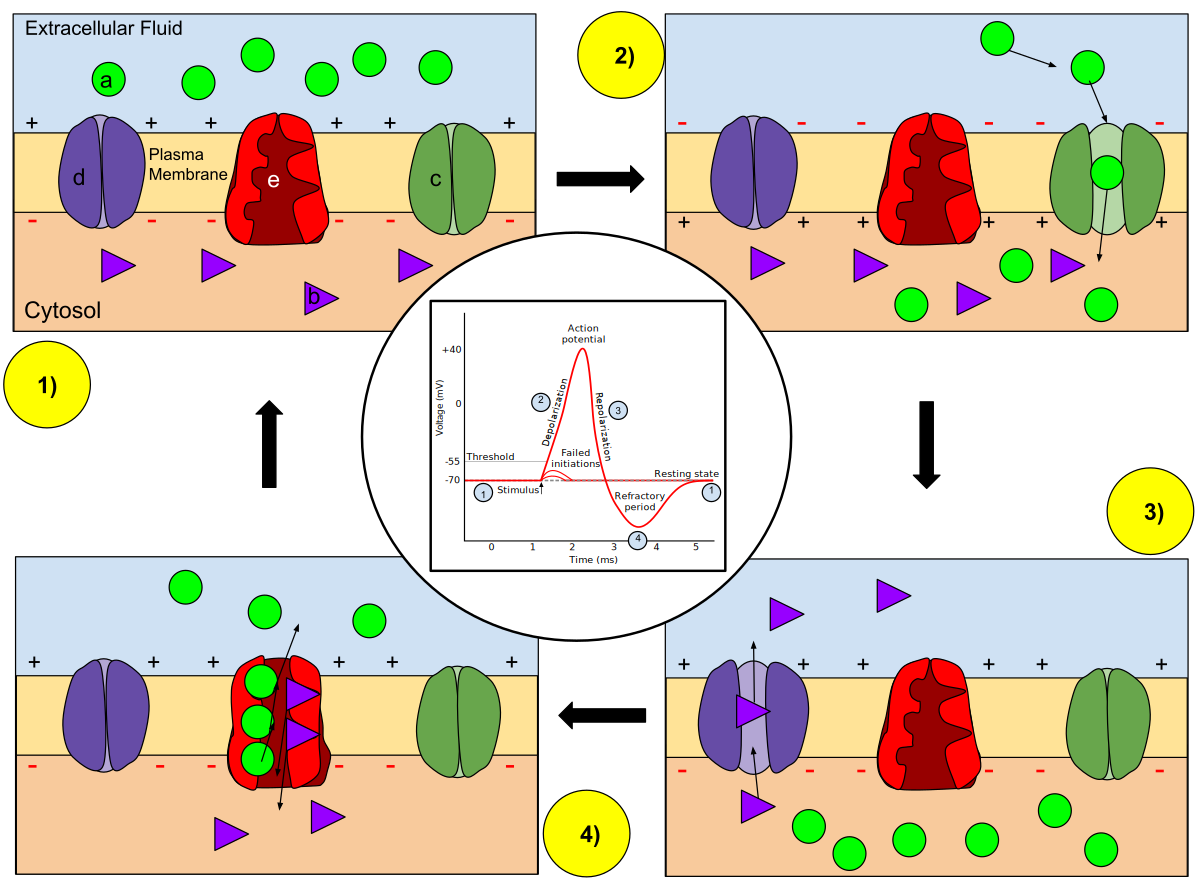
\includegraphics[width=0.7\linewidth]{./figures/potential/ActionPotential} 

}

\caption{\href{https://commons.wikimedia.org/wiki/File:Membrane_Permeability_of_a_Neuron_During_an_Action_Potential.svg}{Ion movement during an action potential.} Key: a) Sodium (Na\textsuperscript{+}) ion. b) Potassium (K\textsuperscript{+}) ion. c) Sodium channel. d) Potassium channel. e) Sodium-potassium pump. In the stages of an action potential, the permeability of the membrane of the neuron changes. At the resting state (1), sodium and potassium ions have limited ability to pass through the membrane, and the neuron has a net negative charge inside. Once the action potential is triggered, the depolarization (2) of the neuron activates sodium channels, allowing sodium ions to pass through the cell membrane into the cell, resulting in a net positive charge in the neuron relative to the extracellular fluid. After the action potential peak is reached, the neuron begins repolarization (3), where the sodium channels close and potassium channels open, allowing potassium ions to cross the membrane into the extracellular fluid, returning the membrane potential to a negative value. Finally, there is a refractory period (4), during which the voltage-dependent ion channels are inactivated while the Na\textsuperscript{+} and K\textsuperscript{+} ions return to their resting state distributions across the membrane (1), and the neuron is ready to repeat the process for the next action potential.}\label{fig:actionpotential}
\end{figure}

\hypertarget{graded-potentials}{%
\section{Graded Potentials}\label{graded-potentials}}

As explained above, the potential at any point in a cell's membrane is determined by the ion concentration differences between the intracellular and extracellular areas, and by the permeability of the membrane to each type of ion. The ion concentrations do not normally change very quickly (with the exception of Ca\textsuperscript{2+}, where the baseline intracellular concentration is so low that even a small influx may increase it by orders of magnitude), but the permeabilities of the ions can change in a fraction of a millisecond, as a result of activation of ligand-gated ion channels. The change in membrane potential can be either large or small, depending on how many ion channels are activated and what type they are, and can be either long or short, depending on the lengths of time that the channels remain open. Changes of this type are referred to as graded potentials, in contrast to action potentials, which have a fixed amplitude and time course.

As can be derived from the Goldman equation shown above, the effect of increasing the permeability of a membrane to a particular type of ion shifts the membrane potential toward the reversal potential for that ion. Thus, opening Na\textsuperscript{+} channels shifts the membrane potential toward the Na\textsuperscript{+} reversal potential, which is usually around +100 mV. Likewise, opening K\textsuperscript{+} channels shifts the membrane potential toward about --90 mV, and opening Cl\textsuperscript{−} channels shifts it toward about --70 mV (resting potential of most membranes). Thus, Na\textsuperscript{+} channels shift the membrane potential in a positive direction, K\textsuperscript{+} channels shift it in a negative direction (except when the membrane is hyperpolarized to a value more negative than the K\textsuperscript{+} reversal potential), and Cl\textsuperscript{−} channels tend to shift it towards the resting potential.

Graded membrane potentials are particularly important in neurons, where they are produced by synapses---a temporary change in membrane potential produced by activation of a synapse by a single graded or action potential is called a postsynaptic potential. Neurotransmitters that act to open Na\textsuperscript{+} channels typically cause the membrane potential to become more positive, while neurotransmitters that activate K\textsuperscript{+} channels typically cause it to become more negative; those that inhibit these channels tend to have the opposite effect.

Whether a postsynaptic potential is considered excitatory or inhibitory depends on the reversal potential for the ions of that current, and the threshold for the cell to fire an action potential (around --50mV). A postsynaptic current with a reversal potential above threshold, such as a typical Na\textsuperscript{+} current, is considered excitatory. A current with a reversal potential below threshold, such as a typical K\textsuperscript{+} current, is considered inhibitory. A current with a reversal potential above the resting potential, but below threshold, will not by itself elicit action potentials, but will produce subthreshold membrane potential oscillations. Thus, neurotransmitters that act to open Na\textsuperscript{+} channels produce excitatory postsynaptic potentials, or EPSPs, whereas neurotransmitters that act to open K\textsuperscript{+} or Cl\textsuperscript{−} channels typically produce inhibitory postsynaptic potentials, or IPSPs. When multiple types of channels are open within the same time period, their postsynaptic potentials summate (are added together).

From the viewpoint of biophysics, the resting membrane potential is merely the membrane potential that results from the membrane permeabilities that predominate when the cell is resting. The Goldman equation of weighted averages always applies, but the following approach may be more easily visualized. At any given moment, there are two factors for an ion that determine how much influence that ion will have over the membrane potential of a cell:

\begin{enumerate}
\def\labelenumi{\arabic{enumi}.}
\tightlist
\item
  That ion's driving force
\item
  That ion's permeability
\end{enumerate}

If the driving force is high, then the ion is being ``pushed'' across the membrane. If the permeability is high, it will be easier for the ion to diffuse across the membrane.

\begin{itemize}
\tightlist
\item
  Driving force is the net electrical force available to move that ion across the membrane. It is calculated as the difference between the voltage that the ion ``wants'' to be at (its equilibrium potential) and the actual membrane potential (E\textsubscript{m}). So, in formal terms, the driving force for an ion = E\textsubscript{m} - E\textsubscript{ion}
\item
  For example, at our earlier calculated resting potential of −73 mV, the driving force on potassium is 7 mV : (−73 mV) − (−80 mV) = 7 mV. The driving force on sodium would be (−73 mV) − (60 mV) = −133 mV.
\item
  Permeability is a measure of how easily an ion can cross the membrane. It is normally measured as the (electrical) conductance and the unit, siemens (S), corresponds to 1 C·s\textsuperscript{−1}·V\textsuperscript{−1}, that is one coulomb per second per volt of potential.
\end{itemize}

So, in a resting membrane, while the driving force for potassium is low, its permeability is very high. Sodium has a huge driving force but almost no resting permeability. In this case, potassium carries about 20 times more current than sodium, and thus has 20 times more influence over E\textsubscript{m} than does sodium.

However, consider another case---the peak of the action potential. Here, permeability to Na is high and K permeability is relatively low. Thus, the membrane moves to near E\textsubscript{Na} and far from E\textsubscript{K}.

\hypertarget{neurotransmission}{%
\chapter{Neurotransmission}\label{neurotransmission}}

Neurotransmission (Latin: transmissio ``passage, crossing'' from transmittere ``send, let through'') is the process by which signaling molecules called neurotransmitters are released by the axon terminal of a neuron (the presynaptic neuron), and bind to and react with the receptors on the dendrites of another neuron (the postsynaptic neuron) a short distance away.

Neurotransmission is regulated by several different factors: the availability and rate-of-synthesis of the neurotransmitter, the release of that neurotransmitter, the baseline activity of the postsynaptic cell, the number of available postsynaptic receptors for the neurotransmitter to bind to, and the subsequent removal or deactivation of the neurotransmitter by enzymes or presynaptic reuptake.

In response to a threshold action potential or graded electrical potential, a neurotransmitter is released at the presynaptic terminal. The released neurotransmitter may then move across the synaptic cleft to bind to receptors in the postsynaptic neuron. Binding of neurotransmitters may influence the postsynaptic neuron in either an inhibitory or excitatory way. The binding of neurotransmitters to receptors in the postsynaptic neuron can trigger either short term changes, such as changes in the membrane potential called postsynaptic potentials, or longer term changes by the activation of signaling cascades.

Neurons form complex biological neural networks through which nerve impulses (action potentials) travel. Neurons do not touch each other (except in the case of an electrical synapse through a gap junction); instead, neurons interact at close contact points called synapses. When the nerve impulse arrives at the synapse, it may cause the release of neurotransmitters, which influence another (postsynaptic) neuron. The postsynaptic neuron may receive inputs from many additional neurons, both excitatory and inhibitory. The excitatory and inhibitory influences are summed, and if the net effect is inhibitory, the neuron will be less likely to ``fire'' (i.e., generate an action potential), and if the net effect is excitatory, the neuron will be more likely to fire. How likely a neuron is to fire depends on how far its membrane potential is from the threshold potential, the voltage at which an action potential is triggered because enough voltage-dependent sodium channels are activated so that the net inward sodium current exceeds all outward currents. Excitatory inputs bring a neuron closer to threshold, while inhibitory inputs bring the neuron farther from threshold. An action potential is an ``all-or-none'' event; neurons whose membranes have not reached threshold will not fire, while those that do must fire. Once the action potential is initiated (traditionally at the axon hillock), it will propagate along the axon, leading to release of neurotransmitters at the synaptic bouton to pass along information to yet another adjacent neuron.

Stages in neurotransmission at the synapse

\begin{itemize}
\tightlist
\item
  Synthesis of the neurotransmitter. This can take place in the cell body, in the axon, or in the axon terminal.
\item
  Storage of the neurotransmitter in storage granules or vesicles in the axon terminal.
\item
  Calcium enters the axon terminal during an action potential, causing release of the neurotransmitter into the synaptic cleft.
\item
  After its release, the transmitter binds to and activates a receptor in the postsynaptic membrane.
\item
  Deactivation of the neurotransmitter. The neurotransmitter is either destroyed enzymatically, or taken back into the terminal from which it came, where it can be reused, or degraded and removed.
\end{itemize}

\hypertarget{the-synapse}{%
\section{The Synapse}\label{the-synapse}}

In the nervous system, a synapse is a structure that permits a neuron (or nerve cell) to pass an electrical or chemical signal to another neuron or to the target effector cell.

Santiago Ramón y Cajal proposed that neurons are not continuous throughout the body, yet still communicate with each other, an idea known as the neuron doctrine. The word ``synapse'' -- from the Greek synapsis (συνάψις), meaning ``conjunction'', in turn from συνάπτεὶν (συν (``together'') and ἅπτειν (``to fasten'')) -- was introduced in 1897 by the English neurophysiologist \href{https://en.wikipedia.org/wiki/Charles_Scott_Sherrington}{Charles Sherrington} in Michael Foster's Textbook of Physiology. Sherrington struggled to find a good term that emphasized a union between two separate elements, and the actual term ``synapse'' was suggested by the English classical scholar Arthur Woollgar Verrall, a friend of Foster. Some authors generalize the concept of the synapse to include the communication from a neuron to any other cell type, such as to a motor cell, although such non-neuronal contacts may be referred to as junctions (a historically older term).A landmark electronmicroscopy study by \href{https://en.wikipedia.org/wiki/Sanford_Palay}{Sanford Palay} demonstrated the existence of synapses. Palay examined thin sections of the abducens nucleus, and on the surfaces of dendrites and cell bodies he encountered clublike profiles that were filled with mitochondria and contained vesicles that were concentrated close to the presynaptic membrane. He also noticed that the pre- and postsynaptic membranes were thickened and appeared denser, and most importantly although these membranes appeared to adhere together, they were in fact separated by a thin intercellular space, the synaptic cleft. This observation directly confirmed Cajal's idea about the synaptic junctions between nerve cells.

Synapses are essential to neuronal function: neurons are cells that are specialized to pass signals to individual target cells, and synapses are the means by which they do so. At a synapse, the plasma membrane of the signal-passing neuron (the presynaptic neuron) comes into close apposition with the membrane of the target (postsynaptic) cell. Both the presynaptic and postsynaptic sites contain extensive arrays of molecular machinery that link the two membranes together and carry out the signaling process. In many synapses, the presynaptic part is located on an axon and the postsynaptic part is located on a dendrite or soma. Astrocytes also exchange information with the synaptic neurons, responding to synaptic activity and, in turn, regulating neurotransmission. Synapses (at least chemical synapses) are stabilized in position by synaptic adhesion molecules (SAMs) projecting from both the pre- and post-synaptic neuron and sticking together where they overlap; SAMs may also assist in the generation and functioning of synapses.



\begin{figure}

{\centering 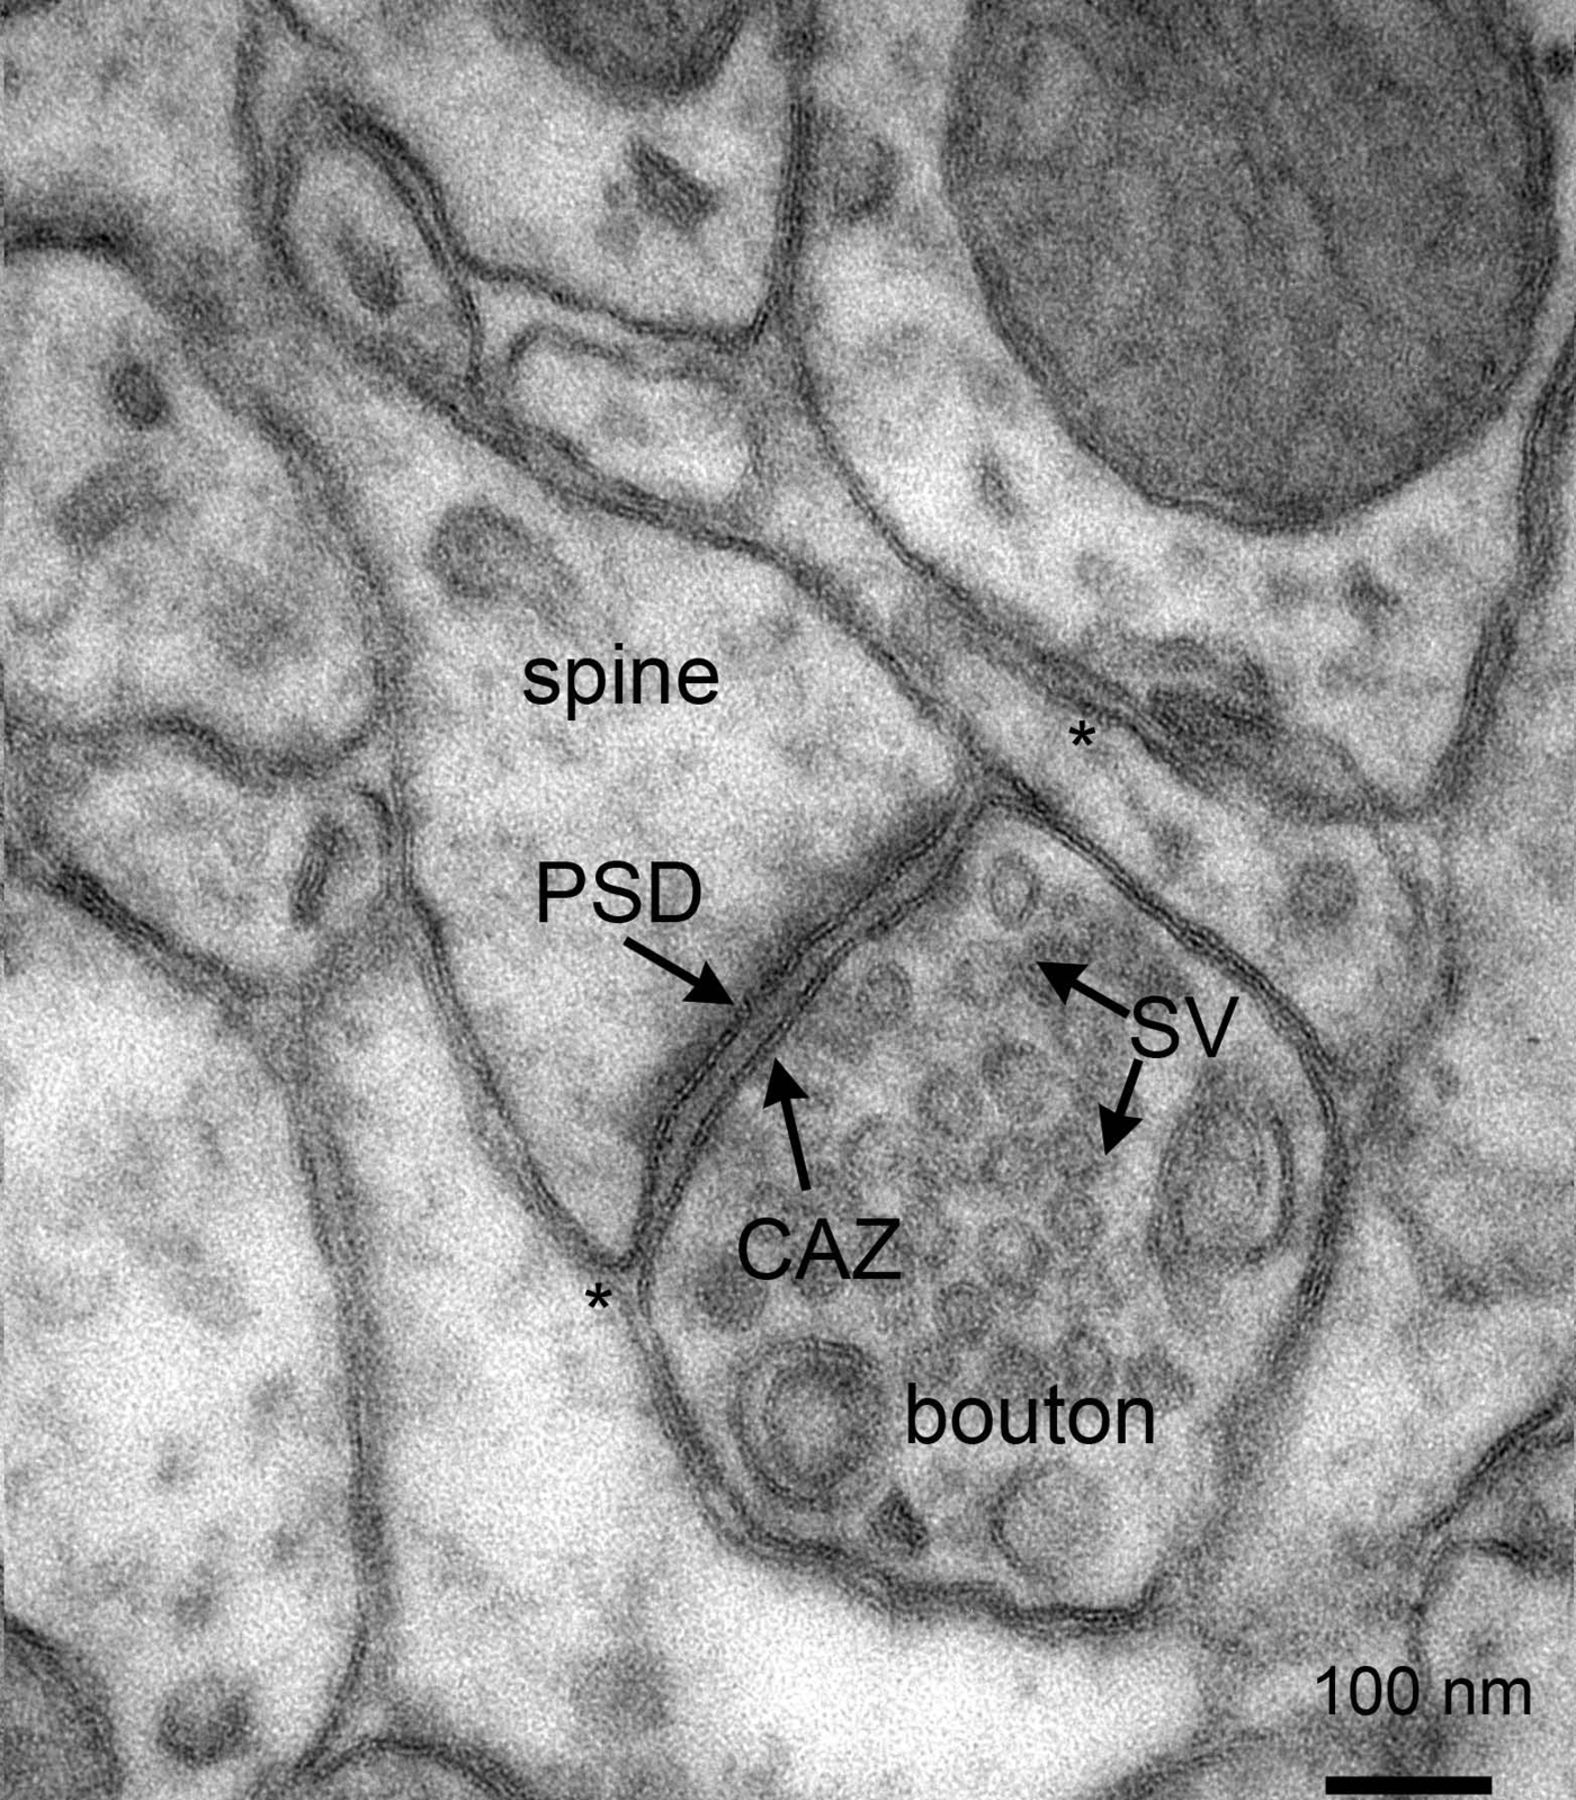
\includegraphics[width=0.7\linewidth]{./figures/synapse/synapse_electronmicrograph} 

}

\caption{Electron micrograph of rat cortex showing multiple pre- and postsynaptic structures, as well as astrocytic endfeet (*) in close contact with synapses. Note the presence of numerous synaptic vesicles in the presynaptic boutons. CAZ, cytomatrix at the active zone; PSD, postsynaptic density; SV, synaptic vesicles. Scalebar: 100 nm. From \href{https://doi.org/10.1074/mcp.R115.051482}{Proteomics of the Synapse -- A Quantitative Approach to Neuronal Plasticity Daniela C. Dieterich, Michael R. Kreutz Molecular \& Cellular Proteomics February 1, 2016, First published on August 25, 2015, 15 (2) 368-381; DOI: 10.1074/mcp.R115.051482}}\label{fig:electronsynapse}
\end{figure}

There are two fundamentally different types of synapses:

\begin{itemize}
\tightlist
\item
  In a chemical synapse, electrical activity in the presynaptic neuron is converted (via the activation of voltage-gated calcium channels) into the release of a chemical called a neurotransmitter that binds to receptors located in the plasma membrane of the postsynaptic cell. The neurotransmitter may initiate an electrical response or a secondary messenger pathway that may either excite or inhibit the postsynaptic neuron. Chemical synapses can be classified according to the neurotransmitter released: glutamatergic (often excitatory), GABAergic (often inhibitory), cholinergic (e.g.~vertebrate neuromuscular junction), and adrenergic (releasing norepinephrine). Because of the complexity of receptor signal transduction, chemical synapses can have complex effects on the postsynaptic cell.
\item
  In an electrical synapse, the presynaptic and postsynaptic cell membranes are connected by special channels called gap junctions that are capable of passing an electric current, causing voltage changes in the presynaptic cell to induce voltage changes in the postsynaptic cell. The main advantage of an electrical synapse is the rapid transfer of signals from one cell to the next.
\end{itemize}

An autapse is a chemical or electrical synapse that forms when the axon of one neuron synapses onto dendrites of the same neuron.

Synapses can be classified by the type of cellular structures serving as the pre- and post-synaptic components. The vast majority of synapses in the mammalian nervous system are classical axo-dendritic synapses (axon synapsing upon a dendrite), however, a variety of other arrangements exist. These include but are not limited to axo-axonic, dendro-dendritic, axo-secretory, somato-dendritic, dendro-somatic, and somato-somatic synapses.

The axon can synapse onto a dendrite, onto a cell body, or onto another axon or axon terminal, as well as into the bloodstream or diffusely into the adjacent nervous tissue.

The postsynaptic density (PSD) is a protein dense specialization attached to the postsynaptic membrane. PSDs were originally identified by electron microscopy as an electron-dense region at the membrane of a postsynaptic neuron. The PSD is in close apposition to the presynaptic active zone and ensures that receptors are in close proximity to presynaptic neurotransmitter release sites. PSDs vary in size and composition among brain regions and have been studied in great detail at glutamatergic synapses. Hundreds of proteins have been identified in the postsynaptic density including glutamate receptors, scaffold proteins, and many signaling molecules.

PSDs are sized on the order of 250 to 500 nanometres in diameter and 25 to 50 nanometres in thickness, depending on the activity state of the synapse. During synaptic plasticity, the total size of the PSD is increasing along with an increase in synaptic size and strength after inducing long-term potentiation at single synapses.

Many proteins in the PSD are involved in the regulation of synaptic function. Key among these, are postsynaptic density-95 (PSD95), neuroligin (a cellular adhesion molecule), NMDA receptors, AMPA receptors, calcium/calmodulin-dependent protein kinase II and actin. As protein detection technologies have increased in sensitivity, such as with improvements in mass spectrometry techniques, many more proteins have been found to be part of the PSD. Current estimates are that several hundred proteins are found at PSDs in different brain regions and during different states of development and synaptic activity. PSDs also contain cell adhesion molecules and a diverse set of other signaling proteins. Many of the PSD proteins contain PDZ domains.

The PSD has been proposed to concentrate and organize neurotransmitter receptors in the synaptic cleft. The PSD also serves as a signaling apparatus. For instance kinases and phosphatases in the PSD are activated and released from the PSD to change the activity of proteins located in the spine or are transported to the nucleus to affect protein synthesis. Some of the features of the PSD are similar to the neuromuscular junction and other cellular junctions, as the PSD has been modeled as a specialized cellular junction that allows for rapid, asymmetrical signaling.



\begin{figure}

{\centering 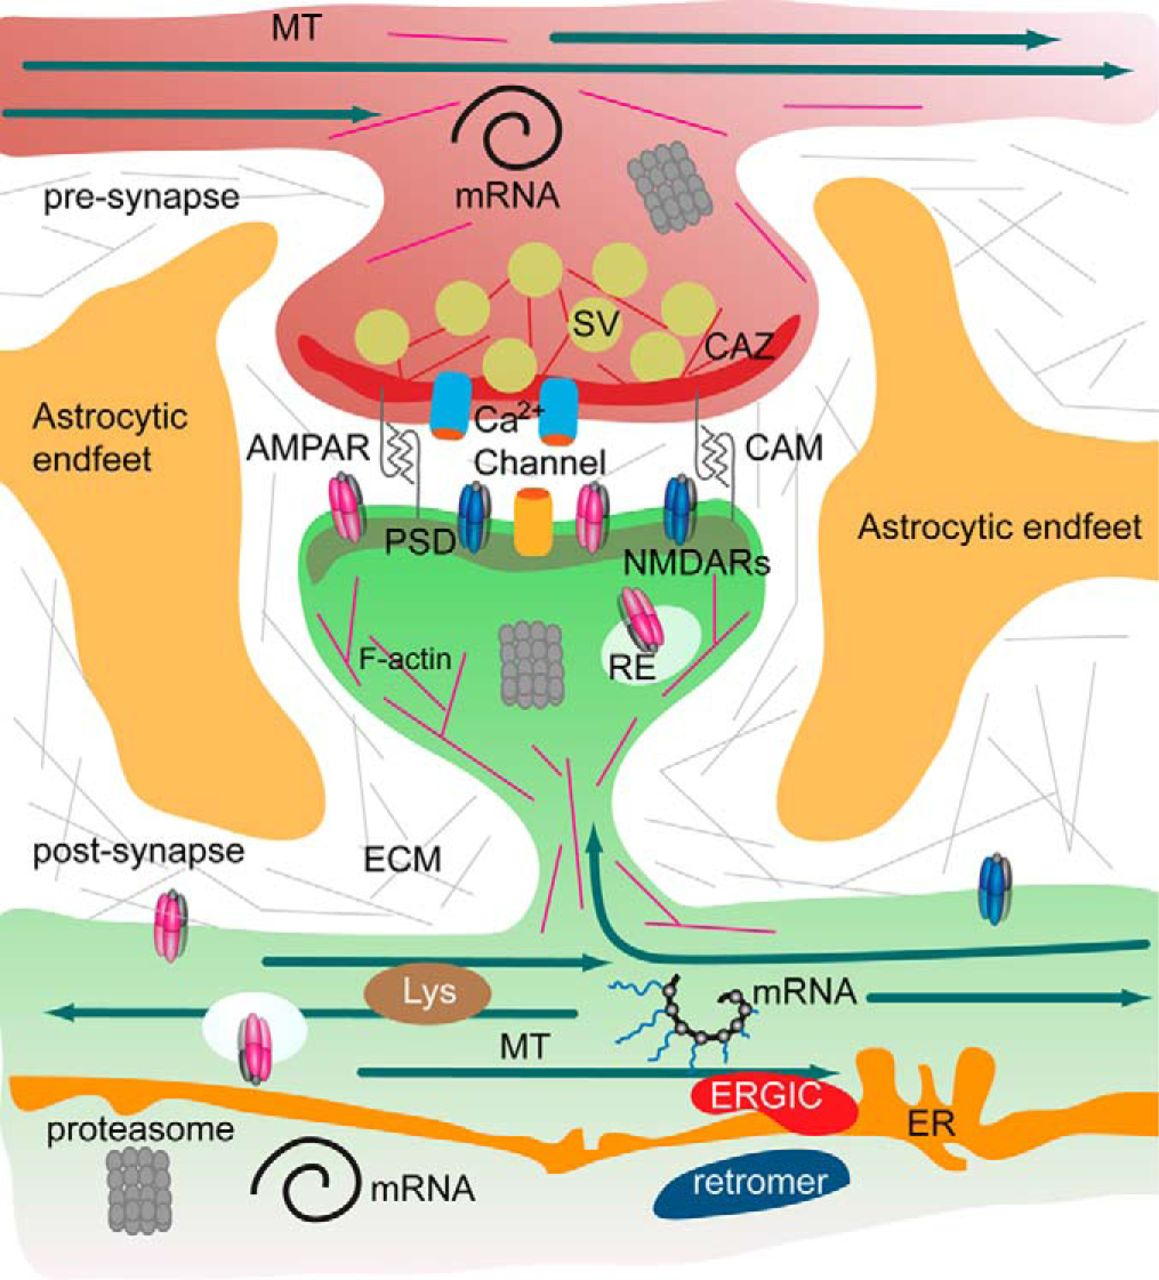
\includegraphics[width=0.7\linewidth]{./figures/synapse/synapse_diagram} 

}

\caption{The tetrapartite synapse of principal neurons in the forebrain, consisting of the pre- and postsynaptic compartment, astrocytic endfeet, and the extracellular matrix has a tightly regulated protein composition. A microsceretory system is present in synapses and dendrites that allows for translation of mRNA, local synthesis of, processing and insertion of transmembrane proteins. Hence the turnover of the synaptic protein machinery is controlled by local and somatic de novo protein synthesis, protein degradation by the ubiquitin proteasome system, lysosomes and autophagosomes. In addition, the association of proteins with pre- and postsynaptic compartments is highly dynamic. Molecular machineries and organelles for proteostasis are shared between synapses in dendritic segments. Proteins are transported in and out of the synapse as well as by diffusion of transmembrane proteins. These processes govern the activity-dependent assembly of the pre- and postsynaptic scaffold and the synaptic surface expression of receptors, calcium channels and cell adhesion molecules. Abbreviations: CAM, cell adhesion molecules; CAZ, cytomatrix at the active zone; ECM, extracellular matrix; ER, endoplasmatic reticulum; ERGIC, endoplasmatic reticulum Golgi intermediate compartment; MT, microtubules; PSD, postsynaptic density; RE, recycling endosomes; Lys, lysomes; SV, synaptic vesicle. From \href{https://doi.org/10.1074/mcp.R115.051482}{Proteomics of the Synapse -- A Quantitative Approach to Neuronal Plasticity Daniela C. Dieterich, Michael R. Kreutz Molecular \& Cellular Proteomics February 1, 2016, First published on August 25, 2015, 15 (2) 368-381; DOI: 10.1074/mcp.R115.051482}}\label{fig:synapsediagram}
\end{figure}

The adult human brain is estimated to contain from 10\textsuperscript{14} to 5 × 10\textsuperscript{14} (100--500 trillion) synapses. Every cubic millimeter of cerebral cortex contains roughly a billion (10\textsuperscript{9}) of them. The number of synapses in the human cerebral cortex has separately been estimated at 0.15 quadrillion (150 trillion)

It is widely accepted that the synapse plays a role in the formation of memory. As neurotransmitters activate receptors across the synaptic cleft, the connection between the two neurons is strengthened when both neurons are active at the same time, as a result of the receptor's signaling mechanisms. The strength of two connected neural pathways is thought to result in the storage of information, resulting in memory. This process of synaptic strengthening is known as long-term potentiation.

Synaptic transmission can be changed by previous activity. These changes are called synaptic plasticity and may result in either a decrease in the efficacy of the synapse, called depression, or an increase in efficacy, called potentiation. These changes can either be long-term or short-term. Forms of short-term plasticity include synaptic fatigue or depression and synaptic augmentation. Forms of long-term plasticity include long-term depression and long-term potentiation. Synaptic plasticity can be either homosynaptic (occurring at a single synapse) or heterosynaptic (occurring at multiple synapses).

By altering the release of neurotransmitters, the plasticity of synapses can be controlled in the presynaptic cell. The postsynaptic cell can be regulated by altering the function and number of its receptors. Changes in postsynaptic signaling are most commonly associated with a N-methyl-D-aspartic acid receptor (NMDAR)-dependent long-term potentiation (LTP) and long-term depression (LTD) due to the influx of calcium into the post-synaptic cell, which are the most analyzed forms of plasticity at excitatory synapses.

A neurotransmitter can influence the function of a neuron through a remarkable number of mechanisms. In its direct actions in influencing a neuron's electrical excitability, however, a neurotransmitter acts in only one of two ways: excitatory or inhibitory. A neurotransmitter influences trans-membrane ion flow either to increase (excitatory) or to decrease (inhibitory) the probability that the cell with which it comes in contact will produce an action potential. Thus, despite the wide variety of synapses, they all convey messages of only these two types, and they are labeled as such. Type I synapses are excitatory in their actions, whereas type II synapses are inhibitory. Each type has a different appearance and is located on different parts of the neurons under its influence.

Type I (excitatory) synapses are typically located on the shafts or the spines of dendrites, whereas type II (inhibitory) synapses are typically located on a cell body. In addition, Type I synapses have round synaptic vesicles, whereas the vesicles of type II synapses are flattened. The material on the presynaptic and post-synaptic membranes is denser in a Type I synapse than it is in a type II, and the type I synaptic cleft is wider. Finally, the active zone on a Type I synapse is larger than that on a Type II synapse.

The different locations of type I and type II synapses divide a neuron into two zones: an excitatory dendritic tree and an inhibitory cell body. From an inhibitory perspective, excitation comes in over the dendrites and spreads to the axon hillock to trigger an action potential. If the message is to be stopped, it is best stopped by applying inhibition on the cell body, close to the axon hillock where the action potential originates.

Here is a summary of the sequence of events that take place in synaptic transmission from a presynaptic neuron to a postsynaptic cell. Each step is explained in more detail below. Note that with the exception of the final step, the entire process may run only a few hundred microseconds, in the fastest synapses.

\begin{itemize}
\tightlist
\item
  The process begins with an action potential traveling along the membrane of the presynaptic cell, until it reaches the synapse.
\item
  The electrical depolarization of the membrane at the synapse causes channels to open that are permeable to calcium ions.
\item
  Calcium ions flow through the presynaptic membrane, rapidly increasing the calcium concentration in the interior.
\item
  The high calcium concentration activates a set of calcium-sensitive proteins attached to vesicles that contain a neurotransmitter chemical.
\item
  These proteins change shape, causing the membranes of some ``docked'' vesicles to fuse with the membrane of the presynaptic cell, thereby opening the vesicles and dumping their neurotransmitter contents into the synaptic cleft, the narrow space between the membranes of the pre- and postsynaptic cells.
\item
  The neurotransmitter diffuses within the cleft. Some of it escapes, but some of it binds to chemical receptor molecules located on the membrane of the postsynaptic cell.
\item
  The binding of neurotransmitter causes the receptor molecule to be activated.
\item
  Due to thermal vibration, the motion of atoms, vibrating about their equilibrium positions in a crystalline solid, neurotransmitter molecules eventually break loose from the receptors and drift away.
\item
  The neurotransmitter is either reabsorbed by the presynaptic cell, and then repackaged for future release, or else it is broken down metabolically.
\end{itemize}

In general, if an excitatory synapse is strong enough, an action potential in the presynaptic neuron will trigger an action potential in the postsynaptic cell. In many cases the excitatory postsynaptic potential (EPSP) will not reach the threshold for eliciting an action potential. When action potentials from multiple presynaptic neurons fire simultaneously, or if a single presynaptic neuron fires at a high enough frequency, the EPSPs can overlap and summate. If enough EPSPs overlap, the summated EPSP can reach the threshold for initiating an action potential. This process is known as summation.

On the other hand, a presynaptic neuron releasing an inhibitory neurotransmitter, such as GABA, can cause an inhibitory postsynaptic potential (IPSP) in the postsynaptic neuron, moving the membrane potential farther away from the threshold, decreasing its excitability and making it more difficult for the neuron to initiate an action potential. If an IPSP overlaps with an EPSP, the IPSP can in many cases prevent the neuron from firing an action potential. In this way, the output of a neuron may depend on the input of many different neurons, each of which may have a different degree of influence, depending on the strength and type of synapse with that neuron. \href{https://en.wikipedia.org/wiki/John_Eccles_(neurophysiologist)}{John Carew Eccles} performed some of the important early experiments on synaptic integration, for which he received the Nobel Prize for Physiology or Medicine in 1963.

Understanding the effects of drugs on neurotransmitters comprises a significant portion of research initiatives in the field of neuroscience. Most neuroscientists involved in this field of research believe that such efforts may further advance our understanding of the circuits responsible for various neurological diseases and disorders, as well as ways to effectively treat and someday possibly prevent or cure such illnesses.

\hypertarget{neurotransmitters}{%
\section{Neurotransmitters}\label{neurotransmitters}}

Neurotransmitters are endogenous chemicals that enable neurotransmission. It is a type of chemical messenger which transmits signals across a chemical synapse, such as a neuromuscular junction, from one neuron (nerve cell) to another ``target'' neuron, muscle cell, or gland cell. Neurotransmitters are released from synaptic vesicles in synapses into the synaptic cleft, where they are received by neurotransmitter receptors on the target cells. Many neurotransmitters are synthesized from simple and plentiful precursors such as amino acids, which are readily available from the diet and only require a small number of biosynthetic steps for conversion. Neurotransmitters play a major role in shaping everyday life and functions. Their exact numbers are unknown, but more than 200 unique chemical messengers have been identified.

Neurotransmitters are stored in synaptic vesicles, clustered close to the cell membrane at the axon terminal of the presynaptic neuron. Neurotransmitters are released into and diffuse across the synaptic cleft, where they bind to specific receptors on the membrane of the postsynaptic neuron.

Neurotransmitter action is terminated in three different ways:

\begin{itemize}
\tightlist
\item
  Diffusion -- the neurotransmitter detaches from receptor, drifting out of the synaptic cleft, here it becomes absorbed by glial cells.
\item
  Enzyme degradation -- special chemicals called enzymes break it down. Usually, astrocytes absorb the excess neurotransmitters and pass them on to enzymes or pump them directly into the presynaptic neuron.
\item
  Reuptake -- re-absorption of a neurotransmitter into the neuron. Transporters, or membrane transport proteins, pump neurotransmitters from the synaptic cleft back into axon terminals (the presynaptic neuron) where they are stored.
\end{itemize}

For example, choline is taken up and recycled by the pre-synaptic neuron to synthesize more ACh. Other neurotransmitters such as dopamine are able to diffuse away from their targeted synaptic junctions and are eliminated from the body via the kidneys, or destroyed in the liver. Each neurotransmitter has very specific degradation pathways at regulatory points, which may be targeted by the body's regulatory system or by recreational drugs.

Until the early 20th century, scientists assumed that the majority of synaptic communication in the brain was electrical. But in 1921 German pharmacologist \href{https://en.wikipedia.org/wiki/Otto_Loewi}{Otto Loewi} (1873--1961) demonstrated that neurons can communicate by releasing chemicals. Some neurons do, however, communicate via electrical synapses through the use of gap junctions, which allow specific ions to pass directly from one cell to another.

There are four classical criteria for identifying neurotransmitters:

\begin{enumerate}
\def\labelenumi{\arabic{enumi}.}
\tightlist
\item
  The chemical must be synthesized in the neuron or otherwise be present in it.
\item
  When the neuron is active, the chemical must be released and produce a response in some target.
\item
  The same response must be obtained when the chemical is experimentally placed on the target.
\item
  A mechanism must exist for removing the chemical from its site of activation after its work is done.
\end{enumerate}

The anatomical localization of neurotransmitters is typically determined using immunocytochemical techniques, which identify the location of either the transmitter substances themselves, or of the enzymes that are involved in their synthesis. Immunocytochemical techniques have also revealed that many transmitters, particularly the neuropeptides, are co-localized, that is, one neuron may release more than one transmitter from its synaptic terminal. Various techniques have been used to identify neurotransmitters throughout the central nervous system.

There are many different ways to classify neurotransmitters. Dividing them into amino acids, peptides, and monoamines is sufficient for some classification purposes.

Major neurotransmitters:

\begin{itemize}
\tightlist
\item
  Amino acids: glutamate, aspartate, D-serine, γ-aminobutyric acid (GABA), glycine
\item
  Gasotransmitters: nitric oxide (NO), carbon monoxide (CO), hydrogen sulfide (H\textsubscript{2}S)
\item
  Monoamines: dopamine (DA), norepinephrine (noradrenaline; NE, NA), epinephrine (adrenaline), histamine, serotonin (SER, 5-HT)
\item
  Trace amines: phenethylamine, N-methylphenethylamine, tyramine, 3-iodothyronamine, octopamine, tryptamine, etc.
\item
  Peptides: oxytocin, somatostatin, substance P, cocaine and amphetamine regulated transcript, opioid peptides
\item
  Purines: adenosine triphosphate (ATP), adenosine
\item
  Catecholamines: dopamine, norepinephrine (noradrenaline), epinephrine (adrenaline)
\item
  Others: acetylcholine (ACh), anandamide, etc.
\end{itemize}

In addition, over 50 neuroactive peptides have been found, and new ones are discovered regularly. Many of these are ``co-released'' along with a small-molecule transmitter. Nevertheless, in some cases a peptide is the primary transmitter at a synapse. β-endorphin is a relatively well-known example of a peptide neurotransmitter because it engages in highly specific interactions with opioid receptors in the central nervous system.

Single ions (such as synaptically released zinc) are also considered neurotransmitters by some, as well as some gaseous molecules such as nitric oxide (NO), carbon monoxide (CO), and hydrogen sulfide (H\textsubscript{2}S).

The most prevalent transmitter is glutamate, which is excitatory at well over 90\% of the synapses in the human brain. The next most prevalent is Gamma-Aminobutyric Acid, or GABA, which is inhibitory at more than 90\% of the synapses that do not use glutamate. Although other transmitters are used in fewer synapses, they may be very important functionally: the great majority of psychoactive drugs exert their effects by altering the actions of some neurotransmitter systems, often acting through transmitters other than glutamate or GABA. Addictive drugs such as cocaine and amphetamines exert their effects primarily on the dopamine system. The addictive opiate drugs exert their effects primarily as functional analogs of opioid peptides, which, in turn, regulate dopamine levels.

\hypertarget{modulatory-neurotransmitter-systems}{%
\subsection{Modulatory Neurotransmitter Systems}\label{modulatory-neurotransmitter-systems}}

Neurons expressing certain types of neurotransmitters sometimes form distinct systems, where activation of the system acts in a modulatory fashion on a large number of neurons in large volumes of the brain. Such modulatory neurotransmitter systems include the noradrenaline (norepinephrine) system, the dopamine system, the serotonin system, and the cholinergic system, among others. Neuromodulatory neurotransmitters typically bind to metabotropic, G-protein coupled receptors to initiate a second messenger signaling cascade that induces a broad, long-lasting signal. This modulation can last for hundreds of milliseconds to several minutes. Some of the effects of neuromodulators include: altering the intrinsic firing activity, increasing or decreasing voltage-dependent currents, changing synaptic efficacy, increasing bursting activity and reconfiguring of synaptic connectivity.

\begin{longtable}[t]{>{\raggedright\arraybackslash}p{5em}>{\raggedright\arraybackslash}p{15em}>{\raggedright\arraybackslash}p{10em}>{\raggedright\arraybackslash}p{15em}}
\caption{\label{tab:modulators}Major modulatory neurotransmitter systems}\\
\toprule
System & Origin & Targets & Effects\\
\midrule
\rowcolor{gray!6}   &  & Adrenergic receptors in: & arousal,  reward system\\

 &  & spinal cord & \\

\rowcolor{gray!6}   &  & thalamus & \\

 &  & hypothalamus & \\

\rowcolor{gray!6}   &  & striatum & \\

 &  & neocortex & \\

\rowcolor{gray!6}   &  & cingulate gyrus & \\

 &  & cingulum & \\

\rowcolor{gray!6}   &  & hippocampus & \\

 & \multirow{-10}{15em}{\raggedright\arraybackslash Locus coeruleus} & amygdala & \\

\rowcolor{gray!6}  \multirow{-11}{5em}{\raggedright\arraybackslash Noradrenaline system} & Lateral tegmental field & hypothalamus & \\
\cmidrule{1-4}
 & Dopamine pathways: & Dopamine receptors at pathway terminations. & motor system, reward system, cognition, endocrine, nausea\\

\rowcolor{gray!6}   & mesocortical pathway &  & \\

 & mesolimbic pathway &  & \\

\rowcolor{gray!6}   & nigrostriatal pathway &  & \\

\multirow{-5}{5em}{\raggedright\arraybackslash Dopamine system} & tuberoinfundibular pathway &  & \\
\cmidrule{1-4}
\rowcolor{gray!6}   &  & Serotonin receptors in: deep cerebellar nuclei, cerebellar cortex, spinal cord & increase (introversion): mood, satiety, body temperature, sleep;  decrease: nociception\\

Serotonin system & caudal dorsal raphe nucleus &  \vphantom{2} & \\
\rowcolor{gray!6}  Serotonin system & caudal dorsal raphe nucleus &  \vphantom{1} & \\
 &  &  & \\

\rowcolor{gray!6}  Serotonin system & rostral dorsal raphe nucleus &  \vphantom{1} & \\
 &  &  & \\

\rowcolor{gray!6}   &  & Serotonin receptors in: & \\

 &  & thalamus & \\

\rowcolor{gray!6}   &  & striatum & \\

 &  & hypothalamus & \\

\rowcolor{gray!6}   &  & nucleus accumbens & \\

 &  & neocortex & \\

\rowcolor{gray!6}   &  & cingulate gyrus & \\

 &  & cingulum & \\

\rowcolor{gray!6}   &  & hippocampus & \\

\multirow{-16}{5em}{\raggedright\arraybackslash Serotonin system} & \multirow{-12}{15em}{\raggedright\arraybackslash rostral dorsal raphe nucleus} & amygdala & \\
\cmidrule{1-4}
\rowcolor{gray!6}   &  & (mainly) M1 receptors in: & muscle and motor control system, learning, short-term memory, arousal, reward\\

 &  & brainstem & \\

\rowcolor{gray!6}   &  & deep cerebellar nuclei & \\

 &  & pontine nuclei & \\

\rowcolor{gray!6}   &  & locus ceruleus & \\

 &  & raphe nucleus & \\

\rowcolor{gray!6}   &  & lateral reticular nucleus & \\

 &  & inferior olive & \\

\rowcolor{gray!6}   &  & thalamus & \\

 &  & tectum & \\

\rowcolor{gray!6}   &  & basal ganglia & \\

 & \multirow{-12}{15em}{\raggedright\arraybackslash Pedunculopontine nucleus and dorsolateral tegmental nuclei(pontomesencephalotegmental complex)} & basal forebrain & \\

\rowcolor{gray!6}   &  & (mainly) M1 receptors in: & \\

 & \multirow{-2}{15em}{\raggedright\arraybackslash basal optic nucleus of Meynert} & neocortex & \\

\rowcolor{gray!6}   &  & (mainly) M1 receptors in: & \\

 &  & hippocampus & \\

\rowcolor{gray!6}  \multirow{-17}{5em}{\raggedright\arraybackslash Cholinergic system} & \multirow{-3}{15em}{\raggedright\arraybackslash medial septal nucleus} & neocortex & \\
\bottomrule
\end{longtable}

\hypertarget{neurotransmitter-receptors}{%
\section{Neurotransmitter Receptors}\label{neurotransmitter-receptors}}

There are two major types of neurotransmitter receptors: ionotropic and metabotropic. Ionotropic means that ions can pass through the receptor, whereas metabotropic means that a second messenger inside the cell relays the message (i.e.~metabotropic receptors do not have channels). Metabotropic receptors are G-protein-coupled receptors (GPCRs). Ionotropic receptors are also called ligand-gated ion channels. Conversely, GPCRs are neither excitatory nor inhibitory. Rather, they can have a broad number of functions such as modulating the actions of excitatory and inhibitory ion channels or triggering a signalling cascade that releases calcium from stores inside the cell.

\hypertarget{ionotropic-receptors-neurotransmitter-gated-ion-channels}{%
\subsection{Ionotropic Receptors: Neurotransmitter-Gated Ion Channels}\label{ionotropic-receptors-neurotransmitter-gated-ion-channels}}

Ligand-gated ion channels (LGICs) are one type of ionotropic receptor or channel-linked receptor. They are a group of transmembrane ion channels that are opened or closed in response to the binding of a chemical messenger (i.e., a ligand), such as a neurotransmitter.

The binding site of endogenous ligands on LGICs protein complexes are normally located on a different portion of the protein (an allosteric binding site) compared to where the ion conduction pore is located. The direct link between ligand binding and opening or closing of the ion channel, which is characteristic of ligand-gated ion channels, is contrasted with the indirect function of metabotropic receptors, which use second messengers. LGICs are also different from voltage-gated ion channels (which open and close depending on membrane potential), and stretch-activated ion channels (which open and close depending on mechanical deformation of the cell membrane).

\hypertarget{metabotropic-receptors-g-protein-coupled-receptors}{%
\subsection{Metabotropic Receptors: G-Protein Coupled Receptors}\label{metabotropic-receptors-g-protein-coupled-receptors}}

GPCRs also known as seven-transmembrane domain receptors, 7TM receptors, heptahelical receptors, serpentine receptor comprise a large protein family of transmembrane receptors that sense molecules outside the cell and activate intracellular signal transduction pathways. GPCRs are found only in eukaryotes. The ligands that bind and activate these receptors include light-sensitive compounds, odors, pheromones, hormones, and neurotransmitters, and vary in size from small molecules to peptides to large proteins. G protein-coupled receptors are involved in many diseases, and are also the target of approximately 30\% of all modern medicinal drugs.

There are two principal signal transduction pathways involving the G protein-coupled receptors: the cAMP signal pathway and the phosphatidylinositol signal pathway. When a ligand binds to the GPCR it causes a conformational change in the GPCR, which allows it to act as a guanine nucleotide exchange factor (GEF). The GPCR can then activate an associated G-protein by exchanging its bound GDP for a GTP. The G-protein's α subunit, together with the bound GTP, can then dissociate from the β and γ subunits to further affect intracellular signaling proteins or target functional proteins directly depending on the α subunit type (G\textsubscript{αs}, G\textsubscript{αi/o}, G\textsubscript{αq/11}, G\textsubscript{α12/13}).

Neurotransmitter receptors are present on both postsynaptic neurons and presynaptic neurons with the former being used to receive neurotransmitters and the latter for the purpose of preventing further release of a given neurotransmitter. In addition to being found in neuron cells, neurotransmitter receptors are also found in various immune and muscle tissues. Many neurotransmitter receptors are categorized as a serpentine receptor or G protein-coupled receptor because they span the cell membrane not once, but seven times. Neurotransmitter receptors are known to become unresponsive to the type of neurotransmitter they receive when exposed for extended periods of time. This phenomenon is known as ligand-induced desensitization or downregulation.

The following are some major classes of neurotransmitter receptors:

\begin{itemize}
\tightlist
\item
  Adrenergic: α1A, α1b, α1c, α1d, α2a, α2b, α2c, α2d, β1, β2, β3
\item
  Dopaminergic: D1, D2, D3, D4, D5
\item
  GABAergic: GABA\textsubscript{A}, GABA\textsubscript{B1a}, GABA\textsubscript{B1δ}, GABA\textsubscript{B2}, GABA\textsubscript{C}
\item
  Glutamatergic: NMDA, AMPA, kainate, mGluR1, mGluR2, mGluR3, mGluR4, mGluR5, mGluR6, mGluR7
\item
  Histaminergic: H1, H2, H3
\item
  Cholinergic: Muscarinic: M1, M2, M3, M4, M5; Nicotinic: muscle, neuronal (α-bungarotoxin-insensitive), neuronal (α-bungarotoxin-sensitive)
\item
  Opioid: μ, δ1, δ2, κ
\item
  Serotonergic: 5-HT1A, 5-HT1B, 5-HT1D, 5-HT1E, 5-HT1F, 5-HT2A, 5-HT2B, 5-HT2C, 5-HT3, 5-HT4, 5-HT5, 5-HT6, 5-HT7
\item
  Glycinergic: Glycine
\end{itemize}

Drugs can influence behavior by altering neurotransmitter activity. For instance, drugs can decrease the rate of synthesis of neurotransmitters by affecting the synthetic enzyme(s) for that neurotransmitter. When neurotransmitter synthesis is blocked, the amount of neurotransmitters available for release becomes substantially lower, resulting in a decrease in neurotransmitter activity. Some drugs block or stimulate the release of specific neurotransmitters. Alternatively, drugs can prevent neurotransmitter storage in synaptic vesicles by causing the synaptic vesicle membranes to leak. Drugs that prevent a neurotransmitter from binding to its receptor are called receptor antagonists. For example, drugs used to treat patients with schizophrenia such as haloperidol, chlorpromazine, and clozapine are antagonists at receptors in the brain for dopamine. Other drugs act by binding to a receptor and mimicking the normal neurotransmitter. Such drugs are called receptor agonists. An example of a receptor agonist is morphine, an opiate that mimics effects of the endogenous neurotransmitter β-endorphin to relieve pain. Other drugs interfere with the deactivation of a neurotransmitter after it has been released, thereby prolonging the action of a neurotransmitter. This can be accomplished by blocking re-uptake or inhibiting degradative enzymes. Lastly, drugs can also prevent an action potential from occurring, blocking neuronal activity throughout the central and peripheral nervous system.

Competitive antagonists bind to receptors at the same binding site (active site) as the endogenous ligand or agonist, but without activating the receptor. Agonists and antagonists ``compete'' for the same binding site on the receptor. Once bound, an antagonist will block agonist binding. Sufficient concentrations of an antagonist will displace the agonist from the binding sites, resulting in a lower frequency of receptor activation. The level of activity of the receptor will be determined by the relative affinity of each molecule for the site and their relative concentrations. High concentrations of a competitive agonist will increase the proportion of receptors that the agonist occupies, higher concentrations of the antagonist will be required to obtain the same degree of binding site occupancy. In functional assays using competitive antagonists, a parallel rightward shift of agonist dose--response curves with no alteration of the maximal response is observed.

Competitive antagonists are used to prevent the activity of drugs, and to reverse the effects of drugs that have already been consumed. Naloxone (also known as Narcan) is used to reverse opioid overdose caused by drugs such as heroin or morphine.

Competitive antagonists are sub-classified as reversible or irreversible competitive antagonists, depending on how they interact with their receptor protein targets. Reversible antagonists, which bind via noncovalent intermolecular forces, will eventually dissociate from the receptor, freeing the receptor to be bound again. Irreversible antagonists bind via covalent intermolecular forces. Because there is not enough free energy to break covalent bonds in the local environment, the bond is essentially ``permanent'', meaning the receptor-antagonist complex will never dissociate. The receptor will thereby remain permanently antagonized until it is ubiquitinated and thus destroyed.

A non-competitive antagonist may act in one of two ways: by binding to an allosteric site of the receptor, or by irreversibly binding to the active site of the receptor. The former meaning has been standardised by the IUPHAR, and is equivalent to the antagonist being called an allosteric antagonist. While the mechanism of antagonism is different in both of these phenomena, they are both called ``non-competitive'' because the end-results of each are functionally very similar. Unlike competitive antagonists, which affect the amount of agonist necessary to achieve a maximal response but do not affect the magnitude of that maximal response, non-competitive antagonists reduce the magnitude of the maximum response that can be attained by any amount of agonist. This property earns them the name ``non-competitive'' because their effects cannot be negated, no matter how much agonist is present.

Uncompetitive antagonists differ from non-competitive antagonists in that they require receptor activation by an agonist before they can bind to a separate allosteric binding site. This type of antagonism produces a kinetic profile in which ``the same amount of antagonist blocks higher concentrations of agonist better than lower concentrations of agonist''.

\hypertarget{the-central-nervous-system}{%
\chapter{The Central Nervous System}\label{the-central-nervous-system}}

The central nervous system (CNS) is the part of the nervous system consisting of the brain and spinal cord. The CNS is so named because it integrates the received information and coordinates and influences the activity of all parts of the bodies of bilaterally symmetric animals---that is, all multicellular animals except sponges and radially symmetric animals such as jellyfish---and it contains the majority of the nervous system. The CNS is contained within the dorsal body cavity, with the brain housed in the cranial cavity and the spinal cord in the spinal canal. In vertebrates, the brain is protected by the skull, while the spinal cord is protected by the vertebrae. The brain and spinal cord are both enclosed in the meninges.

\hypertarget{the-meninges}{%
\section{The Meninges}\label{the-meninges}}

The meninges (from Ancient Greek: μῆνιγξ, romanized: mēninx, lit. `membrane', adjectival: meningeal) are the three membranes that envelop the brain and spinal cord. In mammals, the meninges are the dura mater, the arachnoid mater, and the pia mater. Cerebrospinal fluid is located in the subarachnoid space between the arachnoid mater and the pia mater. The primary function of the meninges is to protect the central nervous system.

\hypertarget{dura-mater}{%
\subsection{Dura Mater}\label{dura-mater}}

The dura mater (Latin: tough mother) (also rarely called meninx fibrosa or pachymeninx) is a thick, durable membrane, closest to the skull and vertebrae. The dura mater, the outermost part, is a loosely arranged, fibroelastic layer of cells, characterized by multiple interdigitating cell processes. The middle region is a mostly fibrous portion. It consists of two layers: the endosteal layer, which lies closest to the skull, and the inner meningeal layer, which lies closer to the brain. It contains larger blood vessels that split into the capillaries in the pia mater. It is composed of dense fibrous tissue, and its inner surface is covered by flattened cells like those present on the surfaces of the pia mater and arachnoid mater. The dura mater is a sac that envelops the arachnoid mater and surrounds and supports the large dural sinuses carrying blood from the brain toward the heart.

The dura has four areas of infolding:

\begin{itemize}
\tightlist
\item
  Falx cerebri, the largest, sickle-shaped; separates the cerebral hemispheres. Starts from the frontal crest of frontal bone and the crista galli running to the internal occipital protuberance.
\item
  Tentorium cerebelli, the second largest, crescent-shaped; separates the occipital lobes from cerebellum. The falx cerebri attaches to it giving a tentlike appearance.
\item
  Falx cerebelli, vertical infolding; lies inferior to the tentorium cerebelli, separating the cerebellar hemispheres.
\item
  Diaphragma sellae, smallest infolding; covers the pituitary gland and sella turcica.
\end{itemize}

\hypertarget{arachnoid-mater}{%
\subsection{Arachnoid Mater}\label{arachnoid-mater}}

The middle element of the meninges is the arachnoid mater, so named because of its spider web-like appearance. This thin, transparent membrane is composed of fibrous tissue.

The shape of the arachnoid does not follow the convolutions of the surface of the brain and so looks like a loosely fitting sac. In particular, in the region of the brain a large number of fine filaments called arachnoid trabeculae pass from the arachnoid through the subarachnoid space to blend with the tissue of the pia mater. The arachnoid is composed of an outermost portion (arachnoid barrier cell layer) with tightly packed cells; that is why it is considered to represent an effective morphological and physiological meningeal barrier between the cerebrospinal fluid and subarachnoid space and the blood circulation in the dura.

The arachnoid barrier layer is characterized by a distinct continuous basal lamina on its inner surface toward the innermost collagenous portion of the arachnoid reticular layer.

\hypertarget{pia-mater}{%
\subsection{Pia Mater}\label{pia-mater}}

The pia mater (Latin: tender mother) is a very delicate membrane. It is the meningeal envelope that firmly adheres to the surface of the brain and spinal cord, following all of the brain's contours (the gyri and sulci). It is a very thin membrane composed of fibrous tissue covered on its outer surface by a sheet of flat cells. The pia mater is pierced by blood vessels to the brain and spinal cord, and its capillaries nourish the brain.

The arachnoid and pia mater together are sometimes called the leptomeninges, literally ``thin meninges'' (Greek: λεπτός ``leptos''---``thin''). Acute meningococcal meningitis can lead to an exudate within the leptomeninges along the surface of the brain. Because the arachnoid is connected to the pia by cob-web like strands, it is structurally continuous with the pia, hence the name pia-arachnoid or leptomeninges.

\hypertarget{subarachnoid-spaces}{%
\subsection{Subarachnoid Spaces}\label{subarachnoid-spaces}}

The subarachnoid space is the space that normally exists between the arachnoid and the pia mater, which is filled with cerebrospinal fluid, and continues down the spinal cord. Spaces are formed from openings at different points along the subarachnoid space; these are the subarachnoid cisterns, which are filled with cerebrospinal fluid.

The dura mater is attached to the skull, whereas in the spinal cord, the dura mater is separated from the vertebrae by a space called the epidural space, which contains fat and blood vessels. The arachnoid is attached to the dura mater, while the pia mater is attached to the central nervous system tissue. When the dura mater and the arachnoid separate through injury or illness, the space between them is the subdural space. There is a subpial space underneath the pia mater that separates it from the glia limitans.



\begin{figure}

{\centering 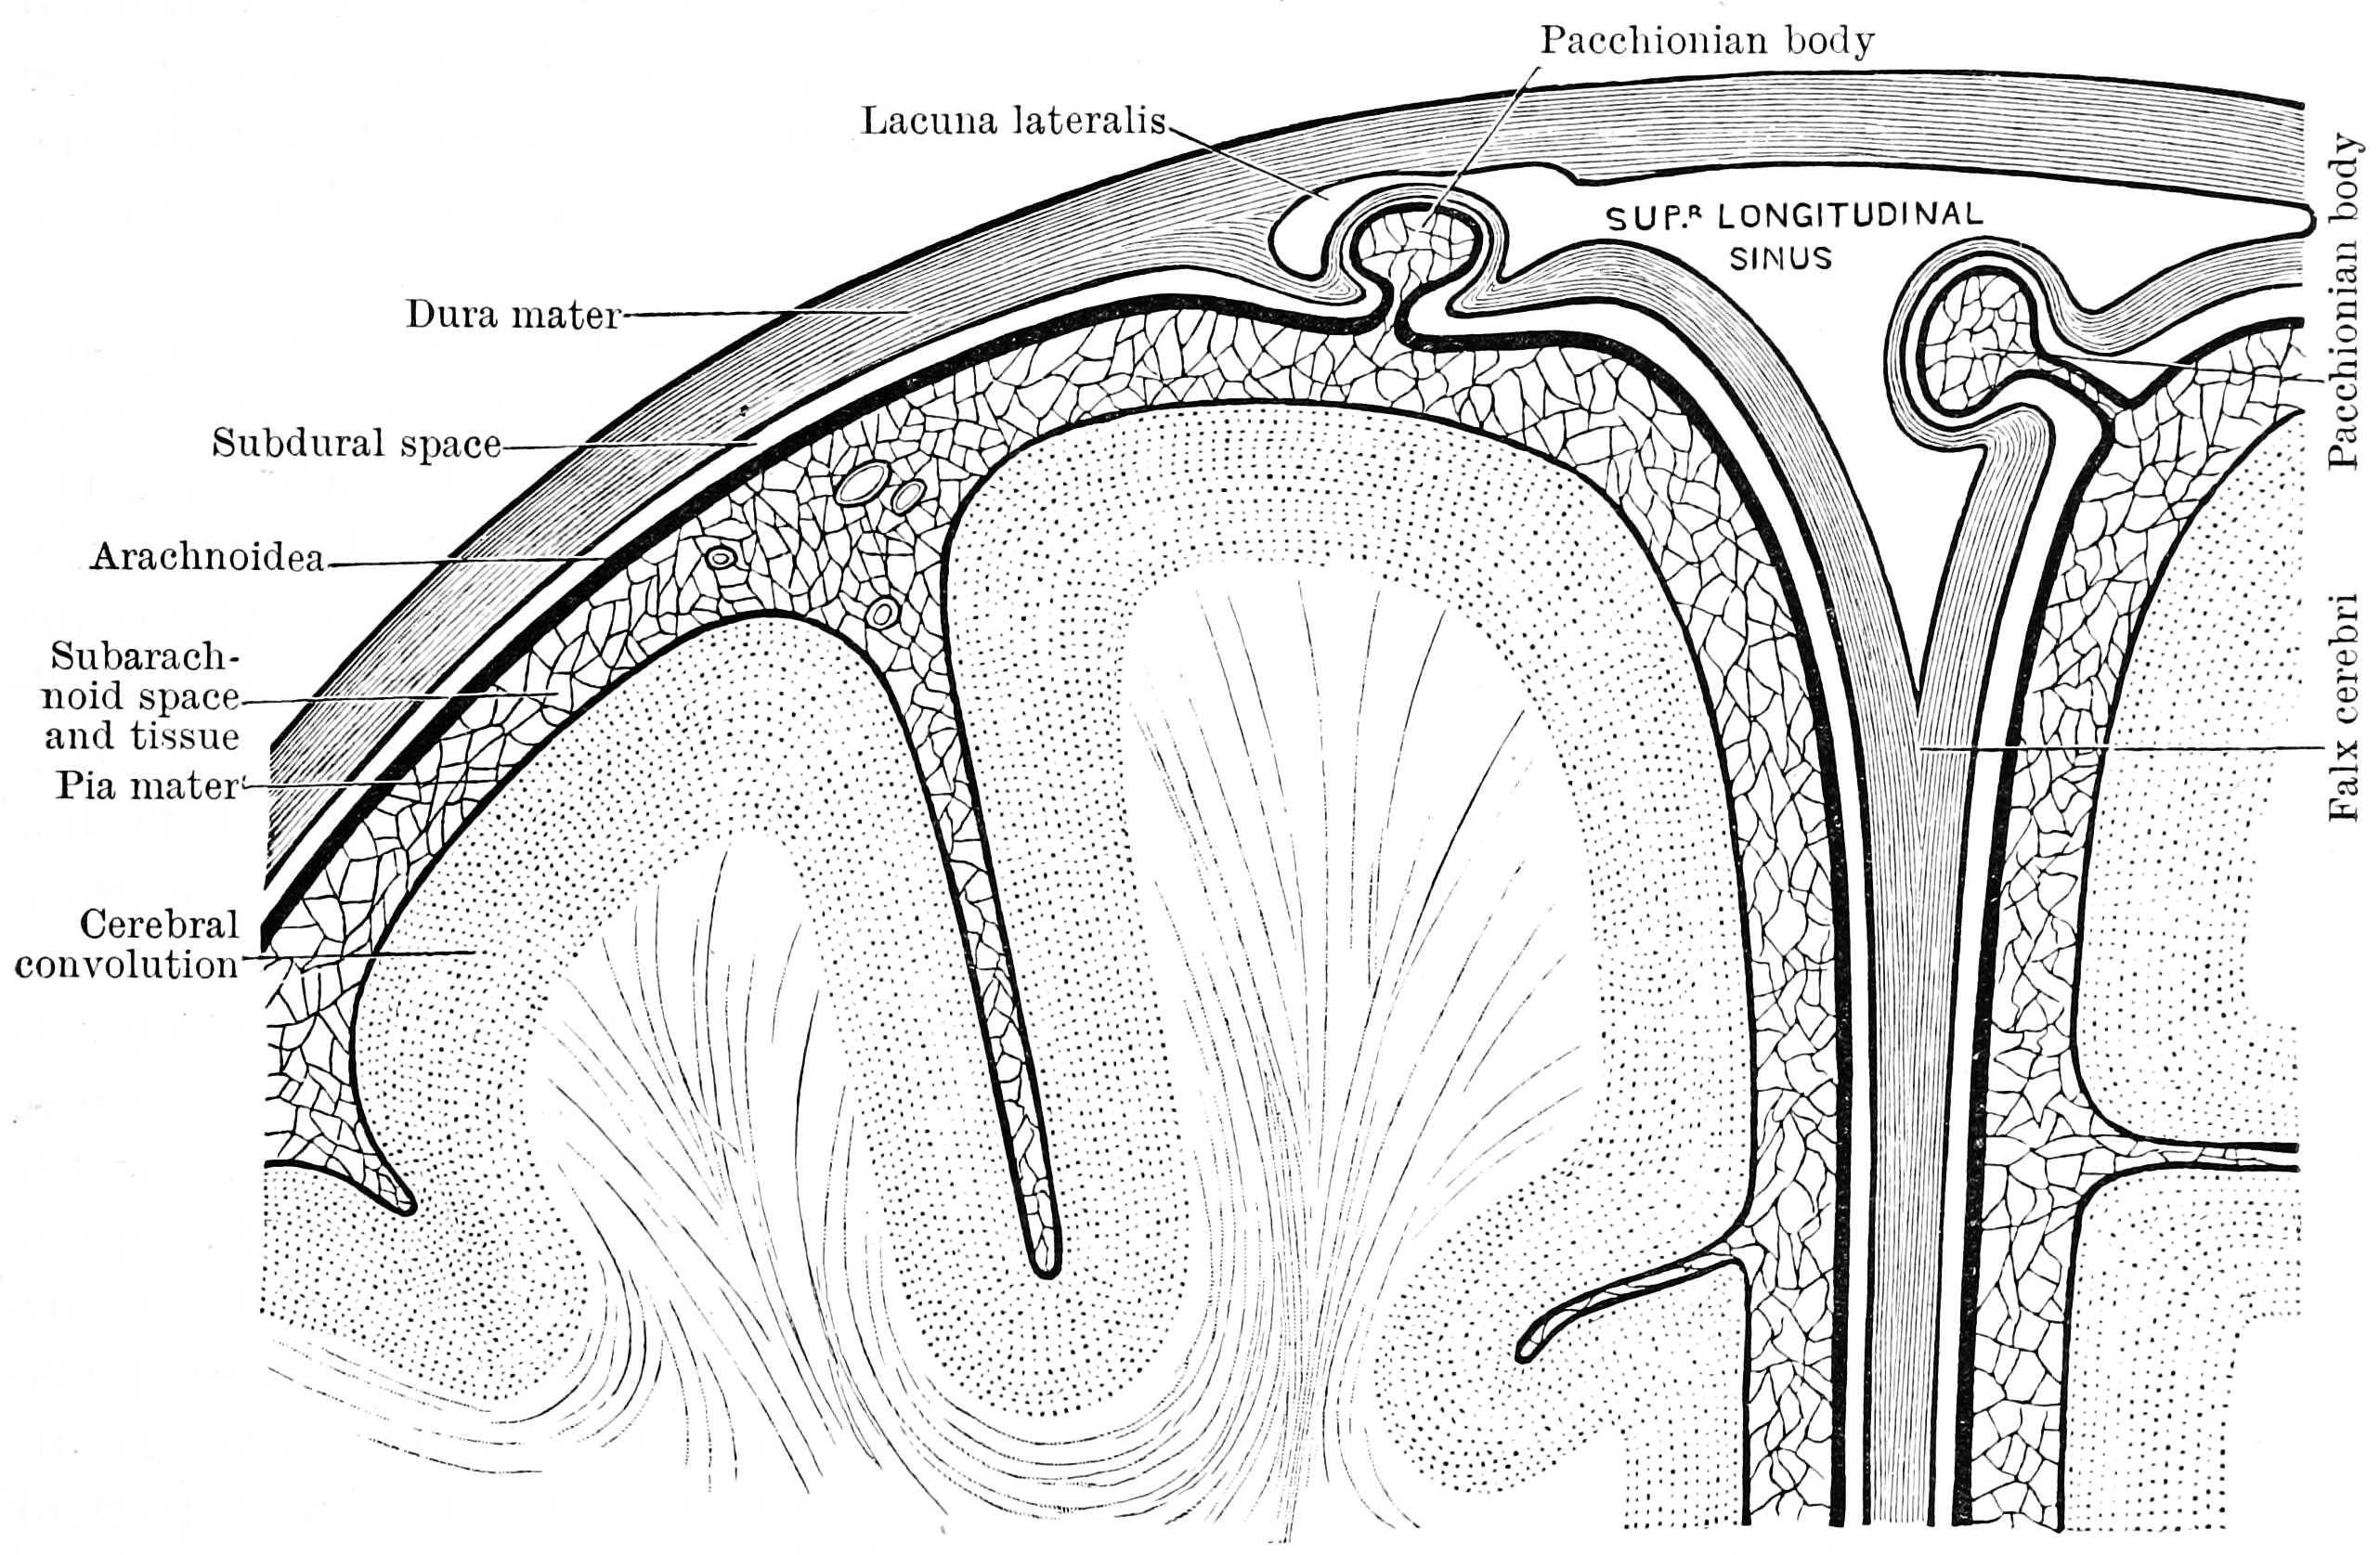
\includegraphics[width=0.7\linewidth]{./figures/cns/meninges} 

}

\caption{Diagram showing the relationship of the meninges to the skull and brain. \href{https://wellcomelibrary.org/item/b21271070}{Textbook of anatomy. Section 2. The muscular system: the nervous system: the organs of sense and integument edited by D. J. Cunningham}}\label{fig:meninges}
\end{figure}

\hypertarget{the-ventricular-system}{%
\section{The Ventricular System}\label{the-ventricular-system}}

The ventricular system is a set of four interconnected cavities (ventricles) in the brain, where the cerebrospinal fluid (CSF) is produced. Within each ventricle is a region of choroid plexus, a network of ependymal cells involved in the production of CSF. The ventricular system is continuous with the central canal of the spinal cord (from the fourth ventricle), allowing for the flow of CSF to circulate. All of the ventricular system and the central canal of the spinal cord are lined with ependyma, a specialised form of epithelium.



\begin{figure}

{\centering 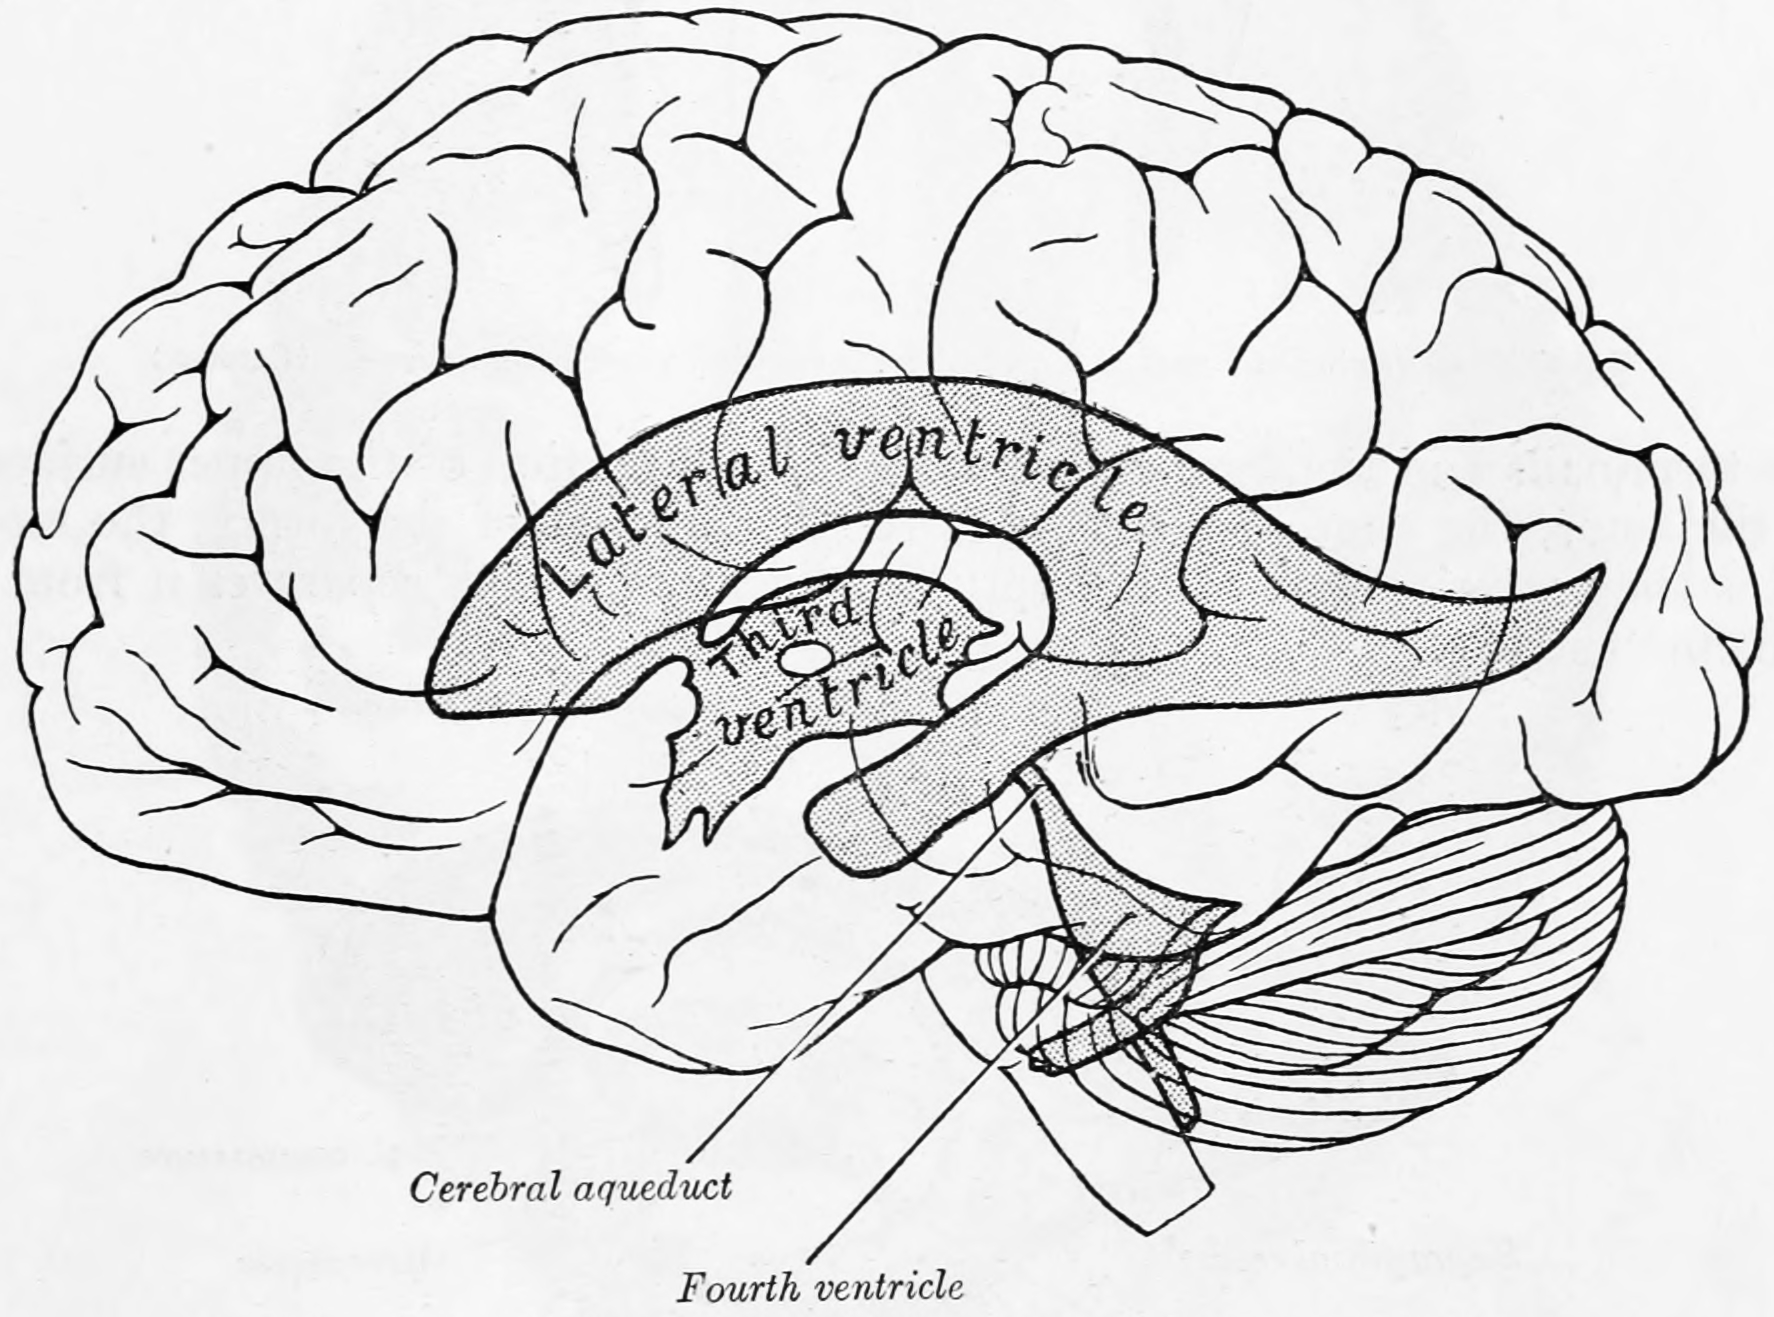
\includegraphics[width=0.7\linewidth]{./figures/cns/GrayAnat1918p829} 

}

\caption{The ventricles in relation to the brain as seen through the left hemisphere. From \href{https://archive.org/details/anatomyofhumanbo1918gray/page/n6/mode/2up}{Gray Henry, Anatomy of the Human Body. 20\textsuperscript{th} Edition, Lea \& Febiger, Philadelphia \& New York, 1918}}\label{fig:ventriclesbrain}
\end{figure}

The system comprises four ventricles:

\begin{itemize}
\tightlist
\item
  lateral ventricles right and left (one for each hemisphere)
\item
  third ventricle
\item
  fourth ventricle
\end{itemize}



\begin{figure}

{\centering 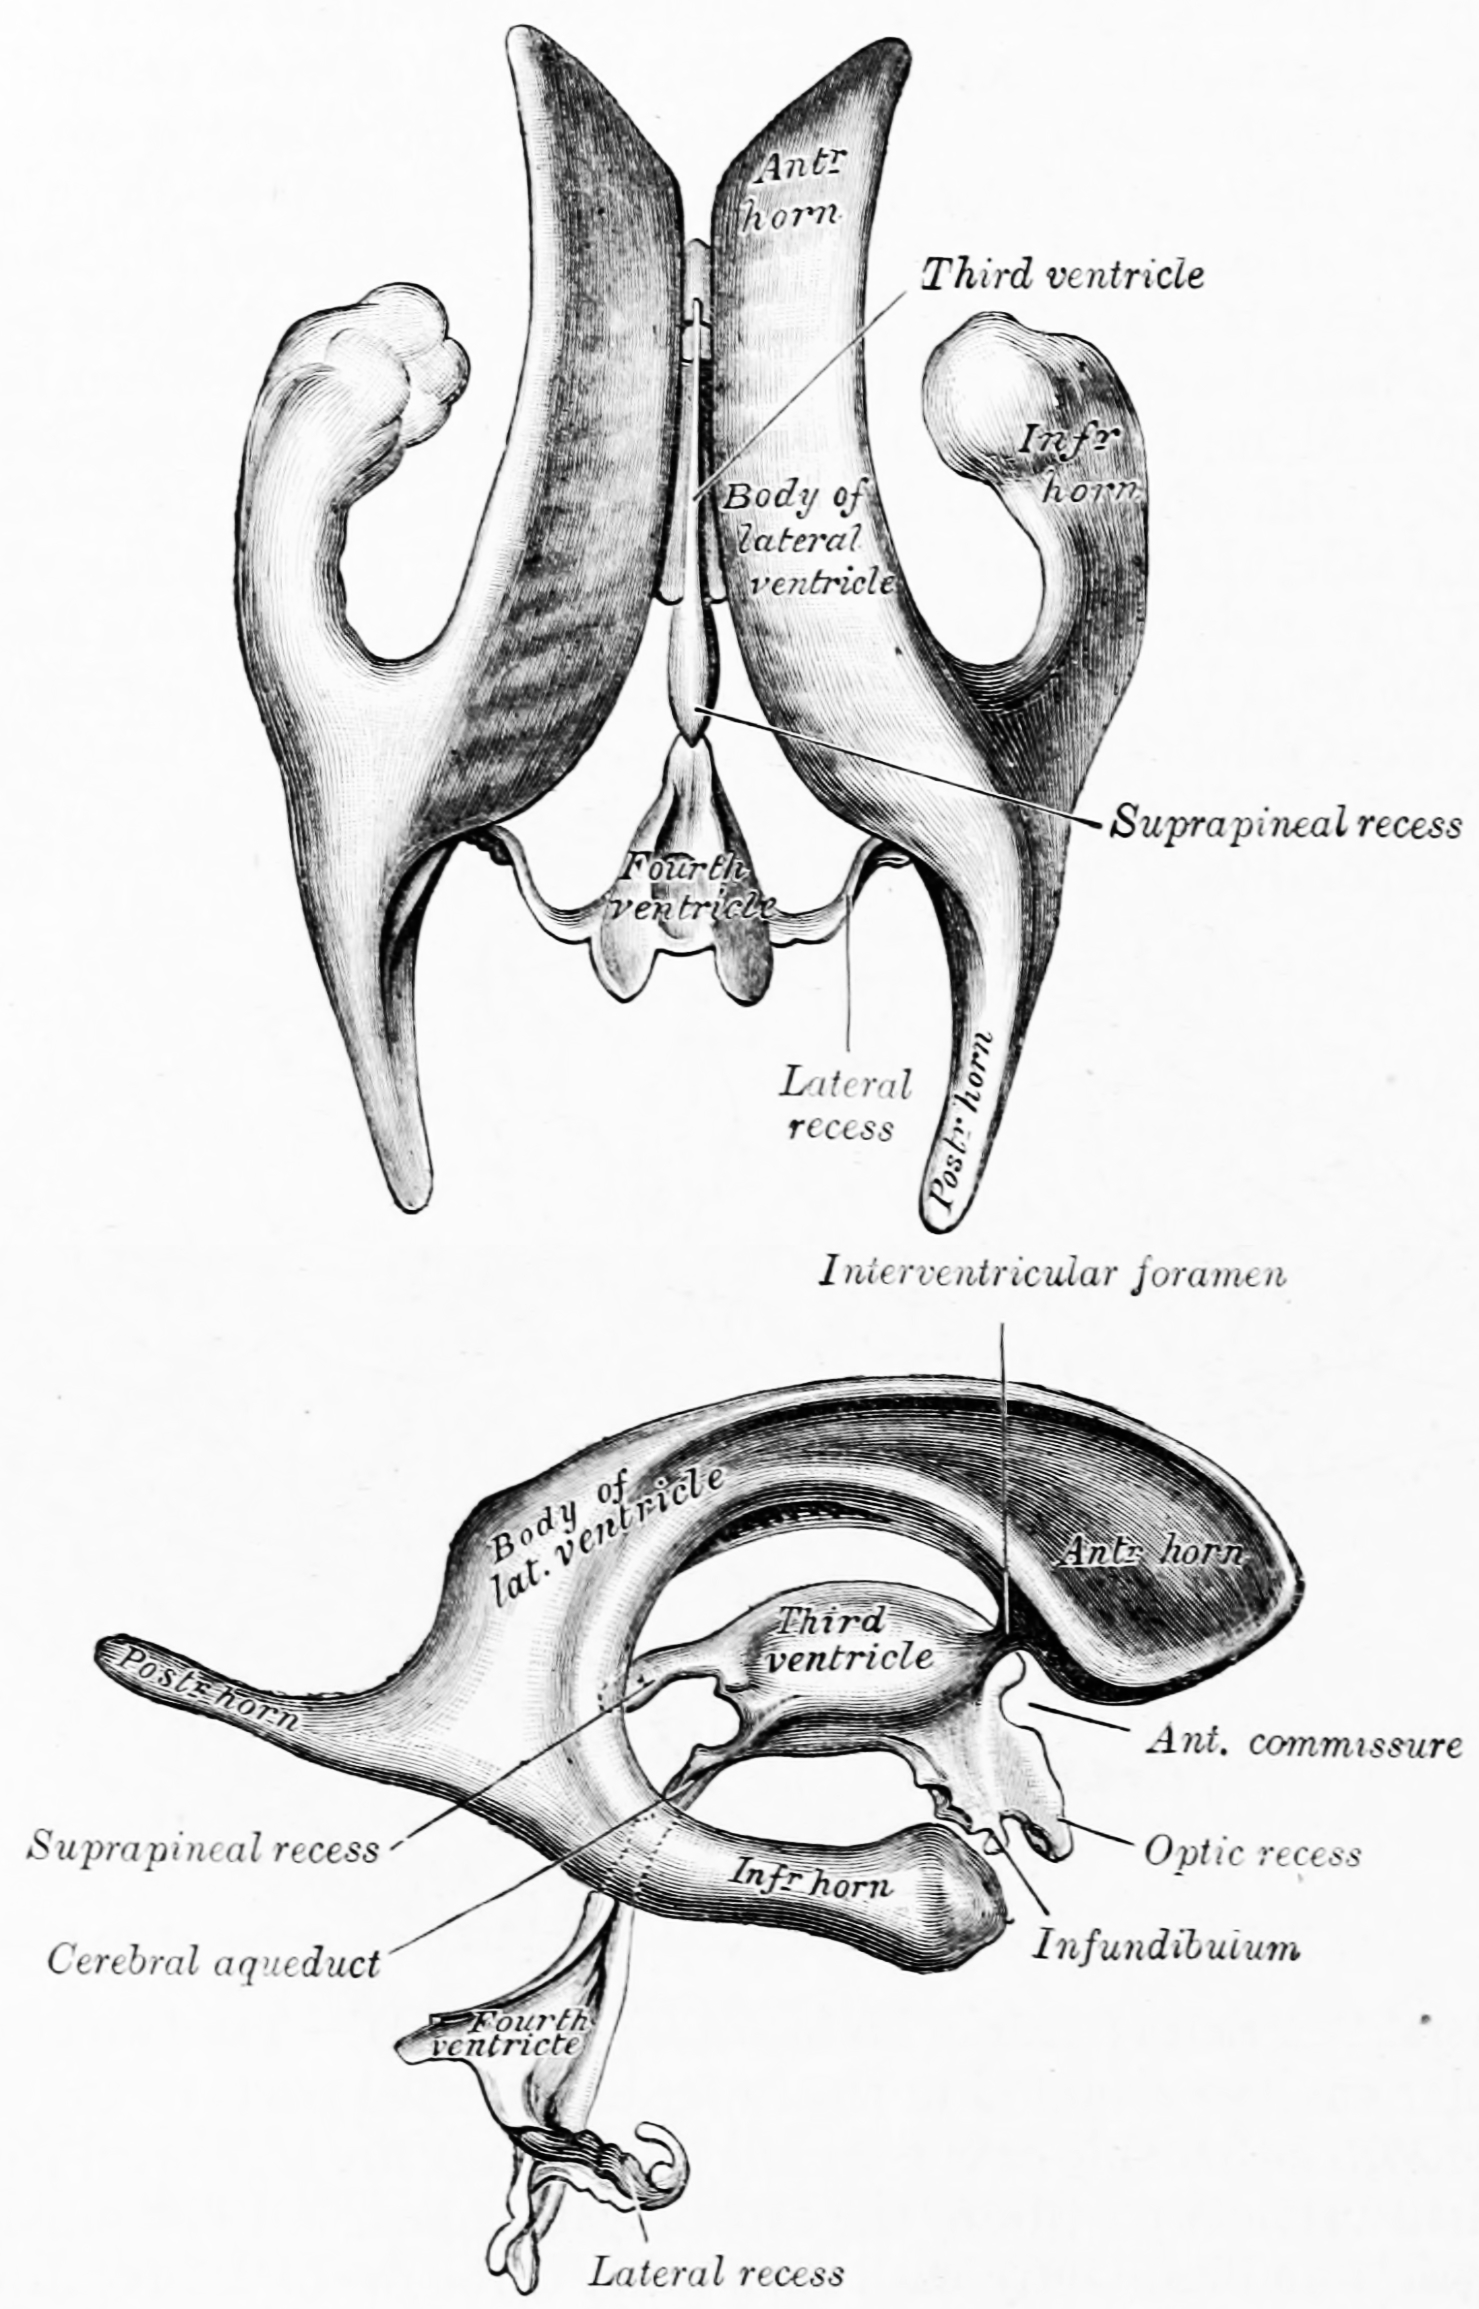
\includegraphics[width=0.7\linewidth]{./figures/cns/GrayAnat1918p830} 

}

\caption{The ventricular system of the brain as seen from above (top) and the side (bottom). From \href{https://archive.org/details/anatomyofhumanbo1918gray/page/n6/mode/2up}{Gray Henry, Anatomy of the Human Body. 20\textsuperscript{th} Edition, Lea \& Febiger, Philadelphia \& New York, 1918}}\label{fig:ventricles}
\end{figure}

There are several foramina, openings acting as channels, that connect the ventricles. The interventricular foramina (also called the foramina of Monro) connect the lateral ventricles to the third ventricle through which the cerebrospinal fluid can flow.

\begin{longtable}[]{@{}lll@{}}
\toprule
\begin{minipage}[b]{0.34\columnwidth}\raggedright
Name\strut
\end{minipage} & \begin{minipage}[b]{0.34\columnwidth}\raggedright
From\strut
\end{minipage} & \begin{minipage}[b]{0.23\columnwidth}\raggedright
To\strut
\end{minipage}\tabularnewline
\midrule
\endhead
\begin{minipage}[t]{0.34\columnwidth}\raggedright
interventricular foramina (Monro)\strut
\end{minipage} & \begin{minipage}[t]{0.34\columnwidth}\raggedright
lateral ventricles\strut
\end{minipage} & \begin{minipage}[t]{0.23\columnwidth}\raggedright
third ventricle\strut
\end{minipage}\tabularnewline
\begin{minipage}[t]{0.34\columnwidth}\raggedright
cerebral aqueduct (Sylvius)\strut
\end{minipage} & \begin{minipage}[t]{0.34\columnwidth}\raggedright
third ventricle\strut
\end{minipage} & \begin{minipage}[t]{0.23\columnwidth}\raggedright
fourth ventricle\strut
\end{minipage}\tabularnewline
\begin{minipage}[t]{0.34\columnwidth}\raggedright
median aperture (Magendie)\strut
\end{minipage} & \begin{minipage}[t]{0.34\columnwidth}\raggedright
fourth ventricle\strut
\end{minipage} & \begin{minipage}[t]{0.23\columnwidth}\raggedright
subarachnoid space via the cisterna magna\strut
\end{minipage}\tabularnewline
\begin{minipage}[t]{0.34\columnwidth}\raggedright
right and left lateral aperture (Luschka)\strut
\end{minipage} & \begin{minipage}[t]{0.34\columnwidth}\raggedright
fourth ventricle\strut
\end{minipage} & \begin{minipage}[t]{0.23\columnwidth}\raggedright
subarachnoid space via the cistern of great cerebral vein\strut
\end{minipage}\tabularnewline
\bottomrule
\end{longtable}

The ventricles are filled with cerebrospinal fluid (CSF) which bathes and cushions the brain and spinal cord within their bony confines. CSF is produced by modified ependymal cells of the choroid plexus found in all components of the ventricular system except for the cerebral aqueduct and the posterior and anterior horns of the lateral ventricles. CSF flows from the lateral ventricles via the interventricular foramina into the third ventricle, and then the fourth ventricle via the cerebral aqueduct in the brainstem. From the fourth ventricle it can pass into the central canal of the spinal cord or into the subarachnoid cisterns via three small foramina: the central median aperture and the two lateral apertures.

The fluid then flows around the superior sagittal sinus to be reabsorbed via the arachnoid granulations (or arachnoid villi) into the venous sinuses, after which it passes through the jugular vein and major venous system. CSF within the spinal cord can flow all the way down to the lumbar cistern at the end of the cord around the cauda equina where lumbar punctures are performed.

The cerebral aqueduct between the third and fourth ventricles is very small, as are the foramina, which means that they can be easily blocked.

\hypertarget{the-cerebrospinal-fluid}{%
\section{The Cerebrospinal Fluid}\label{the-cerebrospinal-fluid}}

Cerebrospinal fluid (CSF) is a clear, colorless body fluid found in the brain and spinal cord. It is produced by specialised ependymal cells in the choroid plexuses of the ventricles of the brain, and absorbed in the arachnoid granulations. There is about 125mL of CSF at any one time, and about 500 mL is generated every day. CSF acts as a cushion or buffer, providing basic mechanical and immunological protection to the brain inside the skull. CSF also serves a vital function in the cerebral autoregulation of cerebral blood flow.

CSF occupies the subarachnoid space (between the arachnoid mater and the pia mater) and the ventricular system around and inside the brain and spinal cord. It fills the ventricles of the brain, cisterns, and sulci, as well as the central canal of the spinal cord. There is also a connection from the subarachnoid space to the bony labyrinth of the inner ear via the perilymphatic duct where the perilymph is continuous with the cerebrospinal fluid. The ependymal cells of the choroid plexuses have multiple motile cilia on their apical surfaces that beat to move the CSF through the ventricles.

A sample of CSF can be taken via lumbar puncture. This can reveal the intracranial pressure, as well as indicate diseases including infections of the brain or its surrounding meninges. Although noted by Hippocrates, it was only in the 18th century that \href{https://en.wikipedia.org/wiki/Emanuel_Swedenborg}{Emanuel Swedenborg} was credited with its rediscovery, and as late as 1914 \href{https://en.wikipedia.org/wiki/Harvey_Cushing}{Harvey Cushing} demonstrated CSF was secreted by the choroid plexus.

\hypertarget{the-blood-brain-barrier}{%
\section{The Blood-Brain-Barrier}\label{the-blood-brain-barrier}}

The blood--brain barrier (BBB) is a highly selective semipermeable border that separates the circulating blood from the brain and extracellular fluid in the central nervous system (CNS). The blood-brain barrier is formed by endothelial cells of the capillary wall, astrocyte end-feet (also known as ``glia limitans'') ensheathing the capillary, and pericytes embedded in the capillary basement membrane. This system allows the passage of some molecules by passive diffusion, as well as the selective transport of molecules such as glucose, water and amino acids that are crucial to neural function.

Specialized structures participating in sensory and secretory integration within neural circuits---the circumventricular organs and choroid plexus---do not have a blood-brain barrier.

The blood-brain barrier restricts the passage of pathogens, the diffusion of solutes in the blood, and large or hydrophilic molecules into the cerebrospinal fluid (CSF), while allowing the diffusion of hydrophobic molecules (O\textsubscript{2}, CO\textsubscript{2}, hormones) and small polar molecules. Cells of the barrier actively transport metabolic products such as glucose across the barrier using specific transport proteins.

Technically, the BBB is a shorthand for the Blood-CNS barrier, which has two parts: the Blood-Brain portion and the Blood-Spinal Cord Barrier portion. The two parts are often breached simultaneously, but may be independently breached.

The blood-brain barrier results from the selectivity of the tight junctions between endothelial cells in CNS vessels, which restricts the passage of solutes. At the interface between blood and the brain, endothelial cells are stitched together by these tight junctions, which are composed of smaller subunits, frequently biochemical dimers, that are transmembrane proteins such as occludin, claudins, junctional adhesion molecule (JAM), or ESAM, for example. Each of these transmembrane proteins is anchored into the endothelial cells by another protein complex that includes ZO-1 and associated proteins.

Several areas of the human brain are not on the brain side of the BBB. Some examples of this include the circumventricular organs, the roof of the third and fourth ventricles, capillaries in the pineal gland on the roof of the diencephalon and the pineal gland. The pineal gland secretes the hormone melatonin ``directly into the systemic circulation'', thus melatonin is not affected by the blood-brain barrier.

The blood-brain barrier acts effectively to protect the brain from circulating pathogens. Accordingly, blood-borne infections of the brain are rare. Infections of the brain that do occur are often difficult to treat. Antibodies are too large to cross the blood-brain barrier, and only certain antibiotics are able to pass. In some cases, a drug has to be administered directly into the cerebrospinal fluid (CSF) where it can enter the brain by crossing the blood-cerebrospinal fluid barrier.

The blood-brain barrier may become leaky in select neurological diseases, such as amyotrophic lateral sclerosis, epilepsy, brain trauma and edema, and in systemic diseases, such as liver failure. The blood-brain barrier becomes more permeable during inflammation, allowing antibiotics and phagocytes to move across the BBB. However, this also allows bacteria and viruses to infiltrate the blood-brain barrier. Examples of pathogens that can traverse the blood-brain barrier include \emph{Toxoplasma gondii} which causes toxoplasmosis, spirochetes like \emph{Borrelia} (Lyme disease), Group B streptococci which causes meningitis in newborns, and \emph{Treponema pallidum} which causes syphilis. Some of these harmful bacteria gain access by releasing cytotoxins like pneumolysin which have a direct toxic effect on brain microvascular endothelium and tight junctions.



\begin{figure}

{\centering 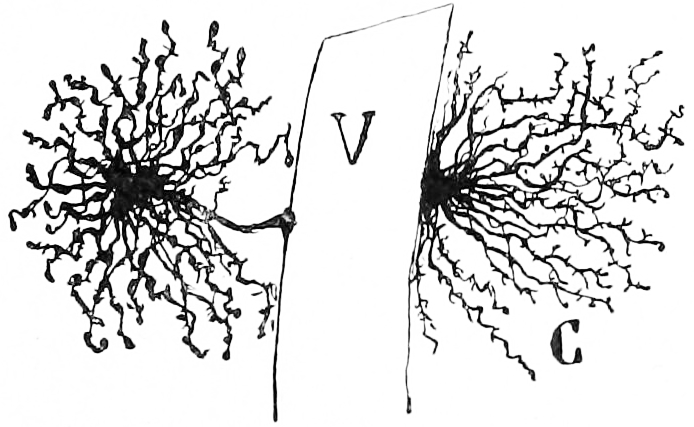
\includegraphics[width=0.7\linewidth]{./figures/cns/astrocytes_vessel} 

}

\caption{Astrocytes in the grey matter of the cerebral cortex with their endfeet on brain capillaries. \href{https://wellcomelibrary.org/item/b2129592x\#?c=0\&m=0\&s=0\&cv=14\&z=0\%2C-3.48\%2C1\%2C8.6591}{Histologie du système nerveux de l'homme \& des vertébrés, Tome Premier} (1909) by Santiago Ramón y Cajal translated from Spanish by Dr.~L. Azoulay.}\label{fig:astrobbb}
\end{figure}



\begin{figure}

{\centering 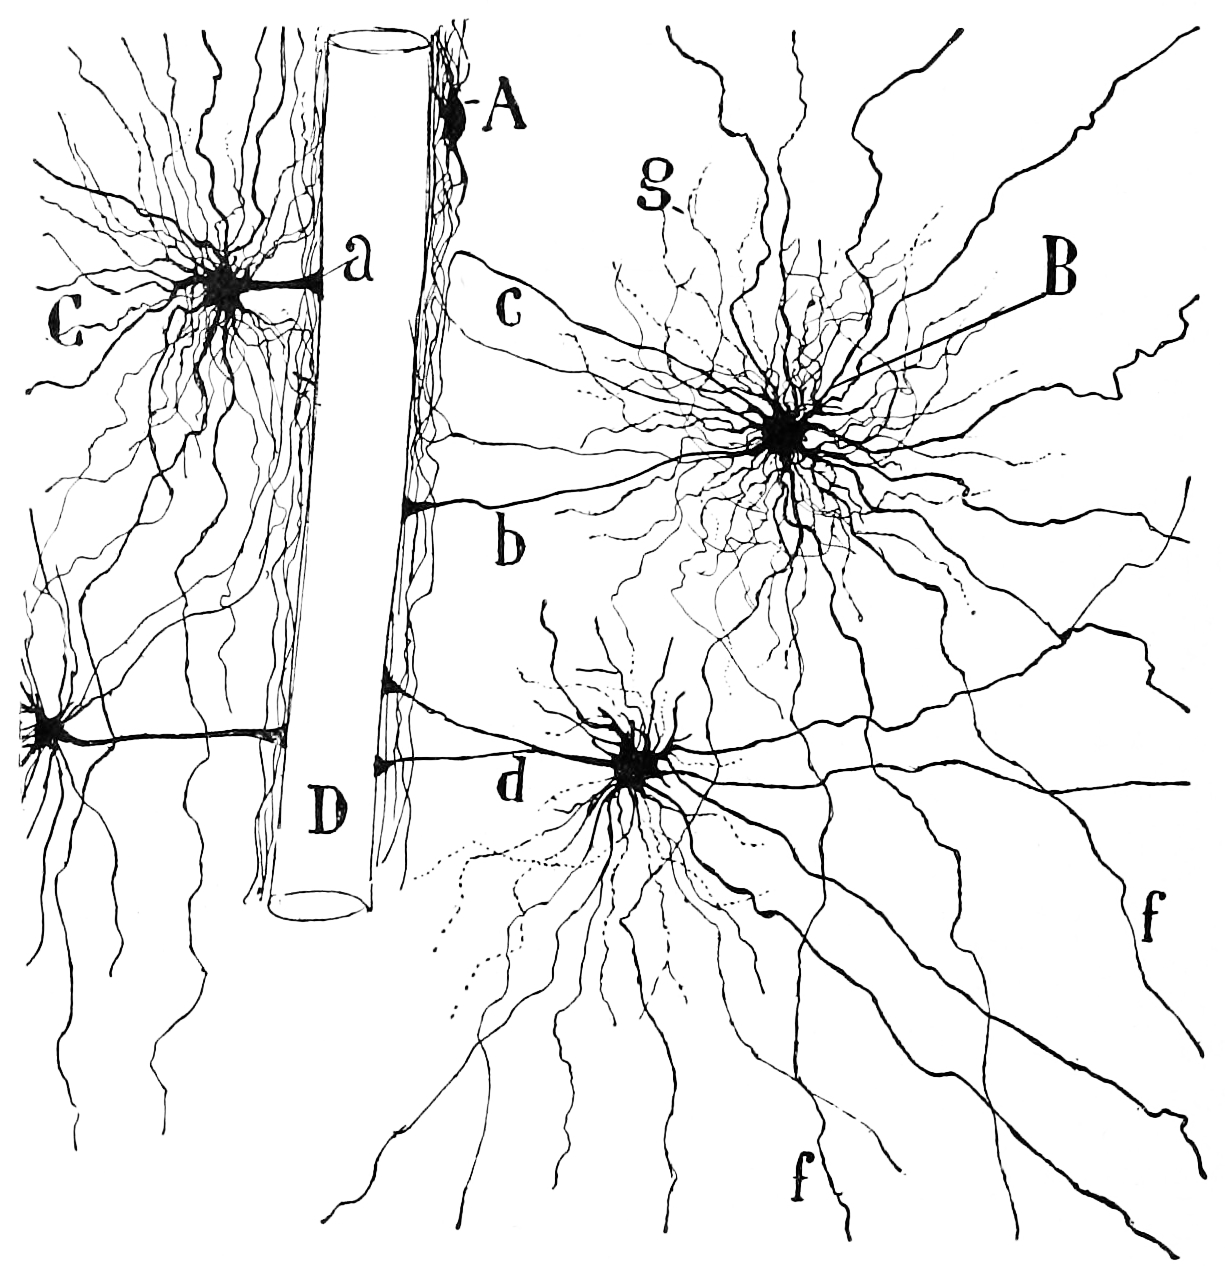
\includegraphics[width=0.7\linewidth]{./figures/cns/ologodendrocytes_vessel} 

}

\caption{Oligodendrocytes in the white matter of the cerebral cortex with their endfeet touching a brain capillary. \href{https://wellcomelibrary.org/item/b2129592x\#?c=0\&m=0\&s=0\&cv=14\&z=0\%2C-3.48\%2C1\%2C8.6591}{Histologie du système nerveux de l'homme \& des vertébrés, Tome Premier} (1909) by Santiago Ramón y Cajal translated from Spanish by Dr.~L. Azoulay.}\label{fig:oligobbb}
\end{figure}

\hypertarget{circumventricular-organs}{%
\subsection{Circumventricular Organs}\label{circumventricular-organs}}

Circumventricular organs (CVOs) are individual structures located adjacent to the fourth ventricle or third ventricle in the brain, and are characterized by dense capillary beds with permeable endothelial cells unlike those of the blood-brain barrier. Included among CVOs having highly permeable capillaries are the area postrema, subfornical organ, vascular organ of the lamina terminalis, median eminence, pineal gland, and three lobes of the pituitary gland.

Permeable capillaries of the sensory CVOs (area postrema, subfornical organ, vascular organ of the lamina terminalis) enable rapid detection of circulating signals in systemic blood, while those of the secretory CVOs (median eminence, pineal gland, pituitary lobes) facilitate transport of brain-derived signals into the circulating blood. Consequently, the CVO permeable capillaries are the point of bidirectional blood-brain communication for neuroendocrine function.

The border zones between brain tissue ``behind'' the blood-brain barrier and zones ``open'' to blood signals in certain CVOs contain specialized hybrid capillaries that are leakier than typical brain capillaries, but not as permeable as CVO capillaries. Such zones exist at the border of the area postrema---nucleus tractus solitarii (NTS), and median eminence---hypothalamic arcuate nucleus.

\href{https://en.wikipedia.org/wiki/Paul_Ehrlich}{Paul Ehrlich} was a bacteriologist studying staining, a procedure that is used in many microscopy studies to make fine biological structures visible using chemical dyes. As Ehrlich injected some of these dyes (notably the aniline dyes that were then widely used), the dye stained all of the organs of some kinds of animals except for their brains. At that time, Ehrlich attributed this lack of staining to the brain simply not picking up as much of the dye.

However, in a later experiment in 1913, \href{https://en.wikipedia.org/wiki/Edwin_Goldmann}{Edwin Goldmann} (one of Ehrlich's students) injected the dye directly into the cerebrospinal fluids of animal brains. He found then the brains did become dyed, but the rest of the body did not, demonstrating the existence of a compartmentalization between the two. At that time, it was thought that the blood vessels themselves were responsible for the barrier, since no obvious membrane could be found. The term blood--brain barrier was coined in 1900 by the German neurologist \href{https://en.wikipedia.org/wiki/Max_Lewandowsky}{Max Lewandowsky}.

\hypertarget{the-cerebrum}{%
\section{The Cerebrum}\label{the-cerebrum}}

The cerebrum is the largest part of the brain, and is divided into nearly symmetrical left and right hemispheres by a deep groove, the longitudinal fissure (Figure \ref{fig:topview}). The hemispheres are connected by five commissures that span the longitudinal fissure, the largest of these is the corpus callosum (Figure \ref{fig:medialview}). Each hemisphere is conventionally divided into four main lobes; the frontal lobe, parietal lobe, temporal lobe, and occipital lobe, named according to the skull bones that overlie them. The surface of the brain is folded into ridges (gyri) and grooves (sulci), many of which are named, usually according to their position, such as the frontal gyrus of the frontal lobe or the central sulcus separating the central regions of the hemispheres. There are many small variations in the secondary and tertiary folds.



\begin{figure}

{\centering 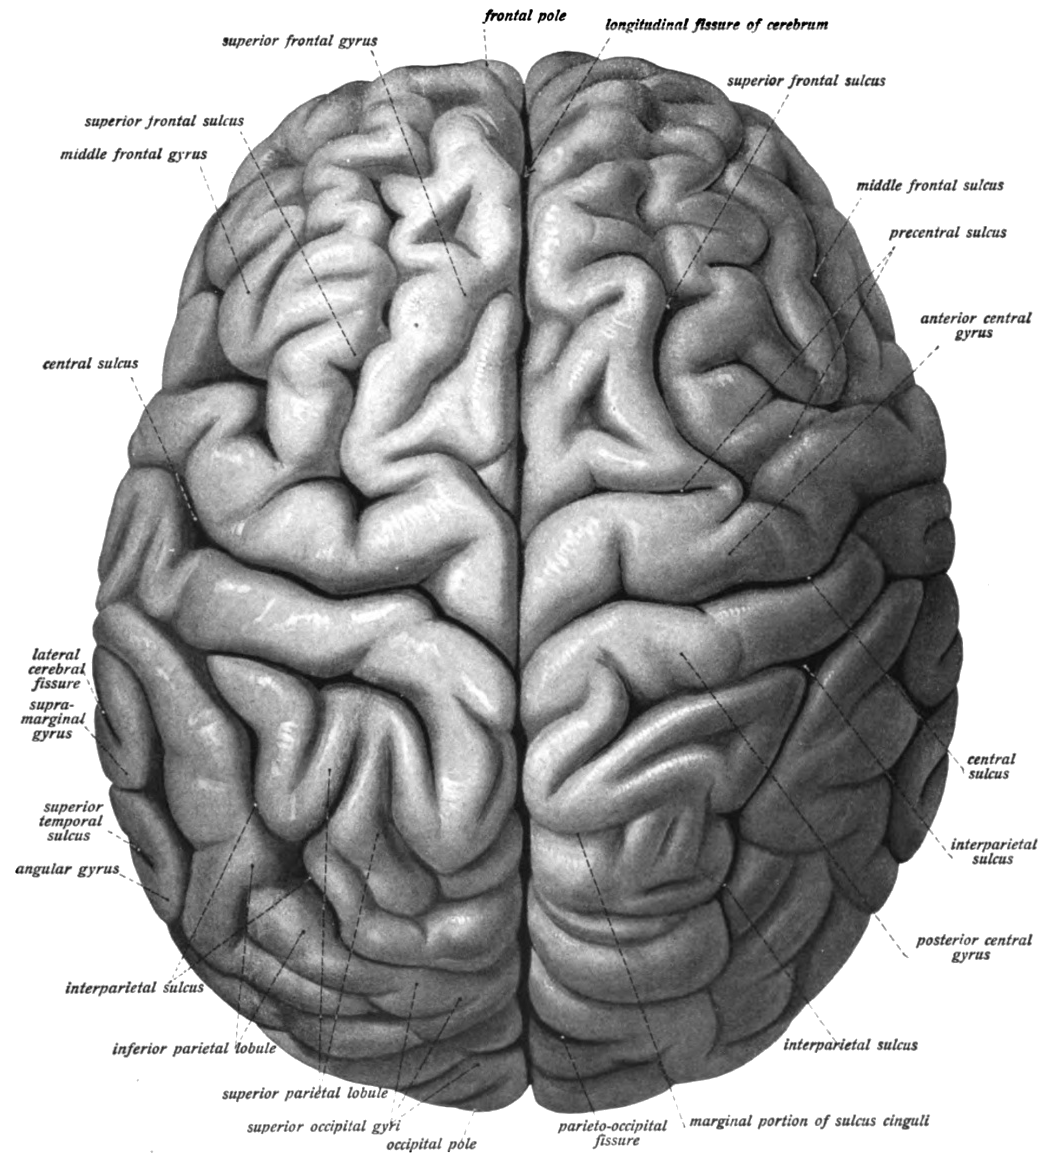
\includegraphics[width=0.7\linewidth]{./figures/cns/Sobo_1909_628} 

}

\caption{View of the human brain (cerebrum) showing the left and right hemispheres from the top. \href{https://commons.wikimedia.org/wiki/File:Sobo_1909_628.png}{Sobotta's Textbook and Atlas of Human Anatomy 1909}}\label{fig:topview}
\end{figure}



\begin{figure}

{\centering 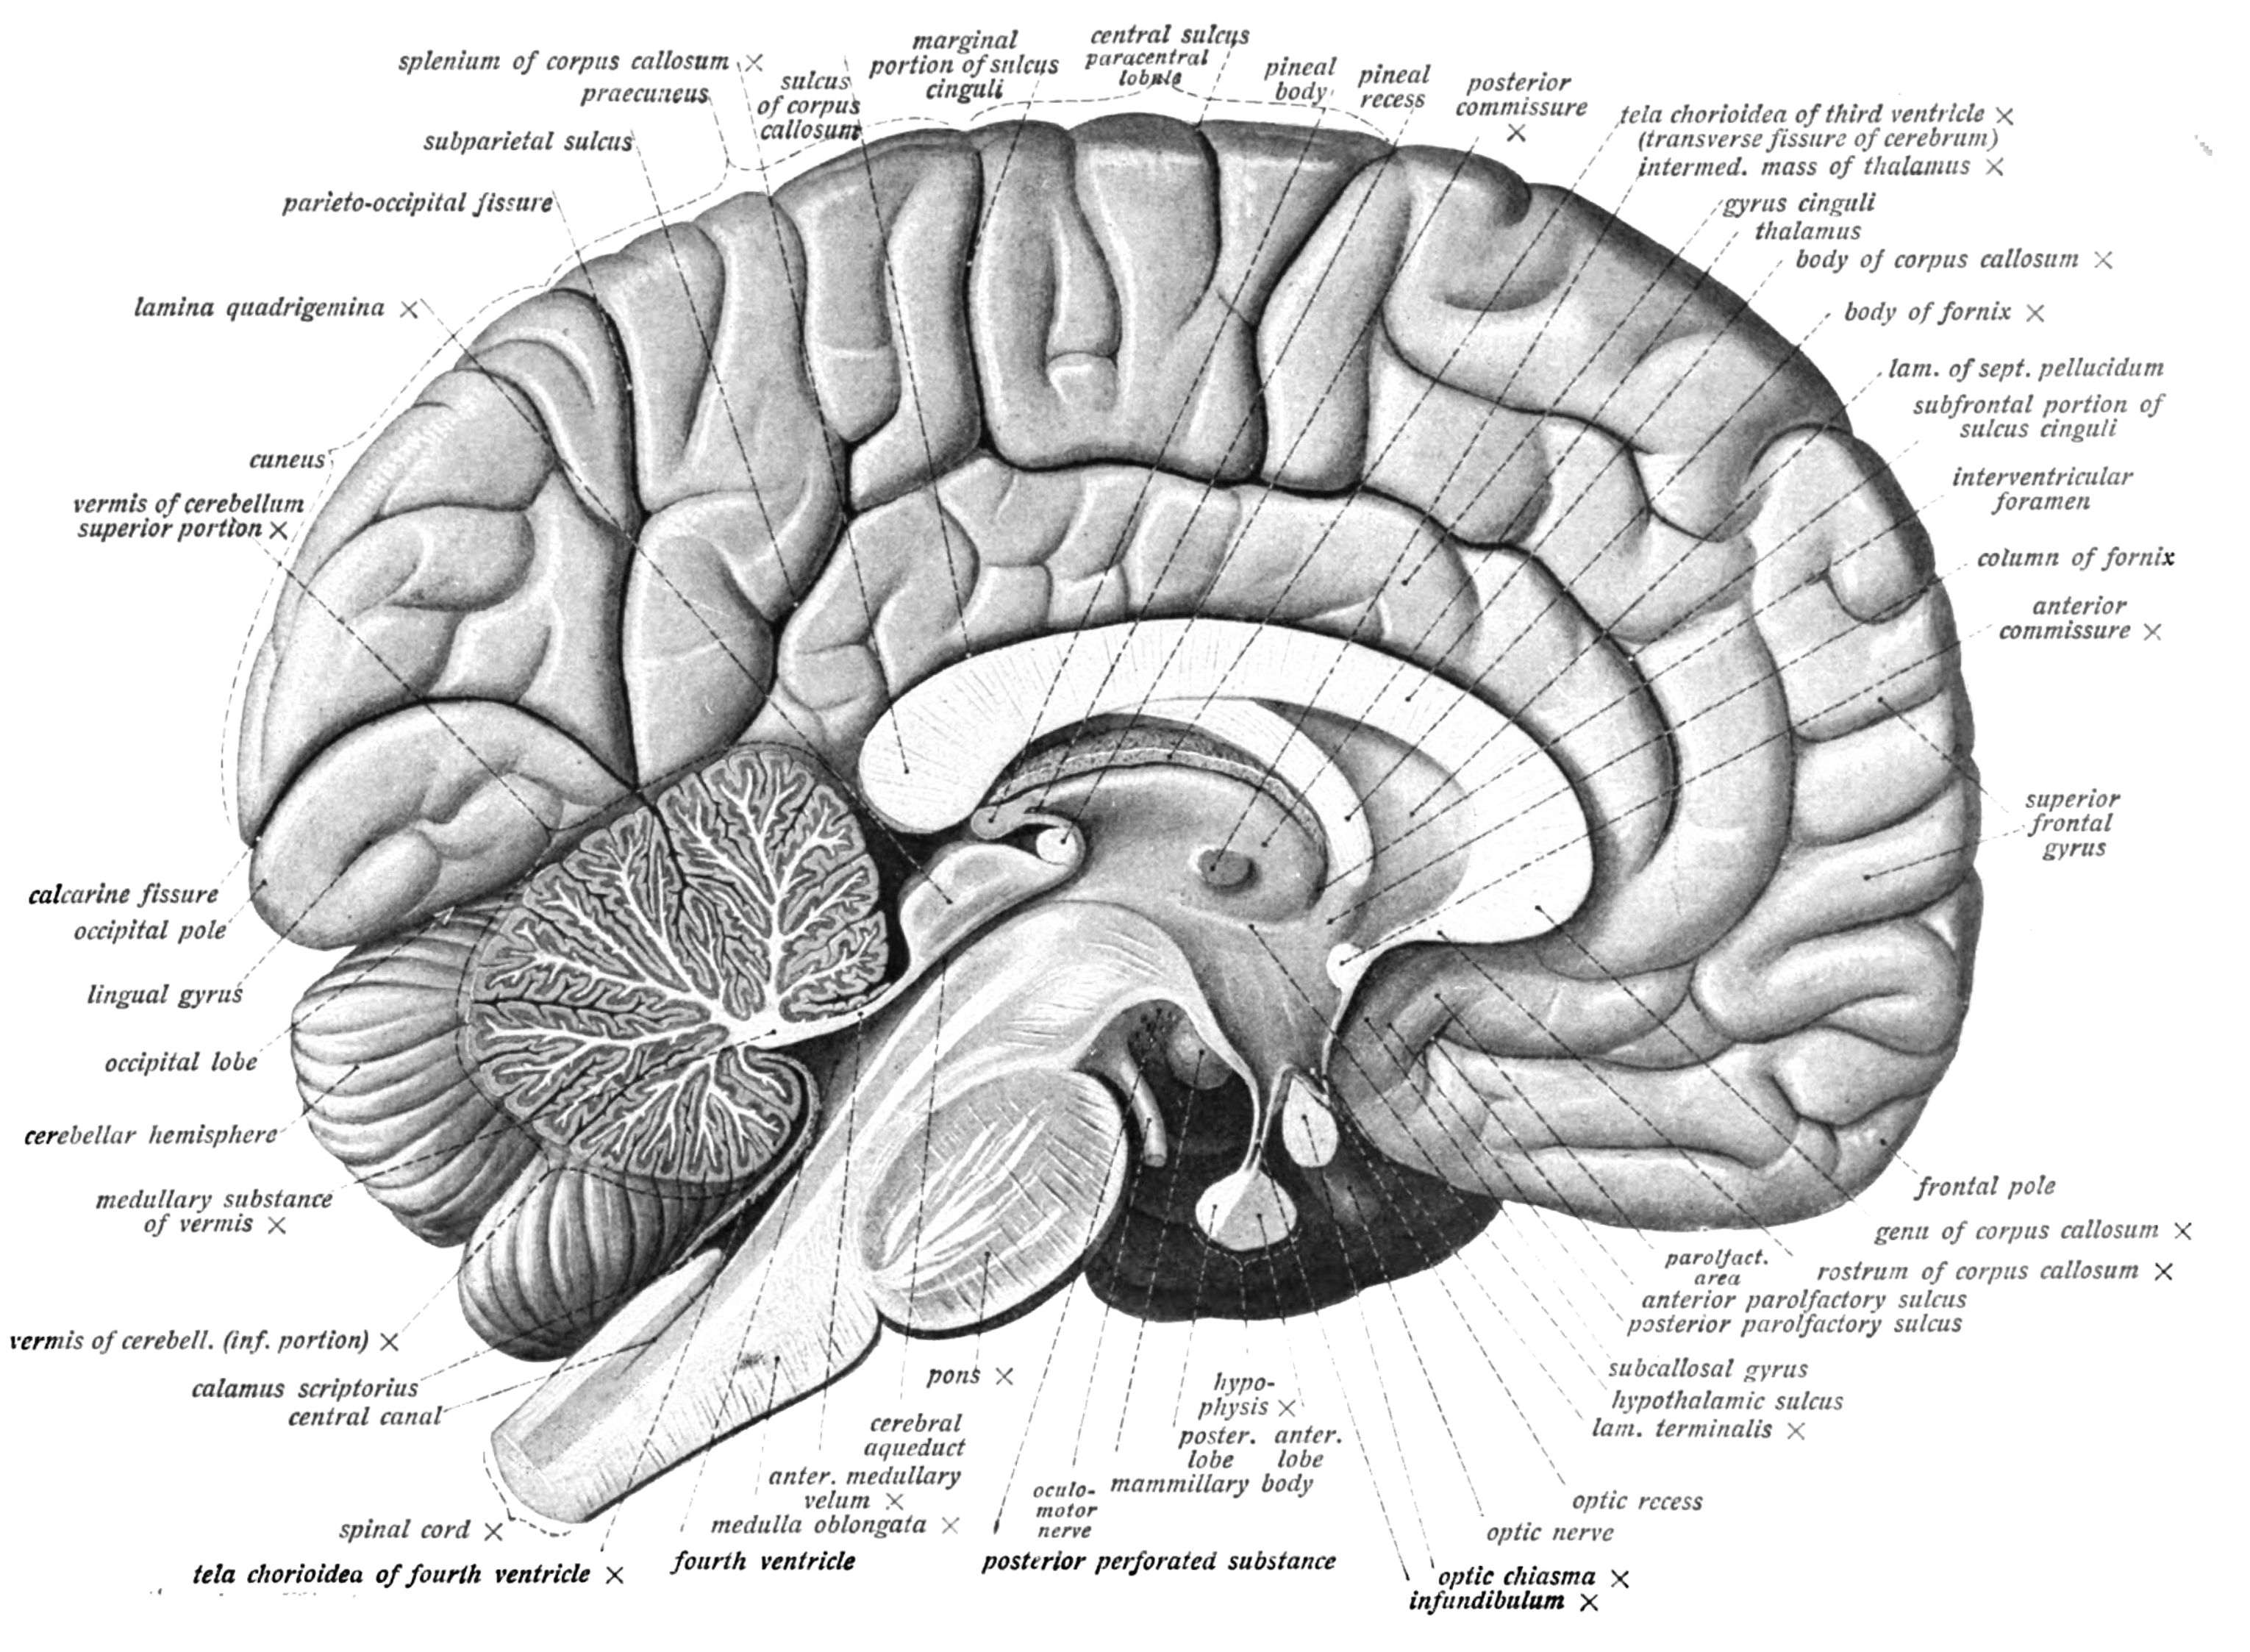
\includegraphics[width=0.7\linewidth]{./figures/cns/Sobo_1909_624} 

}

\caption{Medial view of the left hemisphere of the human brain. \href{https://commons.wikimedia.org/wiki/File:Sobo_1909_624.png}{Sobotta's Textbook and Atlas of Human Anatomy 1909}}\label{fig:medialview}
\end{figure}



\begin{figure}

{\centering 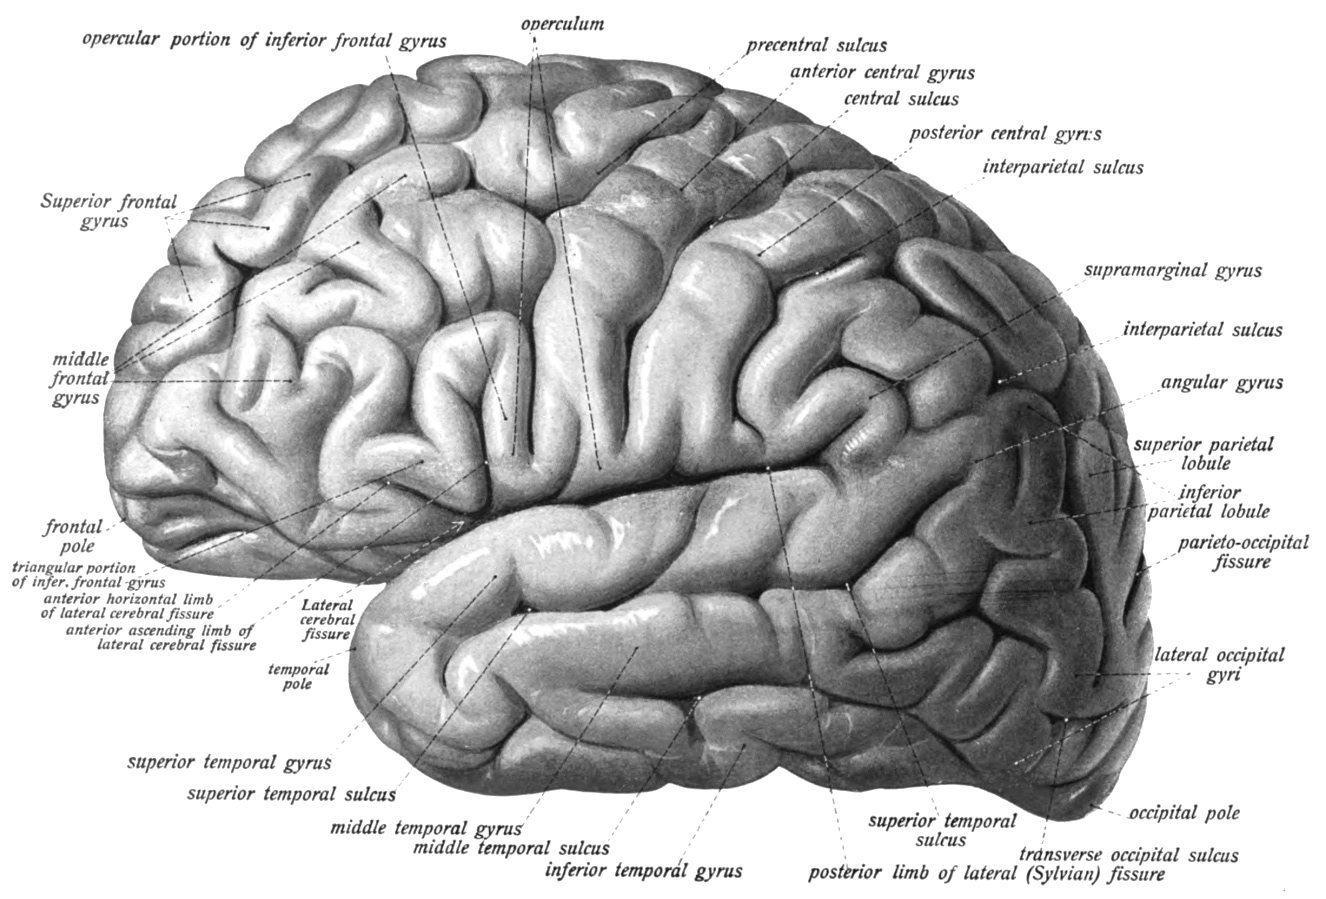
\includegraphics[width=0.7\linewidth]{./figures/cns/Sobo_1909_626} 

}

\caption{Lateral view of the left hemisphere of the human brain. \href{https://commons.wikimedia.org/wiki/File:Sobo_1909_626.png}{Sobotta's Textbook and Atlas of Human Anatomy 1909}}\label{fig:lateralview}
\end{figure}



\begin{figure}

{\centering 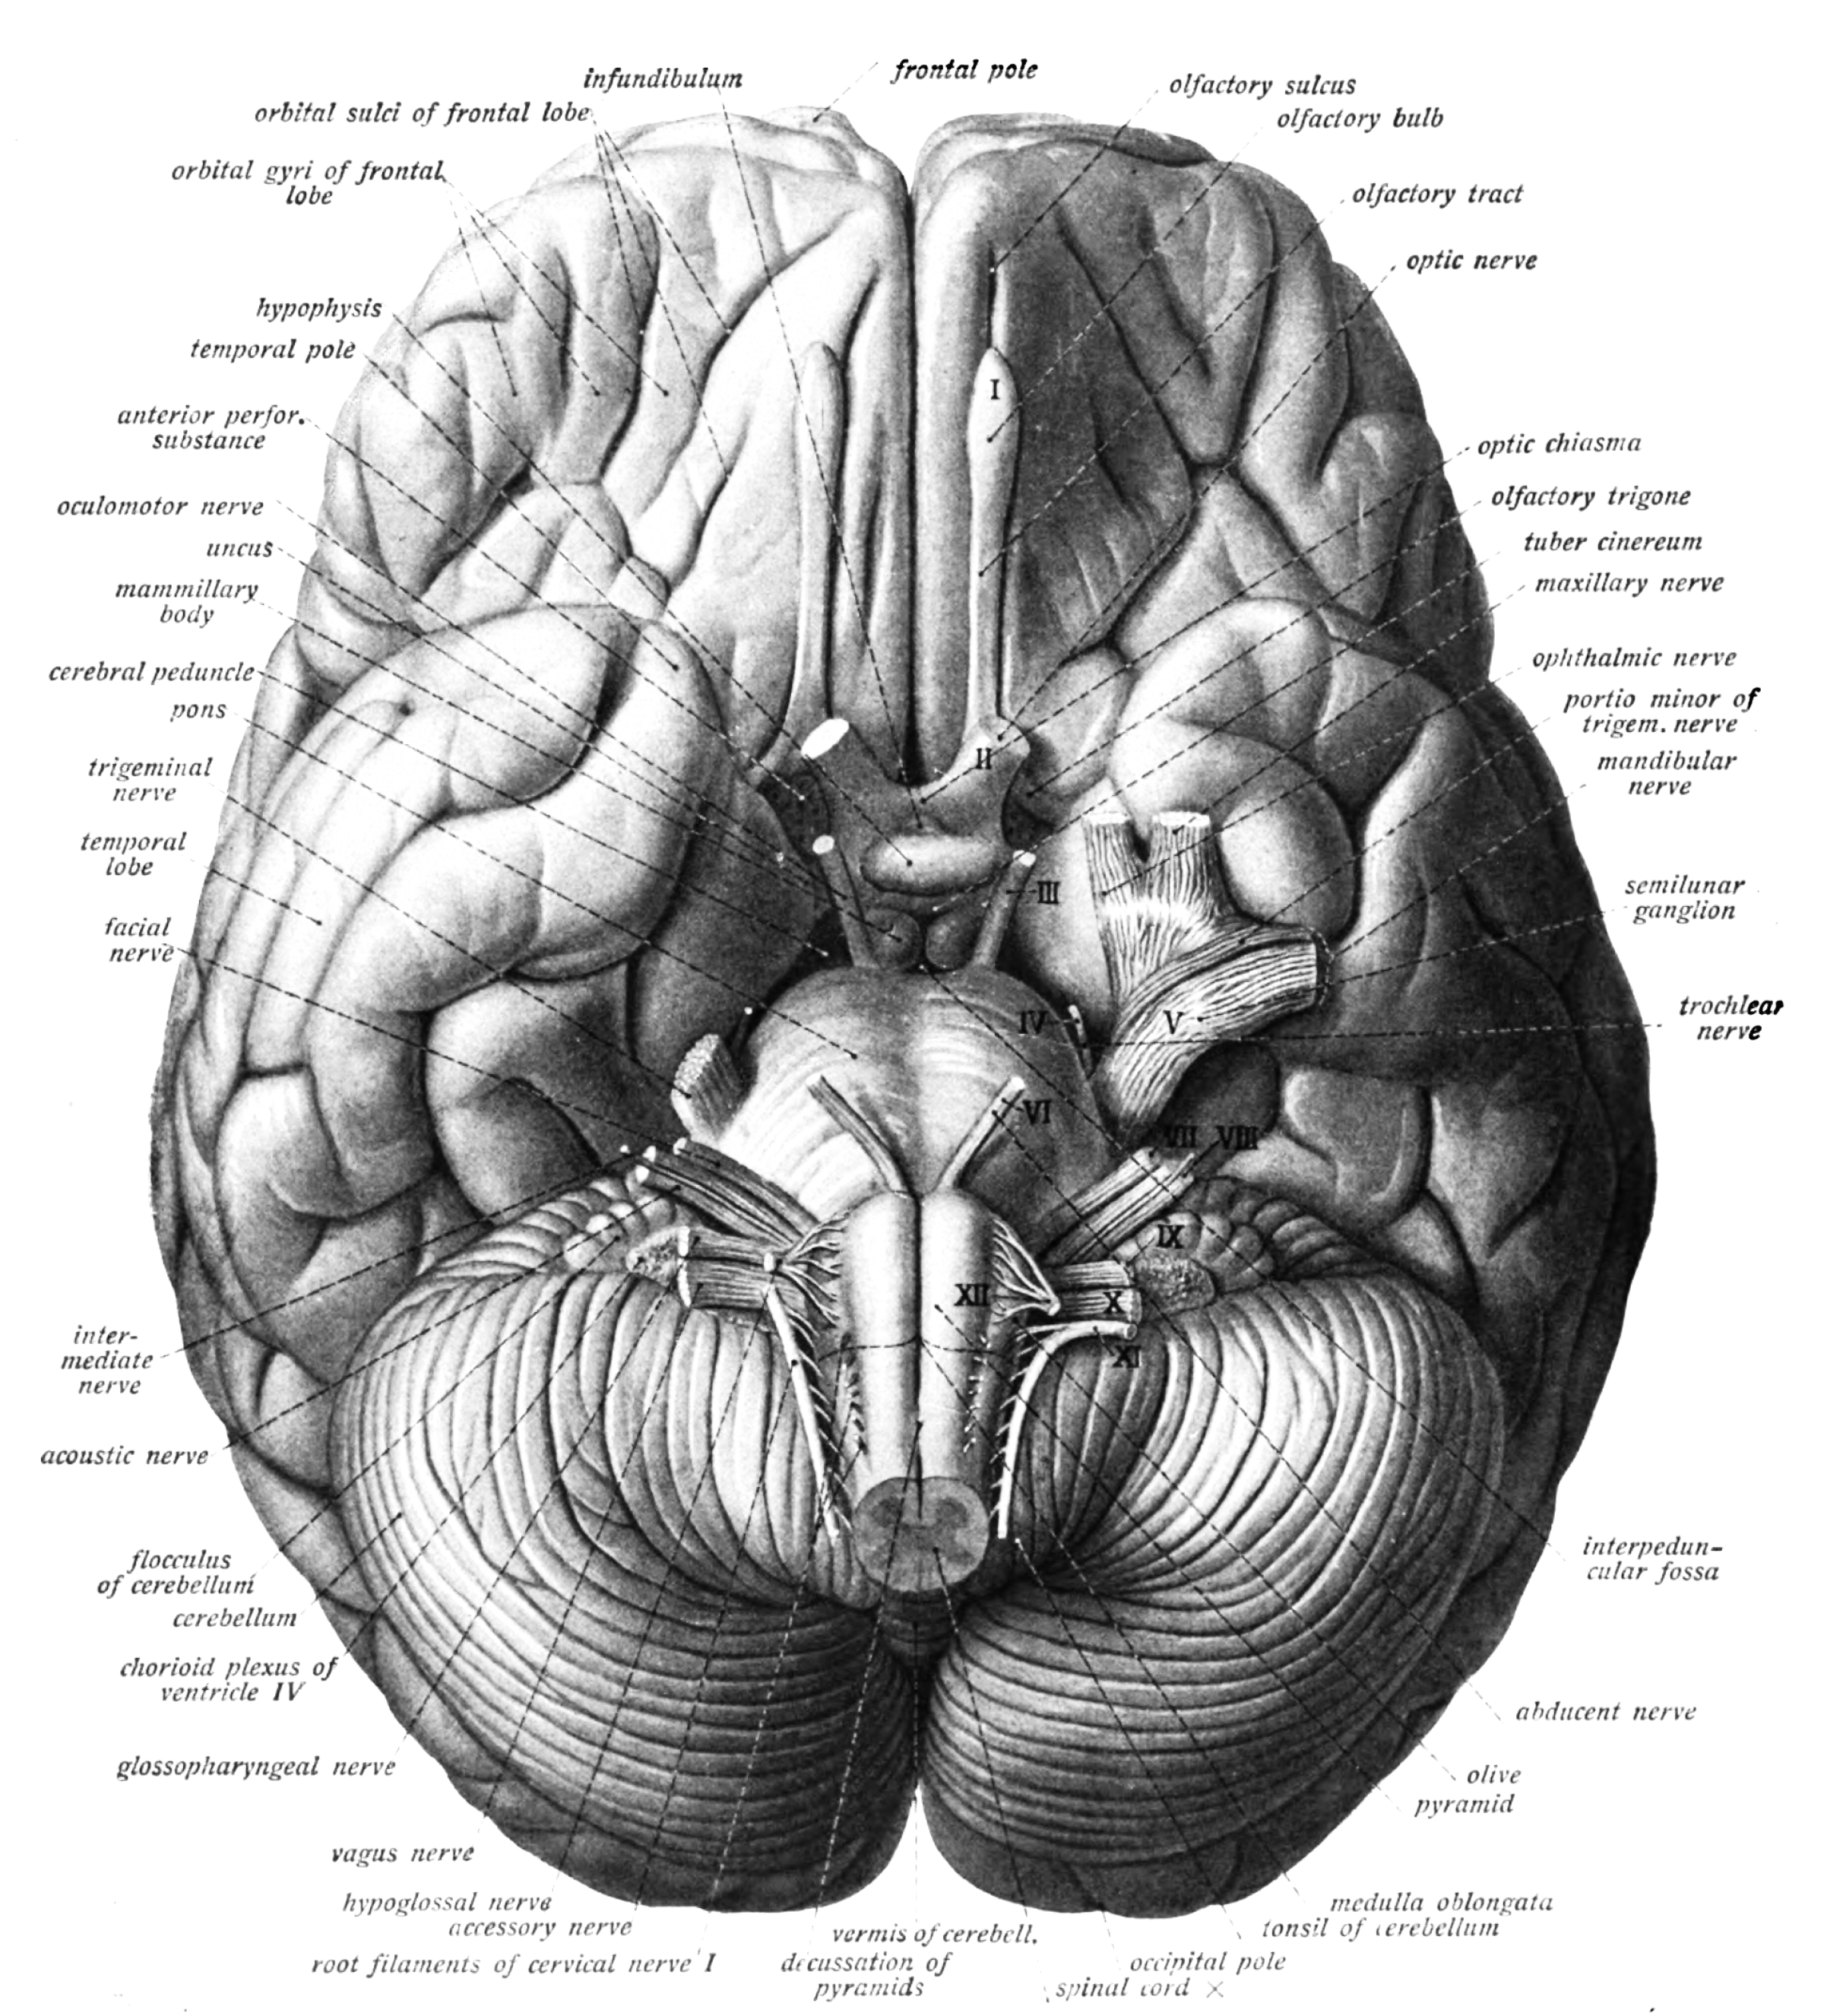
\includegraphics[width=0.7\linewidth]{./figures/cns/Sobo_1909_623} 

}

\caption{Bottom view of the human brain. \href{https://commons.wikimedia.org/wiki/File:Sobo_1909_623.png}{Sobotta's Textbook and Atlas of Human Anatomy 1909}}\label{fig:bottomview}
\end{figure}

\hypertarget{the-cerebral-cortex}{%
\subsection{The Cerebral Cortex}\label{the-cerebral-cortex}}

The outer part of the cerebrum is the cerebral cortex, made up of grey matter arranged in layers. It is 2 to 4 millimetres thick, and deeply folded to give a convoluted appearance. Beneath the cortex is the cerebral white matter (Figure \ref{fig:coronalsection}). Based on the differences in laminar organization the cerebral cortex can be classified into two types, the large area of neocortex which has six cell layers, and the much smaller area of allocortex that has three or four layers:



\begin{figure}

{\centering 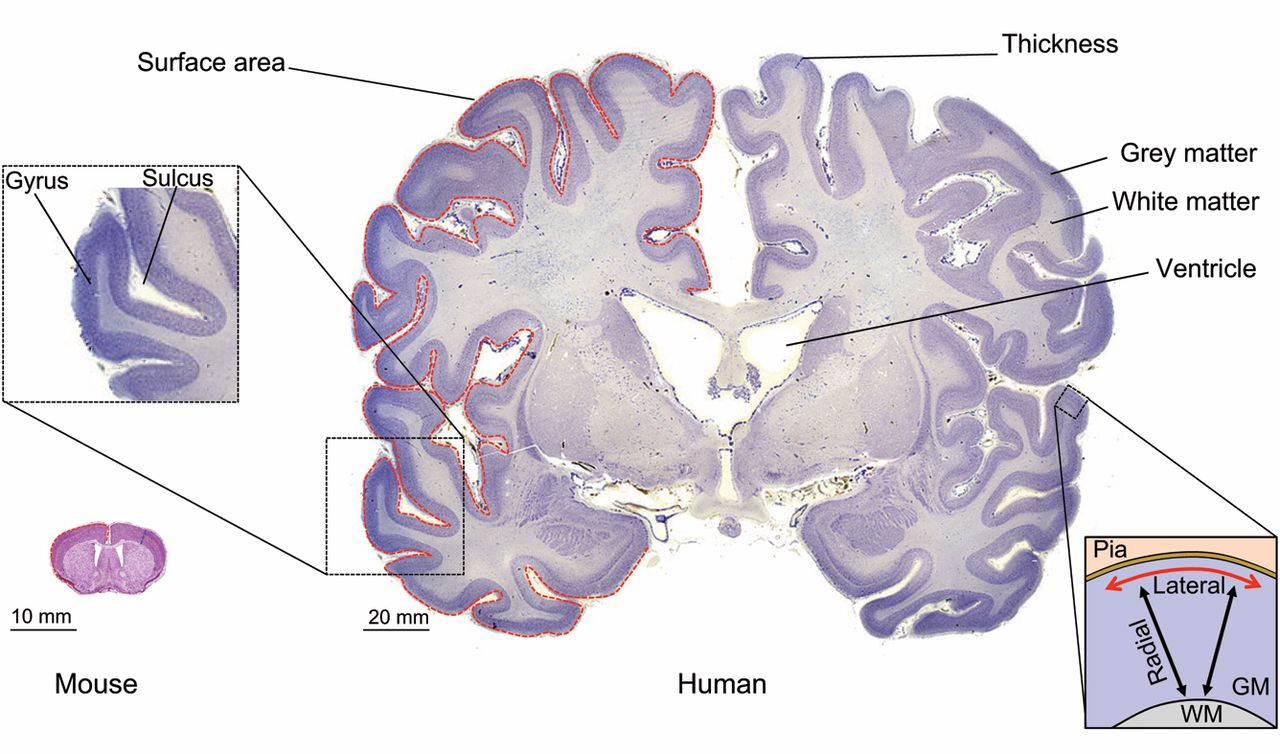
\includegraphics[width=0.7\linewidth]{./figures/cns/cortex_morphology} 

}

\caption{Neocortex morphology. Coronal sections of the mouse (left) and human (right) adult neocortex are shown. Red dashed lines highlight the contour of the pial surface of the gray matter (GM). Blue dashed lines highlight neocortical thickness. The inset on the left shows an area of the human neocortex at higher magnification, highlighting a neocortical gyrus that is contiguous to a sulcus. The inset on the right outlines the principal dimensions by which the adult neocortical GM is described: (1) radial (black arrows), i.e.~along the white matter (WM)-to-pia axis, corresponding to the apical-basal axis in terms of tissue polarity; and (2) lateral (red arrow), i.e.~along the axis perpendicular to the radial axis. Mouse neocortex adapted with permission from the High Resolution Mouse Brain Atlas (Sidman, R. L., Kosaras, B., Misra, B. M. and Senft, S. L., 1999), \url{http://www.hms.harvard.edu/research/brain}; human neocortex adapted with permission from \url{http://www.brains.rad.msu.edu} and \url{http://brainmuseum.org} (supported by the US National Science Foundation). From \href{https://dev.biologists.org/content/141/11/2182}{Marta Florio, Wieland B. Huttner(2014) Neural progenitors, neurogenesis and the evolution of the neocortex Development 2014 141: 2182-2194; doi: 10.1242/dev.090571}}\label{fig:cortexmorphology}
\end{figure}

\begin{itemize}
\tightlist
\item
  The neocortex is also known as the isocortex or neopallium and is the part of the mature cerebral cortex with six distinct layers. Examples of neocortical areas include the granular primary motor cortex, and the striate primary visual cortex (Figure \ref{fig:viscortex})". The neocortex has two subtypes, the true isocortex and the proisocortex which is a transitional region between the isocortex and the regions of the periallocortex.
\item
  The allocortex is the part of the cerebral cortex with three or four layers, and has three subtypes, the paleocortex with three cortical laminae, the archicortex which has four or five, and a transitional area adjacent to the allocortex, the periallocortex. Examples of allocortex are the olfactory cortex and the hippocampus.
\end{itemize}

Staining cross-sections of the cortex to reveal the position of neuronal cell bodies allowed neuroanatomists to produce a detailed description of the laminar structure of the cortex (Figure \ref{fig:cajallayers} and Figure \ref{fig:brodmannlayers}).



\begin{figure}

{\centering 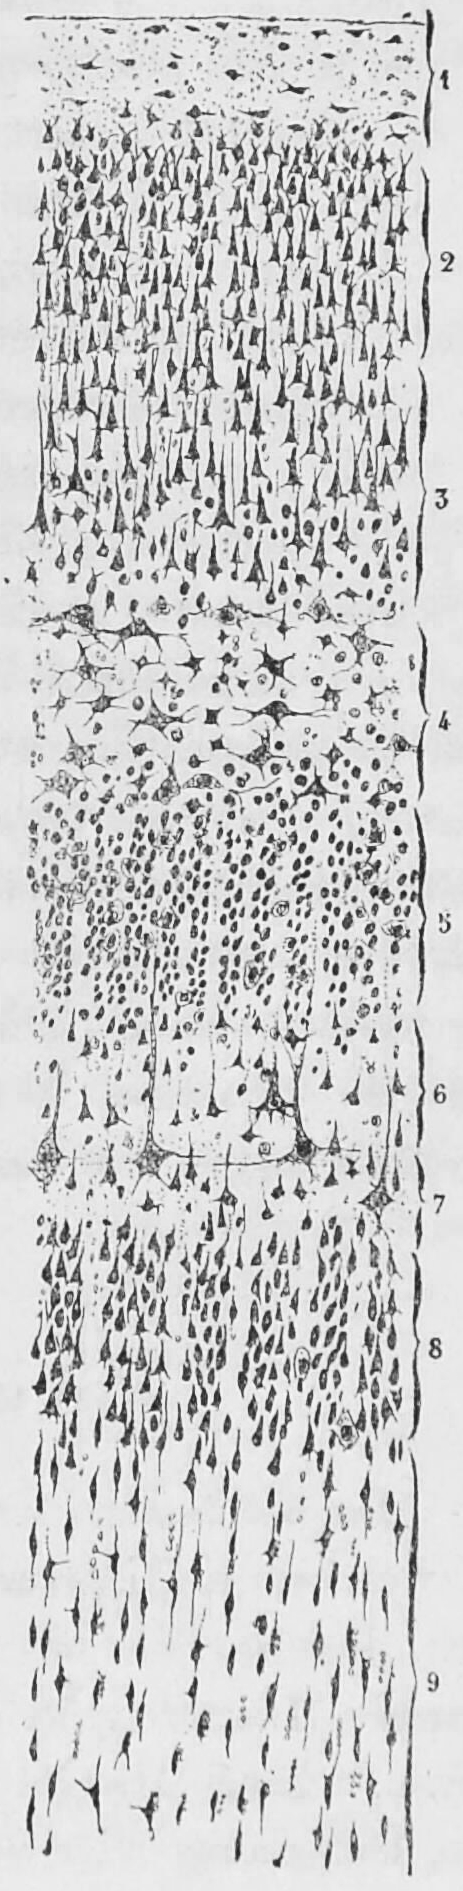
\includegraphics[width=0.7\linewidth]{./figures/cns/cajal_shm_fig1} 

}

\caption{A section of the visual cortex close to the calcarine fissure from the brain of a 29 year old male. Cajal distinguished 9 different layers based on differences of the morpholical features of groups of neurons. \href{https://wellcomelibrary.org/item/b28084585}{Studien über die Hirnrinde des Menschen by S. R. y Cajal}}\label{fig:cajallayers}
\end{figure}

Based on the cytoarchitectural organization of neurons observed using the Nissl method of cell staining, the German anatomist \href{https://en.wikipedia.org/wiki/Korbinian_Brodmann}{Korbinian Brodmann} distinguished in the human cortex 7 major cytoarchitectonic regions (\emph{Hauptregionen} in German; Figure \ref{fig:brodmannregions}) which he subdived into 52 distinct areas (\emph{Felder} in German; Figure \ref{fig:brodmannareas}).



\begin{figure}

{\centering 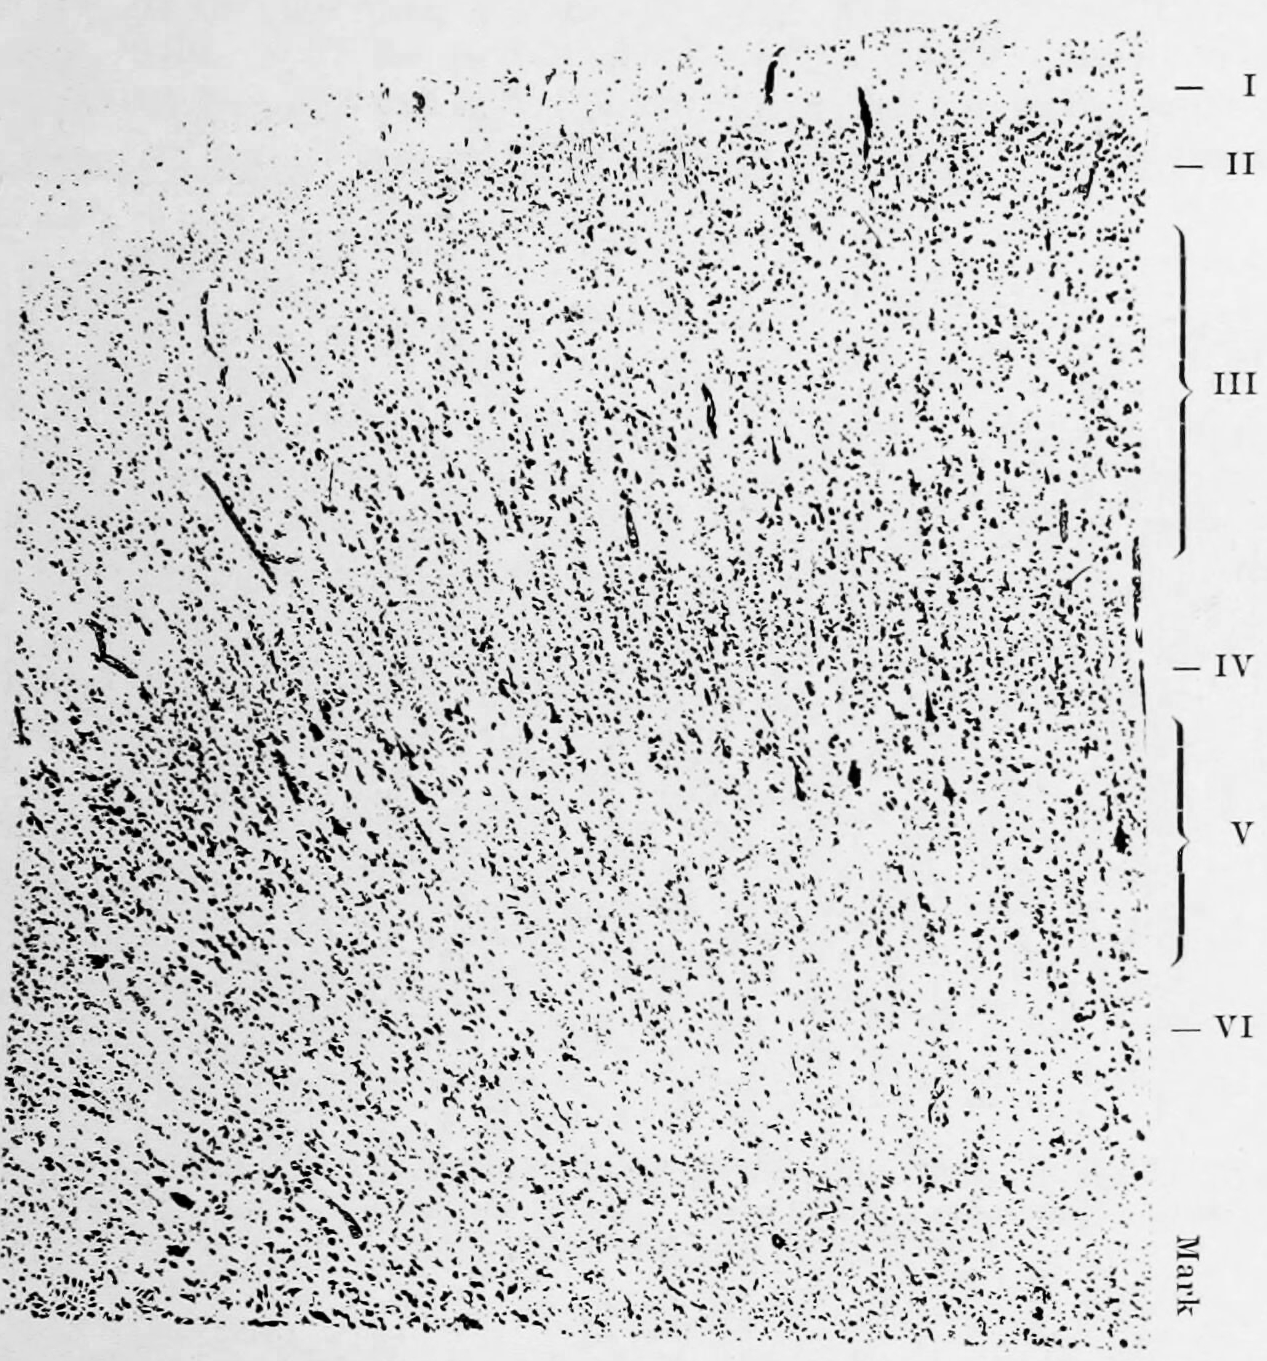
\includegraphics[width=0.7\linewidth]{./figures/cns/cortex_area_5} 

}

\caption{Based on his studies of developing and adult brains of humans and other animals, Korbinian Brodmann proposed that the cerebral cortex consists of six layers. During development and in different brain regions, individual layers can combine or split into sublayers creating location specific cytoarchitectonics. From \href{https://wellcomelibrary.org/item/b28062449}{Broadmann, Korbinian: Vergleichende Lokalisationslehre der Grosshirnrinde in ihren Prinzipien dargestellt auf Grund des Zellenbaues. Verlag von Johann Ambrosius Barth, Leipzig, 1909.}}\label{fig:brodmannlayers}
\end{figure}



\begin{figure}

{\centering 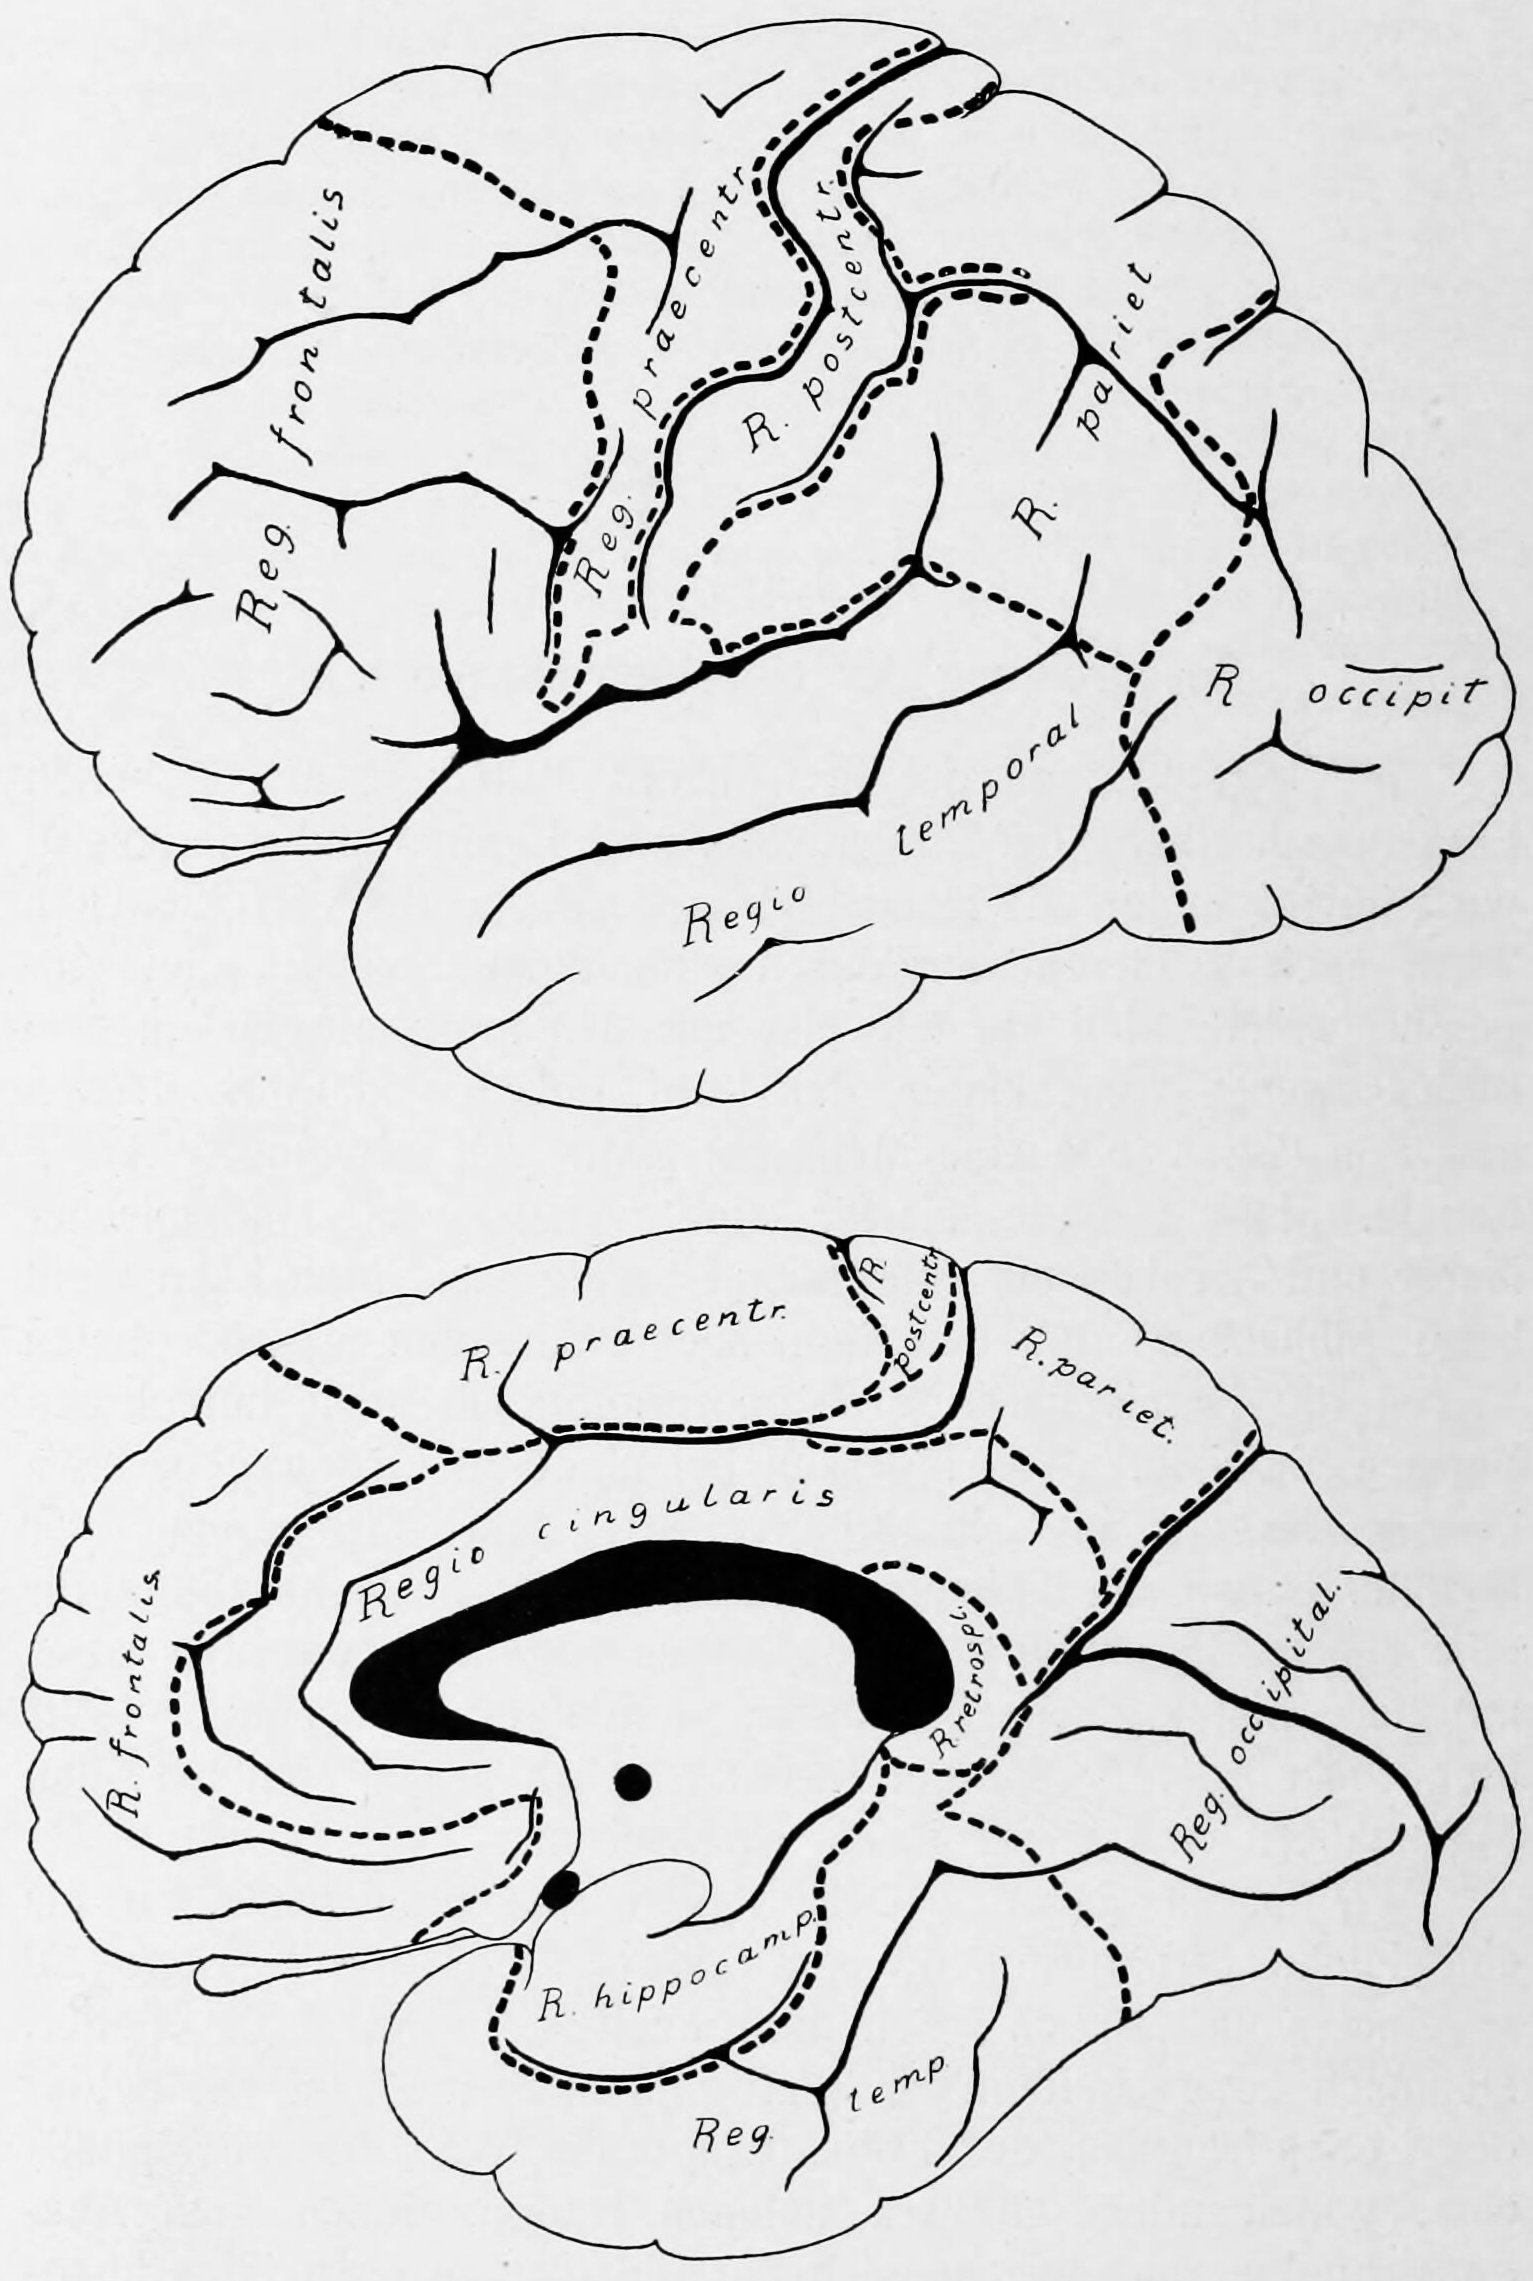
\includegraphics[width=0.7\linewidth]{./figures/cns/Brodmann_hauptregionen} 

}

\caption{\href{https://wellcomelibrary.org/item/b28062449}{Brodmann's diagram of the cerebral cortex showing the 7 major cytoarchitectonic regions that he identified}}\label{fig:brodmannregions}
\end{figure}



\begin{figure}

{\centering 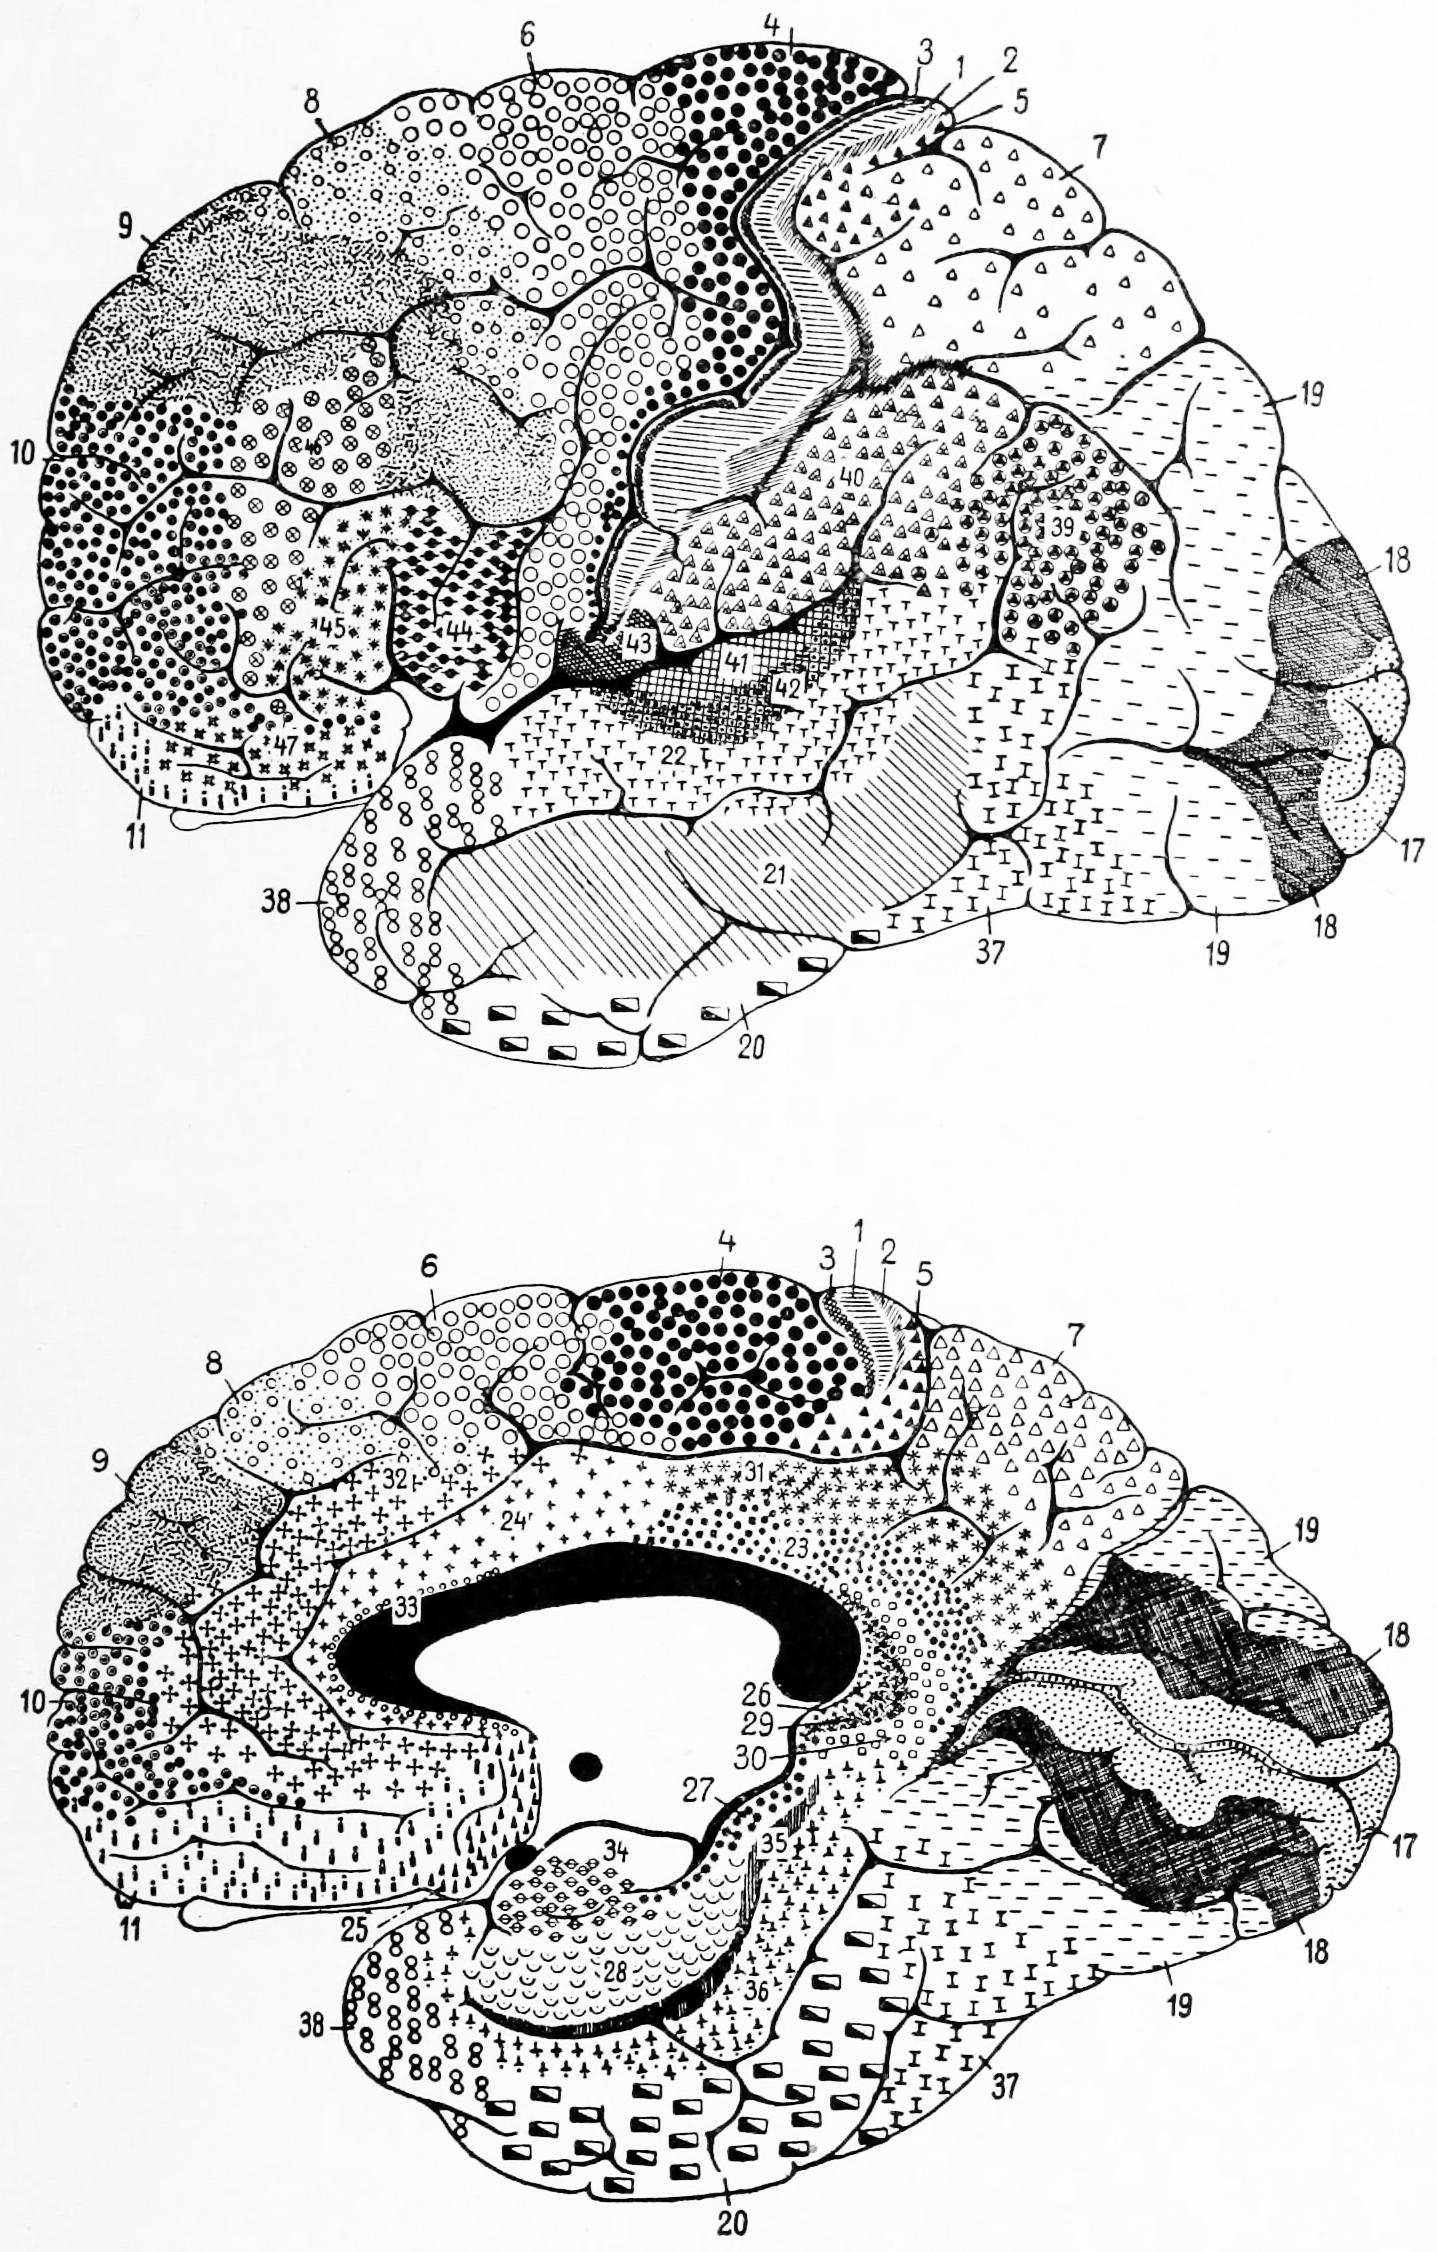
\includegraphics[width=0.7\linewidth]{./figures/cns/Brodmann_original} 

}

\caption{\href{https://wellcomelibrary.org/item/b28062449}{Brodmann's diagram of the cerebral cortex showing the 52 distinct cytoarchitectonic areas he identified}}\label{fig:brodmannareas}
\end{figure}

These areas are distinctly different when seen under a microscope. Brodmann published his maps of cortical areas in humans, monkeys, and other species in 1909, along with many other findings and observations regarding the general cell types and laminar organization of the mammalian cortex. The same Brodmann area number in different species does not necessarily indicate homologous areas. Brodmann postulated that areas with different structures performed different functions. Indeed, some of these areas were later associated to nervous functions, such as the following:

\begin{itemize}
\tightlist
\item
  Brodmann area 41 and 42 in the temporal lobe, related to hearing
\item
  Brodmann area 45 and 44 overlap with the Broca's area for language in humans
\item
  Brodmann area 1, 2, and 3 in the postcentral gyrus of the parietal lobe (the somatosensory region)
\item
  Brodmann area 4 in the precentral gyrus of the frontal lobe (the primary motor area)
\item
  Brodmann area 17 and 18 in the occipital lobe (the primary visual areas).
\end{itemize}

His work to characterize brain cytoarchitecture was strongly influenced by \href{https://en.wikipedia.org/wiki/Oskar_Vogt}{Oskar}, and \href{https://en.wikipedia.org/wiki/Cécile_Vogt-Mugnier}{Cécile} Vogt who postulated over 200 distinct areas in the brain. Another cortical map was published in the two volume work ``Die Cytoarchitektonik der Hirnrinde des erwachsenen Menschen'' (``Cytoarchitectonics of the Adult Human Cerebral Cortex'') by \href{https://en.wikipedia.org/wiki/Constantin_von_Economo}{Constantin von Economo} and \href{https://en.wikipedia.org/wiki/Georg_N._Koskinas}{Georg N. Koskinas} in 1925.



\begin{figure}

{\centering 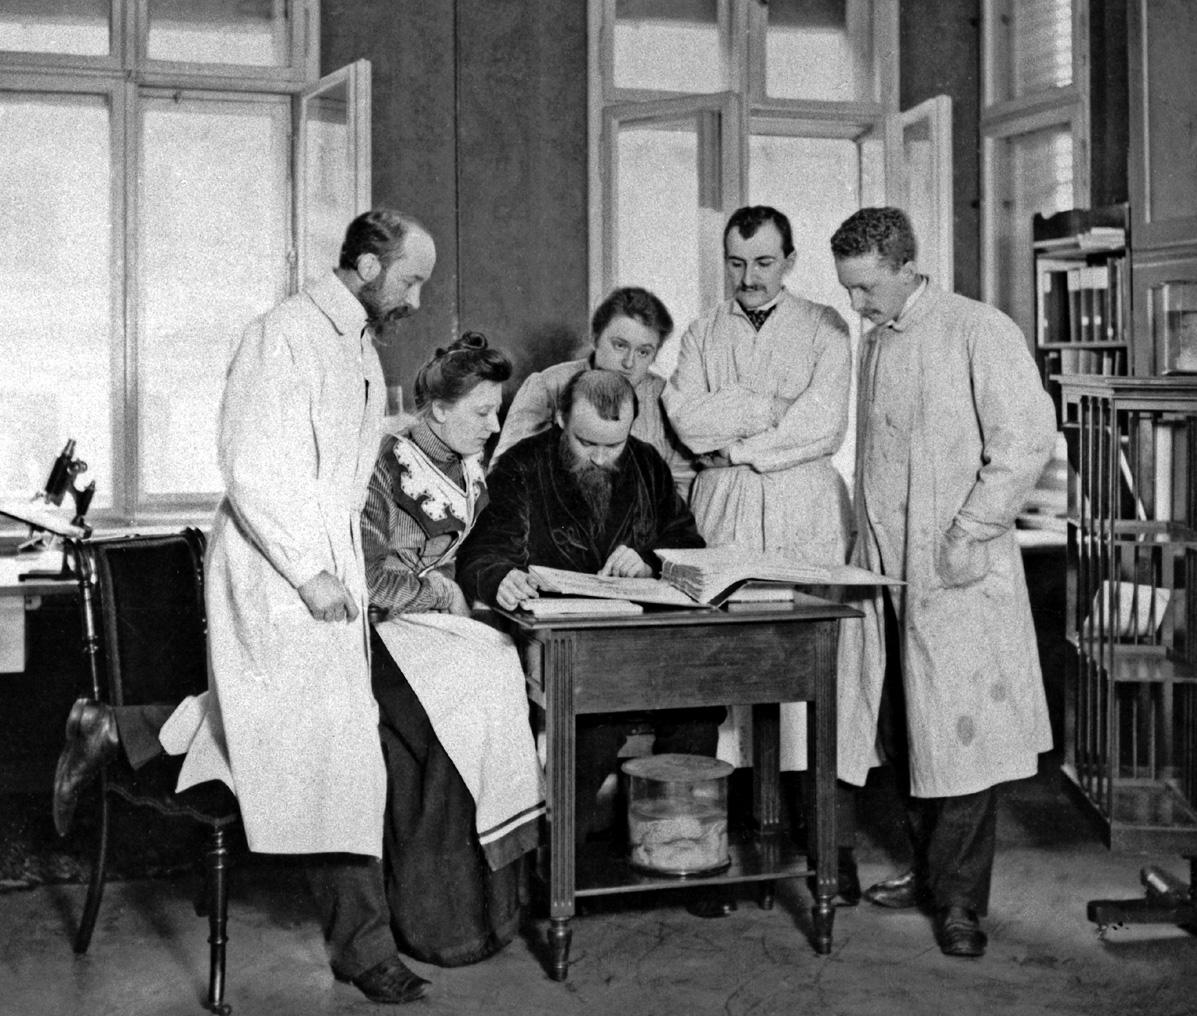
\includegraphics[width=0.7\linewidth]{./figures/cns/Lewandowsky_Vogts_Brodmann} 

}

\caption{\href{https://commons.wikimedia.org/wiki/File:Lewandowsky_Vogts_Brodmann.JPG}{Korbinian Brodmann, Cécile Vogt-Mugnier, Oskar Vogt, Max Borcherdt, and Max Lewandowsky.}}\label{fig:vogtlab}
\end{figure}

Layer I is the molecular layer, and contains few scattered neurons, including GABAergic rosehip neurons. Layer I consists largely of extensions of apical dendritic tufts of pyramidal neurons and horizontally oriented axons, as well as glial cells. During development Cajal-Retzius cells and subpial granular layer cells are present in this layer. Also, some spiny stellate cells can be found here.

Layer II, the external granular layer, contains small pyramidal neurons and numerous stellate neurons.

Layer III, the external pyramidal layer, contains predominantly small and medium-size pyramidal neurons, as well as non-pyramidal neurons with vertically oriented intracortical axons; layers I through III are the main target of interhemispheric corticocortical afferents, and layer III is the principal source of corticocortical efferents.

Layer IV, the internal granular layer, contains different types of stellate and pyramidal cells, and is the main target of thalamocortical afferents from thalamus type C neurons (core-type ) as well as intra-hemispheric corticocortical afferents. The layers above layer IV are also referred to as supragranular layers (layers I-III), whereas the layers below are referred to as infragranular layers (layers V and VI).

Layer V, the internal pyramidal layer, contains large pyramidal neurons. Axons from these leave the cortex and connect with subcortical structures including the basal ganglia. In the primary motor cortex of the frontal lobe, layer V contains giant pyramidal cells called Betz cells, whose axons travel through the internal capsule, the brain stem, and the spinal cord forming the corticospinal tract, which is the main pathway for voluntary motor control.

Layer VI, the polymorphic or multiform layer, contains few large pyramidal neurons and many small spindle-like pyramidal and multiform neurons; layer VI sends efferent fibers to the thalamus, establishing a very precise reciprocal interconnection between the cortex and the thalamus. That is, layer VI neurons from one cortical column connect with thalamus neurons that provide input to the same cortical column. These connections are both excitatory and inhibitory. Neurons send excitatory fibers to neurons in the thalamus and also send collaterals to the thalamic reticular nucleus that inhibit these same thalamus neurons or ones adjacent to them.



\begin{figure}

{\centering 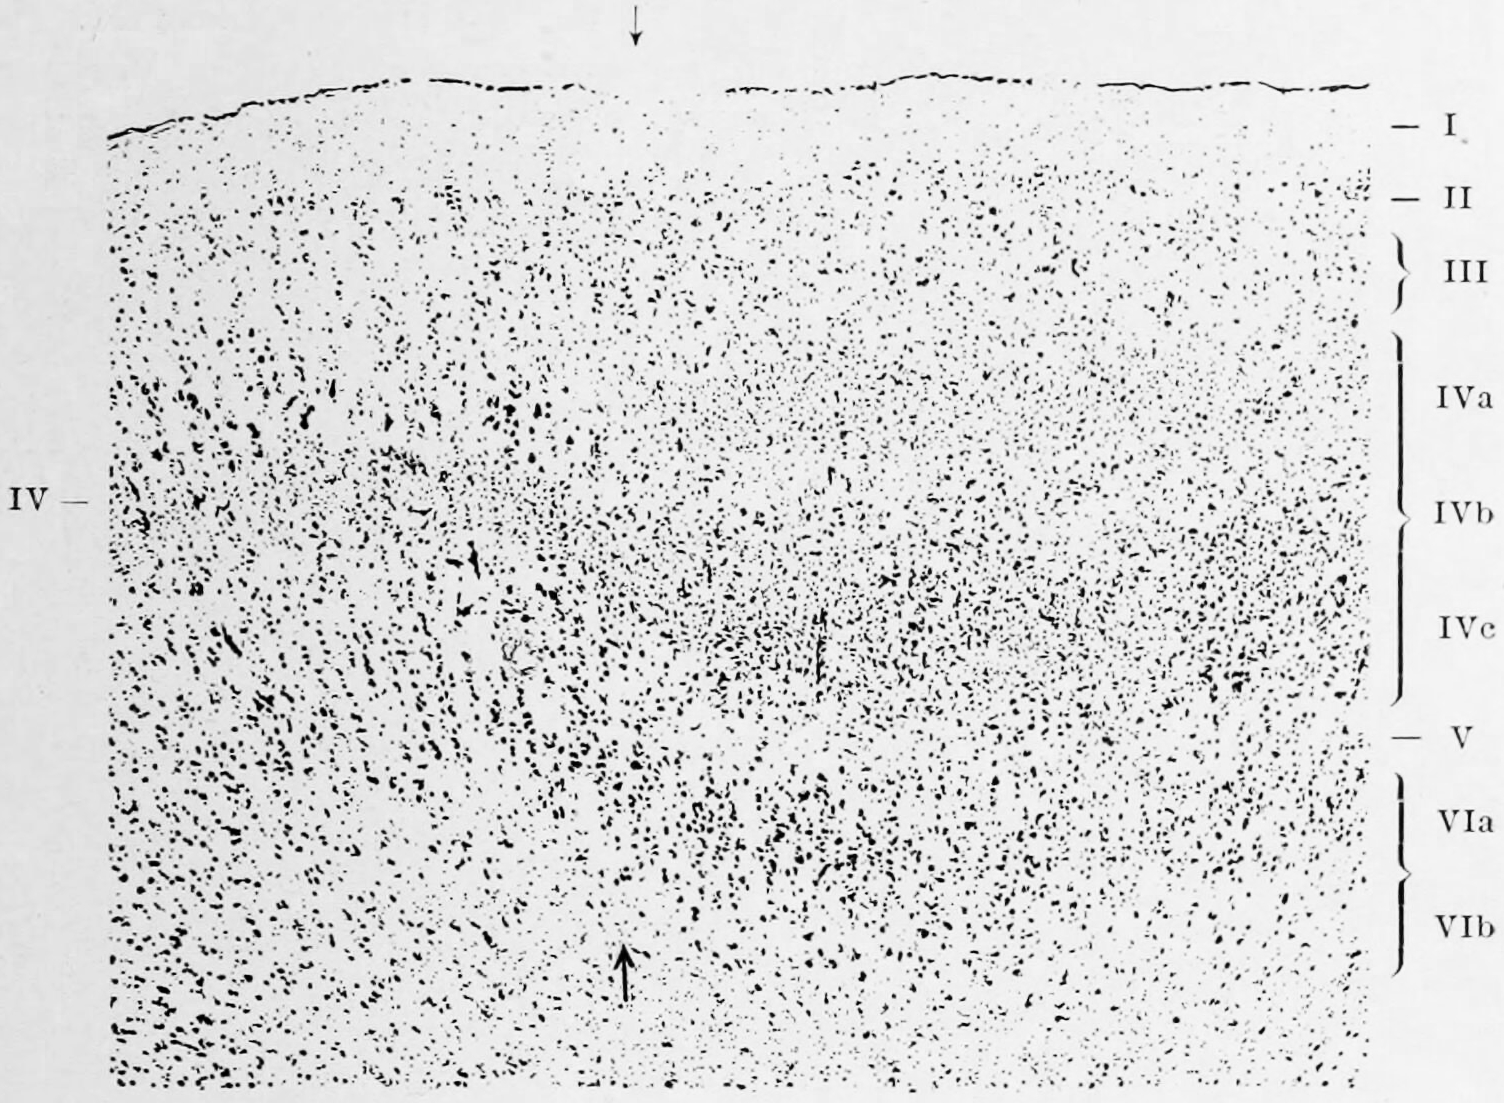
\includegraphics[width=0.7\linewidth]{./figures/cns/cortex_area_17_18} 

}

\caption{The layers in Brodmann areas 17 (towards the right from the arrows) and 18 (towards the left of the arrows) in the human occipital cortex. Like Cajal, Brodmann identified 9 layers (right) in the calcarine area of the visual cortex but in order to fit this observation into this overall scheme of six layers, he chose to subdivide layers 4 and 6. The layers are: I. Lamina zonalis, II. Lamina granularis externa, III Lamina pyramidalis, IV Lamina granularis interna, IVa Sublamina granularis superficialis, IVb Sublamina granularis intermedia, IVc Sublamina granularis interna profunda, V Lamina ganglionaris, VI Lamina multiformis, VIa Sublamina trinagularis, VIb Sublamina fusiformis Sublamina granularis superficialis, IVb Sublamina granularis intermedia, IVc Sublamina granularis interna profunda, V Lamina ganglionaris, VI Lamina multiformis, VIa Sublamina trinagularis, VIb Sublamina fusiformis. \href{https://wellcomelibrary.org/item/b28062449}{Vergleichende Lokalisationslehre der Grosshirnrinde in ihren Prinzipien dargestellt auf Grund des Zellenbaues by K. Brodmann, 1909}}\label{fig:viscortex}
\end{figure}

Many of those brain areas defined by Brodmann have their own complex internal structures. In a number of cases, brain areas are organized into topographic maps, where adjoining bits of the cortex correspond to adjoining parts of the body, or of some more abstract entity. A simple example of this type of correspondence is the primary motor cortex, a strip of tissue running along the anterior edge of the central sulcus. Motor areas innervating each part of the body arise from a distinct zone, with neighboring body parts represented by neighboring zones. Electrical stimulation of the cortex at any point causes a muscle-contraction in the represented body part. This ``somatotopic'' representation is not evenly distributed, however. The head, for example, is represented by a region about three times as large as the zone for the entire back and trunk. The size of any zone correlates to the precision of motor control and sensory discrimination possible. The areas for the lips, fingers, and tongue are particularly large, considering the proportional size of their represented body parts.

In visual areas, the maps are retinotopic; this means they reflect the topography of the retina, the layer of light-activated neurons lining the back of the eye. In this case too, the representation is uneven: the fovea---the area at the center of the visual field---is greatly overrepresented compared to the periphery. The visual circuitry in the human cerebral cortex contains several dozen distinct retinotopic maps, each devoted to analyzing the visual input stream in a particular way. The primary visual cortex (Brodmann area 17), which is the main recipient of direct input from the visual part of the thalamus, contains many neurons that are most easily activated by edges with a particular orientation moving across a particular point in the visual field. Visual areas farther downstream extract features such as color, motion, and shape.

In auditory areas, the primary map is tonotopic. Sounds are parsed according to frequency (i.e., high pitch vs.~low pitch) by subcortical auditory areas, and this parsing is reflected by the primary auditory zone of the cortex. As with the visual system, there are a number of tonotopic cortical maps, each devoted to analyzing sound in a particular way.

Within a topographic map there can sometimes be finer levels of spatial structure. In the primary visual cortex, for example, where the main organization is retinotopic and the main responses are to moving edges, cells that respond to different edge-orientations are spatially segregated from one another.

The cerebral cortex is connected to various subcortical structures such as the thalamus and the basal ganglia, sending information to them along efferent connections and receiving information from them via afferent connections. Most sensory information is routed to the cerebral cortex via the thalamus. Olfactory information, however, passes through the olfactory bulb to the olfactory cortex (piriform cortex).

In more general terms the cortex is typically described as comprising three parts: sensory, motor, and association areas.

The sensory areas are the cortical areas that receive and process information from the senses. Parts of the cortex that receive sensory inputs from the thalamus are called primary sensory areas. The senses of vision, hearing, and touch are served by the primary visual cortex, primary auditory cortex and primary somatosensory cortex respectively. In general, the two hemispheres receive information from the opposite (contralateral) side of the body. For example, the right primary somatosensory cortex receives information from the left limbs, and the right visual cortex receives information from the left visual field. The organization of sensory maps in the cortex reflects that of the corresponding sensing organ, in what is known as a topographic map. Neighboring points in the primary visual cortex, for example, correspond to neighboring points in the retina. This topographic map is called a retinotopic map. In the same way, there exists a tonotopic map in the primary auditory cortex and a somatotopic map in the primary sensory cortex. This last topographic map of the body onto the posterior central gyrus has been illustrated as a deformed human representation, the somatosensory homunculus, where the size of different body parts reflects the relative density of their innervation. Areas with lots of sensory innervation, such as the fingertips and the lips, require more cortical area to process finer sensation.

The motor areas are located in both hemispheres of the cortex. The motor areas are very closely related to the control of voluntary movements, especially fine fragmented movements performed by the hand. The right half of the motor area controls the left side of the body, and vice versa.

Two areas of the cortex are commonly referred to as motor:

\begin{itemize}
\tightlist
\item
  Primary motor cortex, which executes voluntary movements
\item
  Supplementary motor areas and premotor cortex, which select voluntary movements.
\end{itemize}

In addition, motor functions have been described for:

\begin{itemize}
\tightlist
\item
  Posterior parietal cortex, which guides voluntary movements in space
\item
  Dorsolateral prefrontal cortex, which decides which voluntary movements to make according to higher-order instructions, rules, and self-generated thoughts.
\end{itemize}

The association areas are the parts of the cerebral cortex that do not belong to the primary regions. They function to produce a meaningful perceptual experience of the world, enable us to interact effectively, and support abstract thinking and language. The parietal, temporal, and occipital lobes - all located in the posterior part of the cortex - integrate sensory information and information stored in memory. The frontal lobe or prefrontal association complex is involved in planning actions and movement, as well as abstract thought. Globally, the association areas are organized as distributed networks. Each network connects areas distributed across widely spaced regions of the cortex. Distinct networks are positioned adjacent to one another yielding a complex series of interwoven networks. The specific organization of the association networks is debated with evidence for interactions, hierarchical relationships, and competition between networks.

In humans, association networks are particularly important to language function. In the past it was theorized that language abilities are localized in Broca's area in areas of the left inferior frontal gyrus, BA44 and BA45, for language expression and in Wernicke's area BA22, for language reception. However, the processes of language expression and reception have been shown to occur in areas other than just those structures around the lateral sulcus, including the frontal lobe, basal ganglia, cerebellum, and pons.

Below the corpus callosum is the septum pellucidum, a membrane that separates the lateral ventricles. Beneath the lateral ventricles is the thalamus and to the front and below this is the hypothalamus. The hypothalamus leads on to the pituitary gland. At the back of the thalamus is the brainstem.

\hypertarget{the-basal-ganglia}{%
\subsection{The Basal Ganglia}\label{the-basal-ganglia}}

The basal ganglia (or basal nuclei) are a group of subcortical nuclei, of varied origin, in the brains of vertebrates, including humans, which are situated at the base of the forebrain and top of the midbrain, lateral to the thalamus. Basal ganglia are strongly interconnected with the cerebral cortex, thalamus, and brainstem, as well as several other brain areas. The basal ganglia are associated with a variety of functions, including control of voluntary motor movements, procedural learning, habit learning, eye movements, cognition, and emotion.

The main components of the basal ganglia are the caudate nucleus, the putamen, the globus pallidus, the substantia nigra, the nucleus accumbens, and the subthalamic nucleus. The putamen and globus pallidus are also collectively known as the lentiform nucleus, because together they form a lens-shaped body. The putamen and caudate nucleus are also collectively called the corpus striatum after their striped appearance. Part of the dorsal striatum, the putamen, and the globus pallidus, lie separated from the lateral ventricles and thalamus by the internal capsule, whereas the caudate nucleus stretches around and abuts the lateral ventricles on their outer sides. At the deepest part of the lateral sulcus between the insular cortex and the striatum is a thin neuronal sheet called the claustrum.

Below and in front of the striatum are a number of basal forebrain structures. These include the nucleus accumbens, nucleus basalis, diagonal band of Broca, substantia innominata, and the medial septal nucleus.

The main components of the basal ganglia -- as defined functionally -- are the striatum; both dorsal striatum (caudate nucleus and putamen) and ventral striatum (nucleus accumbens and olfactory tubercle), globus pallidus, ventral pallidum, substantia nigra, and subthalamic nucleus. Each of these components has a complex internal anatomical and neurochemical organization. The largest component, the striatum (dorsal and ventral), receives input from many brain areas beyond the basal ganglia, but only sends output to other components of the basal ganglia. The pallidum receives input from the striatum, and sends inhibitory output to a number of motor-related areas. The substantia nigra is the source of the striatal input of the neurotransmitter dopamine, which plays an important role in basal ganglia function. The subthalamic nucleus receives input mainly from the striatum and cerebral cortex, and projects to the globus pallidus.

In more specific terms, the basal ganglia's primary function is likely to control and regulate activities of the motor and premotor cortical areas so that voluntary movements can be performed smoothly. Experimental studies show that the basal ganglia exert an inhibitory influence on a number of motor systems, and that a release of this inhibition permits a motor system to become active. The ``behavior switching'' that takes place within the basal ganglia is influenced by signals from many parts of the brain, including the prefrontal cortex, which plays a key role in executive functions.

The basal ganglia are of major importance for normal brain function and behaviour. Their dysfunction results in a wide range of neurological conditions including disorders of behaviour control and movement. Those of behaviour include Tourette syndrome, obsessive--compulsive disorder, and addiction. Movement disorders include, most notably Parkinson's disease, which involves degeneration of the dopamine-producing cells in the substantia nigra, Huntington's disease, which primarily involves damage to the striatum, dystonia, and more rarely hemiballismus. The basal ganglia have a limbic sector whose components are assigned distinct names: the nucleus accumbens, ventral pallidum, and ventral tegmental area (VTA). There is considerable evidence that this limbic part plays a central role in reward learning as well as cognition and frontal lobe functioning, via the mesolimbic pathway from the VTA to the nucleus accumbens that uses the neurotransmitter dopamine, and the mesocortical pathway. A number of highly addictive drugs, including cocaine, amphetamine, specific medications that are prescribed by a doctor, and nicotine, are thought to work by increasing the efficacy of this dopamine signal. There is also evidence implicating overactivity of the VTA dopaminergic projection in schizophrenia.

\hypertarget{the-limbic-lobe}{%
\subsection{The Limbic Lobe}\label{the-limbic-lobe}}

The limbic lobe is an arc-shaped region of cortex on the medial surface of each cerebral hemisphere of the mammalian brain, consisting of parts of the frontal, parietal and temporal lobes. The term limbic comes from the Latin limbus, for ``border'' or ``edge'', or, particularly in medical terminology, a border of an anatomical component.

\href{https://en.wikipedia.org/wiki/Paul_Broca}{Pierre Paul Broca} first called this part of the brain le grand lobe limbique in 1878. He examined the differentiation between deeply recessed cortical tissue and underlying, subcortical nuclei.

Broca identified the limbic lobe with the cingulate and parahippocampal gyri, and associated it with the sense of smell.

The limbic system is a term that was introduced in 1949 by the American physician and neuroscientist, Paul D. MacLean. The In 1937, \href{https://en.wikipedia.org/wiki/James_Papez}{James Papez} proposed that the circuit connecting the hypothalamus to the limbic lobe was the basis for emotional experiences. Papez had been studying cases of rabies which is a disease that causes high levels of aggression. He noticed that this heightened aggression correlated with damage to the hippocampus. Theoretically, this made sense to Papez who asserted that the hippocampus is responsible for the expression of emotion because of its connection to the autonomic nervous system. He also noticed that in other cases, certain stimuli (taste, smell, pain, etc.) would cause strong emotional responses. These stimuli activated not only the hippocampus but also other brain structures. He theorized that these brain structures worked together as the emotional control center in the brain. These interconnected structures were subsequently referred to as the the Papez circuit. Because of these studies, Papez strongly believed that the circuit was the cortical control of emotion. Further evidence that the limbic system was responsible for the cortical representation of emotions was discovered in 1939, by Heinrich Kluver and Paul Bucy. Kluver and Bucy, after much research, demonstrated that the bilateral removal of the temporal lobes in monkeys created an extreme behavioral syndrome. After performing a temporal lobectomy, the monkeys showed a decrease in aggression. The animals revealed a reduced threshold to visual stimuli, and were thus unable to recognize objects that were once familiar.



\begin{figure}

{\centering \includegraphics[width=0.7\linewidth]{./figures/cns/papez_circuit} 

}

\caption{Schematic briefly summarizing neural systems proposed to process emotion, highlighting structures that are visible on the medial surface of the brain. Papez's (1937) original circuit (A) was expanded upon in the concept of the limbic system (B) to include a variety of subcortical and cortical territories (MacLean, 1952; Heimer and Van Hoesen, 2006). (Structures like the anterior insula and nucleus basalis of Meynert, which are not visible on the medial surface of the brain, are not represented here). Images modified from Papez's original drawing. From Barger N, Hanson KL, Teffer K, Schenker-Ahmed NM and Semendeferi K (2014) Evidence for evolutionary specialization in human limbic structures. \href{http://journal.frontiersin.org/article/10.3389/fnhum.2014.00277/full}{Front. Hum. Neurosci. 8:277. doi: 10.3389/fnhum.2014.00277}}\label{fig:papezcircuit}
\end{figure}

Around the same time, \href{https://en.wikipedia.org/wiki/Paul_D._MacLean}{Paul D. MacLean} was also interested in the Papez circuit. He had read through Paul Broca's research which indicated that the limbic lobe that surrounds the brainstem is a structure present in all mammals. Papez's paper on the emotional circuit which involved the connection between the hypothalamus and the limbic lobe set MacLean on a journey to learn more. He visited Papez at Cornell University after which he proposed a modified version of the Papez circuit in 1952, emphasizing not only the hippocampus, but also the amygdala and septum.

The hippocampus, amygdala, and septum make up the rhinencephalon (frontotemporal portion of the brain) or, as the Bavarian neuropathologist Christfried Jakob had termed it in 1907/1908, the visceral brain. Together, the limbic lobe and the visceral brain make up the limbic system. MacLean believed that including the visceral brain in the limbic system accounted for the external sensory information associated with subjective emotional experiences. MacLean coined the term limbic system.

There is controversy over the use of the term limbic system, with some scientists arguing that the term be considered obsolete and abandoned. Originally, the limbic system was believed to be the emotional center of the brain, with cognition being the business of the neocortex. However, cognition depends on acquisition and retention of memories, in which the hippocampus, a primary limbic interacting structure, is involved: hippocampus damage causes severe cognitive (memory) deficits. More important, the ``boundaries'' of the limbic system have been repeatedly redefined because of advances in neuroscience. Therefore, while it is true that limbic interacting structures are more closely related to emotion, the limbic system itself is best thought of as a component of a larger emotional processing plant, that is essentially responsible for sifting through, organizing, lower order processing, and relaying sensory information to other brain areas for higher order emotional processing.

\hypertarget{the-hippocampus}{%
\subsection{The Hippocampus}\label{the-hippocampus}}

The hippocampus is located under the cerebral cortex in the allocortex, and in primates it is in the medial temporal lobe. It contains two main interlocking parts: the hippocampus proper (also called Ammon's horn) and the dentate gyrus. It is involved with various processes relating to cognition and is one of the most well understood and heavily involved limbic interacting structure.

The earliest description of the ridge running along the floor of the temporal horn of the lateral ventricle comes from the Venetian anatomist Julius Caesar Aranzi (1587), who likened it first to a silkworm and then to a seahorse (Latin hippocampus, from Greek ἱππόκαμπος, from Greek ἵππος, ``horse'' + κάμπος, ``sea-monster''). The German anatomist Duvernoy (1729), the first to illustrate the structure, also wavered between ``seahorse'' and ``silkworm''. ``Ram's horn'' was proposed by the Danish anatomist Jacob Winsløw in 1732; and a decade later his fellow Parisian, the surgeon de Garengeot, used ``cornu Ammonis'' -- horn of (the ancient Egyptian god) Amun, who was often represented as having a ram's head. This has survived in abbreviated form as CA in naming the subfields of the hippocampus.



\begin{figure}

{\centering \includegraphics[width=0.7\linewidth]{./figures/cns/Hippocampus_and_seahorse} 

}

\caption{\href{https://commons.wikimedia.org/wiki/File:Hippocampus_and_seahorse.JPG}{A human hippocampus alongside a sea horse.}}\label{fig:seahorse}
\end{figure}

Another reference appeared with the term pes hippocampi, which may date back to Diemerbroeck in 1672, introducing a comparison with the shape of the folded back forelimbs and webbed feet of the mythological hippocampus, a sea-monster with a horse's forequarters and a fish's tail. The hippocampus was then described as pes hippocampi major, with an adjacent bulge in the occipital horn, described as the pes hippocampi minor and later renamed as the calcar avis. The renaming of the hippocampus as hippocampus major, and the calcar avis as hippocampus minor, has been attributed to Félix Vicq-d'Azyr systematising nomenclature of parts of the brain in 1786. Mayer mistakenly used the term hippopotamus in 1779, and was followed by some other authors until Karl Friedrich Burdach resolved this error in 1829. In 1861 the hippocampus minor became the centre of a dispute over human evolution between Thomas Henry Huxley and Richard Owen, satirised as the Great Hippocampus Question. The term hippocampus minor fell from use in anatomy textbooks, and was officially removed in the Nomina Anatomica of 1895. Today, the structure is just called the hippocampus, with the term Cornu Ammonis surviving in the names of the hippocampal subfields CA1-CA4.

Since different neuronal cell types are neatly organized into layers in the hippocampus, it has frequently been used as a model system for studying neurophysiology. The form of neural plasticity known as long-term potentiation (LTP) was initially discovered to occur in the hippocampus and has often been studied in this structure. LTP is widely believed to be one of the main neural mechanisms by which memories are stored in the brain.



\begin{figure}

{\centering \includegraphics[width=0.7\linewidth]{./figures/cns/Sobo_1909_646} 

}

\caption{Coronal section of the brain of a macaque monkey, showing the hippocampus. From \href{https://commons.wikimedia.org/wiki/File:Sobo_1909_634.png}{Sobotta's Textbook and Atlas of Human Anatomy 1909}}\label{fig:hippocross}
\end{figure}

In rodents as model organisms, the hippocampus has been studied extensively as part of a brain system responsible for spatial memory and navigation. Many neurons in the rat and mouse hippocampus respond as place cells: that is, they fire bursts of action potentials when the animal passes through a specific part of its environment. Hippocampal place cells interact extensively with head direction cells, whose activity acts as an inertial compass, and conjecturally with grid cells in the neighboring entorhinal cortex.

Spatial memory was found to have many sub-regions in the hippocampus, such as the dentate gyrus (DG) in the dorsal hippocampus, the left hippocampus, and the parahippocampal region. The dorsal hippocampus was found to be an important component for the generation of new neurons, called adult-born granules (GC), in adolescence and adulthood. These new neurons contribute to pattern separation in spatial memory, increasing the firing in cell networks, and overall causing stronger memory formations. This is thought to integrate spatial and episodic memories with the limbic system via a feedback loop that provides emotional context of a particular sensory input.



\begin{figure}

{\centering \includegraphics[width=0.7\linewidth]{./figures/cns/CajalHippocampus} 

}

\caption{Diagram of the structure and connections of the hippocampus. A, Molecular layer of the subiculum. B, Pyramidal cell layer of the Subiculum. C, Hippocampus. D, Fascia dentata. E, Fimbria. F, Cingulum. G, H, Corpus callosum. a, axons entering the cingulum. From \href{https://wellcomelibrary.org/item/b2129592x\#?c=0\&m=0\&s=0\&cv=14\&z=0\%2C-3.48\%2C1\%2C8.6591}{Histologie du système nerveux de l'homme \& des vertébrés, Tome Premier} (1909) by Santiago Ramón y Cajal translated from Spanish by Dr.~L. Azoulay.}\label{fig:hippocircuit}
\end{figure}

Damage related to the hippocampal region of the brain has reported vast effects on overall cognitive functioning, particularly memory such as spatial memory. As previously mentioned, spatial memory is a cognitive function greatly intertwined with the hippocampus. While damage to the hippocampus may be a result of a brain injury or other injuries of that sort, researchers particularly investigated the effects that high emotional arousal and certain types of drugs had on the recall ability in this specific memory type. In particular, in a study performed by Parkard, rats were given the task of correctly making their way through a maze. In the first condition, rats were stressed by shock or restraint which caused a high emotional arousal. When completing the maze task, these rats had an impaired effect on their hippocampal-dependent memory when compared to the control group. Then, in a second condition, a group of rats were injected with anxiogenic drugs. Like the former these results reported similar outcomes, in that hippocampal-memory was also impaired. Studies such as these reinforce the impact that the hippocampus has on memory processing, in particular the recall function of spatial memory. Furthermore, impairment to the hippocampus can occur from prolonged exposure to stress hormones such as glucocorticoids (GCs), which target the hippocampus and cause disruption in explicit memory.

In an attempt to curtail life-threatening epileptic seizures, 27-year-old Henry Gustav Molaison underwent bilateral removal of almost all of his hippocampus in 1953. Over the course of fifty years he participated in thousands of tests and research projects that provided specific information on exactly what he had lost. Semantic and episodic events faded within minutes, having never reached his long term memory, yet emotions, unconnected from the details of causation, were often retained. Dr.~Suzanne Corkin, who worked with him for 46 years until his death, described the contribution of this tragic ``experiment'' in her 2013 book.

\hypertarget{the-amygdala}{%
\subsection{The Amygdala}\label{the-amygdala}}

Another integrative part of the limbic system, the amygdala, which is deepest part of the limbic system, is involved in many cognitive processes and is largely considered the most primordial and vital part of the limbic system. Like the hippocampus, processes in the amygdala seem to impact memory; however, it is not spatial memory as in the hippocampus but the semantic division of episodic-autobiographical memory (EAM) networks. Markowitsch's amygdala research shows it encodes, stores, and retrieves EAM memories. To delve deeper into these types of processes by the amygdala, Markowitsch and his team provided extensive evidence through investigations that the ``amygdala's main function is to charge cues so that mnemonic events of a specific emotional significance can be successfully searched within the appropriate neural nets and re-activated.'' These cues for emotional events created by the amygdala encompass the EAM networks previously mentioned.

Besides memory, the amygdala also seems to be an important brain region involved in attentional and emotional processes. First, to define attention in cognitive terms, attention is the ability to focus on some stimuli while ignoring others. Thus, the amygdala seems to be an important structure in this ability. Foremost, however, this structure was historically thought to be linked to fear, allowing the individual to take action in response to that fear. However, as time has gone by, researchers such as Pessoa, generalized this concept with help from evidence of EEG recordings, and concluded that the amygdala helps an organism to define a stimulus and therefore respond accordingly. However, when the amygdala was initially thought to be linked to fear, this gave way for research in the amygdala for emotional processes. Kheirbek demonstrated research that the amygdala is involved in emotional processes, in particular the ventral hippocampus. He described the ventral hippocampus as having a role in neurogenesis and the creation of adult-born granule cells (GC). These cells not only were a crucial part of neurogenesis and the strengthening of spatial memory and learning in the hippocampus but also appear to be an essential component to the function of the amygdala. A deficit of these cells, as Pessoa (2009) predicted in his studies, would result in low emotional functioning, leading to high retention rate of mental diseases, such as anxiety disorders.

Social processing, specifically the evaluation of faces in social processing, is an area of cognition specific to the amygdala. In a study done by Todorov, fMRI tasks were performed with participants to evaluate whether the amygdala was involved in the general evaluation of faces. After the study, Todorov concluded from his fMRI results that the amygdala did indeed play a key role in the general evaluation of faces. However, in a study performed by researchers Koscik and his team, the trait of trustworthiness was particularly examined in the evaluation of faces. Koscik and his team demonstrated that the amygdala was involved in evaluating the trustworthiness of an individual. They investigated how brain damage to the amygdala played a role in trustworthiness, and found that individuals that suffered damage tended to confuse trust and betrayal, and thus placed trust in those having done them wrong. Furthermore, Rule, along with his colleagues, expanded on the idea of the amygdala in its critique of trustworthiness in others by performing a study in 2009 in which he examined the amygdala's role in evaluating general first impressions and relating them to real-world outcomes. Their study involved first impressions of CEOs. Rule demonstrated that while the amygdala did play a role in the evaluation of trustworthiness, as observed by Koscik in his own research two years later in 2011, the amygdala also played a generalized role in the overall evaluation of first impression of faces. This latter conclusion, along with Todorov's study on the amygdala's role in general evaluations of faces and Koscik's research on trustworthiness and the amygdala, further solidified evidence that the amygdala plays a role in overall social processing.

\hypertarget{the-thalamus}{%
\subsection{The Thalamus}\label{the-thalamus}}

The thalamus (from Greek θάλαμος, ``chamber'') is a large mass of gray matter located in the dorsal part of the diencephalon. Nerve fibers project out of the thalamus to the cerebral cortex in all directions, allowing hub-like exchanges of information.

Anatomically, it is a midline symmetrical structure of two halves (left and right), within the vertebrate brain, situated between the cerebral cortex and the midbrain. It forms during embryonic development as the main product of the diencephalon, as first recognized by the Swiss embryologist and anatomist \href{https://en.wikipedia.org/wiki/Wilhelm_His_Sr.}{Wilhelm His Sr.} in 1893.

The thalamus has many connections to the hippocampus via the mammillothalamic tract, this tract comprises the mammillary bodies and fornix.



\begin{figure}

{\centering \includegraphics[width=0.7\linewidth]{./figures/cns/Sobo_1909_634} 

}

\caption{View of the left hemisphere from medial and below with the brainstem and cerebellum removed by an oblique section through the thalamus. The entire fornix is visible as are the mammilary body. \href{https://commons.wikimedia.org/wiki/File:Sobo_1909_634.png}{Sobotta's Textbook and Atlas of Human Anatomy 1909}}\label{fig:thalamusview}
\end{figure}

The thalamus is connected to the cerebral cortex via the thalamocortical radiations.

The spinothalamic tract is a sensory pathway originating in the spinal cord. It transmits information to the thalamus about pain, temperature, itch and crude touch. There are two main parts: the lateral spinothalamic tract, which transmits pain and temperature, and the anterior (or ventral) spinothalamic tract, which transmits crude touch and pressure.

The thalamus has multiple functions, generally believed to act as a relay station, or hub, relaying information between different subcortical areas and the cerebral cortex. In particular, every sensory system (with the exception of the olfactory system) includes a thalamic nucleus that receives sensory signals and sends them to the associated primary cortical area. For the visual system, for example, inputs from the retina are sent to the lateral geniculate nucleus of the thalamus, which in turn projects to the visual cortex in the occipital lobe. The thalamus is believed to both process sensory information as well as relay it---each of the primary sensory relay areas receives strong feedback connections from the cerebral cortex. Similarly the medial geniculate nucleus acts as a key auditory relay between the inferior colliculus of the midbrain and the primary auditory cortex. The ventral posterior nucleus is a key somatosensory relay, which sends touch and proprioceptive information to the primary somatosensory cortex.

\hypertarget{the-hypothalamus}{%
\subsection{The Hypothalamus}\label{the-hypothalamus}}

The hypothalamus is a portion of the brain that contains a number of small nuclei with a variety of functions. One of the most important functions of the hypothalamus is to link the nervous system to the endocrine system via the pituitary gland. The hypothalamus is located below the thalamu. It forms the ventral part of the diencephalon. All vertebrate brains contain a hypothalamus. In humans, it is the size of an almond. The hypothalamus is responsible for the regulation of certain metabolic processes and other activities of the autonomic nervous system. It synthesizes and secretes certain neurohormones, called releasing hormones or hypothalamic hormones, and these in turn stimulate or inhibit the secretion of hormones from the pituitary gland. The hypothalamus controls body temperature, hunger, important aspects of parenting and attachment behaviours, thirst, fatigue, sleep, and circadian rhythms. The hypothalamus derives its name from Greek ὑπό, under and θάλαμος, chamber.

The hypothalamus is a divided into 3 regions (supraoptic, tuberal, mammillary) in a parasagittal plane, indicating location anterior-posterior; and 3 areas (periventricular, medial, lateral) in the coronal plane, indicating location medial-lateral. Hypothalamic nuclei are located within these specific regions and areas. It is found in all vertebrate nervous systems. In mammals, magnocellular neurosecretory cells in the paraventricular nucleus and the supraoptic nucleus of the hypothalamus produce neurohypophysial hormones, oxytocin and vasopressin. These hormones are released into the blood in the posterior pituitary. Much smaller parvocellular neurosecretory cells, neurons of the paraventricular nucleus, release corticotropin-releasing hormone and other hormones into the hypophyseal portal system, where these hormones diffuse to the anterior pituitary.

The hypothalamus is highly interconnected with other parts of the central nervous system, in particular the brainstem and its reticular formation. As part of the limbic system, it has connections to other limbic structures including the amygdala and septum, and is also connected with areas of the autonomous nervous system.

The hypothalamus has a central neuroendocrine function, most notably by its control of the anterior pituitary, which in turn regulates various endocrine glands and organs. Releasing hormones (also called releasing factors) are produced in hypothalamic nuclei then transported along axons to either the median eminence or the posterior pituitary, where they are stored and released as needed.

The hypothalamus has a central neuroendocrine function, most notably by its control of the anterior pituitary, which in turn regulates various endocrine glands and organs. Releasing hormones (also called releasing factors) are produced in hypothalamic nuclei then transported along axons to either the median eminence or the posterior pituitary, where they are stored and released as needed.

In the hypothalamic--adenohypophyseal axis, releasing hormones, also known as hypophysiotropic or hypothalamic hormones, are released from the median eminence, a prolongation of the hypothalamus, into the hypophyseal portal system, which carries them to the anterior pituitary where they exert their regulatory functions on the secretion of adenohypophyseal hormones. These hypophysiotropic hormones are stimulated by parvocellular neurosecretory cells located in the periventricular area of the hypothalamus. After their release into the capillaries of the third ventricle, the hypophysiotropic hormones travel through what is known as the hypothalamo-pituitary portal circulation. Once they reach their destination in the anterior pituitary, these hormones bind to specific receptors located on the surface of pituitary cells. Depending on which cells are activated through this binding, the pituitary will either begin secreting or stop secreting hormones into the rest of the bloodstream.

Other hormones secreted from the median eminence include vasopressin, oxytocin, and neurotensin.

In the hypothalamic-neurohypophyseal axis, neurohypophysial hormones are released from the posterior pituitary, which is actually a prolongation of the hypothalamus, into the circulation. It is also known that hypothalamic-pituitary-adrenal axis (HPA) hormones are related to certain skin diseases and skin homeostasis. There is evidence linking hyperactivity of HPA hormones to stress-related skin diseases and skin tumors.

The extreme lateral part of the ventromedial nucleus of the hypothalamus is responsible for the control of food intake. Stimulation of this area causes increased food intake. Bilateral lesion of this area causes complete cessation of food intake. Medial parts of the nucleus have a controlling effect on the lateral part. Bilateral lesion of the medial part of the ventromedial nucleus causes hyperphagia and obesity of the animal. Further lesion of the lateral part of the ventromedial nucleus in the same animal produces complete cessation of food intake.

There are different hypotheses related to this regulation:

\begin{itemize}
\tightlist
\item
  Lipostatic hypothesis: This hypothesis holds that adipose tissue produces a humoral signal that is proportionate to the amount of fat and acts on the hypothalamus to decrease food intake and increase energy output. It has been evident that a hormone leptin acts on the hypothalamus to decrease food intake and increase energy output.
\item
  Gutpeptide hypothesis: gastrointestinal hormones like Grp, glucagons, CCK and others claimed to inhibit food intake. The food entering the gastrointestinal tract triggers the release of these hormones, which act on the brain to produce satiety. The brain contains both CCK-A and CCK-B receptors.
\item
  Glucostatic hypothesis: The activity of the satiety center in the ventromedial nuclei is probably governed by the glucose utilization in the neurons. It has been postulated that when their glucose utilization is low and consequently when the arteriovenous blood glucose difference across them is low, the activity across the neurons decrease. Under these conditions, the activity of the feeding center is unchecked and the individual feels hungry. Food intake is rapidly increased by intraventricular administration of 2-deoxyglucose therefore decreasing glucose utilization in cells.
\item
  Thermostatic hypothesis: According to this hypothesis, a decrease in body temperature below a given set-point stimulates appetite, whereas an increase above the set-point inhibits appetite.
\end{itemize}

\hypertarget{the-brainstem}{%
\subsection{The Brainstem}\label{the-brainstem}}

The brainstem lies beneath the cerebrum and consists of the midbrain, pons and medulla. It lies in the back part of the skull, resting on the part of the base known as the clivus, and ends at the foramen magnum, a large opening in the occipital bone. The brainstem continues below this as the spinal cord, protected by the vertebral column.



\begin{figure}

{\centering \includegraphics[width=0.7\linewidth]{./figures/cns/Sobotta_1909_660} 

}

\caption{View of the brainstem from behind (left) and from the left (right). \href{https://commons.wikimedia.org/wiki/File:Sobo_1909_660.png}{Sobotta's Textbook and Atlas of Human Anatomy 1909}}\label{fig:quadrigemina}
\end{figure}

Ten of the twelve pairs of cranial nerves emerge directly from the brainstem. The brainstem also contains many cranial nerve nuclei and nuclei of peripheral nerves, as well as nuclei involved in the regulation of many essential processes including breathing, control of eye movements and balance. The reticular formation, a network of nuclei of ill-defined formation, is present within and along the length of the brainstem. Many nerve tracts, which transmit information to and from the cerebral cortex to the rest of the body, pass through the brainstem.

The internal carotid arteries supply oxygenated blood to the front of the brain and the vertebral arteries supply blood to the back of the brain. These two circulations join together in the circle of Willis, a ring of connected arteries that lies in the interpeduncular cistern between the midbrain and pons.



\begin{figure}

{\centering \includegraphics[width=0.7\linewidth]{./figures/cns/GrayAnat1918p572} 

}

\caption{The arteries of the base of the brain. The tempora pole of the cerebrum and a portion of the cerebellar hemisphere have been removed on the right side. From \href{https://archive.org/details/anatomyofhumanbo1918gray/page/n6/mode/2up}{Gray Henry, Anatomy of the Human Body. 20\textsuperscript{th} Edition, Lea \& Febiger, Philadelphia \& New York, 1918}}\label{fig:bloodsupply}
\end{figure}

The internal carotid arteries are branches of the common carotid arteries. They enter the cranium through the carotid canal, travel through the cavernous sinus and enter the subarachnoid space. They then enter the circle of Willis, with two branches, the anterior cerebral arteries emerging. These branches travel forward and then upward along the longitudinal fissure, and supply the front and midline parts of the brain. One or more small anterior communicating arteries join the two anterior cerebral arteries shortly after they emerge as branches. The internal carotid arteries continue forward as the middle cerebral arteries. They travel sideways along the sphenoid bone of the eye socket, then upwards through the insula cortex, where final branches arise. The middle cerebral arteries send branches along their length.



\begin{figure}

{\centering \includegraphics[width=0.7\linewidth]{./figures/cns/GrayAnat1918p574} 

}

\caption{Diagram of the arterial circulation at the base of the brain. A.L. Antero-lateral. A.M. Antero-medial.P.L. Postero-lateral. P.M. Postero-medial ganglionic branches. From \href{https://archive.org/details/anatomyofhumanbo1918gray/page/n6/mode/2up}{Gray Henry, Anatomy of the Human Body. 20\textsuperscript{th} Edition, Lea \& Febiger, Philadelphia \& New York, 1918}}\label{fig:bloodsupplydiagram}
\end{figure}

The vertebral arteries emerge as branches of the left and right subclavian arteries. They travel upward through transverse foramina which are spaces in the cervical vertebrae. Each side enters the cranial cavity through the foramen magnum along the corresponding side of the medulla. They give off one of the three cerebellar branches. The vertebral arteries join in front of the middle part of the medulla to form the larger basilar artery, which sends multiple branches to supply the medulla and pons, and the two other anterior and superior cerebellar branches. Finally, the basilar artery divides into two posterior cerebral arteries. These travel outwards, around the superior cerebellar peduncles, and along the top of the cerebellar tentorium, where it sends branches to supply the temporal and occipital lobes. Each posterior cerebral artery sends a small posterior communicating artery to join with the internal carotid arteries.

\hypertarget{the-midbrain}{%
\subsection{The Midbrain}\label{the-midbrain}}

The midbrain or mesencephalon is the rostral-most portion of the brainstem and is associated with vision, hearing, motor control, sleep and wakefulness, arousal (alertness), and temperature regulation.

The principal regions of the midbrain are the tectum, the cerebral aqueduct, tegmentum, and the cerebral peduncles. Rostrally the midbrain adjoins the diencephalon (thalamus, hypothalamus, etc.), while caudally it adjoins the hindbrain (pons, medulla and cerebellum). In the rostral direction, the midbrain noticeably splays laterally.

\hypertarget{the-tectum}{%
\subsubsection{The Tectum}\label{the-tectum}}

The tectum (Latin for roof) is the dorsal side of the midbrain. The position of the tectum is contrasted with the tegmentum, which refers to the region in front of the ventricular system, or floor of the midbrain.

The corpora quadrigemina are four mounds, called colliculi, in two pairs -- a superior and an inferior pair, on the surface of the tectum. The superior colliculi process some visual information, aid the decussation of several fibres of the optic nerve (some fibres remain ipsilateral), and are involved with saccadic eye movements. The tectospinal tract connects the superior colliculi to the cervical nerves of the neck, and co-ordinates head and eye movements. Each one of the superior colliculi also sends information to the corresponding lateral geniculate nucleus, with which it is directly connected. The homologous structure to the superior colliculus in non mammalian vertebrates including fish and amphibians, is called the optic tectum; in those animals, the optic tectum integrates sensory information from the eyes and certain auditory reflexes.

The inferior colliculi -- located just above the trochlear nerve -- process certain auditory information. Each inferior colliculus sends information to the corresponding medial geniculate nucleus, with which it is directly connected.

The cerebral aqueduct is the part of the ventricular system which links the third ventricle (rostrally) with the fourth ventricle (caudally); as such it is responsible for continuing the circulation of cerebrospinal fluid. The cerebral aqueduct is a narrow channel located between the tectum and the tegmentum, and is surrounded by the periaqueductal grey, which has a role in analgesia, quiescence, and bonding. The dorsal raphe nucleus (which releases serotonin in response to certain neural activity) is located at the ventral side of the periaqueductal grey, at the level of the inferior colliculus.

The nuclei of two pairs of cranial nerves are similarly located at the ventral side of the periaqueductal grey -- the pair of oculomotor nuclei (which control the eyelid, and most eye movements) is located at the level of the superior colliculus, while the pair of trochlear nuclei (which helps focus vision on more proximal objects) is located caudally to that, at the level of the inferior colliculus, immediatetly lateral to the dorsal raphe nucleus. The oculomotor nerve emerges from the nucleus by traversing the ventral width of the tegmentum, while the trochlear nerve emerges via the tectum, just below the inferior colliculus itself; the trochlear is the only cranial nerve to exit the brainstem dorsally. The Edinger-Westphal nucleus (which controls the shape of the lens and size of the pupil) is located between the oculomotor nucleus and the cerebral aqueduct.

\hypertarget{the-tegmentum}{%
\subsubsection{The Tegmentum}\label{the-tegmentum}}

The midbrain tegmentum is the portion of the midbrain ventral to the cerebral aqueduct, and is much larger in size than the tectum. It communicates with the cerebellum by the superior cerebellar peduncles, which enter at the caudal end, medially, on the ventral side; the cerebellar peduncles are distinctive at the level of the inferior colliculus, where they decussate, but they dissipate more rostrally. Between these peduncles, on the ventral side, is the median raphe nucleus, which is involved in memory consolidation.

The main bulk of the tegmentum contains a complex synaptic network of neurons, primarily involved in homeostasis and reflex actions. It includes portions of the reticular formation. A number of distinct nerve tracts between other parts of the brain pass through it. The medial lemniscus -- a narrow ribbon of fibres -- passes through in a relatively constant axial position; at the level of the inferior colliculus it is near the lateral edge, on the ventral side, and retains a similar position rostrally. The spinothalamic tract -- another ribbon-like region of fibres -- are located at the lateral edge of the tegmentum; at the level of the inferior colliculus it is immediately dorsal to the medial lemiscus, but due to the rostral widening of the tegmentum, is lateral of the medial lemiscus at the level of the superior colliculus.

A prominent pair of round, reddish, regions -- the red nuclei (which have a role in motor co-ordination) -- are located in the rostral portion of the midbrain, somewhat medially, at the level of the superior colliculus. The rubrospinal tract emerges from the red nucleus and descends caudally, primarily heading to the cervical portion of the spine. The area between the red nuclei, on the ventral side -- known as the ventral tegmental area -- is the largest dopamine-producing area in the brain, and is heavily involved in the neural reward system. The ventral tegmental area is in contact with parts of the forebrain -- the mammillary bodies (from the telencephalon) and hypothalamus (of the diencephalon).

The cerebral peduncles each form a lobe ventrally of the tegmentum, on either side of the midline. Beyond the midbrain, between the lobes, is the interpeduncular fossa, which is a cistern filled with cerebrospinal fluid.

The majority of each lobe constitutes the cerebral crus. The cerebral crura are the main tracts descending from the thalamus to caudal parts of the central nervous system; the central and medial ventral portions contain the corticobulbar and corticospinal tracts, while the remainder of each crus primarily contains tracts connecting the cortex to the pons. Older texts refer to the crus cerebri as the cerebral peduncle; however, the latter term actually covers all fibres communicating with the cerebrum (usually via the diencephalon), and therefore would include much of the tegmentum as well. The remainder of the crus pedunculi -- small regions around the main cortical tracts -- contain tracts from the internal capsule.

The portion of the lobes in connection with the tegmentum, except the most lateral portion, is dominated by a blackened band -- the substantia nigra (literally black substance) -- which is the only part of the basal ganglia system outside the forebrain. It is ventrally wider at the rostral end. By means of the basal ganglia, the substantia nigra is involved in motor-planning, learning, addiction, and other functions. There are two regions within the substantia nigra -- one where neurons are densely packed (the pars compacta) and one where they aren't (the pars reticulata), which serve a different role from one another within the basal ganglia system. The substantia nigra has extremely high production of melanin (hence the colour), dopamine, and noradrenalin; the loss of dopamine-producing neurons in this region leads to Parkinson's disease.

\hypertarget{the-cerebellum}{%
\subsection{The Cerebellum}\label{the-cerebellum}}

The cerebellum (Latin for ``little brain'') is a major feature of the hindbrain of all vertebrates. In humans, the cerebellum plays an important role in motor control. It may also be involved in some cognitive functions such as attention and language as well as in regulating fear and pleasure responses, but its movement-related functions are the most solidly established. The human cerebellum does not initiate movement, but contributes to coordination, precision, and accurate timing: it receives input from sensory systems of the spinal cord and from other parts of the brain, and integrates these inputs to fine-tune motor activity. Cerebellar damage produces disorders in fine movement, equilibrium, posture, and motor learning in humans.

The cerebellum is located in the posterior cranial fossa. The fourth ventricle, pons and medulla are in front of the cerebellum. It is separated from the overlying cerebrum by a layer of leathery dura mater, the tentorium cerebelli; all of its connections with other parts of the brain travel through the pons. Anatomists classify the cerebellum as part of the metencephalon, which also includes the pons; the metencephalon is the upper part of the rhombencephalon or ``hindbrain''. Like the cerebral cortex, the cerebellum is divided into two hemispheres; it also contains a narrow midline zone (the vermis). A set of large folds is, by convention, used to divide the overall structure into 10 smaller ``lobules''. Because of its large number of tiny granule cells, the cerebellum contains more neurons than the total from the rest of the brain, but takes up only 10\% of the total brain volume. The number of neurons in the cerebellum is related to the number of neurons in the neocortex. There are about 3.6 times as many neurons in the cerebellum as in the neocortex, a ratio that is conserved across many different mammalian species.



\begin{figure}

{\centering \includegraphics[width=0.7\linewidth]{./figures/cns/Sobotta_1909_653} 

}

\caption{View of the cerebellum viewed from above and behind (top) and from below (bottom). \href{https://commons.wikimedia.org/wiki/File:Sobo_1909_653.png}{Sobotta's Textbook and Atlas of Human Anatomy 1909}}\label{fig:cerebellumabovebelow}
\end{figure}

The unusual surface appearance of the cerebellum conceals the fact that most of its volume is made up of a very tightly folded layer of gray matter: the cerebellar cortex. Each ridge or gyrus in this layer is called a folium. It is estimated that, if the human cerebellar cortex were completely unfolded, it would give rise to a layer of neural tissue about 1 meter long and averaging 5 centimeters wide---a total surface area of about 500 square cm, packed within a volume of dimensions 6 cm × 5 cm × 10 cm. Underneath the gray matter of the cortex lies white matter, made up largely of myelinated nerve fibers running to and from the cortex. Embedded within the white matter---which is sometimes called the arbor vitae (tree of life) because of its branched, tree-like appearance in cross-section---are four deep cerebellar nuclei, composed of gray matter.

Connecting the cerebellum to different parts of the nervous system are three paired cerebellar peduncles. These are the superior cerebellar peduncle, the middle cerebellar peduncle and the inferior cerebellar peduncle, named by their position relative to the vermis. The superior cerebellar peduncle is mainly an output to the cerebral cortex, carrying efferent fibers via thalamic nuclei to upper motor neurons in the cerebral cortex. The fibers arise from the deep cerebellar nuclei. The middle cerebellar peduncle is connected to the pons and receives all of its input from the pons mainly from the pontine nuclei. The input to the pons is from the cerebral cortex and is relayed from the pontine nuclei via transverse pontine fibers to the cerebellum. The middle peduncle is the largest of the three and its afferent fibers are grouped into three separate fascicles taking their inputs to different parts of the cerebellum. The inferior cerebellar peduncle receives input from afferent fibers from the vestibular nuclei, spinal cord and the tegmentum. Output from the inferior peduncle is via efferent fibers to the vestibular nuclei and the reticular formation. The whole of the cerebellum receives modulatory input from the inferior olivary nucleus via the inferior cerebellar peduncle.



\begin{figure}

{\centering \includegraphics[width=0.7\linewidth]{./figures/cns/Sobotta_1909_655} 

}

\caption{Anterior (top) and inferior (bottom) view of the cerebellum viewed from above and behind (top). \href{https://commons.wikimedia.org/wiki/File:Sobo_1909_655.png}{Sobotta's Textbook and Atlas of Human Anatomy 1909}}\label{fig:cerebellumanteriorinferior}
\end{figure}

Based on the surface appearance, three lobes can be distinguished within the cerebellum: the anterior lobe (above the primary fissure), the posterior lobe (below the primary fissure), and the flocculonodular lobe (below the posterior fissure). These lobes divide the cerebellum from rostral to caudal (in humans, top to bottom). In terms of function, however, there is a more important distinction along the medial-to-lateral dimension. Leaving out the flocculonodular lobe, which has distinct connections and functions, the cerebellum can be parsed functionally into a medial sector called the spinocerebellum and a larger lateral sector called the cerebrocerebellum. A narrow strip of protruding tissue along the midline is called the cerebellar vermis. (Vermis is Latin for ``worm''.)

The smallest region, the flocculonodular lobe, is often called the vestibulocerebellum. It is the oldest part in evolutionary terms (archicerebellum) and participates mainly in balance and spatial orientation; its primary connections are with the vestibular nuclei, although it also receives visual and other sensory input. Damage to this region causes disturbances of balance and gait.



\begin{figure}

{\centering \includegraphics[width=0.7\linewidth]{./figures/cns/Sobotta_1909_657} 

}

\caption{Parts of the cerebellum were removed to expose the fourth ventricle (top) and cross section of the cerebellum showing the cerebellar nuclei (bottom). \href{https://commons.wikimedia.org/wiki/File:Sobo_1909_655.png}{Sobotta's Textbook and Atlas of Human Anatomy 1909}}\label{fig:cerebellumcut}
\end{figure}

The medial zone of the anterior and posterior lobes constitutes the spinocerebellum, also known as paleocerebellum. This sector of the cerebellum functions mainly to fine-tune body and limb movements. It receives proprioceptive input from the dorsal columns of the spinal cord (including the spinocerebellar tract) and from the cranial trigeminal nerve, as well as from visual and auditory systems. It sends fibers to deep cerebellar nuclei that, in turn, project to both the cerebral cortex and the brain stem, thus providing modulation of descending motor systems.

The lateral zone, which in humans is by far the largest part, constitutes the cerebrocerebellum, also known as neocerebellum. It receives input exclusively from the cerebral cortex (especially the parietal lobe) via the pontine nuclei (forming cortico-ponto-cerebellar pathways), and sends output mainly to the ventrolateral thalamus (in turn connected to motor areas of the premotor cortex and primary motor area of the cerebral cortex) and to the red nucleus.

Two types of neuron play dominant roles in the cerebellar circuit: Purkinje cells and granule cells. Three types of axons also play dominant roles: mossy fibers and climbing fibers (which enter the cerebellum from outside), and parallel fibers (which are the axons of granule cells). There are two main pathways through the cerebellar circuit, originating from mossy fibers and climbing fibers, both eventually terminating in the deep cerebellar nuclei.



\begin{figure}

{\centering \includegraphics[width=0.7\linewidth]{./figures/cns/purkinje_cell} 

}

\caption{A Purkinje cell in the cerebellum of a cat. \href{https://commons.wikimedia.org/wiki/File:Purkinje_cell_by_Cajal.png}{A drawing of a Golgi stained cell by S. Ramon y Cajal.}}\label{fig:purkinjecell}
\end{figure}

Mossy fibers project directly to the deep nuclei, but also give rise to the following pathway: mossy fibers → granule cells → parallel fibers → Purkinje cells → deep nuclei. Climbing fibers project to Purkinje cells and also send collaterals directly to the deep nuclei. The mossy fiber and climbing fiber inputs each carry fiber-specific information; the cerebellum also receives dopaminergic, serotonergic, noradrenergic, and cholinergic inputs that presumably perform global modulation.



\begin{figure}

{\centering \includegraphics[width=0.7\linewidth]{./figures/cns/CerebellumCajalManual} 

}

\caption{Semischematic representation of a transverse section of a mammalian cerebellar folium (Golgi stain). A) Molecular layer; B) granule cell layer; C) white matter; a) Purkinje cell (frontal view); b) small stellate cells in the molecular layer; d) descending terminal axonal arborizations forming baskets around the cell bodies of Purkinje cells; e) superficial stellate cells; f)large stellate cells in the granule cell layer; g) granule cells with ascending processes bifurcating in \emph{i}; h) mossy fibres; j) a glial cell; m) glial cell in the granule cell layer; n) climbing fiber. \href{https://wellcomelibrary.org/item/b2129592x\#?c=0\&m=0\&s=0\&cv=14\&z=0\%2C-3.48\%2C1\%2C8.6591}{Histologie du système nerveux de l'homme \& des vertébrés, Tome Premier} (1909) by Santiago Ramón y Cajal translated from Spanish by Dr.~L. Azoulay.}\label{fig:cerebellumfolium}
\end{figure}

The cerebellar cortex is divided into three layers. At the bottom lies the thick granular layer, densely packed with granule cells, along with interneurons, mainly Golgi cells but also including Lugaro cells and unipolar brush cells. In the middle lies the Purkinje layer, a narrow zone that contains the cell bodies of Purkinje cells and Bergmann glial cells. At the top lies the molecular layer, which contains the flattened dendritic trees of Purkinje cells, along with the huge array of parallel fibers penetrating the Purkinje cell dendritic trees at right angles. This outermost layer of the cerebellar cortex also contains two types of inhibitory interneuron: stellate cells and basket cells. Both stellate and basket cells form GABAergic synapses onto Purkinje cell dendrites.

Purkinje cells are among the most distinctive neurons in the brain, and one of the earliest types to be recognized---they were first described by the Czech anatomist \href{https://en.wikipedia.org/wiki/Jan_Evangelista_Purkyně}{Jan Evangelista Purkyně} in 1837. They are distinguished by the shape of their dendritic tree: The dendrites branch very profusely, but are severely flattened in a plane perpendicular to the cerebellar folds. Thus, the dendrites of a Purkinje cell form a dense planar net, through which parallel fibers pass at right angles. The dendrites are covered with dendritic spines, each of which receives synaptic input from a parallel fiber. Purkinje cells receive more synaptic inputs than any other type of cell in the brain---estimates of the number of spines on a single human Purkinje cell run as high as 200,000. The large, spherical cell bodies of Purkinje cells are packed into a narrow layer (one cell thick) of the cerebellar cortex, called the Purkinje layer. After emitting collaterals that affect nearby parts of the cortex, their axons travel into the deep cerebellar nuclei, where they make on the order of 1,000 contacts each with several types of nuclear cells, all within a small domain. Purkinje cells use GABA as their neurotransmitter, and therefore exert inhibitory effects on their targets.

Cerebellar granule cells, in contrast to Purkinje cells, are among the smallest neurons in the brain. They are also easily the most numerous neurons in the brain: In humans, estimates of their total number average around 50 billion, which means that about 3/4 of the brain's neurons are cerebellar granule cells. Their cell bodies are packed into a thick layer at the bottom of the cerebellar cortex. A granule cell emits only four to five dendrites, each of which ends in an enlargement called a dendritic claw. These enlargements are sites of excitatory input from mossy fibers and inhibitory input from Golgi cells.

The thin, unmyelinated axons of granule cells rise vertically to the upper (molecular) layer of the cortex, where they split in two, with each branch traveling horizontally to form a parallel fiber; the splitting of the vertical branch into two horizontal branches gives rise to a distinctive ``T'' shape. A human parallel fiber runs for an average of 3 mm in each direction from the split, for a total length of about 6 mm (about 1/10 of the total width of the cortical layer). As they run along, the parallel fibers pass through the dendritic trees of Purkinje cells, contacting one of every 3--5 that they pass, making a total of 80--100 synaptic connections with Purkinje cell dendritic spines. Granule cells use glutamate as their neurotransmitter, and therefore exert excitatory effects on their targets.

Granule cells receive all of their input from mossy fibers, but outnumber them by 200 to 1 (in humans). Thus, the information in the granule cell population activity state is the same as the information in the mossy fibers, but recoded in a much more expansive way. Because granule cells are so small and so densely packed, it is difficult to record their spike activity in behaving animals, so there is little data to use as a basis for theorizing.

Mossy fibers enter the granular layer from their points of origin, many arising from the pontine nuclei, others from the spinal cord, vestibular nuclei etc. In the human cerebellum, the total number of mossy fibers has been estimated at about 200 million. These fibers form excitatory synapses with the granule cells and the cells of the deep cerebellar nuclei. Within the granular layer, a mossy fiber generates a series of enlargements called rosettes. The contacts between mossy fibers and granule cell dendrites take place within structures called glomeruli. Each glomerulus has a mossy fiber rosette at its center, and up to 20 granule cell dendritic claws contacting it. Terminals from Golgi cells infiltrate the structure and make inhibitory synapses onto the granule cell dendrites. The entire assemblage is surrounded by a sheath of glial cells. Each mossy fiber sends collateral branches to several cerebellar folia, generating a total of 20--30 rosettes; thus a single mossy fiber makes contact with an estimated 400--600 granule cells.

Purkinje cells also receive input from the inferior olivary nucleus on the contralateral side of the brainstem via climbing fibers. Although the inferior olive lies in the medulla oblongata and receives input from the spinal cord, brainstem and cerebral cortex, its output goes entirely to the cerebellum. A climbing fiber gives off collaterals to the deep cerebellar nuclei before entering the cerebellar cortex, where it splits into about 10 terminal branches, each of which gives input to a single Purkinje cell. In striking contrast to the 100,000-plus inputs from parallel fibers, each Purkinje cell receives input from exactly one climbing fiber; but this single fiber ``climbs'' the dendrites of the Purkinje cell, winding around them and making a total of up to 300 synapses as it goes. The climbing fiber synapses cover the cell body and proximal dendrites; this zone is devoid of parallel fiber inputs.

The deep nuclei of the cerebellum are clusters of gray matter lying within the white matter at the core of the cerebellum. They are, with the minor exception of the nearby vestibular nuclei, the sole sources of output from the cerebellum. These nuclei receive collateral projections from mossy fibers and climbing fibers as well as inhibitory input from the Purkinje cells of the cerebellar cortex. The four nuclei (dentate, globose, emboliform, and fastigial) each communicate with different parts of the brain and cerebellar cortex. (The globose and the emboliform nuclei are also referred to as combined in the interposed nucleus). The fastigial and interposed nuclei belong to the spinocerebellum. The dentate nucleus, which in mammals is much larger than the others, is formed as a thin, convoluted layer of gray matter, and communicates exclusively with the lateral parts of the cerebellar cortex. The flocculonodular lobe is the only part of the cerebellar cortex that does not project to the deep nuclei---its output goes to the vestibular nuclei instead.

The majority of neurons in the deep nuclei have large cell bodies and spherical dendritic trees with a radius of about 400 μm, and use glutamate as their neurotransmitter. These cells project to a variety of targets outside the cerebellum. Intermixed with them are a lesser number of small cells, which use GABA as a neurotransmitter and project exclusively to the inferior olivary nucleus, the source of climbing fibers. Thus, the nucleo-olivary projection provides an inhibitory feedback to match the excitatory projection of climbing fibers to the nuclei. There is evidence that each small cluster of nuclear cells projects to the same cluster of olivary cells that send climbing fibers to it; there is strong and matching topography in both directions.

When a Purkinje cell axon enters one of the deep nuclei, it branches to make contact with both large and small nuclear cells, but the total number of cells contacted is only about 35 (in cats). Conversely, a single deep nuclear cell receives input from approximately 860 Purkinje cells (again in cats).

The strongest clues to the function of the cerebellum have come from examining the consequences of damage to it. Animals and humans with cerebellar dysfunction show, above all, problems with motor control, on the same side of the body as the damaged part of the cerebellum. They continue to be able to generate motor activity but lose precision, producing erratic, uncoordinated, or incorrectly timed movements. A standard test of cerebellar function is to reach with the tip of the finger for a target at arm's length: A healthy person will move the fingertip in a rapid straight trajectory, whereas a person with cerebellar damage will reach slowly and erratically, with many mid-course corrections. Deficits in non-motor functions are more difficult to detect. Thus, the general conclusion reached decades ago is that the basic function of the cerebellum is to calibrate the detailed form of a movement, not to initiate movements or to decide which movements to execute.

Prior to the 1990s the function of the cerebellum was almost universally believed to be purely motor-related, but newer findings have brought that view into question. Functional imaging studies have shown cerebellar activation in relation to language, attention, and mental imagery; correlation studies have shown interactions between the cerebellum and non-motor areas of the cerebral cortex; and a variety of non-motor symptoms have been recognized in people with damage that appears to be confined to the cerebellum. Estimates based on functional mapping of the cerebellum using functional MRI suggest that more than half of the cerebellar cortex is interconnected with association zones of the cerebral cortex.

Damage to the cerebellum often causes motor-related symptoms, the details of which depend on the part of the cerebellum involved and how it is damaged. Damage to the flocculonodular lobe may show up as a loss of equilibrium and in particular an altered, irregular walking gait, with a wide stance caused by difficulty in balancing. Damage to the lateral zone typically causes problems in skilled voluntary and planned movements which can cause errors in the force, direction, speed and amplitude of movements. Other manifestations include hypotonia (decreased muscle tone), dysarthria (problems with speech articulation), dysmetria (problems judging distances or ranges of movement), dysdiadochokinesia (inability to perform rapid alternating movements such as walking), impaired check reflex or rebound phenomenon, and intention tremor (involuntary movement caused by alternating contractions of opposing muscle groups). Damage to the midline portion may disrupt whole-body movements, whereas damage localized more laterally is more likely to disrupt fine movements of the hands or limbs. Damage to the upper part of the cerebellum tends to cause gait impairments and other problems with leg coordination; damage to the lower part is more likely to cause uncoordinated or poorly aimed movements of the arms and hands, as well as difficulties in speed. This complex of motor symptoms is called ataxia.

The cerebellum is provided with blood from three paired major arteries: the superior cerebellar artery (SCA), the anterior inferior cerebellar artery (AICA), and the posterior inferior cerebellar artery (PICA).

\hypertarget{the-spinal-cord}{%
\section{The Spinal cord}\label{the-spinal-cord}}

The spinal cord is a long, thin, tubular structure made up of nervous tissue, which extends from the medulla oblongata in the brainstem to the lumbar region of the vertebral column. It encloses the central canal of the spinal cord, which contains cerebrospinal fluid.



\begin{figure}

{\centering \includegraphics[width=0.7\linewidth]{./figures/cns/bourgey1844bd3_2_0027} 

}

\caption{Anterior (Figure 1 and 2) and posterior (Figure 3 and 4) view of the spinal cord and the denticulate ligaments (triangular shaped ligaments named for their tooth-like appearance that arise from the pia mater and anchor the spinal cord along its length, at each side, to the arachnoid and dura mater). Figure 7. Cross section of the spinal cord at the levelo f the first cervical vertebra (Atlas). Figure 8: Cross section of the spinal cord in the dorsal region. Figure 9: Section of the spinal cord at the level of the lumbar region. From \href{https://digi.ub.uni-heidelberg.de/diglit/bourgey1844bd3_2}{Bourgery, Jean Baptiste Marc; Jacob, Nicolas Henri {[}Editor{]}, Traité complet de l'anatomie de l'homme: comprenant la médicine opératoire (Volume 3, Atlas) --- Paris, 1844}}\label{fig:spinalcordanatomy}
\end{figure}

The spinal cord functions primarily in the transmission of nerve signals from the motor cortex to the body, and from the afferent fibers of the sensory neurons to the sensory cortex. It is also a center for coordinating many reflexes and contains reflex arcs that can independently control reflexes. It is also the location of groups of spinal interneurons that make up the neural circuits known as central pattern generators. These circuits are responsible for controlling motor instructions for rhythmic movements such as walking.

The spinal cord is the main pathway for information connecting the brain and peripheral nervous system. Much shorter than its protecting spinal column, the human spinal cord originates in the brainstem, passes through the foramen magnum, and continues through to the conus medullaris near the second lumbar vertebra before terminating in a fibrous extension known as the filum terminale.

It is about 45 cm (18 in) long in men and around 43 cm (17 in) in women, ovoid-shaped, and is enlarged in the cervical and lumbar regions. The cervical enlargement, stretching from the C5 to T1 vertebrae, is where sensory input comes from and motor output goes to the arms and trunk. The lumbar enlargement, located between L1 and S3, handles sensory input and motor output coming from and going to the legs.



\begin{figure}

{\centering \includegraphics[width=0.7\linewidth]{./figures/cns/GrayAnat1918p754} 

}

\caption{Transverse section of the spinal cord at different levels. From \href{https://archive.org/details/anatomyofhumanbo1918gray/page/n6/mode/2up}{Gray Henry, Anatomy of the Human Body. 20\textsuperscript{th} Edition, Lea \& Febiger, Philadelphia \& New York, 1918}}\label{fig:spinalcrossections}
\end{figure}

The spinal cord is continuous with the caudal portion of the medulla, running from the base of the skull to the body of the first lumbar vertebra. It does not run the full length of the vertebral column in adults. It is made of 31 segments from which branch one pair of sensory nerve roots and one pair of motor nerve roots. The nerve roots then merge into bilaterally symmetrical pairs of spinal nerves. The peripheral nervous system is made up of these spinal roots, nerves, and ganglia.

The dorsal roots are afferent fascicles, receiving sensory information from the skin, muscles, and visceral organs to be relayed to the brain. The roots terminate in dorsal root ganglia, which are composed of the cell bodies of the corresponding neurons. Ventral roots consist of efferent fibers that arise from motor neurons whose cell bodies are found in the ventral (or anterior) gray horns of the spinal cord.

The cord is stabilized within the dura mater by the connecting denticulate ligaments, which extend from the enveloping pia mater laterally between the dorsal and ventral roots. The dural sac ends at the vertebral level of the second sacral vertebra.

In cross-section, the peripheral region of the cord contains neuronal white matter tracts containing sensory and motor axons. Internal to this peripheral region is the grey matter, which contains the nerve cell bodies arranged in the three grey columns that give the region its butterfly-shape. This central region surrounds the central canal, which is an extension of the fourth ventricle and contains cerebrospinal fluid.

The spinal cord is elliptical in cross section, being compressed dorsolaterally. Two prominent grooves, or sulci, run along its length. The posterior median sulcus is the groove in the dorsal side, and the anterior median fissure is the groove in the ventral side.

The human spinal cord is divided into segments where pairs of spinal nerves (mixed; sensory and motor) form. Six to eight motor nerve rootlets branch out of right and left ventro lateral sulci in a very orderly manner. Nerve rootlets combine to form nerve roots. Likewise, sensory nerve rootlets form off right and left dorsal lateral sulci and form sensory nerve roots. The ventral (motor) and dorsal (sensory) roots combine to form spinal nerves (mixed; motor and sensory), one on each side of the spinal cord. Spinal nerves, with the exception of C1 and C2, form inside the intervertebral foramen (IVF). These rootlets form the demarcation between the central and peripheral nervous systems.

The grey column, (as three regions of grey columns) in the center of the cord, is shaped like a butterfly and consists of cell bodies of interneurons, motor neurons, neuroglia cells and unmyelinated axons. The anterior and posterior grey column present as projections of the grey matter and are also known as the horns of the spinal cord. Together, the grey columns and the gray commissure form the ``grey H.''



\begin{figure}

{\centering \includegraphics[width=0.7\linewidth]{./figures/cns/GrayAnat1918p752} 

}

\caption{Transverse section of the medulla spinalis in the mid-thoracic region. From \href{https://archive.org/details/anatomyofhumanbo1918gray/page/n6/mode/2up}{Gray Henry, Anatomy of the Human Body. 20\textsuperscript{th} Edition, Lea \& Febiger, Philadelphia \& New York, 1918}}\label{fig:transversecord}
\end{figure}

The white matter is located outside of the grey matter and consists almost totally of myelinated motor and sensory axons. ``Columns'' of white matter carry information either up or down the spinal cord.

The spinal cord proper terminates in a region called the conus medullaris, while the pia mater continues as an extension called the filum terminale, which anchors the spinal cord to the coccyx. The cauda equina (``horse's tail'') is a collection of nerves inferior to the conus medullaris that continue to travel through the vertebral column to the coccyx. The cauda equina forms because the spinal cord stops growing in length at about age four, even though the vertebral column continues to lengthen until adulthood. This results in sacral spinal nerves originating in the upper lumbar region.



\begin{figure}

{\centering \includegraphics[width=0.7\linewidth]{./figures/cns/GrayAnat1918p751a} 

}

\caption{Cauda equina and filum terminale seen from behind. The dura mater has been opened and spread out, and the arachnoid has been removed. From \href{https://archive.org/details/anatomyofhumanbo1918gray/page/n6/mode/2up}{Gray Henry, Anatomy of the Human Body. 20\textsuperscript{th} Edition, Lea \& Febiger, Philadelphia \& New York, 1918}}\label{fig:caudaequina}
\end{figure}

There are 31 spinal cord nerve segments in a human spinal cord:

\begin{itemize}
\tightlist
\item
  8 cervical segments forming 8 pairs of cervical nerves (C1 spinal nerves exit the spinal column between the foramen magnum and the C1 vertebra; C2 nerves exit between the posterior arch of the C1 vertebra and the lamina of C2; C3--C8 spinal nerves pass through the IVF above their corresponding cervical vertebrae, with the exception of the C8 pair which exit between the C7 and T1 vertebrae)
\item
  12 thoracic segments forming 12 pairs of thoracic nerves
\item
  5 lumbar segments forming 5 pairs of lumbar nerves
\item
  5 sacral segments forming 5 pairs of sacral nerves
\item
  1 coccygeal segment
\end{itemize}

There are two regions where the spinal cord enlarges:

\begin{itemize}
\tightlist
\item
  Cervical enlargement -- corresponds roughly to the brachial plexus nerves, which innervate the upper limb. It includes spinal cord segments from about C4 to T1. The vertebral levels of the enlargement are roughly the same (C4 to T1).
\item
  Lumbar enlargement -- corresponds to the lumbosacral plexus nerves, which innervate the lower limb. It comprises the spinal cord segments from L2 to S3 and is found about the vertebral levels of T9 to T12.
\end{itemize}

The spinal cord is made from part of the neural tube during development. There are four stages of the spinal cord that arises from the neural tube: The neural plate, neural fold, neural tube, and the spinal cord. Neural differentiation occurs within the spinal cord portion of the tube. As the neural tube begins to develop, the notochord begins to secrete a factor known as Sonic hedgehog or SHH. As a result, the floor plate then also begins to secrete SHH, and this will induce the basal plate to develop motor neurons. During the maturation of the neural tube, its lateral walls thicken and form a longtitudinal groove called the sulcus limitans. This extends the length of the spinal cord into dorsal and ventral portions as well. Meanwhile, the overlying ectoderm secretes bone morphogenetic protein (BMP). This induces the roof plate to begin to secrete BMP, which will induce the alar plate to develop sensory neurons. Opposing gradients of such morphogens as BMP and SHH form different domains of dividing cells along the dorsal ventral axis. Dorsal root ganglion neurons differentiate from neural crest progenitors. As the dorsal and ventral column cells proliferate, the lumen of the neural tube narrows to form the small central canal of the spinal cord. The alar plate and the basal plate are separated by the sulcus limitans. Additionally, the floor plate also secretes netrins. The netrins act as chemoattractants to decussation of pain and temperature sensory neurons in the alar plate across the anterior white commissure, where they then ascend towards the thalamus. Following the closure of the caudal neuropore and formation of the brain's ventricles that contain the choroid plexus tissue, the central canal of the caudal spinal cord is filled with cerebrospinal fluid.

The spinal cord is supplied with blood by three arteries that run along its length starting in the brain, and many arteries that approach it through the sides of the spinal column. The three longitudinal arteries are the anterior spinal artery, and the right and left posterior spinal arteries. These travel in the subarachnoid space and send branches into the spinal cord. They form anastamoses (connections) via the anterior and posterior segmental medullary arteries, which enter the spinal cord at various points along its length.

\hypertarget{central-neural-pathways}{%
\section{Central Neural Pathways}\label{central-neural-pathways}}

A neural pathway is the connection formed by axons that project from neurons to make synapses onto neurons in another location, to enable a signal to be sent from one region of the nervous system to another. Neurons are connected by a single axon, or by a bundle of axons known as a nerve tract, or fasciculus. Shorter neural pathways are found within grey matter in the brain, whereas longer projections, made up of myelinated axons, constitute white matter.

Descending motor pathways of the pyramidal tracts travel from the cerebral cortex to the brainstem or lower spinal cord. Ascending sensory tracts in the dorsal column--medial lemniscus pathway (DCML) carry information from the periphery to the cortex of the brain.

The first named pathways are evident to the naked eye even in a poorly preserved brain, and were named by the great anatomists of the Renaissance using cadaver material. Examples of these include the great commissures of the brain such as the corpus callosum (Latin, ``hard body''), anterior commissure, and posterior commissure. Further examples include the pyramidal tract, crus cerebri (Latin, ``leg of the brain''), and cerebellar peduncles (Latin, ``little foot of the cerebellum''). Note that these names describe the appearance of a structure but give one no information on its function or location.

Later, as neuroanatomical knowledge became more sophisticated, the trend was toward naming pathways by their origin and termination. For example, the nigrostriatal pathway runs from the substantia nigra (Latin, ``black substance'') to the corpus striatum (Latin, ``striped body''). This naming can extend to include any number of structures in a pathway, such that the cerebellorubrothalamocortical pathway originates in the cerebellum, synapses in the red nucleus (``ruber'' in Latin), on to the thalamus, and finally terminating in the cerebral cortex.

Sometimes, these two naming conventions coexist. For example, the name ``pyramidal tract'' has been mainly supplanted by lateral corticospinal tract in most texts. Note that the ``old'' name was primarily descriptive, evoking the pyramids of antiquity, from the appearance of this neural pathway in the medulla oblongata. The ``new'' name is based primarily on its origin (in the primary motor cortex, Brodmann area 4) and termination (onto the alpha motor neurons of the spinal cord).

\hypertarget{the-corpus-callosum}{%
\subsection{The Corpus Callosum}\label{the-corpus-callosum}}

The corpus callosum (Latin for ``tough body''), also callosal commissure, is a wide, thick nerve tract, consisting of a flat bundle of commissural fibers, beneath the cerebral cortex in the brain. The corpus callosum is only found in placental mammals. It spans part of the longitudinal fissure, connecting the left and right cerebral hemispheres, enabling communication between them. It is the largest white matter structure in the human brain, about ten centimetres in length and consisting of 200--300 million axonal projections.

The corpus callosum forms the floor of the longitudinal fissure that separates the two cerebral hemispheres. It also forms part of the roof of the lateral ventricles.

The corpus callosum has four main parts; individual nerve tracts that connect different parts of the hemispheres. These are the rostrum, the genu, the trunk or body, and the splenium. A narrowed part between the trunk and the splenium is known as the isthmus.

The front part of the corpus callosum, towards the frontal lobes is called the genu (``knee''). The genu curves downward and backward in front of the septum pellucidum, diminishing greatly in thickness. The lower much thinner part is the rostrum and is connected below with the lamina terminalis, which stretches from the interventricular foramina to the recess at the base of the optic stalk. The rostrum is named for its resemblance to a bird's beak.

The end part of the corpus callosum, towards the cerebellum, is called the splenium. This is the thickest part, and overlaps the tela choroidea of the third ventricle and the midbrain, and ends in a thick, convex, free border. Splenium translates as bandage in Greek.

The trunk of the corpus callosum lies between the splenium and the genu.

The callosal sulcus separates the corpus callosum from the cingulate gyrus.

On either side of the corpus callosum, the fibers radiate in the white matter and pass to the various parts of the cerebral cortex; those curving forward from the genu into the frontal lobes constitute the forceps minor (also forceps anterior) and those curving backward from the splenium into the occipital lobes, the forceps major (also forceps posterior). Between these two parts is the main body of the fibers which constitute the tapetum and extend laterally on either side into the temporal lobe, and cover in the central part of the lateral ventricle. The tapetum and anterior commissure share the function of connecting left and right temporal lobes.

The anterior cerebral arteries are in contact with the under surface of the rostrum, they arch over the front of the genu and are carried along the trunk, supplying the front four-fifths of the corpus callosum.

\hypertarget{the-cerebral-peduncles}{%
\subsection{The Cerebral Peduncles}\label{the-cerebral-peduncles}}

The cerebral peduncles are structures at the front of the midbrain which arise from the front of the pons and contain the large ascending (sensory) and descending (motor) nerve tracts that run to and from the cerebrum from the pons. Mainly, the three common areas that give rise to the cerebral peduncles are the cerebral cortex, the spinal cord and the cerebellum. The cerebral peduncle, by most classifications, is everything in the midbrain except the tectum. The region includes the tegmentum, crus cerebri and pretectum. By this definition, the cerebral peduncles are also known as the basis pedunculi, while the large ventral bundle of efferent fibers is referred to as the cerebral crus or the pes pedunculi.

The cerebral peduncles are located on either side of the midbrain and are the frontmost part of the midbrain, and act as the connectors between the rest of the midbrain and the thalamic nuclei and thus the cerebrum. As a whole, the cerebral peduncles assists in refining motor movements, learning of new motor skills, and converting proprioceptive information into balance and posture maintenance. Important fiber tracts that run through the cerebral peduncles are: cortico-spinal, cortico-pontine, and cortico-bulbar tracts.

Damage to the cerebral peduncles results in unrefined motor skills, imbalance, and lack of proprioception.

The descending upper fibers from the internal capsule continue on through the midbrain and are then seen as the fibers in the cerebral peduncles. The cortico-pontine fibers are found in the outer and inner third of the cerebral peduncle, these are the cortical input to the pontine nuclei. The cortico-bulbar and cortico-spinal fibers are found in the middle third of the cerebral peduncle. The cortico-spinal tract exits the internal capsule and is seen in the mid portion of the cerebral peduncles.

Cranial nerve 3 (oculomotor nerve) appears ventrally between the two cerebral peduncles in the interpeduncular fossa. Cranial nerve 4 (trochlear nerve) wraps around the lowest part of the cerebral peduncle.

\hypertarget{the-pyramidal-tracts}{%
\subsection{The Pyramidal Tracts}\label{the-pyramidal-tracts}}

The pyramidal tracts include both the corticobulbar tract and the corticospinal tract. These are aggregations of efferent nerve fibers from the upper motor neurons that travel from the cerebral cortex and terminate either in the brainstem (corticobulbar) or spinal cord (corticospinal) and are involved in the control of motor functions of the body.

The corticobulbar tract conducts impulses from the brain to the cranial nerves. These nerves control the muscles of the face and neck and are involved in facial expression, mastication, swallowing, and other functions.

The corticospinal tract conducts impulses from the brain to the spinal cord. It is made up of a lateral and anterior tract. The corticospinal tract is involved in voluntary movement. The majority of fibres of the corticospinal tract cross over in the medulla oblongata, resulting in muscles being controlled by the opposite side of the brain. The corticospinal tract also contains the axons of Betz cells (the largest pyramidal cells) located in the primary motor cortex.

The pyramidal tracts are named because they pass through the pyramids of the medulla oblongata. The corticospinal fibers when descending from the internal capsule to the brain stem, converge to a point from multiple directions giving the impression of an inverted pyramid.

The myelination of the pyramidal fibres is incomplete at birth and gradually progresses in cranio-caudal direction and thereby progressively gaining functionality. Most of the myelination is complete by two years of age and thereafter it progresses very slowly in cranio-caudal direction up to twelve years of age.

The term pyramidal tracts refers to upper motor neurons that originate in the cerebral cortex and terminate in the spinal cord (corticospinal) or brainstem (corticobulbar). Nerves emerge in the cerebral cortex, pass down and may cross sides in the medulla oblongata, and travel as part of the spinal cord until they synapse with interneurons in the grey column of the spinal cord.

\hypertarget{the-corticospinal-tract}{%
\subsubsection{The Corticospinal Tract}\label{the-corticospinal-tract}}

Nerve fibres in the corticospinal tract originate from pyramidal cells in layer V of the cerebral cortex. Fibres arise from the primary motor cortex (about 30\%), supplementary motor area and the premotor cortex (together also about 30\%), and the somatosensory cortex, parietal lobe, and cingulate gyrus supplies the rest. The cells have their bodies in the cerebral cortex, and the axons form the bulk of the pyramidal tracts. The nerve axons travel from the cortex through the posterior limb of internal capsule, through the cerebral peduncle and into the brainstem and anterior medulla oblongata. Here they form two prominences called the medulla oblongatary pyramids. Below the prominences, the majority of axons cross over to the opposite side from which they originated, known as decussation. The axons that cross over move to the outer part of the medulla oblongata and form the lateral corticospinal tract, whereas the fibres that remain form the anterior corticospinal tract. About 80\% of axons cross over and form the lateral corticospinal tract; 10\% do not cross over and join the tract, and 10\% of fibres travel in the anterior corticospinal tract.

The nerve axons traveling down the tract are the efferent nerve fibers of the upper motor neurons. These axons travel down the tracts in the white matter of the spinal cord until they reach the vertebral level of the muscle that they will innervate. At this point, the axons synapse with lower motor neurons. The majority of axons do not directly synapse with lower motor neurons, but instead synapse with an interneuron that then synapses with a lower motor neuron. This generally occurs in the anterior grey column. Nerve axons of the lateral corticospinal tract that did not cross over in the medulla oblongata do so at the level of the spinal cord they terminate in.

These tracts contain more than 1 million axons and the majority of the axons are myelinated. The corticospinal tracts myelinate largely during the first and second years after birth. The majority of nerve axons are small (\textless{}4μm) in diameter. About 3\% of nerve axons have a much larger diameter (16μm) and arise from Betz cells, mostly in the leg area of the primary motor cortex. These cells are notable because of their rapid conduction rate, over 70m/sec, the fastest conduction of any signals from the brain to the spinal cord.

\hypertarget{the-corticobulbar-tract}{%
\subsubsection{The Corticobulbar Tract}\label{the-corticobulbar-tract}}

Fibres from the ventral motor cortex travel with the corticospinal tract through the internal capsule, but terminate in a number of locations in the midbrain (cortico-mesencephalic tract), pons (corticopontine tract), and medulla oblongata (cortico-bulbar tract). The upper motor neurons of the corticobulbar tract synapse with interneurons or directly with the lower motor neurons located in the motor cranial nerve nuclei, namely oculomotor, trochlear, motor nucleus of the trigeminal nerve, abducens, facial nerve and accessory and in the nucleus ambiguus to the hypoglossal, vagus and accessory nerves. These nuclei are supplied by nerves from both sides of the brain, with the exception of the parts of the facial nerve that control muscles of the lower face. These muscles are only innervated by nerves from the contralateral (opposite) side of the cortex.

The nerves within the corticospinal tract are involved in movement of muscles of the body. Because of the crossing-over of fibres, muscles are supplied by the side of the brain opposite to that of the muscle. The nerves within the corticobulbar tract are involved in movement in muscles of the head. They are involved in swallowing, phonation, and movements of the tongue. By virtue of involvement with the facial nerve, the corticobulbar tract is also responsible for transmitting facial expression. With the exception of lower muscles of facial expression, all functions of the corticobulbar tract involve inputs from both sides of the brain.

Damage to the fibres of the corticospinal tracts, anywhere along their course from the cerebral cortex to the lower end of the spinal cord, can cause an upper motor neuron syndrome. A few days after the injury to the upper motor neurons, a pattern of motor signs and symptoms appears, including spasticity, hyperactive reflexes, a loss of the ability to perform fine movements, and an extensor plantar response known as the Babinski sign. Symptoms generally occur alongside other sensory problems. Causes may include masses such as strokes, subdural hemorrhage, abscesses and tumours, neurodegenerative diseases such as multiple system atrophy, inflammation such as meningitis and multiple sclerosis, and trauma to the spinal cord, including from slipped discs.

If the corticobulbar tract is damaged on only one side, then only the lower face will be affected, however if there is involvement of both the left and right tracts, then the result is pseudobulbar palsy. This causes problems with swallowing, speaking, and emotional lability.

\hypertarget{the-corticopontine-fibers}{%
\subsection{The Corticopontine Fibers}\label{the-corticopontine-fibers}}

Corticopontine fibers are projections from the cerebral cortex to the pontine nuclei. Depending upon the lobe of origin, they can be classified as frontopontine fibers, parietopontine fibers, temporopontine fibers or occipitopontine fibers.

\hypertarget{the-spinal-tracts}{%
\subsection{The Spinal Tracts}\label{the-spinal-tracts}}

The somatosensory organization of the spinal cord is divided into the dorsal column-medial lemniscus tract (the touch/proprioception/vibration sensory pathway) and the anterolateral system, or ALS (the pain/temperature sensory pathway). Both sensory pathways use three different neurons to get information from sensory receptors at the periphery to the cerebral cortex. These neurons are designated primary, secondary and tertiary sensory neurons. In both pathways, primary sensory neuron cell bodies are found in the dorsal root ganglia, and their central axons project into the spinal cord.

In the dorsal column-medial leminiscus tract, a primary neuron's axon enters the spinal cord and then enters the dorsal column. If the primary axon enters below spinal level T6, the axon travels in the fasciculus gracilis, the medial part of the column. If the axon enters above level T6, then it travels in the fasciculus cuneatus, which is lateral to the fasciculus gracilis. Either way, the primary axon ascends to the lower medulla, where it leaves its fasciculus and synapses with a secondary neuron in one of the dorsal column nuclei: either the nucleus gracilis or the nucleus cuneatus, depending on the pathway it took. At this point, the secondary axon leaves its nucleus and passes anteriorly and medially. The collection of secondary axons that do this are known as internal arcuate fibers. The internal arcuate fibers decussate and continue ascending as the contralateral medial lemniscus. Secondary axons from the medial lemniscus finally terminate in the ventral posterolateral nucleus (VPLN) of the thalamus, where they synapse with tertiary neurons. From there, tertiary neurons ascend via the posterior limb of the internal capsule and end in the primary sensory cortex.

The proprioception of the lower limbs differs from the upper limbs and upper trunk. There is a four-neuron pathway for lower limb proprioception. This pathway initially follows the dorsal spino-cerebellar pathway. It is arranged as follows: proprioceptive receptors of lower limb → peripheral process → dorsal root ganglion → central process → Clarke's column → 2nd order neuron → medulla oblongata (caudate nucleus) → 3rd order neuron → VPLN of thalamus → 4th order neuron → posterior limb of internal capsule → corona radiata → sensory area of cerebrum.

The anterolateral system works somewhat differently. Its primary neurons axons enter the spinal cord and then ascend one to two levels before synapsing in the substantia gelatinosa. The tract that ascends before synapsing is known as Lissauer's tract. After synapsing, secondary axons decussate and ascend in the anterior lateral portion of the spinal cord as the spinothalamic tract. This tract ascends all the way to the VPLN, where it synapses on tertiary neurons. Tertiary neuronal axons then travel to the primary sensory cortex via the posterior limb of the internal capsule.

Some of the ``pain fibers'' in the ALS deviate from their pathway towards the VPLN. In one such deviation, axons travel towards the reticular formation in the midbrain. The reticular formation then projects to a number of places including the hippocampus (to create memories about the pain), the centromedian nucleus (to cause diffuse, non-specific pain) and various parts of the cortex. Additionally, some ALS axons project to the periaqueductal gray in the pons, and the axons forming the periaqueductal gray then project to the nucleus raphes magnus, which projects back down to where the pain signal is coming from and inhibits it. This helps control the sensation of pain to some degree.

The corticospinal tract serves as the motor pathway for upper motor neuronal signals coming from the cerebral cortex and from brainstem motor nuclei.

Cortical upper motor neurons originate from Brodmann areas 1, 2, 3, 4, and 6 and then descend in the posterior limb of the internal capsule, through the crus cerebri, down through the pons, and to the medullary pyramids, where about 90\% of the axons cross to the contralateral side at the decussation of the pyramids. They then descend as the lateral corticospinal tract. These axons synapse with lower motor neurons in the ventral horns of all levels of the spinal cord. The remaining 10\% of axons descend on the ipsilateral side as the ventral corticospinal tract. These axons also synapse with lower motor neurons in the ventral horns. Most of them will cross to the contralateral side of the cord (via the anterior white commissure) right before synapsing.

The midbrain nuclei include four motor tracts that send upper motor neuronal axons down the spinal cord to lower motor neurons. These are the rubrospinal tract, the vestibulospinal tract, the tectospinal tract and the reticulospinal tract. The rubrospinal tract descends with the lateral corticospinal tract, and the remaining three descend with the anterior corticospinal tract.

The function of lower motor neurons can be divided into two different groups: the lateral corticospinal tract and the anterior cortical spinal tract. The lateral tract contains upper motor neuronal axons which synapse on dorsal lateral (DL) lower motor neurons. The DL neurons are involved in distal limb control. Therefore, these DL neurons are found specifically only in the cervical and lumbosacral enlargements within the spinal cord. There is no decussation in the lateral corticospinal tract after the decussation at the medullary pyramids.

The anterior corticospinal tract descends ipsilaterally in the anterior column, where the axons emerge and either synapse on lower ventromedial (VM) motor neurons in the ventral horn ipsilaterally or descussate at the anterior white commissure where they synapse on VM lower motor neurons contralaterally . The tectospinal, vestibulospinal and reticulospinal descend ipsilaterally in the anterior column but do not synapse across the anterior white commissure. Rather, they only synapse on VM lower motor neurons ipsilaterally. The VM lower motor neurons control the large, postural muscles of the axial skeleton. These lower motor neurons, unlike those of the DL, are located in the ventral horn all the way throughout the spinal cord.

\hypertarget{the-spinocerebellar-tracts}{%
\subsection{The Spinocerebellar Tracts}\label{the-spinocerebellar-tracts}}

Proprioceptive information in the body travels up the spinal cord via three tracks. Below L2, the proprioceptive information travels up the spinal cord in the ventral spinocerebellar tract. Also known as the anterior spinocerebellar tract, sensory receptors take in the information and travel into the spinal cord. The cell bodies of these primary neurons are located in the dorsal root ganglia. In the spinal cord, the axons synapse and the secondary neuronal axons decussates and then travel up to the superior cerebellar peduncle where they decussate again. From here, the information is brought to deep nuclei of the cerebellum including the fastigial and interposed nuclei.

From the levels of L2 to T1, proprioceptive information enters the spinal cord and ascends ipsilaterally, where it synapses in Clarke's nucleus. The secondary neuronal axons continue to ascend ipsilaterally and then pass into the cerebellum via the inferior cerebellar peduncle. This tract is known as the dorsal spinocerebellar tract.

From above T1, proprioceptive primary axons enter the spinal cord and ascend ipsilaterally until reaching the accessory cuneate nucleus, where they synapse. The secondary axons pass into the cerebellum via the inferior cerebellar peduncle where again, these axons synapse on cerebellar deep nuclei. This tract is known as the cuneocerebellar tract.

\hypertarget{sensory-maps}{%
\section{Sensory Maps}\label{sensory-maps}}

Sensory maps are areas of the brain which respond to sensory stimulation, and are spatially organized according to some feature of the sensory stimulation. In some cases the sensory map is simply a topographic representation of a sensory surface such as the skin, cochlea, or retina. In other cases it represents other stimulus properties resulting from neuronal computation and is generally ordered in a manner that reflects the periphery.

\hypertarget{the-cortical-homunculus}{%
\section{The Cortical Homunculus}\label{the-cortical-homunculus}}

A cortical homunculus is a distorted representation of the human body, based on a neurological ``map'' of the areas and proportions of the human brain dedicated to processing motor functions, or sensory functions, for different parts of the body. The word homunculus is Latin for ``little man'', and was a term used in alchemy and folklore long before scientific literature began using it. A cortical homunculus, or ``cortex man'', illustrates the concept of a representation of the body lying within the brain. Nerve fibres---conducting somatosensory information from all over the body---terminate in various areas of the parietal lobe in the cerebral cortex, forming a representational map of the body.

A motor homunculus represents a map of brain areas dedicated to motor processing for different anatomical divisions of the body. The primary motor cortex is located in the precentral gyrus, and handles signals coming from the premotor area of the frontal lobes.

A sensory homunculus represents a map of brain areas dedicated to sensory processing for different anatomical divisions of the body. The primary sensory cortex is located in the postcentral gyrus, and handles signals coming from the thalamus.



\begin{figure}

{\centering \includegraphics[width=0.7\linewidth]{./figures/cns/motor_and_sensory_homunculus} 

}

\caption{The motor homunculus (left) and sensory homunculus (right). The body surface is projected onto the gyrus pre- and postcentralis (coronal sections), respectively. From The Cerebral Cortex of Man. By Wilder Penfield and Theodore Rasmussen. The Macmillan Company, New York, N.Y., 1950.}\label{fig:homunculus}
\end{figure}

\href{https://en.wikipedia.org/wiki/Wilder_Penfield}{Wilder Penfield} and his co-investigators Edwin Boldrey and Theodore Rasmussen are considered to be the originators of the sensory and motor homunculi. They were not the first scientists to attempt to objectify human brain function by means of a homunculus. However, they were the first to differentiate between sensory and motor function and to map the two across the brain separately, resulting in two different homunculi. In addition, their drawings and later drawings derived from theirs became perhaps the most famous conceptual maps in modern neuroscience because they compellingly illustrated the data at a single glance.

Penfield went on to experiment with electrical stimulation of different brain areas of patients undergoing open brain surgery to control epilepsy, and were thus able to produce the topographical brain maps and their corresponding homunculi.

\hypertarget{the-peripheral-nervous-system}{%
\chapter{The Peripheral Nervous System}\label{the-peripheral-nervous-system}}

The peripheral nervous system (PNS) is one of two components that make up the nervous system of bilateral animals, with the other part being the central nervous system (CNS). The PNS consists of the nerves and ganglia outside the brain and spinal cord. The main function of the PNS is to connect the CNS to the limbs and organs, essentially serving as a relay between the brain and spinal cord and the rest of the body. Unlike the CNS, the PNS is not protected by the vertebral column and skull, or by the blood--brain barrier, which leaves it exposed to toxins and mechanical injuries.

The peripheral nervous system is divided into the somatic nervous system and the autonomic nervous system. In the somatic nervous system, the cranial nerves are part of the PNS with the exception of the optic nerve (cranial nerve II), along with the retina. The second cranial nerve is not a true peripheral nerve but a tract of the diencephalon. Cranial nerve ganglia originated in the CNS. However, the remaining ten cranial nerve axons extend beyond the brain and are therefore considered part of the PNS. The autonomic nervous system exerts involuntary control over smooth muscle and glands. The connection between CNS and organs allows the system to be in two different functional states: sympathetic and parasympathetic.

The somatic nervous system is under voluntary control, and transmits signals from the brain to end organs such as muscles. The sensory nervous system is part of the somatic nervous system and transmits signals from senses such as taste and touch (including fine touch and gross touch) to the spinal cord and brain. The autonomic nervous system is a `self-regulating' system which influences the function of organs outside voluntary control, such as the heart rate, or the functions of the digestive system.

\hypertarget{the-somatic-nervous-system}{%
\section{The Somatic Nervous System}\label{the-somatic-nervous-system}}

The somatic nervous system includes the sensory neurons that convey information from the body to the CNS. The cell bodies of these sensory neurons lie in the dorsal root ganglia parallel to the spinal cord and in the cranial nerve ganglia.

In the head and neck, cranial nerves carry somatosensory data. There are twelve cranial nerves, ten of which originate from the brainstem, and mainly control the functions of the anatomic structures of the head with some exceptions. One unique cranial nerve is the vagus nerve, which receives sensory information from organs in the thorax and abdomen. The accessory nerve is responsible for innervating the sternocleidomastoid and trapezius muscles, neither of which being exclusively in the head.

\hypertarget{the-cranial-nerves}{%
\section{The Cranial Nerves}\label{the-cranial-nerves}}

Cranial nerves are the nerves that emerge directly from the brain (including the brainstem), of which there are conventionally considered twelve pairs. Cranial nerves relay information between the brain and parts of the body, primarily to and from regions of the head and neck, including the special senses of vision, taste, smell, and hearing.

The Graeco-Roman anatomist \href{https://en.wikipedia.org/wiki/Galen}{Galen} (AD 129--210) named seven pairs of cranial nerves. Much later, in 1664, English anatomist \href{https://en.wikipedia.org/wiki/Thomas_Willis}{Thomas Willis} suggested that there were actually 9 pairs of nerves. Finally, in 1778, German anatomist \href{https://en.wikipedia.org/wiki/Samuel_Thomas_von_Sömmerring}{Samuel Soemmering} named the 12 pairs of nerves that are generally accepted today.

The cranial nerves are considered components of the peripheral nervous system (PNS), although on a structural level the olfactory (I), optic (II), and trigeminal (V) nerves are more accurately considered part of the central nervous system (CNS).

The cranial nerves emerge from the central nervous system above the level of the first vertebrae of the vertebral column. Each cranial nerve is paired and is present on both sides. The numbering of the cranial nerves is based on the order in which they emerge from the brain and brainstem, from front to back. Most typically, humans are considered to have twelve pairs of cranial nerves (I--XII). The nerves are: the olfactory nerve (I), the optic nerve (II), oculomotor nerve (III), trochlear nerve (IV), trigeminal nerve (V), abducens nerve (VI), facial nerve (VII), vestibulocochlear nerve (VIII), glossopharyngeal nerve (IX), vagus nerve (X), accessory nerve (XI), and the hypoglossal nerve (XII).



\begin{figure}

{\centering \includegraphics[width=0.7\linewidth]{./figures/pns/GrayAnat1918p817} 

}

\caption{View of the base of the brai. The cranial nerves are colored in purple and labeled with numbers on the left (1 to 12). From \href{https://archive.org/details/anatomyofhumanbo1918gray/page/n6/mode/2up}{Gray Henry, Anatomy of the Human Body. 20\textsuperscript{th} Edition, Lea \& Febiger, Philadelphia \& New York, 1918}}\label{fig:baseofbrain}
\end{figure}

With the exception of the olfactory nerve (I) and optic nerve (II), the cranial nerves emerge from the brainstem. The oculomotor nerve (III) and trochlear nerve (IV) emerge from the midbrain, the trigeminal (V), abducens (VI), facial (VII) and vestibulocochlea (VIII) from the pons, and the glossopharyngeal (IX), vagus (X), accessory (XI) and hypoglossal (XII) emerge from the medulla.

Grossly, all cranial nerves have a nucleus. With the exception of the olfactory nerve (I) and optic nerve (II), all the nuclei are present in the brainstem.

The midbrain of the brainstem has the nuclei of the oculomotor nerve (III) and trochlear nerve (IV); the pons has the nuclei of the trigeminal nerve (V), abducens nerve (VI), facial nerve (VII) and vestibulocochlear nerve (VIII); and the medulla has the nuclei of the glossopharyngeal nerve (IX), vagus nerve (X), accessory nerve (XI) and hypoglossal nerve (XII). The olfactory nerve (I) emerges from the olfactory bulb, and the optic nerve (II) from the retina in the eye.

Because each nerve may have several functions, the nerve fibres that make up the nerve may collect in more than one nucleus. For example, the trigeminal nerve (V), which has a sensory and a motor role, has at least four nuclei.
The cranial nerves are in contrast to spinal nerves, which emerge from segments of the spinal cord.

The cranial nerves give rise to a number of ganglia, collections of the cell bodies of neurons in the nerves that are outside of the brain. These ganglia are both parasympathetic and sensory ganglia.

The sensory ganglia of the cranial nerves, directly correspond to the dorsal root ganglia of spinal nerves and are known as cranial nerve ganglia. Sensory ganglia exist for nerves with sensory function: V, VII, VIII, IX, X. There are also a number of parasympathetic cranial nerve ganglia. Sympathetic ganglia supplying the head and neck reside in the upper regions of the sympathetic trunk, and do not belong to the cranial nerves.

The ganglion of the sensory nerves, which are similar in structure to the dorsal root ganglion of the spinal cord, include:

\begin{itemize}
\tightlist
\item
  The trigeminal ganglia of the trigeminal nerve (V), which occupies a space in the dura mater called Meckel's cave. This ganglion contains only the sensory fibres of the trigeminal nerve.
\item
  The geniculate ganglion of the facial nerve (VII), which occurs just after the nerve enters the facial canal.
\item
  A superior and inferior ganglia of the glossopharyngeal nerve (IX), which occurs just after it passes through the jugular foramen.
\end{itemize}

Additional ganglia for nerves with parasympathetic function exist, and include the ciliary ganglion of the oculomotor nerve (III), the pterygopalatine ganglion of the maxillary nerve (V2), the submandibular ganglion of the lingual nerve, a branch of the facial nerve (VII), and the otic ganglion of the glossopharyngeal nerve (IX).

The cranial nerves provide motor and sensory supply mainly to the structures within the head and neck. The sensory supply includes both ``general'' sensation such as temperature and touch, and ``special'' senses such as taste, vision, smell, balance and hearing. The vagus nerve (X) provides sensory and autonomic (parasympathetic) supply to structures in the neck and also to most of the organs in the chest and abdomen.

\hypertarget{smell-i}{%
\subsection{Smell (I)}\label{smell-i}}

The olfactory nerve (I) conveys the sense of smell. Damage to the olfactory nerve (I) can cause an inability to smell (anosmia) or a distortion in the sense of smell (parosmia).

\hypertarget{vision-ii}{%
\subsection{Vision (II)}\label{vision-ii}}

The optic nerve (II) transmits visual information. Damage to the optic nerve (II) affects specific aspects of vision that depend on the location of the damage. A person may not be able to see objects on their left or right sides (homonymous hemianopsia), or may have difficulty seeing objects from their outer visual fields (bitemporal hemianopsia) if the optic chiasm is involved.

\hypertarget{eye-movement-iii-iv-vi}{%
\subsection{Eye movement (III, IV, VI)}\label{eye-movement-iii-iv-vi}}

The oculomotor nerve (III), trochlear nerve (IV) and abducens nerve (VI) coordinate eye movement. The oculomotor nerve controls all muscles of the eye except for the superior oblique muscle controlled by the trochlear nerve (IV), and the lateral rectus muscle controlled by the abducens nerve (VI). This means the ability of the eye to look down and inwards is controlled by the trochlear nerve (IV), the ability to look outwards is controlled by the abducens nerve (VI), and all other movements are controlled by the oculomotor nerve (III).

\hypertarget{trigeminal-nerve-v}{%
\subsection{Trigeminal nerve (V)}\label{trigeminal-nerve-v}}

The trigeminal nerve (V) and its three main branches the ophthalmic (V1), maxillary (V2), and mandibular (V3) provide sensation to the skin of the face and also controls the muscles of chewing. Damage to the trigeminal nerve leads to loss of sensation in an affected area. Other conditions affecting the trigeminal nerve (V) include trigeminal neuralgia, herpes zoster, sinusitis pain, presence of a dental abscess, and cluster headaches.

\hypertarget{facial-expression-vii}{%
\subsection{Facial expression (VII)}\label{facial-expression-vii}}

The facial nerve (VII) controls most muscles of facial expression, supplies the sensation of taste from the front two-thirds of the tongue, and controls the stapedius muscle. Most muscles are supplied by the cortex on the opposite side of the brain; the exception is the frontalis muscle of the forehead, in which the left and the right side of the muscle both receive inputs from both sides of the brain.

Damage to the facial nerve (VII) may cause facial palsy. This is where a person is unable to move the muscles on one or both sides of their face. The most common cause of this is Bell's palsy, the ultimate cause of which is unknown.

\hypertarget{hearing-and-balance-viii}{%
\subsection{Hearing and balance (VIII)}\label{hearing-and-balance-viii}}

The vestibulocochlear nerve (VIII) supplies information relating to balance and hearing via its two branches, the vestibular and cochlear nerves. The vestibular part is responsible for supplying sensation from the vestibules and semicircular canal of the inner ear, including information about balance, and is an important component of the vestibuloocular reflex, which keeps the head stable and allows the eyes to track moving objects. The cochlear nerve transmits information from the cochlea, allowing sound to be heard. When damaged, the vestibular nerve may give rise to the sensation of spinning and dizziness (vertigo). Damage to the cochlear nerve will cause partial or complete deafness in the affected ear.

\hypertarget{oral-sensation-taste-and-salivation-ix}{%
\subsection{Oral Sensation, Taste, And Salivation (Ix)}\label{oral-sensation-taste-and-salivation-ix}}

A damaged glossopharyngeal nerve (IX) may cause the uvula to deviate to the affected side.
The glossopharyngeal nerve (IX) supplies the stylopharyngeus muscle and provides sensation to the oropharynx and back of the tongue. The glossopharyngeal nerve also provides parasympathetic input to the parotid gland. Damage to the nerve may cause failure of the gag reflex.

\hypertarget{vagus-nerve-x}{%
\subsection{Vagus Nerve (X)}\label{vagus-nerve-x}}

The vagus nerve (X) provides sensory and parasympathetic supply to structures in the neck and also to most of the organs in the chest and abdomen. Loss of function of the vagus nerve (X) will lead to a loss of parasympathetic supply to a very large number of structures. Major effects of damage to the vagus nerve may include a rise in blood pressure and heart rate. Isolated dysfunction of only the vagus nerve is rare, but - if the lesion is located above the point at which the vagus first branches off - can be indicated by a hoarse voice, due to dysfunction of one of its branches, the recurrent laryngeal nerve. Damage to this nerve may result in difficulties swallowing.

\hypertarget{shoulder-elevation-and-head-turning-xi}{%
\subsection{Shoulder Elevation And Head-Turning (XI)}\label{shoulder-elevation-and-head-turning-xi}}

The accessory nerve (XI) supplies the sternocleidomastoid and trapezius muscles. Damage to the accessory nerve (XI) will lead to weakness in the trapezius muscle on the same side as the damage. The trapezius lifts the shoulder when shrugging, so the affected shoulder will not be able to shrug and the shoulder blade (scapula) will protrude into a winged position. Depending on the location of the lesion there may also be weakness present in the sternocleidomastoid muscle, which acts to turn the head so that the face points to the opposite side.

\hypertarget{tongue-movement-xii}{%
\subsection{Tongue Movement (XII)}\label{tongue-movement-xii}}

The hypoglossal nerve (XII) supplies the intrinsic muscles of the tongue, controlling tongue movement. The hypoglossal nerve (XII) is unique in that it is supplied by the motor cortices of both hemispheres of the brain. Damage to the nerve may lead to fasciculations or wasting (atrophy) of the muscles of the tongue. This will lead to weakness of tongue movement on that side. When damaged and extended, the tongue will move towards the weaker or damaged side.

\hypertarget{the-spinal-nerves}{%
\section{The Spinal Nerves}\label{the-spinal-nerves}}

For the rest of the body, spinal nerves are responsible for somatosensory information. These arise from the spinal cord. Usually these arise as a web (``plexus'') of interconnected nerves roots that arrange to form single nerves. These nerves control the functions of the rest of the body. In humans, there are 31 pairs of spinal nerves: 8 cervical, 12 thoracic, 5 lumbar, 5 sacral, and 1 coccygeal. These nerve roots are named according to the spinal vertebrata which they are adjacent to. In the cervical region, the spinal nerve roots come out above the corresponding vertebrae (i.e., nerve root between the skull and 1st cervical vertebrae is called spinal nerve C1). From the thoracic region to the coccygeal region, the spinal nerve roots come out below the corresponding vertebrae. It is important to note that this method creates a problem when naming the spinal nerve root between C7 and T1 (so it is called spinal nerve root C8). In the lumbar and sacral region, the spinal nerve roots travel within the dural sac and they travel below the level of L2 as the cauda equina.

\hypertarget{cervical-spinal-nerves-c1c4}{%
\subsection{Cervical Spinal Nerves (C1--C4)}\label{cervical-spinal-nerves-c1c4}}

The first 4 cervical spinal nerves, C1 through C4, split and recombine to produce a variety of nerves that serve the neck and back of head.

Spinal nerve C1 is called the suboccipital nerve, which provides motor innervation to muscles at the base of the skull. C2 and C3 form many of the nerves of the neck, providing both sensory and motor control. These include the greater occipital nerve, which provides sensation to the back of the head, the lesser occipital nerve, which provides sensation to the area behind the ears, the greater auricular nerve and the lesser auricular nerve.

The phrenic nerve is a nerve essential for our survival which arises from nerve roots C3, C4 and C5. It supplies the thoracic diaphragm, enabling breathing. If the spinal cord is transected above C3, then spontaneous breathing is not possible.

\hypertarget{brachial-plexus-c5t1}{%
\subsection{Brachial Plexus (C5--T1)}\label{brachial-plexus-c5t1}}

The last four cervical spinal nerves, C5 through C8, and the first thoracic spinal nerve, T1, combine to form the brachial plexus, or plexus brachialis, a tangled array of nerves, splitting, combining and recombining, to form the nerves that subserve the upper-limb and upper back. Although the brachial plexus may appear tangled, it is highly organized and predictable, with little variation between people.

\hypertarget{lumbosacral-plexus-l1co1}{%
\subsection{Lumbosacral Plexus (L1--Co1)}\label{lumbosacral-plexus-l1co1}}

The anterior divisions of the lumbar nerves, sacral nerves, and coccygeal nerve form the lumbosacral plexus, the first lumbar nerve being frequently joined by a branch from the twelfth thoracic. For descriptive purposes this plexus is usually divided into three parts:

\begin{itemize}
\tightlist
\item
  lumbar plexus
\item
  sacral plexus
\item
  pudendal plexus
\end{itemize}

\hypertarget{the-autonomic-nervous-system}{%
\section{The Autonomic Nervous System}\label{the-autonomic-nervous-system}}

The autonomic nervous system (ANS) is a division of the peripheral nervous system that supplies smooth muscle and glands, and thus influences the function of internal organs. The autonomic nervous system is a control system that acts largely unconsciously and regulates bodily functions such as the heart rate, digestion, respiratory rate, pupillary response, urination, and sexual arousal. This system is the primary mechanism in control of the fight-or-flight response.

The autonomic nervous system has two branches: the sympathetic nervous system and the parasympathetic nervous system. The sympathetic nervous system is often considered the ``fight or flight'' system, while the parasympathetic nervous system is often considered the ``rest and digest'' or ``feed and breed'' system. In many cases, both of these systems have ``opposite'' actions where one system activates a physiological response and the other inhibits it. An older simplification of the sympathetic and parasympathetic nervous systems as ``excitatory'' and ``inhibitory'' was overturned due to the many exceptions found. A more modern characterization is that the sympathetic nervous system is a ``quick response mobilizing system'' and the parasympathetic is a ``more slowly activated dampening system'', but even this has exceptions, such as in sexual arousal and orgasm, wherein both play a role.

The sympathetic division emerges from the spinal cord in the thoracic and lumbar areas, terminating around L2-3. The parasympathetic division has craniosacral ``outflow'', meaning that the neurons begin at the cranial nerves (specifically the oculomotor nerve, facial nerve, glossopharyngeal nerve and vagus nerve) and sacral (S2-S4) spinal cord.



\begin{figure}

{\centering \includegraphics[width=0.7\linewidth]{./figures/pns/GrayAnat1918p971} 

}

\caption{Diagram of the sympathetic and parasympathetic divisions of the autonomic nervous system. Blue, cranial and sacral branches of the parasympathetic division. Red, the sympathetic division; broken lines(----), postganglionic fibers to spinal and cranial nerves to supply vasomotors to head, trunk and limbs, motor fibers to smooth muscles of skin and fibers to sweat glands. From \href{https://archive.org/details/anatomyofhumanbo1918gray/page/n6/mode/2up}{Gray Henry, Anatomy of the Human Body. 20\textsuperscript{th} Edition, Lea \& Febiger, Philadelphia \& New York, 1918}}\label{fig:autonomicdiagram}
\end{figure}

The autonomic nervous system is unique in that it requires a sequential two-neuron efferent pathway; the preganglionic neuron must first synapse onto a postganglionic neuron before innervating the target organ. The preganglionic, or first, neuron will begin at the ``outflow'' and will synapse at the postganglionic, or second, neuron's cell body. The postganglionic neuron will then synapse at the target organ.

\begin{longtable}[t]{>{\raggedright\arraybackslash}p{10em}>{\raggedright\arraybackslash}p{10em}>{\raggedright\arraybackslash}p{15em}}
\caption{\label{tab:autonomic}Effects of the parasympathetic and sympathetic branches of the autonomic system on their target organs.}\\
\toprule
Target organ/system & Parasympathetic & Sympathetic\\
\midrule
\rowcolor{gray!6}  Digestive system & Increase peristalsis and amount of secretion by digestive glands & Decrease activity of digestive system\\
Liver & No effect & Causes glucose to be release to blood\\
\rowcolor{gray!6}  Lungs & Constricts bronchioles & Dilates bronchioles\\
Urinary bladder/ Urethra & Relaxes sphincter & Constricts sphincter\\
\rowcolor{gray!6}  Kidneys & No effects & Decrease urine output\\
\addlinespace
Heart & Decreases rate & Increase rate\\
\rowcolor{gray!6}  Blood vessels & No effect on most blood vessels & Constricts blood vessels in viscera; increase BP\\
Salivary and Lacrimal glands & Stimulates; increases production of saliva and tears & Inhibits; result in dry mouth and dry eyes\\
\rowcolor{gray!6}  Eye (iris) & Stimulates constrictor muscles; constrict pupils & Stimulate dilator muscle; dilates pupils\\
Eye (ciliary muscles) & Stimulates to increase bulging of lens for close vision & Inhibits; decrease bulging of lens; prepares for distant vision\\
\addlinespace
\rowcolor{gray!6}  Adrenal Medulla & No effect & Stimulate medulla cells to secrete epinephrine and norepinephrine\\
Sweat gland of skin & No effect & Stimulate to produce perspiration\\
\bottomrule
\end{longtable}

\hypertarget{the-sympathetic-nervous-system}{%
\section{The Sympathetic Nervous System}\label{the-sympathetic-nervous-system}}

The sympathetic nervous system is responsible for up- and down-regulating many homeostatic mechanisms in living organisms. Fibers from the SNS innervate tissues in almost every organ system, providing at least some regulation of functions as diverse as pupil diameter, gut motility, and urinary system output and function. It is perhaps best known for mediating the neuronal and hormonal stress response commonly known as the fight-or-flight response. This response is also known as sympatho-adrenal response of the body, as the preganglionic sympathetic fibers that end in the adrenal medulla (but also all other sympathetic fibers) secrete acetylcholine, which activates the great secretion of adrenaline (epinephrine) and to a lesser extent noradrenaline (norepinephrine) from it. Therefore, this response that acts primarily on the cardiovascular system is mediated directly via impulses transmitted through the sympathetic nervous system and indirectly via catecholamines secreted from the adrenal medulla.

The name of this system can be traced to the concept of sympathy, in the sense of ``connection between parts'', first used medically by Galen. In the 18th century, \href{https://en.wikipedia.org/wiki/Jacob_B._Winslow}{Jacob B. Winslow} applied the term specifically to nerves.

The sympathetic nervous system is responsible for priming the body for action, particularly in situations threatening survival. One example of this priming is in the moments before waking, in which sympathetic outflow spontaneously increases in preparation for action.

Sympathetic nervous system stimulation causes vasoconstriction of most blood vessels, including many of those in the skin, the digestive tract, and the kidneys. This occurs as a result of activation of alpha-1 adrenergic receptors by norepinephrine released by post-ganglionic sympathetic neurons. These receptors exist throughout the vasculature of the body but are inhibited and counterbalanced by beta-2 adrenergic receptors (stimulated by epinephrine release from the adrenal glands) in the skeletal muscles, the heart, the lungs, and the brain during a sympathoadrenal response. The net effect of this is a shunting of blood away from the organs not necessary to the immediate survival of the organism and an increase in blood flow to those organs involved in intense physical activity.

There are two kinds of neurons involved in the transmission of any signal through the sympathetic system: pre-ganglionic and post-ganglionic. The shorter preganglionic neurons originate in the thoracolumbar division of the spinal cord specifically at T1 to L2\textasciitilde{}L3, and travel to a ganglion, often one of the paravertebral ganglia, where they synapse with a postganglionic neuron. From there, the long postganglionic neurons extend across most of the body.

At the synapses within the ganglia, preganglionic neurons release acetylcholine, a neurotransmitter that activates nicotinic acetylcholine receptors on postganglionic neurons. In response to this stimulus, the postganglionic neurons release norepinephrine, which activates adrenergic receptors that are present on the peripheral target tissues. The activation of target tissue receptors causes the effects associated with the sympathetic system. However, there are three important exceptions:

\begin{enumerate}
\def\labelenumi{\arabic{enumi}.}
\tightlist
\item
  Postganglionic neurons of sweat glands release acetylcholine for the activation of muscarinic receptors, except for areas of thick skin, the palms and the plantar surfaces of the feet, where norepinephrine is released and acts on adrenergic receptors.
\item
  Chromaffin cells of the adrenal medulla are analogous to post-ganglionic neurons; the adrenal medulla develops in tandem with the sympathetic nervous system and acts as a modified sympathetic ganglion. Within this endocrine gland, pre-ganglionic neurons synapse with chromaffin cells, triggering the release of two transmitters: a small proportion of norepinephrine, and more substantially, epinephrine. The synthesis and release of epinephrine as opposed to norepinephrine is another distinguishing feature of chromaffin cells compared to postganglionic sympathetic neurons.
\item
  Postganglionic sympathetic nerves terminating in the kidney release dopamine, which acts on dopamine D1 receptors of blood vessels to control how much blood the kidney filters. Dopamine is the immediate metabolic precursor to norepinephrine, but is nonetheless a distinct signaling molecule.
\end{enumerate}

Sympathetic nerves arise from near the middle of the spinal cord in the intermediolateral nucleus of the lateral grey column, beginning at the first thoracic vertebra of the vertebral column and are thought to extend to the second or third lumbar vertebra. Because its cells begin in the thoracolumbar division -- the thoracic and lumbar regions of the spinal cord, the sympathetic nervous system is said to have a thoracolumbar outflow. Axons of these nerves leave the spinal cord through the anterior root. They pass near the spinal (sensory) ganglion, where they enter the anterior rami of the spinal nerves. However, unlike somatic innervation, they quickly separate out through white rami connectors (so called from the shiny white sheaths of myelin around each axon) that connect to either the paravertebral (which lie near the vertebral column) or prevertebral (which lie near the aortic bifurcation) ganglia extending alongside the spinal column.

Presynaptic nerves' axons terminate in either the paravertebral ganglia or prevertebral ganglia. There are four different paths an axon can take before reaching its terminal. In all cases, the axon enters the paravertebral ganglion at the level of its originating spinal nerve. After this, it can then either synapse in this ganglion, ascend to a more superior or descend to a more inferior paravertebral ganglion and synapse there, or it can descend to a prevertebral ganglion and synapse there with the postsynaptic cell.

The postsynaptic cell then goes on to innervate the targeted end effector (i.e.~gland, smooth muscle, etc.). Because paravertebral and prevertebral ganglia are relatively close to the spinal cord, presynaptic neurons are generally much shorter than their postsynaptic counterparts, which must extend throughout the body to reach their destinations.

A notable exception to the routes mentioned above is the sympathetic innervation of the suprarenal (adrenal) medulla. In this case, presynaptic neurons pass through paravertebral ganglia, on through prevertebral ganglia and then synapse directly with suprarenal tissue. This tissue consists of cells that have pseudo-neuron like qualities in that when activated by the presynaptic neuron, they will release their neurotransmitter (epinephrine) directly into the bloodstream.

\hypertarget{the-parasympathetic-nervous-system}{%
\section{The Parasympathetic Nervous System}\label{the-parasympathetic-nervous-system}}

The parasympathetic system is responsible for stimulation of ``rest-and-digest'' or ``feed and breed'' activities that occur when the body is at rest, especially after eating, including sexual arousal, salivation, lacrimation (tears), urination, digestion and defecation. Its action is described as being complementary to that of the sympathetic nervous system, which is responsible for stimulating activities associated with the fight-or-flight response.

Nerve fibres of the parasympathetic nervous system arise from the central nervous system. Specific nerves include several cranial nerves, specifically the oculomotor nerve, facial nerve, glossopharyngeal nerve, and vagus nerve. Three spinal nerves in the sacrum (S2-4), commonly referred to as the pelvic splanchnic nerves, also act as parasympathetic nerves.

The parasympathetic nervous system uses chiefly acetylcholine (ACh) as its neurotransmitter, although peptides (such as cholecystokinin) can be used. The ACh acts on two types of receptors, the muscarinic and nicotinic cholinergic receptors. Most transmissions occur in two stages: When stimulated, the preganglionic neuron releases ACh at the ganglion, which acts on nicotinic receptors of postganglionic neurons. The postganglionic neuron then releases ACh to stimulate the muscarinic receptors of the target organ.

Owing to its location, the parasympathetic system is commonly referred to as having ``craniosacral outflow'', which stands in contrast to the sympathetic nervous system, which is said to have ``thoracolumbar outflow''.

The parasympathetic nerves are autonomic or visceral  branches of the peripheral nervous system (PNS). Parasympathetic nerve supply arises through three primary areas:

\begin{enumerate}
\def\labelenumi{\arabic{enumi}.}
\tightlist
\item
  Certain cranial nerves in the cranium, namely the preganglionic parasympathetic nerves (CN III, CN VII, and CN IX) usually arise from specific nuclei in the central nervous system (CNS) and synapse at one of four parasympathetic ganglia: ciliary, pterygopalatine, otic, or submandibular. From these four ganglia the parasympathetic nerves complete their journey to target tissues via trigeminal branches (ophthalmic nerve, maxillary nerve, mandibular nerve).
\item
  The vagus nerve does not participate in these cranial ganglia as most of its parasympathetic fibers are destined for a broad array of ganglia on or near thoracic viscera (esophagus, trachea, heart, lungs) and abdominal viscera (stomach, pancreas, liver, kidneys, small intestine, and about half of the large intestine). The vagus innervation ends at the junction between the midgut and hindgut, just before the splenic flexure of the transverse colon.
\item
  The pelvic splanchnic efferent preganglionic nerve cell bodies reside in the lateral gray horn of the spinal cord at the T12-L1 vertebral levels (the spinal cord terminates at the L1-L2 vertebrae with the conus medullaris), and their axons exit the vertebral column as S2-S4 spinal nerves through the sacral foramina. Their axons continue away from the CNS to synapse at an autonomic ganglion. The parasympathetic ganglion where these preganglionic neurons synapse will be close to the organ of innervation. This differs from the sympathetic nervous system, where synapses between pre- and post-ganglionic efferent nerves in general occur at ganglia that are farther away from the target organ.
\end{enumerate}

As in the sympathetic nervous system, efferent parasympathetic nerve signals are carried from the central nervous system to their targets by a system of two neurons. The first neuron in this pathway is referred to as the preganglionic or presynaptic neuron. Its cell body sits in the central nervous system and its axon usually extends to synapse with the dendrites of a postganglionic neuron somewhere else in the body. The axons of presynaptic parasympathetic neurons are usually long, extending from the CNS into a ganglion that is either very close to or embedded in their target organ. As a result, the postsynaptic parasympathetic nerve fibers are very short.

The oculomotor nerve is responsible for a number of parasympathetic functions related to the eye. The oculomotor PNS fibers originate in the Edinger-Westphal nucleus in the central nervous system and travel through the superior orbital fissure to synapse in the ciliary ganglion located just behind the orbit (eye). From the ciliary ganglion the postganglionic parasympathetic fibers leave via short ciliary nerve fibers, a continuation of the nasociliary nerve (a branch of ophthalmic division of the trigeminal nerve (CN V1)). The short ciliary nerves innervate the orbit to control the ciliary muscle (responsible for accommodation) and the iris sphincter muscle, which is responsible for miosis or constriction of the pupil (in response to light or accommodation). There are two motors that are part of the oculomotor nerve known as the somatic motor and visceral motor. The somatic motor is responsible for moving the eye in precise motions and for keeping the eye fixated on an object. The visceral motor helps constrict the pupil.

The parasympathetic aspect of the facial nerve controls secretion of the sublingual and submandibular salivary glands, the lacrimal gland, and the glands associated with the nasal cavity. The preganglionic fibers originate within the CNS in the superior salivatory nucleus and leave as the intermediate nerve (which some consider a separate cranial nerve altogether) to connect with the facial nerve just distal (further out) to it surfacing the central nervous system. Just after the facial nerve geniculate ganglion (general sensory ganglion) in the temporal bone, the facial nerve gives off two separate parasympathetic nerves. The first is the greater petrosal nerve and the second is the chorda tympani. The greater petrosal nerve travels through the middle ear and eventually combines with the deep petrosal nerve (sympathetic fibers) to form the nerve of the pterygoid canal. The parasympathetic fibers of the nerve of the pterygoid canal synapse at the pterygopalatine ganglion, which is closely associated with the maxillary division of the trigeminal nerve (CN V2). The postganglionic parasympathetic fibers leave the pterygopalatine ganglion in several directions. One division leaves on the zygomatic division of CN V2 and travels on a communicating branch to unite with the lacrimal nerve (branch of the ophthalmic nerve of CN V1) before synapsing at the lacrimal gland. These parasympathetic to the lacrimal gland control tear production.

A separate group of parasympathetic leaving from the pterygopalatine ganglion are the descending palatine nerves (CN V2 branch), which include the greater and lesser palatine nerves. The greater palatine parasympathetic synapse on the hard palate and regulate mucus glands located there. The lesser palatine nerve synapses at the soft palate and controls sparse taste receptors and mucus glands. Yet another set of divisions from the pterygopalatine ganglion are the posterior, superior, and inferior lateral nasal nerves; and the nasopalatine nerves (all branches of CN V2, maxillary division of the trigeminal nerve) that bring parasympathetic innervation to glands of the nasal mucosa. The second parasympathetic branch that leaves the facial nerve is the chorda tympani. This nerve carries secretomotor fibers to the submandibular and sublingual glands. The chorda tympani travels through the middle ear and attaches to the lingual nerve (mandibular division of trigeminal, CN V3). After joining the lingual nerve, the preganglionic fibers synapse at the submandibular ganglion and send postganglionic fibers to the sublingual and submandibular salivary glands.

The glossopharyngeal nerve has parasympathetic fibers that innervate the parotid salivary gland. The preganglionic fibers depart CN IX as the tympanic nerve and continue to the middle ear where they make up a tympanic plexus on the cochlear promontory of the mesotympanum. The tympanic plexus of nerves rejoin and form the lesser petrosal nerve and exit through the foramen ovale to synapse at the otic ganglion. From the otic ganglion postganglionic parasympathetic fibers travel with the auriculotemporal nerve (mandibular branch of trigeminal, CN V3) to the parotid salivary gland.

The vagus nerve, named after the Latin word vagus (because the nerve controls such a broad range of target tissues -- vagus in Latin literally means ``wandering''), has parasympathetic functions that originate in the dorsal nucleus of the vagus nerve and the nucleus ambiguus in the CNS. The vagus nerve is an unusual cranial parasympathetic in that it doesn't join the trigeminal nerve in order to get to its target tissues. Another peculiarity is that the vagus has an autonomic ganglion associated with it at approximately the level of C1 vertebra. The vagus gives no parasympathetic to the cranium. The vagus nerve is hard to track definitively due to its ubiquitous nature in the thorax and abdomen so the major contributions will be discussed. Several parasympathetic nerves come off the vagus nerve as it enters the thorax. One nerve is the recurrent laryngeal nerve, which becomes the inferior laryngeal nerve. From the left vagus nerve the recurrent laryngeal nerve hooks around the aorta to travel back up to the larynx and proximal esophagus while, from the right vagus nerve, the recurrent laryngeal nerve hooks around the right subclavian artery to travel back up to the same location as its counterpart. These different paths are a direct result of embryological development of the circulatory system. Each recurrent laryngeal nerve supplies the trachea and the esophagus with parasympathetic secretomotor innervation for glands associated with them (and other fibers that are not PN).

Another nerve that comes off the vagus nerves approximately at the level of entering the thorax are the cardiac nerves. These cardiac nerves go on to form cardiac and pulmonary plexuses around the heart and lungs. As the main vagus nerves continue into the thorax they become intimately linked with the esophagus and sympathetic nerves from the sympathetic trunks to form the esophageal plexus. This is very efficient as the major function of the vagus nerve from there on will be control of the gut smooth muscles and glands. As the esophageal plexus enter the abdomen through the esophageal hiatus anterior and posterior vagus trunks form. The vagus trunks then join with preaortic sympathetic ganglion around the aorta to disperse with the blood vessels and sympathetic nerves throughout the abdomen. The extent of the parasympathetic in the abdomen include the pancreas, kidneys, liver, gall bladder, stomach and gut tube. The vagus contribution of parasympathetic continues down the gut tube until the end of the midgut. The midgut ends two thirds of the way across the transverse colon near the splenic flexure.

The vagus nerve plays a crucial role in heart rate regulation by modulating the response of sinoatrial node.

The pelvic splanchnic nerves, S2-4, work in tandem to innervate the pelvic viscera. Unlike in the cranium, where one parasympathetic is in charge of one particular tissue or region, for the most part the pelvic splanchnics each contribute fibers to pelvic viscera by traveling to one or more plexuses before being dispersed to the target tissue. These plexuses are composed of mixed autonomic nerve fibers (parasympathetic and sympathetic) and include the vesical, prostatic, rectal, uterovaginal, and inferior hypogastric plexuses. The preganglionic neurons in the pathway do not synapse in a ganglion as in the cranium but rather in the walls of the tissues or organs that they innervate. The fiber paths are variable and each individual's autonomic nervous system in the pelvis is unique. The visceral tissues in the pelvis that the parasympathetic nerve pathway controls include those of the urinary bladder, ureters, urinary sphincter, anal sphincter, uterus, prostate, glands, vagina, and penis. Unconsciously, the parasympathetic will cause peristaltic movements of the ureters and intestines, moving urine from the kidneys into the bladder and food down the intestinal tract and, upon necessity, the parasympathetic will assist in excreting urine from the bladder or defecation. Stimulation of the parasympathetic will cause the detrusor muscle (urinary bladder wall) to contract and simultaneously relax the internal sphincter muscle between the bladder and the urethra, allowing the bladder to void. Also, parasympathetic stimulation of the internal anal sphincter will relax this muscle to allow defecation. There are other skeletal muscles involved with these processes but the parasympathetic plays a huge role in continence and bowel retention.

Another role that the parasympathetic nervous system plays is in sexual activity. In males, the cavernous nerves from the prostatic plexus stimulate smooth muscles in the fibrous trabeculae of the coiled helicine arteries of penis to relax and allow blood to fill the two corpora cavernosa and the corpus spongiosum of the penis, making it rigid to prepare for sexual activity. Upon emission of ejaculate, the sympathetics participate and cause peristalsis of the ductus deferens and closure of the internal urethral sphincter to prevent semen from entering the bladder. At the same time, parasympathetics cause peristalsis of the urethral muscle, and the pudendal nerve causes contraction of the bulbospongiosus to forcibly emit the semen. During remission the penis becomes flaccid again. In the female, there is erectile tissue analogous to the male yet less substantial that plays a large role in sexual stimulation. The PN cause release of secretions in the female that decrease friction. Also in the female, the parasympathetics innervate the fallopian tubes, which helps peristaltic contractions and movement of the oocyte to the uterus for implantation. The secretions from the female genital tract aid in sperm migration.

\hypertarget{the-somatic-sensory-system}{%
\chapter{The Somatic Sensory System}\label{the-somatic-sensory-system}}

The somatic sensory system is a part of the sensory nervous system. The somatosensory system is a complex system of sensory neurons and neural pathways that responds to changes at the surface or inside the body. The axons (as afferent nerve fibers) of sensory neurons connect with, or respond to, various receptor cells. These sensory receptor cells are activated by different stimuli such as heat and nociception, giving a functional name to the responding sensory neuron, such as a thermoreceptor which carries information about temperature changes. Other types include mechanoreceptors, chemoreceptors, and nociceptors which send signals along a sensory nerve to the spinal cord where they may be processed by other sensory neurons and then relayed to the brain for further processing. Sensory receptors are found all over the body including the skin, epithelial tissues, muscles, bones and joints, internal organs, and the cardiovascular system.

Somatic senses are sometimes referred to as somesthetic senses, with the understanding that somesthesis includes the sense of touch and proprioception (sense of position and movement).

The mapping of the body surfaces in the brain is called somatotopy. In the cortex, it is also referred to as the cortical homunculus. This brain-surface (``cortical'') map is not immutable, however. Dramatic shifts can occur in response to stroke or injury.

\hypertarget{touch}{%
\section{Touch}\label{touch}}

In contrast, the other sense, touch, is a somatic sense which does not have a specialized organ but comes from all over the body, most noticeably the skin but also the internal organs (viscera). Touch includes mechanoreception (pressure, vibration and proprioception), pain (nociception) and heat (thermoception), and such information is carried in general somatic afferents and general visceral afferents.

Skin is the soft outer tissue covering of vertebrates with three main functions: protection, regulation, and sensation.



\begin{figure}

{\centering \includegraphics[width=0.7\linewidth]{./figures/somatosensory/Gray940} 

}

\caption{\href{https://commons.wikimedia.org/wiki/File:Gray940.png}{Diagramatic secion of hairless skin. Note tactile (Meissner) and Pacinian corpuscles.}}\label{fig:skindiagram}
\end{figure}

\hypertarget{cutaneous-mechanoreceptors}{%
\section{Cutaneous Mechanoreceptors}\label{cutaneous-mechanoreceptors}}

Cutaneous mechanoreceptors respond to mechanical stimuli that result from physical interaction, including pressure and vibration. They are located in the skin. They are all innervated by Aβ fibers, except the mechanorecepting free nerve endings, which are Aδ fibers. Cutaneous mechanoreceptors can be categorized by morphology, by what kind of sensation they perceive, and by the rate of adaptation. Furthermore, each has a different receptive field.

In the somatosensory system, receptive fields are regions of the skin or of internal organs. Some types of mechanoreceptors have large receptive fields, while others have smaller ones. Large receptive fields allow the cell to detect changes over a wider area, but lead to a less precise perception. Thus, the fingers, which require the ability to detect fine detail, have many, densely packed (up to 500 per cubic cm) mechanoreceptors with small receptive fields (around 10 square mm), while the back and legs, for example, have fewer receptors with large receptive fields.

Tactile-sense-related cortical neurons have receptive fields on the skin that can be modified by experience or by injury to sensory nerves resulting in changes in the field's size and position. In general these neurons have relatively large receptive fields (much larger than those of dorsal root ganglion cells). However, the neurons are able to discriminate fine detail due to patterns of excitation and inhibition relative to the field which leads to spatial resolution.

The term receptive field was first used by Sherrington (1906) to describe the area of skin from which a scratch reflex could be elicited in a dog. According to Alonso and Chen (2008) it was Hartline (1938) who applied the term to single neurons, in this case from the retina of a frog.

A sensory space can also map into a particular region on an animal's body. For example, it could be a hair in the cochlea or a piece of skin, retina, or tongue or other part of an animal's body.

This concept of receptive fields can be extended further up the nervous system; if many sensory receptors all form synapses with a single cell further up, they collectively form the receptive field of that cell. For example, the receptive field of a ganglion cell in the retina of the eye is composed of input from all of the photoreceptors which synapse with it, and a group of ganglion cells in turn forms the receptive field for a cell in the brain. This process is called convergence.

Tactile corpuscles or Meissner's corpuscles are a type of mechanoreceptor discovered by anatomist \href{https://en.wikipedia.org/wiki/Georg_Meissner}{Georg Meissner} (1829--1905) and \href{https://en.wikipedia.org/wiki/Rudolf_Wagner}{Rudolf Wagner}. They are a type of nerve ending in the skin that is responsible for sensitivity to light touch. In particular, they have their highest sensitivity (lowest threshold) when sensing vibrations between 10 and 50 hertz. They are rapidly adaptive receptors. They are most concentrated in thick hairless skin, especially at the finger pads.

Tactile corpuscles are encapsulated myelinated nerve endings, which consist of flattened supportive cells arranged as horizontal lamellae surrounded by a connective tissue capsule. The corpuscle is 30--140 μm in length and 40--60 μm in diameter. A single nerve fiber meanders between the lamellae and throughout the corpuscle.

Pacinian corpuscles (or lamellar corpuscles; discovered by Italian anatomist \href{https://en.wikipedia.org/wiki/Filippo_Pacini}{Filippo Pacini}) are one of the four major types of mechanoreceptor cell in glabrous (hairless) mammalian skin. They are nerve endings in the skin responsible for sensitivity to vibration and pressure. They respond only to sudden disturbances and are especially sensitive to vibration. The vibrational role may be used to detect surface texture, e.g., rough vs.~smooth. Pacinian corpuscles are also found in the pancreas, where they detect vibration and possibly very low frequency sounds.{[}dubious -- discuss{]} Pacinian corpuscles act as very rapidly adapting mechanoreceptors. Groups of corpuscles respond to pressure changes, e.g.~on grasping or releasing an object.

Pacinian corpuscles are larger and fewer in number than Meissner's corpuscle, Merkel cells and Ruffini's corpuscles.

The Pacinian corpuscle is approximately oval-cylindrical-shaped and 1 mm in length. The entire corpuscle is wrapped by a layer of connective tissue. Its capsule consists of 20 to 60 concentric lamellae (hence the alternative lamellar corpuscle) including fibroblasts and fibrous connective tissue (mainly Type IV and Type II collagen network), separated by gelatinous material, more than 92\% of which is water.

Pacinian corpuscles are rapidly adapting (phasic) receptors that detect gross pressure changes and vibrations in the skin. Any deformation in the corpuscle causes action potentials to be generated by opening pressure-sensitive sodium ion channels in the axon membrane. This allows sodium ions to influx, creating a receptor potential.

These corpuscles are especially susceptible to vibrations, which they can sense even centimeters away. Their optimal sensitivity is 250 Hz, and this is the frequency range generated upon fingertips by textures made of features smaller than 1 µm. Pacinian corpuscles cause action potentials when the skin is rapidly indented but not when the pressure is steady, due to the layers of connective tissue that cover the nerve ending. It is thought that they respond to high-velocity changes in joint position. They have also been implicated in detecting the location of touch sensations on handheld tools.

Pacinian corpuscles have a large receptive field on the skin's surface with an especially sensitive center.

Merkel cells, also known as Merkel-Ranvier cells or tactile epithelial cells, are oval-shaped mechanoreceptors essential for light touch sensation and found in the skin of vertebrates. They are abundant in highly sensitive skin like that of the fingertips in humans, and make synaptic contacts with somatosensory afferent nerve fibers. Although uncommon, these cells may become malignant and form a Merkel cell carcinoma---an aggressive and difficult to treat skin cancer.

Though it has been reported that Merkel cells are derived from neural crest cells, more recent experiments in mammals have indicated that they are in fact epithelial in origin.



\begin{figure}

{\centering \includegraphics[width=0.7\linewidth]{./figures/somatosensory/TouchReceptors} 

}

\caption{\href{https://commons.wikimedia.org/wiki/File:Gray940.png}{Tactile corpuscles (from left to right): Meissner, Krause, Pacini}}\label{fig:tactilecorpuscle}
\end{figure}

Merkel cells are found in the skin and some parts of the mucosa of all vertebrates. In mammalian skin, they are clear cells found in the stratum basale (at the bottom of sweat duct ridges) of the epidermis approximately 10 μm in diameter. They also occur in epidermal invaginations of the plantar foot surface called rete ridges. Most often, they are associated with sensory nerve endings, when they are known as Merkel nerve endings (also called a Merkel cell-neurite complex). They are associated with slowly adapting (SA1) somatosensory nerve fibers. They react to low vibrations (5--15 Hz) and deep static touch such as shapes and edges. Due to a small receptive field (extremely detailed info) they are used in areas like fingertips the most; they are not covered (shelled) and thus respond to pressures over long periods.

The German anatomist \href{https://en.wikipedia.org/wiki/Friedrich_Sigmund_Merkel}{Friedrich Sigmund Merkel} referred to these cells as Tastzellen or ``touch cells'' but this proposed function has been controversial as it has been hard to prove. Though, genetic knockout mice have recently shown that Merkel cells are essential for the specialized coding by which afferent nerves resolve fine spatial details. Merkel cells are sometimes considered APUD cells (an older definition. More commonly classified as a part of dispersed neuroendocrine system) because they contain dense core granules, and thus may also have a neuroendocrine function.

The bulboid corpuscles (end-bulbs of Krause) are cutaneous receptors in the human body. The end-bulbs of Krause were named after the German anatomist \href{https://en.wikipedia.org/wiki/Wilhelm_Krause}{Wilhelm Krause} (1833--1910). End-bulbs are found in the conjunctiva of the eye (where they are spheroidal in shape in humans, but cylindrical in most other animals), in the mucous membrane of the lips and tongue, and in the epineurium of nerve trunks. They are also found in the penis and the clitoris and have received the name of genital corpuscles. The end-bulbs of Krause were thought to be thermoreceptors, sensing cold temperatures, but their function is unknown.

The Bulbous corpuscle or Ruffini ending or Ruffini corpuscle is a slowly adapting mechanoreceptor located in the cutaneous tissue between the dermal papillae and the hypodermis. It is named after Angelo Ruffini.

Ruffini corpuscles are enlarged dendritic endings with elongated capsules.

This spindle-shaped receptor is sensitive to skin stretch, and contributes to the kinesthetic sense of and control of finger position and movement. They are at the highest density around the fingernails where they act in monitoring slippage of objects along the surface of the skin, allowing modulation of grip on an object.

Ruffini corpuscles respond to sustained pressure and show very little adaptation.

Ruffinian endings are located in the deep layers of the skin, and register mechanical deformation within joints, more specifically angle change, with a specificity of up to 2.75 degrees, as well as continuous pressure states. They also act as thermoreceptors that respond for a long time, so in case of deep burn there will be pain, as these receptors will be burned off.

\hypertarget{nociception}{%
\section{Nociception}\label{nociception}}

\href{https://en.wikipedia.org/wiki/Nociception}{Nociception} (also nocioception or nociperception, from Latin nocere `to harm or hurt') is the sensory nervous system's response to certain harmful or potentially harmful stimuli. The term ``nociception'' was coined by \href{https://en.wikipedia.org/wiki/Charles_Scott_Sherrington}{Charles Scott Sherrington} to distinguish the physiological process (nervous activity) from pain (a subjective experience). In nociception, intense chemical (e.g., cayenne powder), mechanical (e.g., cutting, crushing), or thermal (heat and cold) stimulation of sensory nerve cells called nociceptors produces a signal that travels along a chain of nerve fibers via the spinal cord to the brain. Nociception triggers a variety of physiological and behavioral responses and usually results in a subjective experience of pain in sentient beings. Nociception can also cause generalized autonomic responses before or without reaching consciousness to cause pallor, sweating, tachycardia, hypertension, lightheadedness, nausea and fainting.

Potentially damaging mechanical, thermal, and chemical stimuli are detected by nerve endings called nociceptors, which are found in the skin, on internal surfaces such as the periosteum, joint surfaces, and in some internal organs. Some nociceptors are unspecialized free nerve endings that have their cell bodies outside the spinal column in the dorsal root ganglia. Nociceptors are categorized according to the axons which travel from the receptors to the spinal cord or brain.

Nociceptors have a certain threshold; that is, they require a minimum intensity of stimulation before they trigger a signal. Once this threshold is reached a signal is passed along the axon of the neuron into the spinal cord.

Nociceptive threshold testing deliberately applies a noxious stimulus to a human or animal subject in order to study pain. In animals, the technique is often used to study the efficacy of analgesic drugs and to establish dosing levels and period of effect. After establishing a baseline, the drug under test is given and the elevation in threshold recorded at specified time points. When the drug wears off, the threshold should return to the baseline (pre-treatment) value.

In some conditions, excitation of pain fibers becomes greater as the pain stimulus continues, leading to a condition called hyperalgesia.

Thermoception refers to stimuli of moderate temperatures 24--28 °C (75--82 °F), as anything beyond that range is considered pain and moderated by nociceptors. TRP and potassium channels {[}TRPM (1-8), TRPV (1-6), TRAAK, and TREK{]} each respond to different temperatures (among other stimuli) which create action potentials in nerves which join the mechano (touch) system in the posterolateral tract. Thermoception, like proprioception, is then covered by the somatosensory system.

TRP channels that detect noxious stimuli (mechanical, thermal, and chemical pain) relay that info to nociceptors that generate an action potential. Mechanical TRP channels react to depression of their cells (like touch), thermal TRP change shape in different temperatures, and chemical TRP act like taste buds, signalling if their receptors bond to certain elements/chemicals.

\hypertarget{proprioception}{%
\section{Proprioception}\label{proprioception}}

Proprioception is the sense of self-movement and body position. It is sometimes described as the ``sixth sense''.

Proprioception is mediated by mechanically sensitive proprioceptor neurons distributed throughout an animal's body. Most vertebrates possess three basic types of proprioceptors: muscle spindles, which are embedded in skeletal muscle fibers, Golgi tendon organs, which lie at the interface of muscles and tendons, and joint receptors, which are low-threshold mechanoreceptors embedded in joint capsules. Many invertebrates, such as insects, also possess three basic proprioceptor types with analogous functional properties: chordotonal neurons, campaniform sensilla, and hair plates.

The initiation of proprioception is the activation of a proprioreceptor in the periphery. The proprioceptive sense is believed to be composed of information from sensory neurons located in the inner ear (motion and orientation) and in the stretch receptors located in the muscles and the joint-supporting ligaments (stance). There are specific nerve receptors for this form of perception termed ``proprioreceptors''.

An important role for proprioception is to allow an animal to stabilize itself against perturbations. For instance, for a person to walk or stand upright, they must continuously monitor their posture and adjust muscle activity as needed to provide balance. Similarly, when walking on unfamiliar terrain or even tripping, the person must adjust the output of their muscles quickly based on estimated limb position and velocity. Proprioceptor reflex circuits are thought to play an important role to allow fast and unconscious execution of these behaviors, To make control of these behaviors efficient, proprioceptors are also thought to regulate reciprocal inhibition in muscles, leading to agonist-antagonist muscle pairs.

When planning complex movements such as reaching or grooming, animals must consider the current position and velocity of their limb and use it to adjust dynamics to target a final position. If the animal's estimate of their limb's initial position is wrong, this can lead to a deficiency in the movement. Furthermore, proprioception is crucial in refining the movement if it deviates from the trajectory.

\hypertarget{muscle-spindles}{%
\section{Muscle Spindles}\label{muscle-spindles}}

Muscle spindles are stretch receptors within the body of a muscle that primarily detect changes in the length of the muscle. They convey length information to the central nervous system via afferent nerve fibers. This information can be processed by the brain as proprioception. The responses of muscle spindles to changes in length also play an important role in regulating the contraction of muscles, for example, by activating motor neurons via the stretch reflex to resist muscle stretch.



\begin{figure}

{\centering \includegraphics[width=0.7\linewidth]{./figures/somatosensory/CajalMuscleSpindle} 

}

\caption{Muscle spindle from the pectoral muscle of a frog. Bottom part of figure: B) extrafusal muscle fibers with efferent motor nerve; top part of figure: myelinated afferent nerve fiber. \href{https://wellcomelibrary.org/item/b2129592x\#?c=0\&m=0\&s=0\&cv=14\&z=0\%2C-3.48\%2C1\%2C8.6591}{Histologie du système nerveux de l'homme \& des vertébrés, Tome Premier} (1909) by Santiago Ramón y Cajal translated from Spanish by Dr.~L. Azoulay.}\label{fig:musclespindle}
\end{figure}

Muscle spindles are found within the belly of muscles, between extrafusal muscle fibers.{[}b{]} The specialised fibers that constitute the muscle spindle are known as intrafusal fibers (as they are present within the spindle), to distinguish themselves from the fibres of the muscle itself which are called extrafusal fibers. Muscle spindles have a capsule of connective tissue, and run parallel to the extrafusal muscle fibers.

\hypertarget{golgi-tendon-organ}{%
\section{Golgi Tendon Organ}\label{golgi-tendon-organ}}

The Golgi tendon organ (GTO) (also called Golgi organ, tendon organ, neurotendinous organ or neurotendinous spindle) is a proprioceptive sensory receptor organ that senses changes in muscle tension. It lies at the origins and insertion of skeletal muscle fibers into the tendons of skeletal muscle. It provides the sensory component of the Golgi tendon reflex.



\begin{figure}

{\centering \includegraphics[width=0.7\linewidth]{./figures/somatosensory/CajalGolgiTendon} 

}

\caption{Golgi tendon organ from an adult cat. a) Termninal arboriasation and c) fine ultimate brances of the afferent nerve; b) myelinated afferent nerve fiber; e) muscle fibers. \href{https://wellcomelibrary.org/item/b2129592x\#?c=0\&m=0\&s=0\&cv=14\&z=0\%2C-3.48\%2C1\%2C8.6591}{Histologie du système nerveux de l'homme \& des vertébrés, Tome Premier} (1909) by Santiago Ramón y Cajal translated from Spanish by Dr.~L. Azoulay.}\label{fig:tendonorgan}
\end{figure}

The body of the organ is made up of braided strands of collagen (intrafusal fasciculi) that are less compact than elsewhere in the tendon and are encapsulated. The capsule is connected in series with a group of muscle fibers (10-20 fibers) at one end, and merge into the tendon proper at the other. Each capsule is about 1 mm long, has a diameter of about 0.1 mm, and is perforated by one or more afferent type Ib sensory nerve fibers (Aɑ fiber), which are large (12-20 μm) myelinated axons that can conduct nerve impulses very rapidly. Inside the capsule, the afferent fibers lose their medullary sheaths, branch, intertwine with the collagen fibers, and terminate as flattened leaf-like endings between the collagen strands (see figure).

\hypertarget{the-somatosensory-pathways}{%
\section{The Somatosensory Pathways}\label{the-somatosensory-pathways}}

All afferent touch/vibration info ascends the spinal cord via the posterior (dorsal) column-medial lemniscus pathway via gracilis (T7 and below) or cuneatus (T6 and above). Cuneatus sends signals to the cochlear nucleus indirectly via spinal grey matter, this info is used in determining if a perceived sound is just villi noise/irritation. All fibers cross (left becomes right) in the medulla.

A somatosensory pathway will typically have three neurons: first-order, second-order, and third-order.

\begin{enumerate}
\def\labelenumi{\arabic{enumi}.}
\tightlist
\item
  The first-order neuron is a type of pseudounipolar neuron and always has its cell body in the dorsal root ganglion of the spinal nerve with a peripheral axon innervating touch mechanoreceptors and a central axon synapsing on the second-order neuron. If the somatosensory pathway is in parts of the head or neck not covered by the cervical nerves, the first-order neuron will be the trigeminal nerve ganglia or the ganglia of other sensory cranial nerves).
\item
  The second-order neuron has its cell body either in the spinal cord or in the brainstem. This neuron's ascending axons will cross (decussate) to the opposite side either in the spinal cord or in the brainstem.
\item
  In the case of touch and certain types of pain, the third-order neuron has its cell body in the ventral posterior nucleus of the thalamus and ends in the postcentral gyrus of the parietal lobe in the primary somatosensory cortex (or S1).
\end{enumerate}

Fine touch (or discriminative touch) is a sensory modality that allows a subject to sense and localize touch. The form of touch where localization is not possible is known as crude touch. The posterior column--medial lemniscus pathway is the pathway responsible for the sending of fine touch information to the cerebral cortex of the brain.

Crude touch (or non-discriminative touch) is a sensory modality that allows the subject to sense that something has touched them, without being able to localize where they were touched (contrasting ``fine touch''). Its fibres are carried in the spinothalamic tract, unlike the fine touch, which is carried in the dorsal column. As fine touch normally works in parallel to crude touch, a person will be able to localize touch until fibres carrying fine touch (Posterior column--medial lemniscus pathway) have been disrupted. Then the subject will feel the touch, but be unable to identify where they were touched.

In humans, temperature sensation from thermoreceptors enters the spinal cord along the axons of Lissauer's tract that synapse on second order neurons in grey matter of the dorsal horn. The axons of these second order neurons then decussate, joining the spinothalamic tract as they ascend to neurons in the ventral posterolateral nucleus of the thalamus.
\#\# The Primary Somatosensory Cortex

The primary somatosensory cortex is located in the postcentral gyrus, and is part of the somatosensory system.

At the primary somatosensory cortex, tactile representation is orderly arranged (in an inverted fashion) from the toe (at the top of the cerebral hemisphere) to mouth (at the bottom). However, some body parts may be mapped to partially overlapping regions of cortex. Each cerebral hemisphere of the primary somatosensory cortex only contains a tactile representation of the opposite (contralateral) side of the body. The amount of primary somatosensory cortex devoted to a body part is not proportional to the absolute size of the body surface, but, instead, to the relative density of cutaneous tactile receptors on that body part. The density of cutaneous tactile receptors on a body part is generally indicative of the degree of sensitivity of tactile stimulation experienced at said body part. For example, the human lips and hands have a larger representation than other body parts.

Brodmann areas 3, 1, and 2 make up the primary somatosensory cortex of the human brain (or S1). Brodmann area (BA) 3 is subdivided into areas 3a and 3b. Because Brodmann sliced the brain somewhat obliquely, he encountered area 1 first; however, from anterior to posterior, the Brodmann designations are 3, 1, and 2, respectively.

Areas 1 and 2 receive dense inputs from BA 3b. The projection from 3b to 1 primarily relays texture information; the projection to area 2 emphasizes size and shape. Lesions confined to these areas produce predictable dysfunction in texture, size, and shape discrimination.

Somatosensory cortex, like other neocortex, is layered. Like other sensory cortex (i.e., visual and auditory) the thalamic inputs project into layer IV, which in turn project into other layers. As in other sensory cortices, S1 neurons are grouped together with similar inputs and responses into vertical columns that extend across cortical layers.

\hypertarget{the-visual-system}{%
\chapter{The Visual System}\label{the-visual-system}}

Visual perception is the ability to interpret the surrounding environment using light in the visible spectrum reflected by the objects in the environment. This is different from visual acuity, which refers to how clearly a person sees (for example ``20/20 vision''). A person can have problems with visual perceptual processing even if they have 20/20 vision.

The resulting perception is also known as visual perception, eyesight, sight, or vision. The various physiological components involved in vision are referred to collectively as the visual system.

Different species are able to see different parts of the light spectrum; for example, bees can see into the ultraviolet, while pit vipers can accurately target prey with their pit organs, which are sensitive to infrared radiation. The mantis shrimp possesses arguably the most complex visual system in any species. The eye of the mantis shrimp holds 16 color receptive cones, whereas humans only have three. The variety of cones enables them to perceive an enhanced array of colors as a mechanism for mate selection, avoidance of predators, and detection of prey. Swordfish also possess an impressive visual system. The eye of a swordfish can generate heat to better cope with detecting their prey at depths of 2000 feet. Certain one-celled micro-organisms, the warnowiid dinoflagellates have eye-like ocelloids, with analogous structures for the lens and retina of the multi-cellular eye. The armored shell of the chiton \emph{Acanthopleura granulata} is also covered with hundreds of aragonite crystalline eyes, named ocelli, which can form images.

Many fan worms, such as \emph{Acromegalomma interruptum} which live in tubes on the sea floor of the Great Barrier Reef, have evolved compound eyes on their tentacles, which they use to detect encroaching movement. If movement is detected the fan worms will rapidly withdraw their tentacles.

Only higher primate Old World (African) monkeys and apes have the same kind of three-cone photoreceptor color vision humans have, while lower primate New World (South American) monkeys have a two-cone photoreceptor kind of color vision.

\hypertarget{the-eye}{%
\section{The Eye}\label{the-eye}}

Light entering the eye is refracted as it passes through the cornea. It then passes through the pupil (controlled by the iris) and is further refracted by the lens. The cornea and lens act together as a compound lens to project an inverted image onto the retina.



\begin{figure}

{\centering \includegraphics[width=0.7\linewidth]{./figures/visual/anatomyofhumanbo1918gray_1008} 

}

\caption{Horizontal section of the eyeball. From \href{https://archive.org/details/anatomyofhumanbo1918gray/page/n6/mode/2up}{Gray Henry, Anatomy of the Human Body. 20\textsuperscript{th} Edition, Lea \& Febiger, Philadelphia \& New York, 1918}}\label{fig:eye}
\end{figure}

\hypertarget{the-retina}{%
\section{The Retina}\label{the-retina}}

The retina is the light-sensitive layer of tissue of the eye of most vertebrates and some molluscs. The optics of the eye create a focused two-dimensional image of the visual world on the retina, which translates that image into electrical neural impulses to the brain to create visual perception.

The retina translates an optical image into neural impulses starting with the patterned excitation of the light-sensitive pigments of its rods and cones, the retina's photoreceptor cells. The excitation is processed by the neural system and various parts of the brain working in parallel to form a representation of the external environment in the brain.

Light striking the retina initiates a cascade of chemical and electrical events that ultimately trigger nerve impulses that are sent to various visual centres of the brain through the fibres of the optic nerve. Neural signals from the rods and cones undergo processing by other neurons, whose output takes the form of action potentials in retinal ganglion cells whose axons form the optic nerve. Several important features of visual perception can be traced to the retinal encoding and processing of light.

The cones respond to bright light and mediate high-resolution colour vision during daylight illumination (also called photopic vision). The rod responses are saturated at daylight levels and don't contribute to pattern vision. However, rods do respond to dim light and mediate lower-resolution, monochromatic vision under very low levels of illumination (called scotopic vision). The illumination in most office settings falls between these two levels and is called mesopic vision. At mesopic light levels, both the rods and cones are actively contributing pattern information. What contribution the rod information makes to pattern vision under these circumstances is unclear.

The response of cones to various wavelengths of light is called their spectral sensitivity. In normal human vision, the spectral sensitivity of a cone falls into one of three subtypes, often called blue, green, and red, but more accurately known as short, medium, and long wavelength-sensitive cone subtypes. It is a lack of one or more of the cone subtypes that causes individuals to have deficiencies in colour vision or various kinds of colour blindness. These individuals are not blind to objects of a particular colour, but are unable to distinguish between colours that can be distinguished by people with normal vision. Humans have this trichromatic vision, while most other mammals lack cones with red sensitive pigment and therefore have poorer dichromatic colour vision. However, some animals have four spectral subtypes, e.g.~the trout adds an ultraviolet subgroup to short, medium, and long subtypes that are similar to humans. Some fish are sensitive to the polarization of light as well.

When thus excited by light, the photoceptor sends a proportional response synaptically to bipolar cells which in turn signal the retinal ganglion cells. The photoreceptors are also cross-linked by horizontal cells and amacrine cells, which modify the synaptic signal before it reaches the ganglion cells, the neural signals being intermixed and combined. Of the retina's nerve cells, only the retinal ganglion cells and few amacrine cells create action potentials.

In the retinal ganglion cells there are two types of response, depending on the receptive field of the cell. The receptive fields of retinal ganglion cells comprise a central, approximately circular area, where light has one effect on the firing of the cell, and an annular surround, where light has the opposite effect. In ON cells, an increment in light intensity in the centre of the receptive field causes the firing rate to increase. In OFF cells, it makes it decrease. Beyond this simple difference, ganglion cells are also differentiated by chromatic sensitivity and the type of spatial summation. Cells showing linear spatial summation are termed X cells (also called parvocellular, P, or midget ganglion cells), and those showing non-linear summation are Y cells (also called magnocellular, M, or parasol retinal ganglion cells), although the correspondence between X and Y cells (in the cat retina) and P and M cells (in the primate retina) is not as simple as it once seemed.

In the transfer of visual signals to the brain, the visual pathway, the retina is vertically divided in two, a temporal (nearer to the temple) half and a nasal (nearer to the nose) half. The axons from the nasal half cross the brain at the optic chiasma to join with axons from the temporal half of the other eye before passing into the lateral geniculate body.

Although there are more than 130 million retinal receptors, there are only approximately 1.2 million fibres (axons) in the optic nerve. So, a large amount of pre-processing is performed within the retina. The fovea produces the most accurate information. Despite occupying about 0.01\% of the visual field (less than 2° of visual angle), about 10\% of axons in the optic nerve are devoted to the fovea.

The final result of all this processing is five different populations of ganglion cells that send visual (image-forming and non-image-forming) information to the brain:

\begin{itemize}
\tightlist
\item
  M cells, with large center-surround receptive fields that are sensitive to depth, indifferent to color, and rapidly adapt to a stimulus
\item
  P cells, with smaller center-surround receptive fields that are sensitive to color and shape
\item
  K cells, with very large center-only receptive fields that are sensitive to color and indifferent to shape or depth
\item
  another population that is intrinsically photosensitive
\item
  a final population that is involved in the control of eye movements.
  The neural retina consists of several layers of neurons interconnected by synapses, and is supported by an outer layer of pigmented epithelial cells. The primary light-sensing cells in the retina are the photoreceptor cells, which are of two types: rods and cones. Rods function mainly in dim light and provide black-and-white vision. Cones function in well-lit conditions and are responsible for the perception of colour, as well as high-acuity vision used for tasks such as reading. A third type of light-sensing cell, the photosensitive ganglion cell, is important for entrainment of circadian rhythms and reflexive responses such as the pupillary light reflex.
\end{itemize}

In vertebrate embryonic development, the retina and the optic nerve originate as outgrowths of the developing brain, specifically the embryonic diencephalon; thus, the retina is considered part of the central nervous system (CNS) and is actually brain tissue. It is the only part of the CNS that can be visualized non-invasively.

The vertebrate retina has ten distinct layers. From closest to farthest from the vitreous body:

\begin{itemize}
\tightlist
\item
  Inner limiting membrane -- basement membrane elaborated by Müller cells.
\item
  Nerve fibre layer -- axons of the ganglion cell bodies (note that a thin layer of Müller cell footplates exists between this layer and the inner limiting membrane).
\item
  Ganglion cell layer -- contains nuclei of ganglion cells, the axons of which become the optic nerve fibres, and some displaced amacrine cells.
\item
  Inner plexiform layer -- contains the synapse between the bipolar cell axons and the dendrites of the ganglion and amacrine cells.
\item
  Inner nuclear layer -- contains the nuclei and surrounding cell bodies (perikarya) of the amacrine cells, bipolar cells, and horizontal cells.
\item
  Outer plexiform layer -- projections of rods and cones ending in the rod spherule and cone pedicle, respectively. These make synapses with dendrites of bipolar cells and horizontal cells. In the macular region, this is known as the Fiber layer of Henle.
\item
  Outer nuclear layer -- cell bodies of rods and cones.
\item
  External limiting membrane -- layer that separates the inner segment portions of the photoreceptors from their cell nuclei.
\item
  Inner segment / outer segment layer -- inner segments and outer segments of rods and cones. The outer segments contain a highly specialized light-sensing apparatus.
\item
  Retinal pigment epithelium -- single layer of cuboidal epithelial cells. This layer is closest to the choroid, and provides nourishment and supportive functions to the neural retina, The black pigment melanin in the pigment layer prevents light reflection throughout the globe of the eyeball.
\end{itemize}

These layers can be grouped into 4 main processing stages: photoreception; transmission to bipolar cells; transmission to ganglion cells, which also contain photoreceptors, the photosensitive ganglion cells; and transmission along the optic nerve. At each synaptic stage there are also laterally connecting horizontal and amacrine cells.



\begin{figure}

{\centering \includegraphics[width=0.7\linewidth]{./figures/visual/retina_cajal} 

}

\caption{Vertical section of the adult human retina. Carmine and Nissl stain. \emph{A}, Photoreceptor layer. \emph{B}, Cell bodies of the photoreceptors. \emph{C}, Outer plexiform layer. \emph{D}, Internal granule layer. \emph{E}, Internal plexiform layer. \emph{F}, Ganglion cell layer. \emph{G}, Ganglion cell axons. \emph{a}, external limiting membrane. \emph{b}, internal limiting membrane. \emph{c}, Spherical endfeet of the rod photoreceptors. \emph{d}, endfeet of the cones. e. \emph{a}, cone. \emph{f}, a rod \emph{g}, horizontal cells. \emph{h}, amacrine cells. Fig. 188 from \href{https://wellcomelibrary.org/item/b2129592x\#?c=0\&m=0\&s=0\&cv=0\&z=-0.9137\%2C-0.0887\%2C2.8274\%2C1.7747}{Histologie du système nerveux de l'homme \& des vertébrés} (1909) by Santiago Ramón y Cajal translated from Spanish by Dr.~L. Azoulay.}\label{fig:retcajal}
\end{figure}

The optic nerve is a central tract of many axons of ganglion cells connecting primarily to the lateral geniculate body, a visual relay station in the diencephalon (the rear of the forebrain). It also projects to the superior colliculus, the suprachiasmatic nucleus, and the nucleus of the optic tract. It passes through the other layers, creating the optic disc in primates.

Additional structures, not directly associated with vision, are found as outgrowths of the retina in some vertebrate groups. In birds, the pecten is a vascular structure of complex shape that projects from the retina into the vitreous humour; it supplies oxygen and nutrients to the eye, and may also aid in vision. Reptiles have a similar, but much simpler, structure.

In adult humans, the entire retina is approximately 72\% of a sphere about 22 mm in diameter. The entire retina contains about 7 million cones and 75 to 150 million rods. The optic disc, a part of the retina sometimes called ``the blind spot'' because it lacks photoreceptors, is located at the optic papilla, where the optic-nerve fibres leave the eye. It appears as an oval white area of 3 mm². Temporal (in the direction of the temples) to this disc is the macula, at whose centre is the fovea, a pit that is responsible for our sharp central vision but is actually less sensitive to light because of its lack of rods. Human and non-human primates possess one fovea, as opposed to certain bird species, such as hawks, who are bifoviate, and dogs and cats, who possess no fovea but a central band known as the visual streak. Around the fovea extends the central retina for about 6 mm and then the peripheral retina. The farthest edge of the retina is defined by the ora serrata.

In section, the retina is no more than 0.5 mm thick. It has three layers of nerve cells and two of synapses, including the unique ribbon synapse. The optic nerve carries the ganglion cell axons to the brain, and the blood vessels that supply the retina. The ganglion cells lie innermost in the eye while the photoreceptive cells lie beyond. Because of this counter-intuitive arrangement, light must first pass through and around the ganglion cells and through the thickness of the retina, before reaching the rods and cones. Light is absorbed by the retinal pigment epithelium or the choroid.

The white blood cells in the capillaries in front of the photoreceptors can be perceived as tiny bright moving dots when looking into blue light. This is known as the blue field entoptic phenomenon (or Scheerer's phenomenon).

Between the ganglion cell layer and the rods and cones there are two layers of neuropils where synaptic contacts are made. The neuropil layers are the outer plexiform layer and the inner plexiform layer. In the outer neuropil layer, the rods and cones connect to the vertically running bipolar cells, and the horizontally oriented horizontal cells connect to ganglion cells.



\begin{figure}

{\centering \includegraphics[width=0.7\linewidth]{./figures/visual/FrogRetinaCajalManual} 

}

\caption{A semischematic diagram of the frog retina. a) green rods; b (left) red rods; c) cone; i) horizontal cell; h) bipolar cell; n,m,r,s,t) amacrine cells; o,p) ganglion cells; q) displaced amacrine cell. A) Pigment epithelial cell with extended process; B) Pigment epithelial cell with retracted process.}\label{fig:frogretina}
\end{figure}

The central retina predominantly contains cones, while the peripheral retina predominantly contains rods. At the centre of the macula is the foveal pit where the cones are narrow and long, and, arranged in a hexagonal mosaic, the most dense, in contradistinction to the much fatter cones located more peripherally in the retina. At the foveal pit the other retinal layers are displaced, before building up along the foveal slope until the rim of the fovea, or parafovea, is reached, which is the thickest portion of the retina. The macula has a yellow pigmentation and is known as the macula lutea. The area directly surrounding the fovea has the highest density of rods converging on single bipolar cells. Since its cones have a much lesser convergence of signals, the fovea allows for the sharpest vision the eye can attain.

Though the rod and cones are a mosaic of sorts, transmission from receptors, to bipolars, to ganglion cells is not direct. Since there are about 150 million receptors and only 1 million optic nerve fibres, there must be convergence and thus mixing of signals. Moreover, the horizontal action of the horizontal and amacrine cells can allow one area of the retina to control another (e.g.~one stimulus inhibiting another). This inhibition is key to lessening the sum of messages sent to the higher regions of the brain. In some lower vertebrates (e.g.~the pigeon), there is a ``centrifugal'' control of messages -- that is, one layer can control another, or higher regions of the brain can drive the retinal nerve cells, but in primates this does not occur.

\hypertarget{the-photoreceptors}{%
\section{The Photoreceptors}\label{the-photoreceptors}}

A photoreceptor cell is a specialized type of neuroepithelial cell found in the retina that is capable of visual phototransduction. The great biological importance of photoreceptors is that they convert light (visible electromagnetic radiation) into signals that can stimulate biological processes. To be more specific, photoreceptor proteins in the cell absorb photons, triggering a change in the cell's membrane potential.

There are currently three known types of photoreceptor cells in mammalian eyes: rods, cones, and intrinsically photosensitive retinal ganglion cells. The two classic photoreceptor cells are rods and cones, each contributing information used by the visual system to form a representation of the visual world, sight. The rods are narrower than the cones and distributed differently across the retina, but the chemical process in each that supports phototransduction is similar. A third class of mammalian photoreceptor cell was discovered during the 1990s: the intrinsically photosensitive retinal ganglion cells. These cells do not contribute to sight directly, but are thought to support circadian rhythms and pupillary reflex.



\begin{figure}

{\centering \includegraphics[width=0.7\linewidth]{./figures/visual/PhotorecptorsCajalManual} 

}

\caption{Rods and cones from the human retina. A) a rod from the peripheral retina; B) a cone from the peripheral retina; C) cones from the fovea.}\label{fig:photoreceptors}
\end{figure}

There are major functional differences between the rods and cones. Rods are extremely sensitive, and can be triggered by a single photon. At very low light levels, visual experience is based solely on the rod signal.

Cones require significantly brighter light (that is, a larger number of photons) to produce a signal. In humans, there are three different types of cone cell, distinguished by their pattern of response to light of different wavelengths. Color experience is calculated from these three distinct signals. This explains why colors cannot be seen at low light levels, when only the rod and not the cone photoreceptor cells are active. The three types of cone cell respond (roughly) to light of short, medium, and long wavelengths, so they may respectively be referred to as S-cones, M-cones, and L-cones. The different responses of the three types of cone cells are determined by the likelihoods that their respective photoreceptor proteins will absorb photons of different wavelengths. So, for example, an L cone cell contains a photoreceptor protein that more readily absorbs long wavelengths of light (that is, more ``red''). Light of a shorter wavelength can also produce the same response, but it must be much brighter to do so.

The number and ratio of rods to cones varies among species, dependent on whether an animal is primarily diurnal or nocturnal.

\hypertarget{visual-phototransduction}{%
\section{Visual Phototransduction}\label{visual-phototransduction}}

Visual phototransduction is the sensory transduction of the visual system. It is a process by which light is converted into electrical signals in the rod cells, cone cells and photosensitive ganglion cells of the retina of the eye. This cycle was elucidated by \href{https://en.wikipedia.org/wiki/George_Wald}{George Wald} (1906--1997) for which he received the Nobel Prize in 1967.

The visual cycle is the biological conversion of a photon into an electrical signal in the retina. This process occurs via G-protein coupled receptors called opsins which contain the chromophore 11-cis retinal. 11-cis retinal is covalently linked to the opsin receptor via Schiff base forming retinylidene protein. When struck by a photon, 11-cis retinal undergoes photoisomerization to all-trans retinal which changes the conformation of the opsin GPCR leading to signal transduction cascades which causes closure of cyclic GMP-gated cation channel, and hyperpolarization of the photoreceptor cell.

Following isomerization and release from the opsin protein, all-trans retinal is reduced to all-trans retinol and travels back to the retinal pigment epithelium to be ``recharged''. It is first esterified by lecithin retinol acyltransferase (LRAT) and then converted to 11-cis retinol by the isomerohydrolase RPE65. Finally, it is oxidized to 11-cis retinal before traveling back to the rod outer segment where it is again conjugated to an opsin to form new, functional visual pigment (rhodopsin).

To understand the photoreceptor's behaviour to light intensities, it is necessary to understand the roles of different currents.



\begin{figure}

{\centering \includegraphics[width=0.7\linewidth]{./figures/visual/Visual_cycle} 

}

\caption{\href{https://commons.wikimedia.org/wiki/File:Visual_cycle.svg}{The chemical reactions involved in the photoreceptor visual cycle.}}\label{fig:absorption}
\end{figure}

There is an ongoing outward potassium current through nongated K\textsuperscript{+}-selective channels. This outward current tends to hyperpolarize the photoreceptor at around -70 mV (the equilibrium potential for K\textsuperscript{+}).

There is also an inward sodium current carried by cGMP-gated sodium channels. This so-called `dark current' depolarizes the cell to around -40 mV. Note that this is significantly more depolarized than most other neurons.

A high density of Na\textsuperscript{+}-K\textsuperscript{+} pumps enables the photoreceptor to maintain a steady intracellular concentration of Na\textsuperscript{+} and K\textsuperscript{+}.

Photoreceptor cells are unusual cells in that they are depolarized under scotopic conditions (darkness). In photopic conditions (light), photoreceptors are hyperpolarized to a potential of -60mV.

In the dark, cGMP levels are high and keep cGMP-gated sodium channels open allowing a steady inward current, called the dark current. This dark current keeps the cell depolarized at about -40 mV, leading to glutamate release.

The depolarization of the cell membrane in scotopic conditions opens voltage-gated calcium channels. An increased intracellular concentration of Ca\textsuperscript{2+} causes vesicles containing glutamate, the photoreceptor neurotransmitter, to merge with the cell membrane, therefore releasing glutamate.

In the cone pathway glutamate

\begin{itemize}
\tightlist
\item
  Hyperpolarizes on-center bipolar cells. Glutamate that is released from the photoreceptors in the dark binds to metabotropic glutamate receptors (mGluR6), which, through a G-protein coupling mechanism, causes non-specific cation channels in the cells to close, thus hyperpolarizing the bipolar cell.
\item
  Depolarizes off-center bipolar cells. Binding of glutamate to ionotropic glutamate receptors results in an inward cation current that depolarizes the bipolar cell.
\end{itemize}

Activation of the phototransduction cascade

\begin{enumerate}
\def\labelenumi{\arabic{enumi}.}
\tightlist
\item
  A light photon interacts with the retinal in a photoreceptor cell. The retinal undergoes isomerisation, changing from the 11-cis to all-trans configuration.
\item
  Opsin therefore undergoes a conformational change to metarhodopsin II.
\item
  Metarhodopsin II activates a G protein known as transducin. This causes transducin to dissociate from its bound GDP, and bind GTP, then the alpha subunit of transducin dissociates from the beta and gamma subunits, with the GTP still bound to the alpha subunit.
\item
  The alpha subunit-GTP complex activates phosphodiesterase, also known as PDE6. It binds to one of two regulatory subunits of PDE (which itself is a tetramer) and inhibits its activity.
\item
  PDE hydrolyzes cGMP, forming GMP. This lowers the intracellular concentration of cGMP and therefore the sodium channels close.
\item
  Closure of the sodium channels causes hyperpolarization of the cell due to the ongoing efflux of potassium ions.
\item
  Hyperpolarization of the cell causes voltage-gated calcium channels to close.
\item
  As the calcium level in the photoreceptor cell drops, the amount of the neurotransmitter glutamate that is released by the cell also drops. This is because calcium is required for the glutamate-containing vesicles to fuse with cell membrane and release their contents (see SNARE proteins).
\item
  A decrease in the amount of glutamate released by the photoreceptors causes depolarization of on-center bipolar cells (rod and cone On bipolar cells) and hyperpolarization of cone off-center bipolar cells.
\end{enumerate}



\begin{figure}

{\centering \includegraphics[width=0.7\linewidth]{./figures/visual/Phototransduction} 

}

\caption{\href{https://commons.wikimedia.org/wiki/File:Phototransduction.png}{Representation} of molecular steps in photoactivation (modified from Leskov et al., 2000). Depicted is an outer membrane disk in a rod. Step 1: Incident photon (hν) is absorbed and activates a rhodopsin by conformational change in the disk membrane to R\emph{. Step 2: Next, R} makes repeated contacts with transducin molecules, catalyzing its activation to G* by the release of bound GDP in exchange for cytoplasmic GTP, which expels its β and γ subunits. Step 3: G* binds inhibitory γ subunits of the phosphodiesterase (PDE) activating its α and β subunits. Step 4: Activated PDE hydrolyzes cGMP. Step 5: Guanylyl cyclase (GC) synthesizes cGMP, the second messenger in the phototransduction cascade. Reduced levels of cytosolic cGMP cause cyclic nucleotide gated channels to close preventing further influx of Na\textsuperscript{+} and Ca\textsuperscript{2+}.}\label{fig:molsteps}
\end{figure}

Deactivation of the phototransduction cascade

In light, low cGMP levels close Na\textsuperscript{+} and Ca\textsuperscript{2+} channels, reducing intracellular Na\textsuperscript{+} and Ca\textsuperscript{2+}. During recovery (dark adaptation), the low Ca\textsuperscript{2+} levels induce recovery (termination of the phototransduction cascade), as follows:

\begin{enumerate}
\def\labelenumi{\arabic{enumi}.}
\tightlist
\item
  Low intracellular Ca\textsuperscript{2+} makes intracellular Ca-GCAP (Ca-Guanylate cyclase activating protein) dissociate into Ca\textsuperscript{2+} and GCAP. The liberated GCAP ultimately restores depleted cGMP levels, which re-opens the cGMP-gated cation channels (restoring dark current).
\item
  Low intracellular Ca\textsuperscript{2+} makes intracellular Ca-GAP (Ca-GTPase Accelerating Protein) dissociate into Ca\textsuperscript{2+} and GAP. The liberated GAP deactivates activated-transducin, terminating the phototransduction cascade (restoring dark current).
\item
  Low intracellular Ca\textsuperscript{2+} makes intracellular Ca-recoverin-RK dissociate into Ca\textsuperscript{2+} and recoverin and RK. The liberated RK then phosphorylates metarhodopsin II, reducing its binding affinity for transducin. Arrestin then completely deactivates the phosphorylated-metarhodopsin II, terminating the phototransduction cascade (restoring dark current).
\item
  Low intracellular Ca\textsuperscript{2+} make the Ca\textsuperscript{2+}/calmodulin complex within the cGMP-gated cation channels more sensitive to low cGMP levels (thereby, keeping the cGMP-gated cation channel open even at low cGMP levels, restoring dark current)
\end{enumerate}

In more detail:

GTPase Accelerating Protein (GAP) interacts with the alpha subunit of transducin, and causes it to hydrolyse its bound GTP to GDP, and thus halts the action of phosphodiesterase, stopping the transformation of cGMP to GMP.

Guanylate Cyclase Activating Protein (GCAP) is a calcium binding protein, and as the calcium levels in the cell have decreased, GCAP dissociates from its bound calcium ions, and interacts with Guanylate Cyclase, activating it. Guanylate Cyclase then proceeds to transform GTP to cGMP, replenishing the cell's cGMP levels and thus reopening the sodium channels that were closed during phototransduction.

Finally, metarhodopsin II is deactivated. Recoverin, another calcium binding protein, is normally bound to rhodopsin kinase when calcium is present. When the calcium levels fall during phototransduction, the calcium dissociates from recoverin, and rhodopsin kinase is released, when it (what?) proceeds to phosphorylate metarhodopsin II, which decreases its affinity for transducin. Finally, arrestin, another protein, binds the phosphorylated metarhodopsin II, completely deactivating it. Thus, finally, phototransduction is deactivated, and the dark current and glutamate release is restored. It is this pathway, where Metarhodopsin II is phosphorylated and bound to arrestin and thus deactivated, which is thought to be responsible for the S2 component of dark adaptation. The S2 component represents a linear section of the dark adaptation function present at the beginning of dark adaptation for all bleaching intensities.

All-trans retinal cannot be synthesised by humans and must be supplied by vitamin A in the diet. Deficiency of all-trans retinal can lead to night blindness. This is part of the bleach and recycle process of retinoids in the photoreceptors and retinal pigment epithelium.

Photoreceptor cells are typically arranged in an irregular but approximately hexagonal grid, known as the retinal mosaic.

The opsin found in the intrinsically photosensitive ganglion cells of the retina is called melanopsin. These cells are involved in various reflexive responses of the brain and body to the presence of (day)light, such as the regulation of circadian rhythms, pupillary reflex and other non-visual responses to light. Melanopsin functionally resembles invertebrate opsins.

When light activates the melanopsin signaling system, the melanopsin-containing ganglion cells discharge nerve impulses that are conducted through their axons to specific brain targets. These targets include the olivary pretectal nucleus (a center responsible for controlling the pupil of the eye), the LGN, and, through the retinohypothalamic tract (RHT), the suprachiasmatic nucleus of the hypothalamus (the master pacemaker of circadian rhythms). Melanopsin-containing ganglion cells are thought to influence these targets by releasing from their axon terminals the neurotransmitters glutamate and pituitary adenylate cyclase activating polypeptide (PACAP).

\hypertarget{the-visual-pathways}{%
\section{The Visual Pathways}\label{the-visual-pathways}}

\hypertarget{the-optic-nerve-and-optic-tract}{%
\subsection{The Optic Nerve And Optic Tract}\label{the-optic-nerve-and-optic-tract}}

The optic nerve conducts the action potentials generated by the retinal ganglion cells through the optic canal to the subsequent processing centers in the brain. Upon reaching the optic chiasm the nerve fibers from the nasal part of the retina in each eye cross over to the other side (decussate). The fibers then branch and terminate in three places.

The optic nerve is composed of retinal ganglion cell axons and glial cells. Each human optic nerve contains between 770,000 and 1.7 million nerve fibers, which are axons of the retinal ganglion cells of one retina.

In humans, the optic nerve is derived from optic stalks during the seventh week of development. It extends from the optic disc to the optic chiasma and continues as the optic tract to the lateral geniculate nucleus, pretectal nuclei, and superior colliculus.

Most of the axons of the optic nerve terminate in the lateral geniculate nucleus from where information is relayed to the visual cortex, while other axons terminate in the pretectal nucleus and are involved in reflexive eye movements. Other axons terminate in the suprachiasmatic nucleus and are involved in regulating the sleep-wake cycle. Its diameter increases from about 1.6 mm within the eye to 3.5 mm in the orbit to 4.5 mm within the cranial space.

\hypertarget{the-superior-colliculus}{%
\section{The Superior Colliculus}\label{the-superior-colliculus}}

The superior colliculus (Latin, upper hill) is a structure lying on the roof of the mammalian midbrain. In non-mammalian vertebrates the homologous structure, is known as the optic tectum or optic lobe.

In mammals the superior colliculus forms a major component of the midbrain. It is a paired structure and together with the paired inferior colliculi form the corpora quadrigemina (from Latin quadruplet bodies). The superior colliculus is a layered structure, with a number of layers that varies by species. The layers can be grouped into the superficial layers (stratum opticum and above) and the deeper remaining layers. Neurons in the superficial layers receive direct input from the retina and respond almost exclusively to visual stimuli. Many neurons in the deeper layers also respond to other modalities, and some respond to stimuli in multiple modalities. The deeper layers also contain a population of motor-related neurons, capable of activating eye movements as well as other responses.

The general function of the tectal system is to direct behavioral responses toward specific points in egocentric (``body-centered'') space. Each layer contains a topographic map of the surrounding world in retinotopic coordinates, and activation of neurons at a particular point in the map evokes a response directed toward the corresponding point in space. In primates, the superior colliculus has been studied mainly with respect to its role in directing eye movements. Visual input from the retina, or ``command'' input from the cerebral cortex, create a ``bump'' of activity in the tectal map, which, if strong enough, induces a saccadic eye movement. Even in primates, however, the superior colliculus is also involved in generating spatially directed head turns, arm-reaching movements, and shifts in attention that do not involve any overt movements. In mammals, and especially primates, the massive expansion of the cerebral cortex reduces the superior colliculus to a much smaller fraction of the whole brain. It remains nonetheless important in terms of function as the primary integrating center for eye movements.

In contrast to the vision-dominated inputs to the superficial layers, the intermediate and deep layers receive inputs from a very diverse set of sensory and motor structures. Most areas of the cerebral cortex project to these layers, although the input from ``association'' areas tends to be heavier than the input from primary sensory or motor areas. However, the cortical areas involved, and the strength of their relative projections differs across species. Another important input comes from the substantia nigra, pars reticulata, a component of the basal ganglia. This projection uses the inhibitory neurotransmitter GABA, and is thought to exert a ``gating'' effect on the superior colliculus. The intermediate and deep layers also receive input from the spinal trigeminal nucleus, which conveys somatosensory information from the face, as well as the hypothalamus, zona incerta, thalamus, and inferior colliculus.

In addition to their distinctive inputs, the superficial and deep zones of the superior colliculus also have distinctive outputs. One of the most important outputs goes to the pulvinar and lateral intermediate areas of the thalamus, which in turn project to areas of the cerebral cortex that are involved in controlling eye movements. There are also projections from the superficial zone to the pretectal nuclei, lateral geniculate nucleus of the thalamus, and the parabigeminal nucleus. The projections from the deeper layers are more extensive. There are two large descending pathways, traveling to the brainstem and spinal cord, and numerous ascending projections to a variety of sensory and motor centers, including several that are involved in generating eye movements.

Both colliculi also have descending projections to the paramedian pontine reticular formation and spinal cord, and thus can be involved in responses to stimuli faster than cortical processing would allow.

Behavioral studies have shown that the SC is not needed for object recognition, but plays a critical role in the ability to direct behaviors toward specific objects, and can support this ability even in the absence of the cerebral cortex. Thus, cats with major damage to the visual cortex cannot recognize objects, but may still be able to follow and orient toward moving stimuli, although more slowly than usual. If one half of the SC is removed, however, the cats will circle constantly toward the side of the lesion, and orient compulsively toward objects located there, but fail to orient at all toward objects located in the opposite hemifield. These deficits diminish over time but never disappear.

In primates, eye movements can be divided into several types: fixation, in which the eyes are directed toward a motionless object, with eye movements only to compensate for movements of the head; smooth pursuit, in which the eyes move steadily to track a moving object; saccades, in which the eyes move very rapidly from one location to another; and vergence, in which the eyes move simultaneously in opposite directions to obtain or maintain single binocular vision. The superior colliculus is involved in all of these, but its role in saccades has been studied most intensively.

Each of the two colliculi --- one on each side of the brain --- contains a two-dimensional map representing half of the visual field. The fovea --- the region of maximum sensitivity --- is represented at the front edge of the map, and the periphery at the back edge. Eye movements are evoked by activity in the deep layers of the SC. During fixation, neurons near the front edge --- the foveal zone --- are tonically active. During smooth pursuit, neurons a small distance from the front edge are activated, leading to small eye movements. For saccades, neurons are activated in a region that represents the point to which the saccade will be directed. Just prior to a saccade, activity rapidly builds up at the target location and decreases in other parts of the SC. The coding is rather broad, so that for any given saccade the activity profile forms a ``hill'' that encompasses a substantial fraction of the collicular map: The location of the peak of this ``hill'' represents the saccade target.

The output from the motor sector of the SC goes to a set of midbrain and brainstem nuclei, which transform the ``place'' code used by the SC into the ``rate'' code used by oculomotor neurons. Eye movements are generated by six muscles, arranged in three orthogonally-aligned pairs. Thus, at the level of the final common path, eye movements are encoded in essentially a Cartesian coordinate system.

Although the SC receives a strong input directly from the retina, in primates it is largely under the control of the cerebral cortex, which contains several areas that are involved in determining eye movements. The frontal eye fields, a portion of the motor cortex, are involved in triggering intentional saccades, and an adjoining area, the supplementary eye fields, are involved in organizing groups of saccades into sequences. The parietal eye fields, farther back in the brain, are involved mainly in reflexive saccades, made in response to changes in the view.

The SC only receives visual inputs in its superficial layers, whereas the deeper layers of the colliculus receive also auditory and somatosensory inputs and are connected to many sensorimotor areas of the brain. The colliculus as a whole is thought to help orient the head and eyes toward something seen and heard.

The superior colliculus also receives auditory information from the inferior colliculus. This auditory information is integrated with the visual information already present to produce the ventriloquist effect.

\hypertarget{the-lateral-geniculate-nucleus-lgn}{%
\section{The Lateral Geniculate Nucleus (LGN)}\label{the-lateral-geniculate-nucleus-lgn}}

The lateral geniculate nucleus (LGN; also called the lateral geniculate body or lateral geniculate complex; named after its resemblance to a bent knee) is a relay center in the thalamus for the visual pathway. It receives a major sensory input from the retina. The LGN is the main central connection for the optic nerve to the occipital lobe, particularly the primary visual cortex. In humans, each LGN has six layers of neurons (grey matter) alternating with optic fibers (white matter).

The LGN is a small, ovoid, ventral projection at the termination of the optic tract on each side of the brain. The LGN and the medial geniculate nucleus which deals with auditory information are both thalamic nuclei and so are present in both hemispheres.

The LGN receives information directly from the ascending retinal ganglion cells via the optic tract and from the reticular activating system. Neurons of the LGN send their axons through the optic radiation, a direct pathway to the primary visual cortex. In addition, the LGN receives many strong feedback connections from the primary visual cortex. In humans as well as other mammals, the two strongest pathways linking the eye to the brain are those projecting to the dorsal part of the LGN in the thalamus, and to the superior colliculus.

In humans as well as in many other primates, the LGN has layers of magnocellular cells and parvocellular cells that are interleaved with layers of koniocellular cells. In humans the LGN is normally described as having six distinctive layers. The inner two layers, (1 and 2) are magnocellular layers, while the outer four layers, (3,4,5 and 6), are parvocellular layers. An additional set of neurons, known as the koniocellular layers, are found ventral to each of the magnocellular and parvocellular layers.

The magnocellular, parvocellular, and koniocellular layers of the LGN correspond with the similarly named types of retinal ganglion cells. Retinal P ganglion cells send axons to a parvocellular layer, M ganglion cells send axons to a magnocellular layer, and K ganglion cells send axons to a koniocellular layer.:269

Koniocellular cells are functionally and neurochemically distinct from M and P cells and provide a third channel to the visual cortex. They project their axons between the layers of the lateral geniculate nucleus where M and P cells project. Their role in visual perception is presently unclear; however, the koniocellular system has been linked with the integration of somatosensory system-proprioceptive information with visual perception, and it may also be involved in color perception.

The other major retino--cortical visual pathway is the tectopulvinar pathway, routing primarily through the superior colliculus and thalamic pulvinar nucleus onto posterior parietal cortex and visual area MT.

Ipsilateral and contralateral layers

Layer 1, 2

\begin{itemize}
\tightlist
\item
  Large cells, called magnocellular pathways
\item
  Input from M-ganglion cells
\item
  Very rapid conduction
\item
  Colour blind system
\end{itemize}

Layer 3--6

\begin{itemize}
\tightlist
\item
  Parvocellular
\item
  Input from P-ganglion cells
\item
  Colour vision
\item
  Moderate velocity.
\end{itemize}

Both the LGN in the right hemisphere and the LGN in the left hemisphere receive input from each eye. However, each LGN only receives information from one half of the visual field. This occurs due to axons of the ganglion cells from the inner halves of the retina (the nasal sides) decussating (crossing to the other side of the brain) through the optic chiasma (khiasma means ``cross-shaped''). The axons of the ganglion cells from the outer half of the retina (the temporal sides) remain on the same side of the brain. Therefore, the right hemisphere receives visual information from the left visual field, and the left hemisphere receives visual information from the right visual field. Within one LGN, the visual information is divided among the various layers as follows:

\begin{itemize}
\tightlist
\item
  the eye on the same side (the ipsilateral eye) sends information to layers 2, 3 and 5
\item
  the eye on the opposite side (the contralateral eye) sends information to layers 1, 4 and 6.
\end{itemize}

This description applies to the LGN of many primates, but not all.

The principal neurons in the LGN receive strong inputs from the retina. However, the retina only accounts for a small percentage of LGN input. As much as 95\% of input in the LGN comes from the visual cortex, superior colliculus, pretectum, thalamic reticular nuclei, and local LGN interneurons. Regions in the brainstem that are not involved in visual perception also project to the LGN, such as the mesencephalic reticular formation, dorsal raphe nucleus, periaqueductal grey matter, and the locus coeruleus. These non-retinal inputs can be excitatory, inhibitory, or modulatory.

Information leaving the LGN travels out on the optic radiations, which form part of the retrolenticular portion of the internal capsule.

The axons that leave the LGN go to V1 visual cortex. Both the magnocellular layers 1--2 and the parvocellular layers 3--6 send their axons to layer 4 in V1. Within layer 4 of V1, layer 4cβ receives parvocellular input, and layer 4cα receives magnocellular input. However, the koniocellular layers, intercalated between LGN layers 1--6 send their axons primarily to the cytochrome-oxidase rich blobs of layers 2 and 3 in V1. Axons from layer 6 of visual cortex send information back to the LGN.

Studies involving blindsight have suggested that projections from the LGN travel not only to the primary visual cortex but also to higher cortical areas V2 and V3. Patients with blindsight are phenomenally blind in certain areas of the visual field corresponding to a contralateral lesion in the primary visual cortex; however, these patients are able to perform certain motor tasks accurately in their blind field, such as grasping. This suggests that neurons travel from the LGN to both the primary visual cortex and higher cortex regions.

\hypertarget{the-visual-cortex}{%
\section{The Visual Cortex}\label{the-visual-cortex}}

The visual cortex of the brain is that part of the cerebral cortex which processes visual information. It is located in the occipital lobe.

The visual cortex is the largest system in the human brain and is responsible for processing the visual information. The region that receives information directly from the LGN is called the primary visual cortex, (also called V1 and striate cortex). The primary visual cortex is the most studied visual area in the brain. Visual information then flows through a cortical hierarchy. These areas include V2, V3, V4 and area V5/MT (the exact connectivity depends on the species of the animal).

As visual information passes forward through the visual hierarchy, the complexity of the neural representations increases. Whereas a V1 neuron may respond selectively to a line segment of a particular orientation in a particular retinotopic location, neurons in the lateral occipital complex respond selectively to complete object (e.g., a figure drawing), and neurons in visual association cortex may respond selectively to human faces, or to a particular object.

Along with this increasing complexity of neural representation may come a level of specialization of processing into two distinct pathways: the dorsal stream and the ventral stream (the Two Streams hypothesis, first proposed by Ungerleider and Mishkin in 1982). The dorsal stream, commonly referred to as the ``where'' stream, is involved in spatial attention (covert and overt), and communicates with regions that control eye movements and hand movements. More recently, this area has been called the ``how'' stream to emphasize its role in guiding behaviors to spatial locations. The ventral stream, commonly referred as the ``what'' stream, is involved in the recognition, identification and categorization of visual stimuli.

However, there is still much debate about the degree of specialization within these two pathways, since they are in fact heavily interconnected.

Visual information coming from the eye goes through the lateral geniculate nucleus in the thalamus and then reaches the visual cortex. The part of the visual cortex that receives the sensory inputs from the thalamus is the primary visual cortex, also known as visual area 1 (V1, Brodmann area 17), and the striate cortex. The extrastriate areas consist of visual areas 2 (V2, Brodmann area 18), 3, 4, and 5 (V3, V4, V5, all Brodmann area 19).

The primary visual cortex (V1) is located in and around the calcarine fissure in the occipital lobe. Each hemisphere's V1 receives information directly from its ipsilateral lateral geniculate nucleus that receives signals from the contralateral visual hemifield.

Neurons in the visual cortex fire action potentials when visual stimuli appear within their receptive field. By definition, the receptive field is the region within the entire visual field that elicits an action potential. But, for any given neuron, it may respond best to a subset of stimuli within its receptive field. This property is called neuronal tuning. In the earlier visual areas, neurons have simpler tuning. For example, a neuron in V1 may fire to any vertical stimulus in its receptive field. In the higher visual areas, neurons have complex tuning. For example, in the inferior temporal cortex (IT), a neuron may fire only when a certain face appears in its receptive field.

The visual cortex receives its blood supply primarily from the calcarine branch of the posterior cerebral artery.

V1 transmits information to two primary pathways, called the ventral stream and the dorsal stream. The ventral stream begins with V1, goes through visual area V2, then through visual area V4, and to the inferior temporal cortex (IT cortex). The ventral stream, sometimes called the ``What Pathway'', is associated with form recognition and object representation. It is also associated with storage of long-term memory.
The dorsal stream begins with V1, goes through Visual area V2, then to the dorsomedial area (DM/V6) and medial temporal area (MT/V5) and to the posterior parietal cortex. The dorsal stream, sometimes called the ``Where Pathway'' or ``How Pathway'', is associated with motion, representation of object locations, and control of the eyes and arms, especially when visual information is used to guide saccades or reaching.

More recently, Goodale and Milner extended these ideas and suggested that the ventral stream is critical for visual perception whereas the dorsal stream mediates the visual control of skilled actions. It has been shown that visual illusions such as the \href{https://en.wikipedia.org/wiki/Ebbinghaus_illusion}{Ebbinghaus illusion} distort judgements of a perceptual nature, but when the subject responds with an action, such as grasping, no distortion occurs.

Work such as the one from Scharnowski and Gegenfurtner suggests that both the action and perception systems are equally fooled by such illusions. Other studies, however, provide strong support for the idea that skilled actions such as grasping are not affected by pictorial illusions and suggest that the action/perception dissociation is a useful way to characterize the functional division of labor between the dorsal and ventral visual pathways in the cerebral cortex.

The functionally defined primary visual cortex is approximately equivalent to the anatomically defined striate cortex. The name ``striate cortex'' is derived from the line of Gennari, a distinctive stripe visible to the naked eye that represents myelinated axons from the lateral geniculate body terminating in layer 4 of the gray matter.

The primary visual cortex is divided into six functionally distinct layers, labeled 1 to 6. Layer 4, which receives most visual input from the lateral geniculate nucleus (LGN), is further divided into 4 layers, labelled 4A, 4B, 4Cα, and 4Cβ. Sublamina 4Cα receives mostly magnocellular input from the LGN, while layer 4Cβ receives input from parvocellular pathways.

\hypertarget{the-auditory-and-vestibular-systems}{%
\chapter{The Auditory And Vestibular Systems}\label{the-auditory-and-vestibular-systems}}

The auditory system is the sensory system for the sense of hearing. It includes both the sensory organs (the ears) and the auditory parts of the sensory system. Hearing, or auditory perception, is the ability to perceive sounds by detecting vibrations, changes in the pressure of the surrounding medium over time, through the ear.

Providing balance, when moving or stationary, is also a central function of the ear. The ear facilitates two types of balance: static balance, which allows a person to feel the effects of gravity, and dynamic balance, which allows a person to sense acceleration.

\hypertarget{the-ear}{%
\section{The Ear}\label{the-ear}}

In mammals, the ear is usually described as having three parts---the outer ear, the middle ear and the inner ear. The outer ear consists of the pinna and the ear canal. The folds of cartilage surrounding the ear canal are called the pinna. Sound waves are reflected and attenuated when they hit the pinna, and these changes provide additional information that will help the brain determine the sound direction. Since the outer ear is the only visible portion of the ear in most animals, the word ``ear'' often refers to the external part alone. The middle ear includes the tympanic cavity and the three ossicles. The inner ear sits in the bony labyrinth, and contains structures which are key to several senses: the semicircular canals, which enable balance and eye tracking when moving; the utricle and saccule, which enable balance when stationary; and the cochlea, which enables hearing. The ears of vertebrates are placed somewhat symmetrically on either side of the head, an arrangement that aids sound localisation.

The ear develops from the first pharyngeal pouch and six small swellings that develop in the early embryo called otic placodes, which are derived from ectoderm.

The ear canal of the outer ear is separated from the air-filled tympanic cavity of the middle ear by the eardrum. The middle ear contains the three small bones---the ossicles---involved in the transmission of sound, and is connected to the throat at the nasopharynx, via the pharyngeal opening of the Eustachian tube. The inner ear contains the otolith organs---the utricle and saccule---and the semicircular canals belonging to the vestibular system, as well as the cochlea of the auditory system.



\begin{figure}

{\centering \includegraphics[width=0.7\linewidth]{./figures/auditory/GrayEar} 

}

\caption{Front view of the right outer, middle and inner ear. \href{https://archive.org/details/anatomydescripti00grayuoft/page/n6/mode/2up}{Gray, Henry, 1825-1861. Anatomy, descriptive and surgical; ed. by T. Pickering Pick and Robert Howden. A revised American, from the fifteenth English edition. Philadelphia, Lea, 1901}}\label{fig:rightear}
\end{figure}

Sound waves travel through the ear canal and hit the tympanic membrane, or eardrum. This wave information travels across the air-filled middle ear cavity via a series of delicate bones: the malleus (hammer), incus (anvil) and stapes (stirrup). These ossicles act as a lever, converting the lower-pressure eardrum sound vibrations into higher-pressure sound vibrations at another, smaller membrane called the oval window or vestibular window. The manubrium (handle) of the malleus articulates with the tympanic membrane, while the footplate (base) of the stapes articulates with the oval window. Higher pressure is necessary at the oval window than at the typanic membrane because the inner ear beyond the oval window contains liquid rather than air. The stapedius reflex of the middle ear muscles helps protect the inner ear from damage by reducing the transmission of sound energy when the stapedius muscle is activated in response to sound. The middle ear still contains the sound information in wave form; it is converted to nerve impulses in the cochlea.
The middle-ear ossicles further amplify the vibration pressure roughly 20 times. The base of the stapes couples vibrations into the cochlea via the oval window, which vibrates the perilymph liquid (present throughout the inner ear) and causes the round window to bulb out as the oval window bulges in.

The inner ear consists of the cochlea and several non-auditory structures. The cochlea has three fluid-filled sections (i.e.~the scala media, scala tympani and scala vestibuli), and supports a fluid wave driven by pressure across the basilar membrane separating two of the sections. Strikingly, one section, called the cochlear duct or scala media, contains endolymph. Endolymph is a fluid similar in composition to the intracellular fluid found inside cells. The organ of Corti is located in this duct on the basilar membrane, and transforms mechanical waves to electric signals in neurons. The other two sections are known as the scala tympani and the scala vestibuli. These are located within the bony labyrinth, which is filled with fluid called perilymph, similar in composition to cerebrospinal fluid. The chemical difference between the fluids endolymph and perilymph fluids is important for the function of the inner ear.

\hypertarget{the-auditory-system}{%
\section{The Auditory System}\label{the-auditory-system}}

In humans and other vertebrates, hearing is performed primarily by the auditory system: mechanical waves, known as vibrations, are detected by the ear and transduced into nerve impulses that are perceived by the brain (primarily in the temporal lobe). Like touch, audition requires sensitivity to the movement of molecules in the world outside the organism. Both hearing and touch are types of mechanosensation. Sound may be heard through solid, liquid, or gaseous matter. It is one of the traditional five senses; partial or total inability to hear is called hearing loss.

\hypertarget{organ-of-corti}{%
\subsection{Organ Of Corti}\label{organ-of-corti}}

The organ of Corti, or spiral organ, is the receptor organ for hearing and is located in the mammalian cochlea. This highly varied strip of epithelial cells allows for transduction of auditory signals into nerve impulses. Transduction occurs through vibrations of structures in the inner ear causing displacement of cochlear fluid and movement of hair cells at the organ of Corti to produce electrochemical signals.

Italian anatomist \href{https://en.wikipedia.org/wiki/Alfonso_Giacomo_Gaspare_Corti}{Alfonso Giacomo Gaspare Corti} (1822--1876) discovered the organ of corti in 1851.

The organ of corti is located in the scala media of the cochlea of the inner ear between the vestibular duct and the tympanic duct and is composed of mechanosensory cells, known as hair cells. strategically positioned on the basilar membrane of the organ of corti are three rows of outer hair cells (ohcs) and one row of inner hair cells (ihcs). Separating these hair cells are supporting cells: Deiters cells, also called phalangeal cells, which separate and support both the ohcs and the ihcs.



\begin{figure}

{\centering \includegraphics[width=0.7\linewidth]{./figures/auditory/Cochlea-crosssection} 

}

\caption{\href{https://commons.wikimedia.org/wiki/File:Cochlea-crosssection.svg}{A cross section of the cochlea illustrating the organ of Corti.}}\label{fig:organcorti}
\end{figure}

Projecting from the tips of the hair cells are tiny finger like projections called stereocilia, which are arranged in a graduated fashion with the shortest stereocilia on the outer rows and the longest in the center.

If the cochlea were uncoiled it would roll out to be about 33 mm long in women and 34 mm in men, with about 2.28 mm of standard deviation for the population. The cochlea is also tonotopically organized, meaning that different frequencies of sound waves interact with different locations on the structure. The base of the cochlea, closest to the outer ear, is the most stiff and narrow and is where the high frequency sounds are transduced. The apex, or top, of the cochlea is wider and much more flexible and loose and functions as the transduction site for low frequency sounds.

\hypertarget{auditory-transduction}{%
\subsection{Auditory Transduction}\label{auditory-transduction}}

In normal hearing subjects, the majority of the auditory signals that reach the organ of Corti in the first place come from the outer ear. Sound waves enter through the auditory canal and vibrate the tympanic membrane, also known as the eardrum, which vibrates three small bones called the ossicles. As a result, the attached oval window moves and causes movement of the round window, which leads to displacement of the cochlear fluid. However, the stimulation can happen also via direct vibration of the cochlea from the skull. The latter is referred to as Bone Conduction (or BC) hearing, as complementary to the first one described, which is instead called Air Conduction (or AC) hearing. Both AC and BC stimulate the basilar membrane in the same way.

The basilar membrane on the tympanic duct presses against the hair cells of the organ as perilymphatic pressure waves pass. The stereocilia atop the IHCs move with this fluid displacement and in response their cation, or positive ion selective, channels are pulled open by cadherin structures called tip links that connect adjacent stereocilia. The organ of Corti, surrounded in potassium rich fluid endolymph, lies on the basilar membrane at the base of the scala media. Under the organ of Corti is the scala tympani and above it, the scala vestibuli. Both structures exist in a low potassium fluid called perilymph. Because those stereocilia are in the midst of a high concentration of potassium, once their cation channels are pulled open, potassium ions as well as calcium ions flow into the top of the hair cell. With this influx of positive ions the IHC becomes depolarized, opening voltage-gated calcium channels at the basolateral region of the hair cells and triggering the release of the neurotransmitter glutamate. An electrical signal is then sent through the auditory nerve and into the auditory cortex of the brain as a neural message.

The organ of Corti is also capable of modulating the auditory signal. The outer hair cells (OHCs) can amplify the signal through a process called electromotility where they increase movement of the basilar and tectorial membranes and therefore increase deflection of stereocilia in the IHCs.

A crucial piece to this cochlear amplification is the motor protein prestin, which changes shape based on the voltage potential inside of the hair cell. When the cell is depolarized, prestin shortens, and because it is located on the membrane of OHCs it then pulls on the basilar membrane and increasing how much the membrane is deflected, creating a more intense effect on the inner hair cells (IHCs). When the cell hyperpolarizes prestin lengthens and eases tension on the IHCs, which decreases the neural impulses to the brain. In this way, the hair cell itself is able to modify the auditory signal before it even reaches the brain.

Hair cells are columnar cells, each with a bundle of 100--200 specialized cilia at the top, for which they are named. There are two types of hair cells; inner and outer hair cells. Inner hair cells are the mechanoreceptors for hearing: they transduce the vibration of sound into electrical activity in nerve fibers, which is transmitted to the brain. Outer hair cells are a motor structure. Sound energy causes changes in the shape of these cells, which serves to amplify sound vibrations in a frequency specific manner. Lightly resting atop the longest cilia of the inner hair cells is the tectorial membrane, which moves back and forth with each cycle of sound, tilting the cilia, which is what elicits the hair cells' electrical responses.

Inner hair cells, like the photoreceptor cells of the eye, show a graded response, instead of the spikes typical of other neurons.

\hypertarget{auditory-pathways}{%
\subsection{Auditory Pathways}\label{auditory-pathways}}

Afferent neurons innervate cochlear inner hair cells, at synapses where the neurotransmitter glutamate communicates signals from the hair cells to the dendrites of the primary auditory neurons.

There are far fewer inner hair cells in the cochlea than afferent nerve fibers -- many auditory nerve fibers innervate each hair cell. The neural dendrites belong to neurons of the auditory nerve, which in turn joins the vestibular nerve to form the vestibulocochlear nerve, or cranial nerve number VIII. The region of the basilar membrane supplying the inputs to a particular afferent nerve fibre can be considered to be its receptive field.

Efferent projections from the brain to the cochlea also play a role in the perception of sound, although this is not well understood. Efferent synapses occur on outer hair cells and on afferent (towards the brain) dendrites under inner hair cells

\hypertarget{the-cochlear-nucleus}{%
\subsection{The Cochlear Nucleus}\label{the-cochlear-nucleus}}

The cochlear nucleus is the first site of the neuronal processing of the newly converted ``digital'' data from the inner ear. In mammals, this region is anatomically and physiologically split into two regions, the dorsal cochlear nucleus (DCN), and ventral cochlear nucleus (VCN). The VCN is further divided by the nerve root into the posteroventral cochlear nucleus (PVCN) and the anteroventral cochlear nucleus (AVCN).

\hypertarget{the-trapezoid-body}{%
\subsection{The Trapezoid Body}\label{the-trapezoid-body}}

The trapezoid body is a bundle of decussating fibers in the ventral pons that carry information used for binaural computations in the brainstem. Some of these axons come from the cochlear nucleus and cross over to the other side before traveling on to the superior olivary nucleus. This is believed to help with localization of sound.

\hypertarget{the-superior-olivary-complex}{%
\subsection{The superior olivary complex}\label{the-superior-olivary-complex}}

The superior olivary complex is located in the pons, and receives projections predominantly from the ventral cochlear nucleus, although the dorsal cochlear nucleus projects there as well, via the ventral acoustic stria. Within the superior olivary complex lies the lateral superior olive (LSO) and the medial superior olive (MSO). The former is important in detecting interaural level differences while the latter is important in distinguishing interaural time difference.

\hypertarget{the-lateral-lemniscus}{%
\subsection{The Lateral Lemniscus}\label{the-lateral-lemniscus}}

The lateral lemniscus is a tract of axons in the brainstem that carries information about sound from the cochlear nucleus to various brainstem nuclei and ultimately the contralateral inferior colliculus of the midbrain.

\hypertarget{the-inferior-colliculi}{%
\subsection{The Inferior Colliculi}\label{the-inferior-colliculi}}

The inferior colliculi (IC) are located just below the visual processing centers known as the superior colliculi. The central nucleus of the IC is a nearly obligatory relay in the ascending auditory system, and most likely acts to integrate information (specifically regarding sound source localization from the superior olivary complex and dorsal cochlear nucleus) before sending it to the thalamus and cortex.

\hypertarget{the-medial-geniculate-nucleus-mgn}{%
\subsection{The Medial Geniculate Nucleus (MGN)}\label{the-medial-geniculate-nucleus-mgn}}

The medial geniculate nucleus is part of the thalamic relay system.

\hypertarget{the-primary-auditory-cortex}{%
\subsection{The Primary Auditory Cortex}\label{the-primary-auditory-cortex}}

The primary auditory cortex is the first region of cerebral cortex to receive auditory input.

Perception of sound is associated with the left posterior superior temporal gyrus (STG). The superior temporal gyrus contains several important structures of the brain, including Brodmann areas 41 and 42, marking the location of the primary auditory cortex, the cortical region responsible for the sensation of basic characteristics of sound such as pitch and rhythm. We know from research in nonhuman primates that the primary auditory cortex can probably be divided further into functionally differentiable subregions. The neurons of the primary auditory cortex can be considered to have receptive fields covering a range of auditory frequencies and have selective responses to harmonic pitches. Neurons integrating information from the two ears have receptive fields covering a particular region of auditory space.

The primary auditory cortex is surrounded by secondary auditory cortex, and interconnects with it. These secondary areas interconnect with further processing areas in the superior temporal gyrus, in the dorsal bank of the superior temporal sulcus, and in the frontal lobe. In humans, connections of these regions with the middle temporal gyrus are probably important for speech perception. The frontotemporal system underlying auditory perception allows us to distinguish sounds as speech, music, or noise.

\hypertarget{the-auditory-ventral-and-dorsal-streams}{%
\subsection{The Auditory Ventral And Dorsal Streams}\label{the-auditory-ventral-and-dorsal-streams}}

From the primary auditory cortex emerge two separate pathways: the auditory ventral stream and auditory dorsal stream. The auditory ventral stream includes the anterior superior temporal gyrus, anterior superior temporal sulcus, middle temporal gyrus and temporal pole. Neurons in these areas are responsible for sound recognition, and extraction of meaning from sentences. The auditory dorsal stream includes the posterior superior temporal gyrus and sulcus, inferior parietal lobule and intra-parietal sulcus. Both pathways project in humans to the inferior frontal gyrus. The most established role of the auditory dorsal stream in primates is sound localization. In humans, the auditory dorsal stream in the left hemisphere is also responsible for speech repetition and articulation, phonological long-term encoding of word names, and verbal working memory.

\hypertarget{the-vestibular-system}{%
\section{The Vestibular System}\label{the-vestibular-system}}

The vestibular system, in vertebrates, is part of the inner ear. In most mammals, the vestibular system is the sensory system that provides the leading contribution to the sense of balance and spatial orientation for the purpose of coordinating movement with balance. Together with the cochlea, a part of the auditory system, it constitutes the labyrinth of the inner ear in most mammals. As movements consist of rotations and translations, the vestibular system comprises two components: the semicircular canals which indicate rotational movements; and the otoliths which indicate linear accelerations. The vestibular system sends signals primarily to the neural structures that control eye movements, and to the muscles that keep an animal upright and in general control posture. The projections to the former provide the anatomical basis of the vestibulo-ocular reflex, which is required for vision; while the projections to the latter provide the anatomical means required to enable an animal to maintain its position in space.

The brain uses information from the vestibular system in the head and from proprioception throughout the body to enable the animal to understand its body's dynamics and kinematics (including its position and acceleration) from moment to moment. How these two perceptive sources are integrated to provide the underlying structure of the sensorium is unknown.

\hypertarget{the-semicircular-canals}{%
\subsection{The Semicircular Canals}\label{the-semicircular-canals}}

The semicircular canal system detects rotational movements.

The semicircular canals are a component of the bony labyrinth that are at right angles to each other. At one end of each of the semicircular canals is a dilated sac called an osseous ampulla which is more than twice the diameter of the canal. Each ampulla contains an ampulla crest, the crista ampullaris which consists of a thick gelatinous cap called a cupula and many hair cells. The superior and posterior semicircular canals are oriented vertically at right angles to each other. The lateral semicircular canal is about a 30-degree angle from the horizontal plane. The orientations of the canals cause a different canal to be stimulated by movement of the head in different planes, and more than one canal is stimulated at once if the movement is off those planes. The horizontal canal detects angular acceleration of the head when the head is turned and the superior and posterior canals detect vertical head movements when the head is moved up or down. When the head changes position, the endolymph in the canals lags behind due to inertia and this acts on the cupula which bends the cilia of the hair cells. The stimulation of the hair cells sends the message to the brain that acceleration is taking place. The ampullae open into the vestibule by five orifices, one of the apertures being common to two of the canals.

Since the world is three-dimensional, the vestibular system contains three semicircular canals in each labyrinth. They are approximately orthogonal (at right angles) to each other, and are the horizontal (or lateral), the anterior semicircular canal (or superior), and the posterior (or inferior) semicircular canal. Anterior and posterior canals may collectively be called vertical semicircular canals.

The anterior and posterior semicircular canals detect rotations of the head in the sagittal plane (as when nodding), and in the frontal plane, as when cartwheeling. Both anterior and posterior canals are orientated at approximately 45° between frontal and sagittal planes.
The movement of fluid pushes on a structure called the cupula which contains hair cells that transduce the mechanical movement to electrical signals.

The canals are arranged in such a way that each canal on the left side has an almost parallel counterpart on the right side. Each of these three pairs works in a push-pull fashion: when one canal is stimulated, its corresponding partner on the other side is inhibited, and vice versa.

\hypertarget{the-otolithic-organs}{%
\subsection{The Otolithic Organs}\label{the-otolithic-organs}}

While the semicircular canals respond to rotations, the otolithic organs sense linear accelerations. Humans have two otolithic organs on each side, one called the utricle, the other called the saccule. The utricle contains a patch of hair cells and supporting cells called a macula. Similarly, the saccule contains a patch of hair cells and a macula. Each hair cell of a macula has 40-70 stereocilia and one true cilium called a kinocilium. The tips of these cilia are embedded in an otolithic membrane. This membrane is weighted down with protein-calcium carbonate granules called otoconia. These otoconia add to the weight and inertia of the membrane and enhance the sense of gravity and motion. With the head erect, the otolithic membrane bears directly down on the hair cells and stimulation is minimal. When the head is tilted, however, the otolithic membrane sags and bends the stereocilia, stimulating the hair cells. Any orientation of the head causes a combination of stimulation to the utricles and saccules of the two ears. The brain interprets head orientation by comparing these inputs to each other and to other input from the eyes and stretch receptors in the neck, thereby detecting whether the head is tilted or the entire body is tipping. Essentially, these otolithic organs sense how quickly you are accelerating forward or backward, left or right, or up or down. Most of the utricular signals elicit eye movements, while the majority of the saccular signals projects to muscles that control our posture.

While the interpretation of the rotation signals from the semicircular canals is straightforward, the interpretation of otolith signals is more difficult: since gravity is equivalent to a constant linear acceleration, one somehow has to distinguish otolith signals that are caused by linear movements from those caused by gravity. Humans can do that quite well, but the neural mechanisms underlying this separation are not yet fully understood. Humans can sense head tilting and linear acceleration even in dark environments because of the orientation of two groups of hair cell bundles on either side of the striola. Hair cells on opposite sides move with mirror symmetry, so when one side is moved, the other is inhibited. The opposing effects caused by a tilt of the head cause differential sensory inputs from the hair cell bundles allow humans to tell which way the head is tilting, Sensory information is then sent to the brain, which can respond with appropriate corrective actions to the nervous and muscular systems to ensure that balance and awareness are maintained.

Diseases of the vestibular system can take different forms, and usually induce vertigo and instability or loss of balance, often accompanied by nausea.

When the vestibular system and the visual system deliver incongruous results, nausea often occurs. When the vestibular system reports no movement but the visual system reports movement, the motion disorientation is often called motion sickness (or seasickness, car sickness, simulation sickness, or airsickness). In the opposite case, such as when a person is in a zero-gravity environment or during a virtual reality session, the disoriented sensation is often called space sickness or space adaptation syndrome. Either of these ``sicknesses'' usually ceases once the congruity between the two systems is restored.

Each canal is filled with a fluid called endolymph and contains motion sensors within the fluids. At the base of each canal, the bony region of the canal is enlarged which opens into the utricle and has a dilated sac at one end called the osseous ampullae. Within the ampulla is a mound of hair cells and supporting cells called crista ampullaris. These hair cells have many cytoplasmic projections on the apical surface called stereocilia which are embedded in a gelatinous structure called the cupula. As the head rotates the duct moves but the endolymph lags behind owing to inertia. This deflects the cupula and bends the stereocilia within. The bending of these stereocilia alters an electric signal that is transmitted to the brain. Within approximately 10 seconds of achieving constant motion, the endolymph catches up with the movement of the duct and the cupula is no longer affected, stopping the sensation of acceleration. The specific gravity of the cupula is comparable to that of the surrounding endolymph. Consequently, the cupula is not displaced by gravity, unlike the otolithic membranes of the utricle and saccule. As with macular hair cells, hair cells of the crista ampullaris will depolarise when the stereocilia deflect towards the kinocilium. Deflection in the opposite direction results in hyperpolarisation and inhibition. In the horizontal canal, ampullopetal flow is necessary for hair-cell stimulation, whereas ampullofugal flow is necessary for the anterior and posterior canals.

\hypertarget{vestibular-pathways}{%
\subsection{Vestibular Pathways}\label{vestibular-pathways}}

The vestibular nerve is one of the two branches of the vestibulocochlear nerve (the cochlear nerve being the other). In humans the vestibular nerve transmits sensory information from vestibular hair cells located in the two otolith organs (the utricle and the saccule) and the three semicircular canals via the vestibular ganglion.

Axons of the vestibular nerve synapse in the vestibular nucleus are found on the lateral floor and wall of the fourth ventricle in the pons and medulla.

It arises from bipolar cells in the vestibular ganglion, ganglion of Scarpa, which is situated in the upper part of the outer end of the internal auditory meatus.

The fibers of the vestibular nerve enter the medulla oblongata on the medial side of those of the cochlear, and pass between the inferior peduncle and the spinal tract of the trigeminal nerve.

They then divide into ascending and descending fibers. The latter end by arborizing around the cells of the medial nucleus, which is situated in the area acustica of the rhomboid fossa. The ascending fibers either end in the same manner or in the lateral nucleus, which is situated lateral to the area acustica and farther from the ventricular floor.

Some of the axons of the cells of the lateral nucleus, and possibly also of the medial nucleus, are continued upward through the inferior peduncle to the roof nuclei of the opposite side of the cerebellum, to which also other fibers of the vestibular root are prolonged without interruption in the nuclei of the medulla oblongata.

A second set of fibers from the medial and lateral nuclei end partly in the tegmentum, while the remainder ascend in the medial longitudinal fasciculus to arborize around the cells of the nuclei of the oculomotor nerve.

Fibers from the lateral vestibular nucleus also pass via the vestibulospinal tract, to anterior horn cells at many levels in the spinal cord, in order to co-ordinate head and trunk movements.

The vestibular cortex is the portion of the cerebrum which responds to input from the vestibular system. In humans, it has not been completely delineated but is thought to encompass regions in the parietal and temporal lobes.

\hypertarget{the-olfactory-system}{%
\chapter{The Olfactory System}\label{the-olfactory-system}}

The olfactory system, or sense of smell, is the sensory system used for smelling (olfaction). Olfaction is one of the special senses, that have directly associated specific organs. Most mammals and reptiles have a main olfactory system and an accessory olfactory system. The main olfactory system detects airborne substances, while the accessory system senses fluid-phase stimuli. Often, land organisms will have separate olfaction systems for smell and taste (orthonasal smell and retronasal smell), but water-dwelling organisms usually have only one system. The senses of smell and taste (gustatory system) are often referred to together as the chemosensory system, because they both give the brain information about the chemical composition of objects.

Olfaction is a chemoreception that forms the sense of smell. Olfaction has many purposes, such as the detection of hazards, pheromones, and food. It integrates with other senses to form the sense of flavor. Olfaction occurs when odorants bind to specific sites on olfactory receptors located in the nasal cavity. Glomeruli aggregate signals from these receptors and transmit them to the olfactory bulb, where the sensory input will start to interact with parts of the brain responsible for smell identification, memory, and emotion.

In insects, smells are sensed by olfactory sensory neurons in the chemosensory sensilla, which are present in insect antenna, palps, and tarsa, but also on other parts of the insect body. Odorants penetrate into the cuticle pores of chemosensory sensilla and get in contact with insect odorant-binding proteins (OBPs) or Chemosensory proteins (CSPs), before activating the sensory neurons.

In vertebrates, smells are sensed by olfactory sensory neurons in the olfactory epithelium. The olfactory epithelium is made up of at least six morphologically and biochemically different cell types. The proportion of olfactory epithelium compared to respiratory epithelium (not innervated, or supplied with nerves) gives an indication of the animal's olfactory sensitivity. Humans have about 10 cm\textsuperscript{2} of olfactory epithelium, whereas some dogs have 170 cm\textsuperscript{2}. A dog's olfactory epithelium is also considerably more densely innervated, with a hundred times more receptors per square centimeter.

Molecules of odorants passing through the superior nasal concha of the nasal passages dissolve in the mucus that lines the superior portion of the cavity and are detected by olfactory receptors on the dendrites of the olfactory sensory neurons. This may occur by diffusion or by the binding of the odorant to odorant-binding proteins. The mucus overlying the epithelium contains mucopolysaccharides, salts, enzymes, and antibodies (these are highly important, as the olfactory neurons provide a direct passage for infection to pass to the brain). This mucus acts as a solvent for odor molecules, flows constantly, and is replaced approximately every ten minutes.

\hypertarget{the-nose}{%
\section{The Nose}\label{the-nose}}

The human nose is the most protruding part of the face. It bears the nostrils and is the first organ of the respiratory system. It is also the principal organ in the olfactory system. The shape of the nose is determined by the nasal bones and the nasal cartilages, including the nasal septum which separates the nostrils and divides the nasal cavity into two.

The main function of the nose is respiration, and the nasal mucosa lining the nasal cavity and the paranasal sinuses carries out the necessary conditioning of inhaled air by warming and moistening it. Nasal conchae, shell-like bones in the walls of the cavities, play a major part in this process. Filtering of the air by nasal hair in the nostrils prevents large particles from entering the lungs. Sneezing is a reflex to expel unwanted particles from the nose that irritate the mucosal lining. Sneezing can transmit infections, because aerosols are created in which the droplets can harbour pathogens.

Another major function of the nose is olfaction, the sense of smell. The area of olfactory epithelium, in the upper nasal cavity, contains specialised olfactory cells responsible for this function.

The peripheral olfactory system consists mainly of the nostrils, ethmoid bone, nasal cavity, and the olfactory epithelium (layers of thin tissue covered in mucus that line the nasal cavity). The primary components of the layers of epithelial tissue are the mucous membranes, olfactory glands, olfactory neurons, and nerve fibers of the olfactory nerves.



\begin{figure}

{\centering \includegraphics[width=0.7\linewidth]{./figures/olfactory/GrayP572} 

}

\caption{View of the right side of the nasal septum showing the olfactory bulb and the filaments of the olfactory nerve.From \href{https://wellcomelibrary.org/item/b21688692}{Gray, Henry: Anatomy Descriptive And Surgical. 7\textsuperscript{th} Edition, Longmans, Green, And Co., London, 1875}.}\label{fig:rightseptum}
\end{figure}

Odor molecules can enter the peripheral pathway and reach the nasal cavity either through the nostrils when inhaling (olfaction) or through the throat when the tongue pushes air to the back of the nasal cavity while chewing or swallowing (retro-nasal olfaction). Inside the nasal cavity, mucus lining the walls of the cavity dissolves odor molecules. Mucus also covers the olfactory epithelium, which contains mucous membranes that produce and store mucus and olfactory glands that secrete metabolic enzymes found in the mucus.

\hypertarget{olfactory-sensory-neurons}{%
\section{Olfactory Sensory Neurons}\label{olfactory-sensory-neurons}}

Humans have between 10 and 20 million olfactory receptor neurons (ORNs). In vertebrates, ORNs are bipolar neurons with dendrites facing the external surface of the cribriform plate with axons that pass through the cribriform foramina with terminal end at olfactory bulbs. The ORNs are located in the olfactory epithelium in the nasal cavity. The cell bodies of the ORNs are distributed among all three of the stratified layers of the olfactory epithelium.

Many tiny hair-like cilia protrude from the olfactory receptor cell's dendrite into the mucus covering the surface of the olfactory epithelium. The surface of these cilia is covered with olfactory receptors, a type of G protein-coupled receptor. Each olfactory receptor cell expresses only one type of olfactory receptor (OR), but many separate olfactory receptor cells express ORs which bind the same set of odors. The axons of olfactory receptor cells which express the same OR converge to form glomeruli in the olfactory bulb.Olfactory sensory neurons in the epithelium detect odor molecules dissolved in the mucus and transmit information about the odor to the brain in a process called sensory transduction. Olfactory neurons have cilia (tiny hairs) containing olfactory receptors that bind to odor molecules, causing an electrical response that spreads through the sensory neuron to the olfactory nerve fibers at the back of the nasal cavity.

Olfactory receptors (ORs), also known as odorant receptors, are expressed in the cell membranes of olfactory receptor neurons and are responsible for the detection of odorants (i.e., compounds that have an odor) which give rise to the sense of smell. Activated olfactory receptors trigger nerve impulses which transmit information about odor to the brain. These receptors are members of the class A rhodopsin-like family of G protein-coupled receptors (GPCRs). The olfactory receptors form a multigene family consisting of around 800 genes in humans and 1400 genes in mice

Rather than binding specific ligands, olfactory receptors display affinity for a range of odor molecules, and conversely a single odorant molecule may bind to a number of olfactory receptors with varying affinities, which depend on physio-chemical properties of molecules like their molecular volumes. Once the odorant has bound to the odor receptor, the receptor undergoes structural changes and it binds and activates the olfactory-type G protein on the inside of the olfactory receptor neuron. The G protein (G\textsubscript{olf} and/or G\textsubscript{s}) in turn activates adenylate cyclase - which converts ATP into cyclic AMP (cAMP). The cAMP opens cyclic nucleotide-gated ion channels which allow calcium and sodium ions to enter into the cell, depolarizing the olfactory receptor neuron and triggering the firing of action potentials which convey the information to the brain.

Olfactory nerves and fibers transmit information about odors from the peripheral olfactory system to the central olfactory system of the brain, which is separated from the epithelium by the cribriform plate of the ethmoid bone. Olfactory nerve fibers, which originate in the epithelium, pass through the cribriform plate, connecting the epithelium to the brain's limbic system at the olfactory bulbs.



\begin{figure}

{\centering \includegraphics[width=0.7\linewidth]{./figures/olfactory/CajalOlfactoryPathway} 

}

\caption{Diagram of the structure of the olfactory bulb and olfactory cortex. A) Olfacory mucose; B) glomeruli in the olfactory bulb; C) mitral cells; D) granule cells; E) olfactory nerve; F) pyramidal cells in the olfactory cortex. Action potentials fired by the olfactory receptor cells and subsequently by the cells in the olfactory bulb, travel to the olfactory cortex (arrows). \href{https://wellcomelibrary.org/item/b2129592x\#?c=0\&m=0\&s=0\&cv=14\&z=0\%2C-3.48\%2C1\%2C8.6591}{Histologie du système nerveux de l'homme \& des vertébrés, Tome Premier} (1909) by Santiago Ramón y Cajal translated from Spanish by Dr.~L. Azoulay.}\label{fig:olfactory}
\end{figure}

\hypertarget{the-olfactory-bulb}{%
\section{The Olfactory Bulb}\label{the-olfactory-bulb}}

The main olfactory bulb transmits pulses to both mitral and tufted cells, which help determine odor concentration based off the time certain neuron clusters fire (called `timing code'). These cells also note differences between highly similar odors and use that data to aid in later recognition. The cells are different with mitral having low firing-rates and being easily inhibited by neighboring cells, while tufted have high rates of firing and are more difficult to inhibit.

\hypertarget{the-olfactory-cortex}{%
\section{The Olfactory Cortex}\label{the-olfactory-cortex}}

The uncus(an anterior extremity of the parahippocampal gyrus, a region that surrounds the hippocampus and is part of the limbic system) houses the olfactory cortex which includes the piriform cortex (posterior orbitofrontal cortex), amygdala, olfactory tubercle, and parahippocampal gyrus.

The olfactory tubercle connects to numerous areas of the amygdala, thalamus, hypothalamus, hippocampus, brain stem, retina, auditory cortex, and olfactory system.

The anterior olfactory nucleus distributes reciprocal signals between the olfactory bulb and piriform cortex. The anterior olfactory nucleus is the memory hub for smell.

\hypertarget{olfactory-pathways}{%
\section{Olfactory Pathways}\label{olfactory-pathways}}

Olfactory sensory neurons project axons to the brain within the olfactory nerve, (cranial nerve I). These nerve fibers, lacking myelin sheaths, pass to the olfactory bulb of the brain through perforations in the cribriform plate, which in turn projects olfactory information to the olfactory cortex and other areas. The axons from the olfactory receptors converge in the outer layer of the olfactory bulb within small (≈50 micrometers in diameter) structures called glomeruli. Mitral cells, located in the inner layer of the olfactory bulb, form synapses with the axons of the sensory neurons within glomeruli and send the information about the odor to other parts of the olfactory system, where multiple signals may be processed to form a synthesized olfactory perception. A large degree of convergence occurs, with 25,000 axons synapsing on 25 or so mitral cells, and with each of these mitral cells projecting to multiple glomeruli. Mitral cells also project to periglomerular cells and granular cells that inhibit the mitral cells surrounding it (lateral inhibition). Granular cells also mediate inhibition and excitation of mitral cells through pathways from centrifugal fibers and the anterior olfactory nuclei. Neuromodulators like acetylcholine, serotonin and norepinephrine all send axons to the olfactory bulb and have been implicated in gain modulation, pattern separation, and memory functions, respectively.

The mitral cells leave the olfactory bulb in the lateral olfactory tract, which synapses on five major regions of the cerebrum: the anterior olfactory nucleus, the olfactory tubercle, the amygdala, the piriform cortex, and the entorhinal cortex. The anterior olfactory nucleus projects, via the anterior commissure, to the contralateral olfactory bulb, inhibiting it. The piriform cortex has two major divisions with anatomically distinct organizations and functions. The anterior piriform cortex (APC) appears to be better at determining the chemical structure of the odorant molecules, and the posterior piriform cortex (PPC) has a strong role in categorizing odors and assessing similarities between odors (e.g.~minty, woody, and citrus are odors that can, despite being highly variant chemicals, be distinguished via the PPC in a concentration-independent manner). The piriform cortex projects to the medial dorsal nucleus of the thalamus, which then projects to the orbitofrontal cortex. The orbitofrontal cortex mediates conscious perception of the odor (citation needed). The three-layered piriform cortex projects to a number of thalamic and hypothalamic nuclei, the hippocampus and amygdala and the orbitofrontal cortex, but its function is largely unknown. The entorhinal cortex projects to the amygdala and is involved in emotional and autonomic responses to odor. It also projects to the hippocampus and is involved in motivation and memory. Odor information is stored in long-term memory and has strong connections to emotional memory. This is possibly due to the olfactory system's close anatomical ties to the limbic system and hippocampus, areas of the brain that have long been known to be involved in emotion and place memory, respectively.

Since any one receptor is responsive to various odorants, and there is a great deal of convergence at the level of the olfactory bulb, it may seem strange that human beings are able to distinguish so many different odors. It seems that a highly complex form of processing must be occurring; however, as it can be shown that, while many neurons in the olfactory bulb (and even the pyriform cortex and amygdala) are responsive to many different odors, half the neurons in the orbitofrontal cortex are responsive to only one odor, and the rest to only a few. It has been shown through microelectrode studies that each individual odor gives a particular spatial map of excitation in the olfactory bulb. It is possible that the brain is able to distinguish specific odors through spatial encoding, but temporal coding must also be taken into account. Over time, the spatial maps change, even for one particular odor, and the brain must be able to process these details as well.

Inputs from the two nostrils have separate inputs to the brain, with the result that, when each nostril takes up a different odorant, a person may experience perceptual rivalry in the olfactory sense akin to that of binocular rivalry.

In insects, smells are sensed by sensilla located on the antenna and maxillary palp and first processed by the antennal lobe (analogous to the olfactory bulb), and next by the mushroom bodies and lateral horn.

Many animals, including most mammals and reptiles, but not humans, have two distinct and segregated olfactory systems: a main olfactory system, which detects volatile stimuli, and an accessory olfactory system, which detects fluid-phase stimuli. Behavioral evidence suggests that these fluid-phase stimuli often function as pheromones, although pheromones can also be detected by the main olfactory system. In the accessory olfactory system, stimuli are detected by the vomeronasal organ, located in the vomer, between the nose and the mouth. Snakes use it to smell prey, sticking their tongue out and touching it to the organ.

The sensory receptors of the accessory olfactory system are located in the vomeronasal organ. As in the main olfactory system, the axons of these sensory neurons project from the vomeronasal organ to the accessory olfactory bulb, which in the mouse is located on the dorsal-posterior portion of the main olfactory bulb. Unlike in the main olfactory system, the axons that leave the accessory olfactory bulb do not project to the brain's cortex but rather to targets in the amygdala and bed nucleus of the stria terminalis, and from there to the hypothalamus, where they may influence aggression and mating behavior.

The process by which olfactory information is coded in the brain to allow for proper perception is still being researched, and is not completely understood. When an odorant is detected by receptors, they in a sense break the odorant down, and then the brain puts the odorant back together for identification and perception. The odorant binds to receptors that recognize only a specific functional group, or feature, of the odorant, which is why the chemical nature of the odorant is important.

After binding the odorant, the receptor is activated and will send a signal to the glomeruli. Each glomerulus receives signals from multiple receptors that detect similar odorant features. Because several receptor types are activated due to the different chemical features of the odorant, several glomeruli are activated as well. All of the signals from the glomeruli are then sent to the brain, where the combination of glomeruli activation encodes the different chemical features of the odorant. The brain then essentially puts the pieces of the activation pattern back together in order to identify and perceive the odorant. This distributed code allows the brain to detect specific odors in mixtures of many background odors.

Different people smell different odors, and most of these differences are caused by genetic differences. Although odorant receptor genes make up one of the largest gene families in the human genome, only a handful of genes have been linked conclusively to particular smells. For instance, the odorant receptor OR5A1 and its genetic variants (alleles) are responsible for our ability (or failure) to smell β-ionone, a key aroma in foods and beverages. Similarly, the odorant receptor OR2J3 is associated with the ability to detect the ``grassy'' odor, cis-3-hexen-1-ol. The preference (or dislike) of cilantro (coriander) has been linked to the olfactory receptor OR6A2.

\hypertarget{the-gustatory-system}{%
\chapter{The Gustatory System}\label{the-gustatory-system}}

Taste, gustatory perception, or gustation is one of the five traditional senses that belongs to the gustatory system.

Chemicals that stimulate taste receptor cells are known as tastants. The tongue is equipped with many taste buds on its dorsal surface, and each taste bud is equipped with taste receptor cells that can sense particular classes of tastes. Distinct types of taste receptor cells respectively detect substances that are sweet, bitter, salty, sour, spicy, or taste of umami.

Taste, along with smell (olfaction) and trigeminal nerve stimulation (registering texture, pain, and temperature), determines flavors of food and/or other substances. Humans have taste receptors on taste buds (gustatory calyculi) and other areas including the upper surface of the tongue and the epiglottis. The gustatory cortex is responsible for the perception of taste.

\hypertarget{the-tongue}{%
\section{The Tongue}\label{the-tongue}}

The tongue is a muscular organ in the mouth of most vertebrates that manipulates food for mastication and is used in the act of swallowing. It has importance in the digestive system and is the primary organ of taste in the gustatory system. The tongue's upper surface (dorsum) is covered by taste buds housed in numerous lingual papillae. It is sensitive and kept moist by saliva and is richly supplied with nerves and blood vessels. The tongue also serves as a natural means of cleaning the teeth. A major function of the tongue is the enabling of speech in humans and vocalization in other animals.



\begin{figure}

{\centering \includegraphics[width=0.7\linewidth]{./figures/gustatory/tongue} 

}

\caption{The tongue and three kinds of papillae magnified. Bottom left to right: filiform, fungiform and circumvallate papillae. From \href{https://wellcomelibrary.org/item/b21688692}{Gray, Henry: Anatomy Descriptive And Surgical. 7\textsuperscript{th} Edition, Longmans, Green, And Co., London, 1875}}\label{fig:tongue}
\end{figure}

Innervation of the tongue consists of motor fibers, special sensory fibers for taste, and general sensory fibers for sensation.

\begin{itemize}
\item
  Motor supply for all intrinsic and extrinsic muscles of the tongue is supplied by efferent motor nerve fibers from the hypoglossal nerve (CN XII), with the exception of the palatoglossus, which is innervated by the vagus nerve (CN X).
  Innervation of taste and sensation is different for the anterior and posterior part of the tongue because they are derived from different embryological structures (pharyngeal arch 1 and pharyngeal arches 3 and 4, respectively).
\item
  Anterior two thirds of tongue (anterior to the vallate papillae):

  \begin{itemize}
  \tightlist
  \item
    Taste: chorda tympani branch of the facial nerve (CN VII) via special visceral afferent fibers
  \item
    Sensation: lingual branch of the mandibular (V3) division of the trigeminal nerve (CN V) via general visceral afferent fibers
  \end{itemize}
\item
  Posterior one third of tongue:

  \begin{itemize}
  \tightlist
  \item
    Taste and sensation: glossopharyngeal nerve (CN IX) via a mixture of special and general visceral afferent fibers
  \end{itemize}
\item
  Base of tongue

  \begin{itemize}
  \tightlist
  \item
    Taste and sensation: internal branch of the superior laryngeal nerve (itself a branch of the vagus nerve, CN X)
  \end{itemize}
\end{itemize}

The tongue is covered with thousands of small bumps called papillae, which are visible to the naked eye. Within each papilla are hundreds of taste buds. The exception to this is the filiform papillae that do not contain taste buds. Each taste bud contains 50 to 100 taste receptor cells.



\begin{figure}

{\centering \includegraphics[width=0.7\linewidth]{./figures/gustatory/CunninghamSection2Page770} 

}

\caption{Section through a papilla vallata of the human tongue. 1) Papilla. 2) Vallum. 3) Taste buds. From \href{https://wellcomelibrary.org/item/b21271070}{Textbook of anatomy. Section 2. The muscular system: the nervous system: the organs of sense and integument edited by D. J. Cunningham}}\label{fig:vallatepapilla}
\end{figure}

\hypertarget{the-five-basic-tastes}{%
\section{The Five Basic Tastes}\label{the-five-basic-tastes}}

The sensation of taste includes five established basic tastes: sweetness, sourness, saltiness, bitterness, and savoriness (also known as savory or umami). Taste buds are able to distinguish between different tastes through detecting interaction with different molecules or ions. Sweet, savoriness, and bitter tastes are triggered by the binding of molecules to G protein-coupled receptors on the cell membranes of taste buds. Saltiness and sourness are perceived when alkali metal or hydrogen ions enter taste buds, respectively.



\begin{figure}

{\centering \includegraphics[width=0.7\linewidth]{./figures/gustatory/CunninghamSection2Page771} 

}

\caption{A. Three quarter surface view of a taste bud from the papilla foliata of a rabbit (highly magnified). B. Vertical section of taste bud from the papilla foliata of a rabbit (highly magnified). From \href{https://wellcomelibrary.org/item/b21271070}{Textbook of anatomy. Section 2. The muscular system: the nervous system: the organs of sense and integument edited by D. J. Cunningham}}\label{fig:tastebuds}
\end{figure}



\begin{figure}

{\centering \includegraphics[width=0.7\linewidth]{./figures/gustatory/CunninghamSection2Page771Cells} 

}

\caption{Isolated cells from taste bud of a rabbit. a, Supporting cells. b, Gustatory cells. From \href{https://wellcomelibrary.org/item/b21271070}{Textbook of anatomy. Section 2. The muscular system: the nervous system: the organs of sense and integument edited by D. J. Cunningham}}\label{fig:tastecells}
\end{figure}

The basic tastes contribute only partially to the sensation and flavor of food in the mouth---other factors include smell, detected by the olfactory epithelium of the nose; texture, detected through a variety of mechanoreceptors; temperature, detected by thermoreceptors; and ``coolness'' (such as of menthol) and ``hotness'' (pungency), through \href{https://en.wikipedia.org/wiki/Chemesthesis}{chemesthesis}.

As taste senses both harmful and beneficial things, all basic tastes are classified as either aversive or appetitive, depending upon the effect the things they sense have on our bodies. Sweetness helps to identify energy-rich foods, while bitterness serves as a warning sign of poisons.

Among humans, taste perception begins to fade around 50 years of age because of loss of tongue papillae and a general decrease in saliva production. Humans can also have distortion of tastes through dysgeusia. Not all mammals share the same taste senses: some rodents can taste starch (which humans cannot), cats cannot taste sweetness, and several other carnivores including hyenas, dolphins, and sea lions, have lost the ability to sense up to four of their ancestral five taste senses.

\hypertarget{sweetness}{%
\subsection{Sweetness}\label{sweetness}}

Sweetness, usually regarded as a pleasurable sensation, is produced by the presence of sugars and substances that mimic sugar. Sweetness may be connected to aldehydes and ketones, which contain a carbonyl group. Sweetness is detected by a variety of G protein coupled receptors (GPCR) coupled to the G protein gustducin found on the taste buds. At least two different variants of the ``sweetness receptors'' must be activated for the brain to register sweetness. Compounds the brain senses as sweet are compounds that can bind with varying bond strength to two different sweetness receptors. These receptors are T1R2+3 (heterodimer) and T1R3 (homodimer), which account for all sweet sensing in humans and animals. Taste detection thresholds for sweet substances are rated relative to sucrose, which has an index of 1. The average human detection threshold for sucrose is 10 millimoles per liter. For lactose it is 30 millimoles per liter, with a sweetness index of 0.3, and 5-nitro-2-propoxyaniline 0.002 millimoles per liter. ``Natural'' sweeteners such as saccharides activate the GPCR, which releases gustducin. The gustducin then activates the molecule adenylate cyclase, which catalyzes the production of the molecule cAMP, or adenosine 3', 5'-cyclic monophosphate. This molecule closes potassium ion channels, leading to depolarization and neurotransmitter release. Synthetic sweeteners such as saccharin activate different GPCRs and induce taste receptor cell depolarization by an alternate pathway.

\hypertarget{sourness}{%
\subsection{Sourness}\label{sourness}}

Sourness is the taste that detects acidity. The sourness of substances is rated relative to dilute hydrochloric acid, which has a sourness index of 1. By comparison, tartaric acid has a sourness index of 0.7, citric acid an index of 0.46, and carbonic acid an index of 0.06.

Sour taste is detected by a small subset of cells that are distributed across all taste buds in the tongue. Sour taste cells can be identified by expression of the protein PKD2L1, although this gene is not required for sour responses. There is evidence that the protons that are abundant in sour substances can directly enter the sour taste cells through apically located ion channels. In 2018, the proton-elective ion channel otopetrin 1 (Otop1) was implicated as the primary mediator of this proton influx. This transfer of positive charge into the cell can itself trigger an electrical response. It has also been proposed that weak acids such as acetic acid, which is not fully dissociated at physiological pH values, can penetrate taste cells and thereby elicit an electrical response. According to this mechanism, intracellular hydrogen ions inhibit potassium channels, which normally function to hyperpolarize the cell. By a combination of direct intake of hydrogen ions (which itself depolarizes the cell) and the inhibition of the hyperpolarizing channel, sourness causes the taste cell to fire action potentials and release neurotransmitter.

\hypertarget{saltiness}{%
\subsection{Saltiness}\label{saltiness}}

The simplest receptor found in the mouth is the sodium chloride (salt) receptor. Saltiness is a taste produced primarily by the presence of sodium ions. Other ions of the alkali metals group also taste salty, but the further from sodium, the less salty the sensation is. A sodium channel in the taste cell membrane allows sodium cations to enter the cell. This on its own depolarizes the cell, and opens voltage-dependent calcium channels, flooding the cell with positive calcium ions and leading to neurotransmitter release. This sodium channel is known as an epithelial sodium channel (ENaC) and is composed of three subunits. An ENaC can be blocked by the drug amiloride in many mammals, especially rats. The sensitivity of the salt taste to amiloride in humans, however, is much less pronounced, leading to conjecture that there may be additional receptor proteins besides ENaC to be discovered.

The size of lithium and potassium ions most closely resemble those of sodium, and thus the saltiness is most similar. In contrast, rubidium and caesium ions are far larger, so their salty taste differs accordingly. The saltiness of substances is rated relative to sodium chloride (NaCl), which has an index of 1. Potassium, as potassium chloride (KCl), is the principal ingredient in salt substitutes and has a saltiness index of 0.6.

Other monovalent cations, e.g.~ammonium (NH4+), and divalent cations of the alkali earth metal group of the periodic table, e.g.~calcium (Ca\textsuperscript{2+}), ions generally elicit a bitter rather than a salty taste even though they, too, can pass directly through ion channels in the tongue, generating an action potential.

\hypertarget{bitterness}{%
\subsection{Bitterness}\label{bitterness}}

Bitterness is one of the most sensitive of the tastes, and many perceive it as unpleasant, sharp, or disagreeable, but it is sometimes desirable and intentionally added via various bittering agents. Common bitter foods and beverages include coffee, unsweetened cocoa, South American mate, coca tea, bitter gourd, uncured olives, citrus peel, many plants in the family \emph{Brassicaceae}, dandelion greens, horehound, wild chicory, and escarole. The ethanol in alcoholic beverages tastes bitter, as do the additional bitter ingredients found in some alcoholic beverages including hops in beer and \emph{Gentiana} in bitters. Quinine is also known for its bitter taste and is found in tonic water.

Bitterness is of interest to those who study evolution, as well as various health researchers since a large number of natural bitter compounds are known to be toxic. The ability to detect bitter-tasting, toxic compounds at low thresholds is considered to provide an important protective function. Plant leaves often contain toxic compounds, and among leaf-eating primates there is a tendency to prefer immature leaves, which tend to be higher in protein and lower in fiber and poisons than mature leaves. Amongst humans, various food processing techniques are used worldwide to detoxify otherwise inedible foods and make them palatable. Furthermore, the use of fire, changes in diet, and avoidance of toxins has led to neutral evolution in human bitter sensitivity. This has allowed several loss of function mutations that has led to a reduced sensory capacity towards bitterness in humans when compared to other species.

The threshold for stimulation of bitter taste by quinine averages a concentration of 8 μM (8 micromolar). The taste thresholds of other bitter substances are rated relative to quinine, which is thus given a reference index of 1. For example, brucine has an index of 11, is thus perceived as intensely more bitter than quinine, and is detected at a much lower solution threshold. The most bitter natural substance is amarogentin a compound present in the roots of the plant \emph{Gentiana lutea} and the most bitter substance known is the synthetic chemical denatonium, which has an index of 1,000. It is used as an aversive agent (a bitterant) that is added to toxic substances to prevent accidental ingestion.

Research has shown that TAS2Rs (taste receptors, type 2, also known as T2Rs) such as TAS2R38 coupled to the G protein gustducin are responsible for the human ability to taste bitter substances. The TAS2R family in humans is thought to comprise about 25 different taste receptors, some of which can recognize a wide variety of bitter-tasting compounds. Over 670 bitter-tasting compounds have been identified, on a bitter database, of which over 200 have been assigned to one or more specific receptors. Researchers use two synthetic substances, phenylthiocarbamide (PTC) and 6-n-propylthiouracil (PROP) to study the genetics of bitter perception. These two substances taste bitter to some people, but are virtually tasteless to others. Among the tasters, some are so-called ``supertasters'' to whom PTC and PROP are extremely bitter. The variation in sensitivity is determined by two common alleles at the TAS2R38 locus.

\hypertarget{savoriness-umami}{%
\subsection{Savoriness (Umami)}\label{savoriness-umami}}

Savory, or savoriness is an appetitive taste and is occasionally described by its Japanese name, umami or ``meaty''.

\hypertarget{the-taste-receptors}{%
\section{The Taste Receptors}\label{the-taste-receptors}}

There are four types taste receptors. When food or other substances enter the mouth, molecules interact with saliva and are bound to taste receptors in the oral cavity and other locations. Molecules which give a sensation of taste are considered ``sapid''.

Taste receptors are divided into two families:{[}citation needed{]}

\begin{itemize}
\tightlist
\item
  Type 1, sweet: TAS1R2+TAS1R3; umami: TAS1R1+TAS1R3
\item
  Type 2, bitter: TAS2R
\end{itemize}

The standard bitter, sweet, or umami taste receptors are G protein-coupled receptors with seven transmembrane domains. Ligand binding at the taste receptors activate second messenger cascades to depolarize the taste cell. Gustducin is the most common taste Gα subunit, having a major role in TAS2R bitter taste reception. Gustducin is a homologue for transducin, a G-protein involved in vision transduction. Additionally, taste receptors share the use of the TRPM5 ion channel, as well as a phospholipase PLCβ2.

The TAS1R1+TAS1R3 heterodimer receptor functions as an umami receptor, responding to L-amino acid binding, especially L-glutamate. The umami taste is most frequently associated with the food additive monosodium glutamate (MSG) and can be enhanced through the binding of inosine monophosphate (IMP) and guanosine monophosphate (GMP) molecules. TAS1R1+3 expressing cells are found mostly in the fungiform papillae at the tip and edges of the tongue and palate taste receptor cells in the roof of the mouth. These cells are shown to synapse upon the chorda tympani nerves to send their signals to the brain, although some activation of the glossopharyngeal nerve has been found.

Alternative candidate umami taste receptors include splice variants of metabotropic glutamate receptors, mGluR4 and mGluR1, and the N-methyl-D-aspartate type glutamate ion channel receptor.

The TAS1R2+TAS1R3 heterodimer receptor functions as the sweet receptor by binding to a wide variety of sugars and sugar substitutes. TAS1R2+3 expressing cells are found in circumvallate papillae and foliate papillae near the back of the tongue and palate taste receptor cells in the roof of the mouth. These cells are shown to synapse upon the chorda tympani and glossopharyngeal nerves to send their signals to the brain. The TAS1R3 homodimer also functions as a sweet receptor in much the same way as TAS1R2+3 but has decreased sensitivity to sweet substances. Natural sugars are more easily detected by the TAS1R3 receptor than sugar substitutes. This may help explain why sugar and artificial sweeteners have different tastes. Genetic polymorphisms in TAS1R3 partly explain the difference in sweet taste perception and sugar consumption between people of African American ancestry and people of European and Asian ancestries.

The TAS2R proteins function as bitter taste receptors. There are 43 human TAS2R genes, each of which (excluding the five pseudogenes) lacks introns and codes for a GPCR protein. These proteins, as opposed to TAS1R proteins, have short extracellular domains and are located in circumvallate papillae, palate, foliate papillae, and epiglottis taste buds, with reduced expression in fungiform papillae. Though it is certain that multiple TAS2Rs are expressed in one taste receptor cell, it is still debated whether mammals can distinguish between the tastes of different bitter ligands. Some overlap must occur, however, as there are far more bitter compounds than there are TAS2R genes. Common bitter ligands include cycloheximide, denatonium, PROP (6-n-propyl-2-thiouracil), PTC (phenylthiocarbamide), and β-glucopyranosides.

Signal transduction of bitter stimuli is accomplished via the α-subunit of gustducin. This G protein subunit activates a taste phosphodiesterase and decreases cyclic nucleotide levels. Further steps in the transduction pathway are still unknown. The βγ-subunit of gustducin also mediates taste by activating IP3 (inositol triphosphate) and DAG (diglyceride). These second messengers may open gated ion channels or may cause release of internal calcium. Though all TAS2Rs are located in gustducin-containing cells, knockout of gustducin does not completely abolish sensitivity to bitter compounds, suggesting a redundant mechanism for bitter tasting (unsurprising given that a bitter taste generally signals the presence of a toxin). One proposed mechanism for gustducin-independent bitter tasting is via ion channel interaction by specific bitter ligands, similar to the ion channel interaction which occurs in the tasting of sour and salty stimuli.

One of the best-researched TAS2R proteins is TAS2R38, which contributes to the tasting of both PROP and PTC. It is the first taste receptor whose polymorphisms are shown to be responsible for differences in taste perception. Current studies are focused on determining other such taste phenotype-determining polymorphisms. More recent studies show that genetic polymorphisms in other bitter taste receptor genes influence bitter taste perception of caffeine, quinine and denatonium benzoate.

Historically it was thought that the sour taste was produced solely when free hydrogen ions (H\textsuperscript{+}) directly depolarised taste receptors. However, specific receptors for sour taste with other methods of action are now being proposed. HCN1 and HCN4 (HCN channels) were two such proposals; both of these receptors are cyclic nucleotide-gated channels. The two ion channels suggested to contribute to sour taste are ACCN1 and TASK-1.

Various receptors have also been proposed for salty tastes, along with the possible taste detection of lipids, complex carbohydrates, and water. Evidence for these receptors is, however, shaky at best, and is often unconvincing in mammal studies. For example, the proposed ENaC receptor for sodium detection can only be shown to contribute to sodium taste in Drosophilia.

Visual, olfactive, ``sapictive'' (the perception of tastes), trigeminal (hot, cool), mechanical, all contribute to the perception of taste. Of these, transient receptor potential cation channel subfamily V member 1 (TRPV1) vanilloid receptors are responsible for the perception of heat from some molecules such as capsaicin, and a CMR1 receptor is responsible for the perception of cold from molecules such as menthol, eucalyptol, and icilin.

The tongue can also feel other sensations not generally included in the basic tastes. These are largely detected by the somatosensory system. In humans, the sense of taste is conveyed via three of the twelve cranial nerves. The facial nerve (VII) carries taste sensations from the anterior two thirds of the tongue, the glossopharyngeal nerve (IX) carries taste sensations from the posterior one third of the tongue while a branch of the vagus nerve (X) carries some taste sensations from the back of the oral cavity.

The trigeminal nerve (cranial nerve V) provides information concerning the general texture of food as well as the taste-related sensations of peppery or hot (from spices).

The glossopharyngeal nerve innervates a third of the tongue including the circumvallate papillae. The facial nerve innervates the other two thirds of the tongue and the cheek via the chorda tympani.

The pterygopalatine ganglia are ganglia (one on each side) of the soft palate. The greater petrosal, lesser palatine and zygomatic nerves all synapse here. The greater petrosal, carries soft palate taste signals to the facial nerve. The lesser palatine sends signals to the nasal cavity; which is why spicy foods cause nasal drip. The zygomatic sends signals to the lacrimal nerve that activate the lacrimal gland; which is the reason that spicy foods can cause tears. Both the lesser palatine and the zygomatic are maxillary nerves (from the trigeminal nerve).

The special visceral afferents of the vagus nerve carry taste from the epiglottal region of the tongue.

The lingual nerve (trigeminal, not shown in diagram) is deeply interconnected with chorda tympani in that it provides all other sensory info from the ⅔ of the tongue. This info is processed separately (nearby) in rostal lateral subdivision of nucleus of the solitary tract (NST).

NST receives input from the amygdala (regulates oculomotor nuclei output), bed nuclei of stria terminalis, hypothalamus, and prefrontal cortex. NST is the topographical map that processes gustatory and sensory (temp, texture, etc.) info.

Reticular formation (includes Raphe nuclei responsible for serotonin production) is signaled to release serotonin during and after a meal to suppress appetite. Similarly, salivary nuclei are signaled to decrease saliva secretion.

Hypoglossal and thalamic connections aid in oral-related movements.

Hypothalamus connections hormonally regulate hunger and the digestive system.

Substantia innominata connects the thalamus, temporal lobe, and insula.

Edinger-Westphal nucleus reacts to taste stimuli by dilating and constricting the pupils.

Spinal ganglion are involved in movement.

The insula cortex aids in swallowing and gastric motility.

\hypertarget{the-gustatory-nucleus}{%
\section{The Gustatory Nucleus}\label{the-gustatory-nucleus}}

The gustatory nucleus is the rostral part of the solitary nucleus located in the medulla. The gustatory nucleus is associated with the sense of taste and has two sections, the rostral and lateral regions. A close association between the gustatory nucleus and visceral information exists for this function in the gustatory system, assisting in homeostasis - via the identification of food that might be possibly poisonous or harmful for the body. There are many gustatory nuclei in the brain stem. Each of these nuclei corresponds to three cranial nerves, the facial nerve (VII), the glossopharyngeal nerve (IX), and the vagus nerve (X) and GABA is the primary inhibitory neurotransmitter involved in its functionality. All visceral afferents in the vagus and glossopharyngeal nerves first arrive in the nucleus of the solitary tract and information from the gustatory system can then be relayed to the thalamus and cortex.

The central axons on primary sensory neurons in the taste system in the cranial nerve ganglia connect to lateral and rostral regions of the nucleus of the solitary tract which is located in the medulla and is also known as the gustatory nucleus. The most pronounced gustatory nucleus is the rostral cap of the nucleus solitarius which is located at the ponto-medullary junction. Afferent taste fibers from the facial and from the facial and glossopharyngeal nerves are sent to the nucleus solitarius. The gustatory system then sends information to the thalamus which ultimately sends information to the cerebral cortex.

Each nucleus from the gustatory system can contain networks of interconnected neurons that can help regulate the firing rates of one another. Fishes (specifically channel catfish), have been used to study the structure, mechanism for activation and its integrated with the solitary nucleus. The secondary gustatory nucleus contains three subnucleic structures: a medial, central and dorsal subnucleus (with the central and dorsal positioned in the rostral area of the secondary gustatory nucleus).

Furthermore, the gustatory nucleus is connected via the pons to the thalamocortical system consisting of the hypothalamus and the amygdala. These connections can stimulate appetite, satisfaction, and other homeostatic responses that have to do with eating. Distributed throughout the dorsal epithelium of the tongue, soft palate, pharynx, and upper part of the esophagus are taste buds that contain taste cells, which are peripheral receptors involved in gustatory system and react to chemical stimuli. Different sections of the tongue are innervated with the three cranial nerves. The facial nerve (VII) innervates the anterior two-thirds of the tongue, the glossopharyngeal nerve (IX) innervates the posterior one-third and the vagus nerve (X) innervates the epiglottis.

The study of the nucleus usually involves model organisms like fish, hamsters, and mice. Studies with humans involve MRIs and PET scan. A study done on monkeys found that when a given food is consumed to the point that a monkey is full and satisfied, specific orbitofrontal neurons in the monkey direct their firing towards that stimulus which indicates that these neurons are used in motivating one to eat as well as not to eat. In addition, the gustatory system has been greatly studied in some cyprinoid and cobitoid fish species because of their enormously hypertrophied peripheral gustatory nerves. The major difference between the gustatory neural structure of the fish and the rat is that the secondary gustatory nucleus of the fish projects to the interior lobe's lateral lobule of the diencephalon, while in the rat, the secondary gustatory nucleus projects to a specific thalamic area in the ventrobasal complex and to the ventral forebrain and rostroventral diencephalon.

\hypertarget{the-gustatory-cortex}{%
\section{The Gustatory Cortex}\label{the-gustatory-cortex}}

The primary gustatory cortex is a brain structure responsible for the perception of taste. It consists of two substructures: the anterior insula on the insular lobe and the frontal operculum on the inferior frontal gyrus of the frontal lobe. Because of its composition the primary gustatory cortex is sometimes referred to in literature as the AI/FO(Anterior Insula/Frontal Operculum). By using extracellular unit recording techniques, scientists have elucidated that neurons in the AI/FO respond to sweetness, saltiness, bitterness, and sourness, and they code the intensity of the taste stimulus.

Like the olfactory system, the taste system is defined by its specialized peripheral receptors and central pathways that relay and process taste information. Peripheral taste receptors are found on the upper surface of the tongue, soft palate, pharynx, and the upper part of the esophagus. Taste cells synapse with primary sensory axons that run in the chorda tympani and greater superficial petrosal branches of the facial nerve (cranial nerve VII), the lingual branch of the glossopharyngeal nerve (cranial nerve IX), and the superior laryngeal branch of the vagus nerve (Cranial nerve X) to innervate the taste buds in the tongue, palate, epiglottis, and esophagus respectively. The central axons of these primary sensory neurons in the respective cranial nerve ganglia project to rostral and lateral regions of the nucleus of the solitary tract in the medulla, which is also known as the gustatory nucleus of the solitary tract complex. Axons from the rostral (gustatory) part of the solitary nucleus project to the ventral posterior complex of the thalamus, where they terminate in the medial half of the ventral posterior medial nucleus. This nucleus projects in turn to several regions of the neocortex which includes the gustatory cortex (the frontal operculum and the insula), which becomes activated when the subject is consuming and experiencing taste.

There have been many studies done to observe the functionality of the primary gustatory cortex and associated structures with various chemical and electrical stimulations as well as observations of patients with lesions and GC epileptic focus. It has been reported that electrical stimulation of the lingual nerve, chorda tympani, and a lingual branch of the glossopharyngeal nerve elicit evoked field potential in the frontal operculum. Electrical stimulation of the insula in the human elicit gustatory sensations. Gustatory information is conveyed to the orbitofrontal cortex, the secondary gustatory cortex from the AI/FO. Studies have shown that 8\% of neurons in the orbitofrontal cortex respond to taste stimuli, and a part of these neurons are finely tuned to particular taste stimuli. It has also been shown in monkeys that the responses of orbitofrontal neurons to taste decreased when the monkey eats to satiety. Furthermore neurons in the orbitofrontal cortex respond to the visual, and/or olfactory stimuli in addition to the gustatory stimulus. These results suggest that gustatory neurons in the orbitofrontal cortex may play an important role in food identification and selection. A patient study reported that damage in the rostral part of the insula caused gustatory disturbance, as well as taste recognition and intensity deficits in patients with insular cortex lesions. It has also been reported that a patient who had an epileptic focus in the frontal operculum and epileptic activity in the focus produced a disagreeable taste. Activation in the insula also takes place when exposed to gustatory imagery. Studies compared the activated regions in subjects shown food pictures to those shown location pictures and found that food pictures activated the right insula/operculum and the left orbitofrontal cortex.

\hypertarget{the-somatic-motor-system}{%
\chapter{The Somatic Motor System}\label{the-somatic-motor-system}}

The somatic motor system (SMS or voluntary nervous system) is the part of the central and peripheral nervous system associated with the voluntary control of body movements via skeletal muscles.

The somatic nervous system consists of afferent nerves or sensory nerves, and efferent nerves or motor nerves and neurons in the brain and spinal cord. Afferent nerves are responsible for relaying sensation from the body to the central nervous system; efferent nerves are responsible for sending out commands from the CNS to the body, stimulating muscle contraction; they include all the non-sensory neurons connected with skeletal muscles and skin. The a- of afferent and the e- of efferent correspond to the prefixes ad- (to, toward) and ex- (out of).

Peripheral structures of the somatic motor system include skeletal muscles and neural connections with muscle tissues. Central structures include cerebral cortex, brainstem, spinal cord, pyramidal system including the upper motor neurons, extrapyramidal system, cerebellum, and the lower motor neurons in the brainstem and the spinal cord.

\hypertarget{skeletal-muscle}{%
\section{Skeletal Muscle}\label{skeletal-muscle}}

Skeletal muscle is one of three major muscle types, the others being cardiac muscle and smooth muscle. It is a form of striated muscle tissue, which is under the voluntary control of the somatic nervous system. Most skeletal muscles are attached to bones by bundles of collagen fibers known as tendons.

Many muscles are named by the action the muscle performs. These include:

The flexor and extensor; abductor and adductor; levator and depressor; supinator and pronator; sphincter, tensor, and rotator muscles.

A flexor muscle decreases the anterior angle at a joint; an extensor increases the anterior angle at a joint.

An abductor moves a bone away from the midline; an adductor moves a bone closer to the midline.

A levator raises a structure; a depressor moves a structure down.

A supinator turns the palm of the hand up; a pronator turns the palm down.

A sphincter decreases the size of an opening; a tensor tenses a body part; a rotator turns a bone around its axis.

René Descartes (1596--1650) was one of the first to conceive a model of reciprocal innervation (in 1626) as the principle that provides for the control of agonist and antagonist muscles. Reciprocal innervation describes skeletal muscles as existing in antagonistic pairs, with contraction of one muscle producing forces opposite to those generated by contraction of the other. For example, in the human arm, the triceps acts to extend the lower arm outward while the biceps acts to flex the lower arm inward. To reach optimum efficiency, contraction of opposing muscles must be inhibited while muscles with the desired action are excited. This reciprocal innervation occurs so that the contraction of a muscle results in the simultaneous relaxation of its corresponding antagonist.

A common example of reciprocal innervation, is the effect of the nociceptive (or nocifensive) reflex, or defensive response to pain, otherwise commonly known as the withdrawal reflex; a type of involuntary action of the body to remove the body part from the vicinity of an offending object by contracting the appropriate muscles (usually flexor muscles), while relaxing the extensor muscles.

The concept of reciprocal innervation is also applicable to the eye (Sherrington's law), wherein increased innervation to an extraocular muscle is accompanied by a simultaneous decrease in innervation to its specific antagonist, such as the medial rectus and the lateral rectus in the case of an eye looking to one side of the midline. When looking outward or laterally, the lateral rectus of one eye must contract via increased innervation, while its antagonist, the medial rectus of the same eye - shall relax. The converse would occur in the other eye.

\hypertarget{the-muscle-fiber}{%
\section{The Muscle Fiber}\label{the-muscle-fiber}}

A skeletal muscle refers to multiple bundles (fascicles) of cells joined together called muscle fibers. The fibers and muscles are surrounded by connective tissue layers called fasciae. Muscle fibers, or muscle cells, are formed from the fusion of developmental myoblasts in a process known as myogenesis. Muscle fibers are cylindrical and have more than one nucleus.

Muscle fibers are in turn composed of myofibrils. The myofibrils are composed of actin and myosin filaments, repeated in units called sarcomeres, which are the basic functional units of the muscle fiber. The sarcomere is responsible for the striated appearance of skeletal muscle and forms the basic machinery necessary for muscle contraction.

Every single organelle and macromolecule of a muscle fiber is arranged to ensure form meets function. The cell membrane is called the sarcolemma with the cytoplasm known as the sarcoplasm. In the sarcoplasm are the myofibrils. The myofibrils are long protein bundles about 1 micrometer in diameter each containing myofilaments. Pressed against the inside of the sarcolemma are the unusual flattened myonuclei. Between the myofibrils are the mitochondria.

While the muscle fiber does not have smooth endoplasmic cisternae, it contains a sarcoplasmic reticulum. The sarcoplasmic reticulum surrounds the myofibrils and holds a reserve of the calcium ions needed to cause a muscle contraction. Periodically, it has dilated end sacs known as terminal cisternae. These cross the muscle fiber from one side to the other. In between two terminal cisternae is a tubular infolding called a transverse tubule (T tubule). T tubules are the pathways for action potentials to signal the sarcoplasmic reticulum to release calcium, causing a muscle contraction. Together, two terminal cisternae and a transverse tubule form a triad.

In addition to the actin and myosin components that constitute the sarcomere, skeletal muscle fibers also contain two other important regulatory proteins, troponin and tropomyosin, that are necessary for muscle contraction to occur. These proteins are associated with actin and cooperate to prevent its interaction with myosin.

Once a cell is sufficiently stimulated, the cell's sarcoplasmic reticulum releases ionic calcium (Ca\textsuperscript{2+}), which then interacts with the regulatory protein troponin. Calcium-bound troponin undergoes a conformational change that leads to the movement of tropomyosin, subsequently exposing the myosin-binding sites on actin. This allows for myosin and actin ATP-dependent cross-bridge cycling and shortening of the muscle.

\hypertarget{the-motor-unit}{%
\section{The Motor Unit}\label{the-motor-unit}}

Motor units are multiple muscle fibers bundled together. When a person wants to move their body to achieve a certain task, the brain sends an impulse signal that reaches the specific motor unit through the spinal cord. After receiving the signal from the brain, the motor unit contracts muscle fibers within the group to create movement. There is no partial firing in the motor unit, meaning, once the signal is detected, all the muscles fibers within the unit contract. However, there are different intensities. Since each motor unit contracts 100\% of its fiber once stimulated, types of motor units that generate different force or speed are significant.

For low intensity tasks, smaller motor units with fewer muscle fibers are used. These smaller motor units are known as low threshold motor units. They consist of type I fibers that contract much slower and thus provide less force for daily basic movement such as typing on the keyboard. For more intense tasks, motor units containing Type II muscle fibers are used. These fast twitch motor units are known as high threshold motor units.

During an activity of lifting heavy objects such as working out with a dumbbell, not only does low-threshold motor units, but also the high threshold motor units are recruited to compensate forces required in addition to just holding a fork, in which the energy created by the low threshold motor units is sufficient to complete the job. When giving a job, the body first recruits the slow-twitch motor units following by recruit more a more fast-twitch motor units as forces required to complete the movements increase. Thus, when the body has to carry an extremely massive object, it would recruited all the available motor units to contract for the particular muscle that has been used.

\hypertarget{muscle-contraction}{%
\subsection{Muscle Contraction}\label{muscle-contraction}}

\hypertarget{somatic-motor-neurons}{%
\section{Somatic Motor Neurons}\label{somatic-motor-neurons}}

A motor neuron (or motoneuron) is a neuron whose cell body is located in the motor cortex, brainstem or the spinal cord, and whose axon (fiber) projects to the spinal cord or outside of the spinal cord to directly or indirectly control effector organs, mainly muscles and glands. There are two types of motor neuron -- upper motor neurons and lower motor neurons. Axons from upper motor neurons synapse onto interneurons in the spinal cord and occasionally directly onto lower motor neurons. The axons from the lower motor neurons are efferent nerve fibers that carry signals from the spinal cord to the effectors. Types of lower motor neurons are alpha motor neurons, beta motor neurons, and gamma motor neurons.

Upper motor neurons originate in the motor cortex located in the precentral gyrus. The cells that make up the primary motor cortex are Betz cells, which are a type of pyramidal cell. The axons of these cells descend from the cortex to form the corticospinal tract.

Nerve tracts are bundles of axons as white matter, that carry action potentials to their effectors. In the spinal cord these descending tracts carry impulses from different regions. These tracts also serve as the place of origin for lower motor neurons. There are seven major descending motor tracts to be found in the spinal cord:

\begin{itemize}
\tightlist
\item
  Lateral corticospinal tract
\item
  Rubrospinal tract
\item
  Lateral reticulospinal tract
\item
  Vestibulospinal tract
\item
  Medial reticulospinal tract
\item
  Tectospinal tract
\item
  Anterior corticospinal tract
\end{itemize}

Lower motor neurons are those that originate in the spinal cord and directly or indirectly innervate effector targets. The target of these neurons varies, but in the somatic nervous system the target will be some sort of muscle fiber.



\begin{figure}

{\centering \includegraphics[width=0.7\linewidth]{./figures/cns/Spinal_cord_tracts_-_English} 

}

\caption{\href{https://commons.wikimedia.org/wiki/File:Spinal_cord_tracts_-_English.svg}{Efferent and afferent tracts of the spinal cord}}\label{fig:spinaltracts}
\end{figure}

\begin{itemize}
\item
  Alpha motor neurons innervate extrafusal muscle fibers, which are the main force-generating component of a muscle. Their cell bodies are in the ventral horn of the spinal cord and they are sometimes called ventral horn cells. A single motor neuron may synapse with 150 muscle fibers on average. The motor neuron and all of the muscle fibers to which it connects is a motor unit. Motor units are split up into 3 categories:

  \begin{itemize}
  \tightlist
  \item
    Slow (S) motor units stimulate small muscle fibers, which contract very slowly and provide small amounts of energy but are very resistant to fatigue, so they are used to sustain muscular contraction, such as keeping the body upright. They gain their energy via oxidative means and hence require oxygen. They are also called red fibers.
  \item
    Fast fatiguing (FF) motor units stimulate larger muscle groups, which apply large amounts of force but fatigue very quickly. They are used for tasks that require large brief bursts on energy, such as jumping or running. They gain their energy via glycolytic means and hence don't require oxygen. They are called white fibers.
  \item
    Fast fatigue-resistant motor units stimulate moderate-sized muscles groups that don't react as fast as the FF motor units, but can be sustained much longer (as implied by the name) and provide more force than S motor units. These use both oxidative and glycolytic means to gain energy.
  \end{itemize}
\end{itemize}

\hypertarget{neuromuscular-junction}{%
\section{Neuromuscular Junction}\label{neuromuscular-junction}}

\hypertarget{the-stretch-reflex}{%
\subsection{The Stretch Reflex}\label{the-stretch-reflex}}

\href{https://en.wikipedia.org/wiki/Wilhelm_Heinrich_Erb}{Wilhelm Heinrich Erb} (1840--1921) and \href{https://en.wikipedia.org/wiki/Carl_Friedrich_Otto_Westphal}{Carl Friedrich Otto Westphal} (1833--1890) simultaneously reported the patellar tendon or knee reflex in 1875 . The term knee-jerk was recorded by Sir Michael Foster in his Textbook of physiology in 1877: ``Striking the tendon below the patella gives rise to a sudden extension of the leg, known as the knee-jerk.''

The patellar reflex or knee-jerk (myotatic) (monosynaptic) is a clinical and classic example of the monosynaptic reflex arc. There is no interneuron in the pathway leading to contraction of the quadriceps muscle. Instead, the sensory neuron synapses directly on a motor neuron in the spinal cord. However, there is an inhibitory interneuron used to relax the antagonistic hamstring muscle (reciprocal innervation).

Striking of the patellar tendon with a reflex hammer just below the patella stretches the muscle spindle in the quadriceps muscle. This produces a signal which travels back to the spinal cord and synapses (without interneurons) at the level of L3 in the spinal cord, completely independent of higher centres. From there, an alpha motor neuron conducts an efferent impulse back to the quadriceps femoris muscle, triggering contraction. This contraction, coordinated with the relaxation of the antagonistic flexor hamstring muscle causes the leg to kick. This is a reflex of proprioception which helps maintain posture and balance, allowing to keep one's balance with little effort or conscious thought.

\hypertarget{the-motor-cortex}{%
\section{The Motor Cortex}\label{the-motor-cortex}}

The motor cortex is the region of the cerebral cortex involved in the planning, control, and execution of voluntary movements. Classically the motor cortex is an area of the frontal lobe located in the posterior precentral gyrus immediately anterior to the central sulcus.

The motor cortex can be divided into three areas:

\begin{enumerate}
\def\labelenumi{\arabic{enumi}.}
\tightlist
\item
  The primary motor cortex is the main contributor to generating neural impulses that pass down to the spinal cord and control the execution of movement. However, some of the other motor areas in the brain also play a role in this function. It is located on the anterior paracentral lobule on the medial surface.
\item
  The premotor cortex is responsible for some aspects of motor control, possibly including the preparation for movement, the sensory guidance of movement, the spatial guidance of reaching, or the direct control of some movements with an emphasis on control of proximal and trunk muscles of the body. Located anterior to the primary motor cortex.
\item
  The supplementary motor area (or SMA), has many proposed functions including the internally generated planning of movement, the planning of sequences of movement, and the coordination of the two sides of the body such as in bi-manual coordination. Located on the midline surface of the hemisphere anterior to the primary motor cortex.
\end{enumerate}

Other brain regions outside the cerebral cortex are also of great importance to motor function, most notably the cerebellum, the basal ganglia, pedunculopontine nucleus and the red nucleus, as well as other subcortical motor nuclei.

In 1870 Eduard Hitzig and Gustav Fritsch demonstrated that electrical stimulation of certain parts of the dog brain resulted in muscular contraction on the opposite side of the body.

A little later, in 1874, David Ferrier, working in the laboratory of the West Riding Lunatic Asylum at Wakefield (at the invitation of its director, James Crichton-Browne), mapped the motor cortex in the monkey brain using electrical stimulation. He found that the motor cortex contained a rough map of the body with the feet at the top (or dorsal part) of the brain and the face at the bottom (or ventral part) of the brain. He also found that when electrical stimulation was maintained for a longer time, such as for a second, instead of being discharged over a fraction of a second, then some coordinated, seemingly meaningful movements could be caused, instead of only muscle twitches.

After Ferrier's discovery, many neuroscientists used electrical stimulation to study the map of the motor cortex in many animals including monkeys, apes, and humans.

One of the first detailed maps of the human motor cortex was described in 1905 by Campbell. He did autopsies on the brains of amputees. A person who had lost an arm would over time apparently lose some of the neuronal mass in the part of the motor cortex that normally controls the arm. Likewise, a person who had lost a leg would show degeneration in the leg part of motor cortex. In this way the motor map could be established. In the period between 1919 and 1936 others mapped the motor cortex in detail using electrical stimulation, including the husband and wife team Vogt and Vogt, and the neurosurgeon Foerster.

Perhaps the best-known experiments on the human motor map were published by Penfield in 1937. Using a procedure that was common in the 1930s, he examined epileptic patients who were undergoing brain surgery. These patients were given a local anesthetic, their skulls were opened, and their brains exposed. Then, electrical stimulation was applied to the surface of the brain to map out the speech areas. In this way, the surgeon would be able to avoid any damage to speech circuitry. The brain focus of the epilepsy could then be surgically removed. During this procedure, Penfield mapped the effect of electrical stimulation in all parts of the cerebral cortex, including motor cortex.

Penfield is sometimes mistakenly considered to be the discoverer of the map in motor cortex. It was discovered approximately 70 years before his work. However, Penfield drew a picture of a human-like figure stretched over the cortical surface and used the term ``homunculus'' (diminutive of ``homo'', Latin for ``man'') to refer to it. It is perhaps for this reason that his work has become so popular in neuroscience.

\hypertarget{the-supplementary-motor-cortex}{%
\subsection{The Supplementary Motor Cortex}\label{the-supplementary-motor-cortex}}

\hypertarget{the-basal-ganglia-1}{%
\section{The Basal Ganglia}\label{the-basal-ganglia-1}}

The basal ganglia (or basal nuclei) are a group of subcortical nuclei, of varied origin, in the brains of vertebrates, including humans, which are situated at the base of the forebrain and top of the midbrain. There are some differences in the basal ganglia of primates. Basal ganglia are strongly interconnected with the cerebral cortex, thalamus, and brainstem, as well as several other brain areas. The basal ganglia are associated with a variety of functions, including control of voluntary motor movements, procedural learning, habit learning, eye movements, cognition, and emotion.

The nomenclature of the basal ganglia system and its components has always been problematic. Early anatomists, seeing the macroscopic anatomical structure but knowing nothing of the cellular architecture or neurochemistry, grouped together components that are now believed to have distinct functions (such as the internal and external segments of the globus pallidus), and gave distinct names to components that are now thought to be functionally parts of a single structure (such as the caudate nucleus and putamen).

The term ``basal'' comes from the fact that most of its elements are located in the basal part of the forebrain. The term ganglia is a misnomer: In modern usage, neural clusters are called ``ganglia'' only in the peripheral nervous system; in the central nervous system they are called ``nuclei''. For this reason, the basal ganglia are also occasionally known as the ``basal nuclei''.

The main components of the basal ganglia -- as defined functionally -- are the striatum; both dorsal striatum (caudate nucleus and putamen) and ventral striatum (nucleus accumbens and olfactory tubercle), globus pallidus, ventral pallidum, substantia nigra, and subthalamic nucleus. Each of these components has a complex internal anatomical and neurochemical organization. The largest component, the striatum (dorsal and ventral), receives input from many brain areas beyond the basal ganglia, but only sends output to other components of the basal ganglia. The pallidum receives input from the striatum, and sends inhibitory output to a number of motor-related areas. The substantia nigra is the source of the striatal input of the neurotransmitter dopamine, which plays an important role in basal ganglia function. The subthalamic nucleus receives input mainly from the striatum and cerebral cortex, and projects to the globus pallidus.

Popular theories implicate the basal ganglia primarily in action selection -- in helping to decide which of several possible behaviors to execute at any given time. In more specific terms, the basal ganglia's primary function is likely to control and regulate activities of the motor and premotor cortical areas so that voluntary movements can be performed smoothly. Experimental studies show that the basal ganglia exert an inhibitory influence on a number of motor systems, and that a release of this inhibition permits a motor system to become active. The ``behavior switching'' that takes place within the basal ganglia is influenced by signals from many parts of the brain, including the prefrontal cortex, which plays a key role in executive functions.

The basal ganglia are of major importance for normal brain function and behaviour. Their dysfunction results in a wide range of neurological conditions including disorders of behaviour control and movement. Those of behaviour include Tourette syndrome, obsessive--compulsive disorder, and addiction. Movement disorders include, most notably Parkinson's disease, which involves degeneration of the dopamine-producing cells in the substantia nigra, Huntington's disease, which primarily involves damage to the striatum, dystonia, and more rarely hemiballismus. The basal ganglia have a limbic sector whose components are assigned distinct names: the nucleus accumbens, ventral pallidum, and ventral tegmental area (VTA). There is considerable evidence that this limbic part plays a central role in reward learning as well as cognition and frontal lobe functioning, via the mesolimbic pathway from the VTA to the nucleus accumbens that uses the neurotransmitter dopamine, and the mesocortical pathway. A number of highly addictive drugs, including cocaine, amphetamine, and nicotine, are thought to work by increasing the efficacy of this dopamine signal. There is also evidence implicating overactivity of the VTA dopaminergic projection in schizophrenia.

The basal ganglia form a fundamental component of the cerebrum. In contrast to the cortical layer that lines the surface of the forebrain, the basal ganglia are a collection of distinct masses of gray matter lying deep in the brain not far from the junction of the thalamus. They lie to the side of and surround the thalamus. Like most parts of the brain, the basal ganglia consist of left and right sides that are virtual mirror images of each other.

\hypertarget{the-cortico-basal-ganglia-thalamo-cortical-loop}{%
\section{The Cortico-Basal Ganglia-Thalamo-Cortical Loop}\label{the-cortico-basal-ganglia-thalamo-cortical-loop}}

The cortico-basal ganglia-thalamo-cortical loop (CBGTC loop) is a system of neural circuits in the brain. The loop involves connections between the cortex, the basal ganglia, the thalamus, and back to the cortex. It is of particular relevance to hyperkinetic and hypokinetic movement disorders, such as Parkinson's disease and Huntington's disease, as well as to mental disorders of control, such as attention deficit hyperactivity disorder (ADHD), obsessive--compulsive disorder (OCD), and Tourette syndrome.

The CBGTC loop primarily consists of modulatory dopaminergic projections from the pars compacta of the substantia nigra, and ventral tegmental area as well as excitatory glutamatergic projections from the cortex to the striatum, where these projections form synapses with excitatory and inhibitory pathways that relay back to the cortex.

The two major input structures of the circuit are the striatum and the subthalamic nucleus (STN). The striatum receives inputs from both the cortex and the pars compacta of the substantia nigra (SNc), while the STN only receives cortical inputs.

Two pathways emerge from the striatum. One pathway is called the indirect (or NoGo) pathway and is inhibitory. This projects to and inhibits the globus pallidus externus (GPe), resulting in the disinhibition of the globus pallidus internus (GPi), leading to inhibition of the thalamus. This pathway also, as a result of inhibiting the GPe, disinhibits the subthalamic nucleus, which results in excitation of the GPi, and therefore inhibition of the thalamus.

The second pathway, is called the direct (or Go) pathway and is excitatory. This pathway inhibits the GPi, resulting in the disinhibition of the thalamus. The direct pathway mostly consists of monosynaptic connections driven by dopamine receptor D1, adenosine A1 receptor, and muscarinic acetylcholine receptor M4, while the indirect pathway relies on connections driven by dopamine receptor D2, adenosine A2A receptor, and muscarinic acetylcholine receptor M1.



\begin{figure}

{\centering \includegraphics[width=0.7\linewidth]{./figures/motor/Basal_ganglia_circuits} 

}

\caption{\href{https://commons.wikimedia.org/wiki/File:Basal_ganglia_circuits.svg}{Circuits of the basal ganglia.} Picture shows 2 coronal slices that have been superimposed to include the involved basal ganglia structures. + and - signs at the point of the arrows indicate respectively whether the pathway is excitatory or inhibitory in effect. Green arrows refer to excitatory glutamatergic pathways, red arrows refer to inhibitory GABAergic pathways and turquoise arrows refer to dopaminergic pathways that are excitatory on the direct pathway and inhibitory on the indirect pathway. Note that dis-inhibitory pathways in effect are excitatory on the feedback to the cortex, while dis-dis-inhibitory pathways in effect are inhibitory. See en:Basal ganglia\#Connections}\label{fig:basalcircuits}
\end{figure}

The CBGTC loop has been implicated in many diseases. For example, in Parkinson's disease, degeneration of dopaminergic neurons leading to decreased activity of the excitatory pathway is thought to result in hypokinesia, and in Huntington's disease, degeneration of GABAergic neurons driving the inhibitory pathway is thought to result in the jerky body movements. The co-degeneration of limbic projections along with motor projections may result in many of the psychiatric symptoms of these primarily motor illnesses.

\hypertarget{the-pyramidal-motor-system}{%
\section{The Pyramidal Motor System}\label{the-pyramidal-motor-system}}

The pyramidal motor system, also called the pyramidal tract or the corticospinal tract, start in the motor center of the cerebral cortex. There are upper and lower motor neurons in the corticospinal tract. The motor impulses originate in the giant pyramidal cells or Betz cells of the motor area; i.e., precentral gyrus of cerebral cortex. These are the upper motor neurons (UMN) of the corticospinal tract. The axons of these cells pass in the depth of the cerebral cortex to the corona radiata and then to the internal capsule passing through the posterior branch of internal capsule and continue to descend in the midbrain and the medulla oblongata. In the lower part of Medulla oblongata 80 to 85\% of these fibers decussate (pass to the opposite side) and descend in the white matter of the lateral funiculus of the spinal cord on the opposite side. The remaining 15 to 20\% pass to the same side. Fibers for the extremities (limbs) pass 100\% to the opposite side. The fibers of the corticospinal tract terminate at different levels in the anterior horn of the grey matter of the spinal cord. Here the lower motor neurons (LMN) of the corticospinal cord are located. Peripheral motor nerves carry the motor impulses from the anterior horn to the voluntary muscles.

The pyramidal tracts include both the corticobulbar tract and the corticospinal tract. These are aggregations of efferent nerve fibers from the upper motor neurons that travel from the cerebral cortex and terminate either in the brainstem (corticobulbar) or spinal cord (corticospinal) and are involved in the control of motor functions of the body.

The corticobulbar tract conducts impulses from the brain to the cranial nerves. These nerves control the muscles of the face and neck and are involved in facial expression, mastication, swallowing, and other functions.

The corticospinal tract conducts impulses from the brain to the spinal cord. It is made up of a lateral and anterior tract. The corticospinal tract is involved in voluntary movement. The majority of fibres of the corticospinal tract cross over in the medulla oblongata, resulting in muscles being controlled by the opposite side of the brain. The corticospinal tract also contains the axons of Betz cells (the largest pyramidal cells) located in the primary motor cortex.

The pyramidal tracts are named because they pass through the pyramids of the medulla oblongata. The corticospinal fibers when descending from the internal capsule to the brain stem, converge to a point from multiple directions giving the impression of an inverted pyramid.

The myelination of the pyramidal fibres is incomplete at birth and gradually progresses in cranio-caudal direction and thereby progressively gaining functionality. Most of the myelination is complete by two years of age and thereafter it progresses very slowly in cranio-caudal direction up to twelve years of age.

\hypertarget{the-corticospinal-tract-1}{%
\subsection{The Corticospinal Tract}\label{the-corticospinal-tract-1}}

Nerve fibres in the corticospinal tract originate from pyramidal cells in layer V of the cerebral cortex. Fibres arise from the primary motor cortex (about 30\%), supplementary motor area and the premotor cortex (together also about 30\%), and the somatosensory cortex, parietal lobe, and cingulate gyrus supplies the rest. The cells have their bodies in the cerebral cortex, and the axons form the bulk of the pyramidal tracts. The nerve axons travel from the cortex through the posterior limb of internal capsule, through the cerebral peduncle and into the brainstem and anterior medulla oblongata. Here they form two prominences called the medulla oblongatary pyramids. Below the prominences, the majority of axons cross over to the opposite side from which they originated, known as decussation. The axons that cross over move to the outer part of the medulla oblongata and form the lateral corticospinal tract, whereas the fibres that remain form the anterior corticospinal tract. About 80\% of axons cross over and form the lateral corticospinal tract; 10\% do not cross over and join the tract, and 10\% of fibres travel in the anterior corticospinal tract.

The nerve axons traveling down the tract are the efferent nerve fibers of the upper motor neurons. These axons travel down the tracts in the white matter of the spinal cord until they reach the vertebral level of the muscle that they will innervate. At this point, the axons synapse with lower motor neurons. The majority of axons do not directly synapse with lower motor neurons, but instead synapse with an interneuron that then synapses with a lower motor neuron. This generally occurs in the anterior grey column. Nerve axons of the lateral corticospinal tract that did not cross over in the medulla oblongata do so at the level of the spinal cord they terminate in.

These tracts contain more than 1 million axons and the majority of the axons are myelinated. The corticospinal tracts myelinate largely during the first and second years after birth. The majority of nerve axons are small (\textless{}4μm) in diameter. About 3\% of nerve axons have a much larger diameter (16μm) and arise from Betz cells, mostly in the leg area of the primary motor cortex. These cells are notable because of their rapid conduction rate, over 70m/sec, the fastest conduction of any signals from the brain to the spinal cord.

\hypertarget{the-corticobulbar-tract-1}{%
\subsection{The Corticobulbar Tract}\label{the-corticobulbar-tract-1}}

Fibres from the ventral motor cortex travel with the corticospinal tract through the internal capsule, but terminate in a number of locations in the midbrain (cortico-mesencephalic tract), pons (Corticopontine tract), and medulla oblongata (cortico-bulbar tract). The upper motor neurons of the corticobulbar tract synapse with interneurons or directly with the lower motor neurons located in the motor cranial nerve nuclei, namely oculomotor, trochlear, motor nucleus of the trigeminal nerve, abducens, facial nerve and accessory and in the nucleus ambiguus to the hypoglossal, vagus and accessory nerves. These nuclei are supplied by nerves from both sides of the brain, with the exception of the parts of the facial nerve that control muscles of the lower face. These muscles are only innervated by nerves from the contralateral (opposite) side of the cortex.

The nerves within the corticospinal tract are involved in movement of muscles of the body. Because of the crossing-over of fibres, muscles are supplied by the side of the brain opposite to that of the muscle. The nerves within the corticobulbar tract are involved in movement in muscles of the head. They are involved in swallowing, phonation, and movements of the tongue. By virtue of involvement with the facial nerve, the corticobulbar tract is also responsible for transmitting facial expression. With the exception of lower muscles of facial expression, all functions of the corticobulbar tract involve inputs from both sides of the brain.

\hypertarget{the-extrapyramidal-motor-system}{%
\section{The Extrapyramidal Motor System}\label{the-extrapyramidal-motor-system}}

The extrapyramidal motor system consists of motor-modulation systems, particularly the basal ganglia and cerebellum. The system is called extrapyramidal to distinguish it from the tracts of the motor cortex that reach their targets by traveling through the pyramids of the medulla.

Extrapyramidal tracts are chiefly found in the reticular formation of the pons and medulla, and target lower motor neurons in the spinal cord that are involved in reflexes, locomotion, complex movements, and postural control. These tracts are in turn modulated by various parts of the central nervous system, including the nigrostriatal pathway, the basal ganglia, the cerebellum, the vestibular nuclei, and different sensory areas of the cerebral cortex. All of these regulatory components can be considered part of the extrapyramidal system, in that they modulate motor activity without directly innervating motor neurons.

The extrapyramidal tracts include parts of the following:

\begin{itemize}
\tightlist
\item
  rubrospinal tract
\item
  pontine reticulospinal tract
\item
  medullary reticulospinal tract
\item
  lateral vestibulospinal tract
\item
  tectospinal tract
\end{itemize}

In terms of anatomy, the basal ganglia are divided into four distinct structures, depending on how superior or rostral they are (in other words depending on how close to the top of the head they are): Two of them, the striatum and the pallidum, are relatively large; the other two, the substantia nigra and the subthalamic nucleus, are smaller. In the illustration to the right, two coronal sections of the human brain show the location of the basal ganglia components. Of note, and not seen in this section, the subthalamic nucleus and substantia nigra lie farther back (posteriorly) in the brain than the striatum and pallidum.

\hypertarget{appendix-appendix}{%
\appendix}


\hypertarget{anatomical-terms-of-location}{%
\chapter{Anatomical Terms Of Location}\label{anatomical-terms-of-location}}

All vertebrates (including humans) have the same basic body plan -- they are strictly bilaterally symmetrical in early embryonic stages and largely bilaterally symmetrical in adulthood. That is, they have mirror-image left and right halves if divided down the middle. For these reasons, the basic directional terms can be considered to be those used in vertebrates. By extension, the same terms are used for many other (invertebrate) organisms as well.

Standardized anatomical and zoological terms of location have been developed, usually based on Latin and Greek words, to enable all biological and medical scientists to precisely delineate and communicate information about animal bodies and their component organs, even though the meaning of some of the terms often is context-sensitive.

The vertebrates and Craniata share a substantial heritage and common structure, so many of the same terms are used for location. To avoid ambiguities this terminology is based on the anatomy of each animal in a standard way.

While these terms are standardized within specific fields of biology, there are unavoidable, sometimes dramatic differences between some disciplines. For example, differences in terminology remain a problem that, to some extent, still separates the terminology of human anatomy from that used in the study of various other zoological categories.

For humans, one type of vertebrate, anatomical terms may differ from other forms of vertebrates. For one reason, this is because humans have a different neuraxis and, unlike animals that rest on four limbs, humans are considered when describing anatomy as being in the standard anatomical position. Thus what is on ``top'' of a human is the head, whereas the ``top'' of a dog may be its back, and the ``top'' of a flounder could refer to either its left or its right side.

\hypertarget{anatomical-planes}{%
\section{Anatomical Planes}\label{anatomical-planes}}

Anatomical planes

\begin{itemize}
\tightlist
\item
  A transverse plane, also known as a cross-section, divides the body into cranial and caudal (head and tail) portions.
\item
  A longitudinal plane is any plane that is perpendicular to the transverse plane. The main longitudinal planes are:

  \begin{itemize}
  \tightlist
  \item
    The frontal plane or coronal plane divides the body into dorsal and ventral (back and front, or posterior and anterior) portions. For post-embryonic humans a coronal plane is vertical and a transverse plane is horizontal, but for embryos and quadrupeds a coronal plane is horizontal and a transverse plane is vertical.
  \item
    The sagittal plane is a plane parallel to the sagittal suture. All other sagittal planes (referred to as parasagittal planes) are parallel to it. The plane is a Y-Z plane, perpendicular to the ground. A special sagittal plane is the median plane or midsagittal plane in the midline of the body, and divides the body into left and right (sinister and dexter) portions. This passes through the head, spinal cord, navel, and, in many animals, the tail. The term ``median plane'' can also refer to the midsagittal plane of other structures, such as a digit.
  \end{itemize}
\end{itemize}

\hypertarget{anatomical-axes}{%
\section{Anatomical Axes}\label{anatomical-axes}}

To begin with, distinct, polar-opposite ends of the organism are chosen. By definition, each pair of opposite points defines an axis. In a bilaterally symmetrical organism, there are 6 polar opposite points, giving three axes that intersect at right angles -- the x, y, and z axes familiar from three-dimensional geometry.

\begin{longtable}[t]{>{\raggedright\arraybackslash}p{15em}>{\raggedright\arraybackslash}p{10em}>{\raggedright\arraybackslash}p{10em}}
\caption{\label{tab:axes}The main anatomical axes.}\\
\toprule
Axis & Directional term & Directed towards\\
\midrule
\rowcolor{gray!6}   &  & Belly in orthograde bipeds (including humans)\\

\multirow{-2}{15em}{\raggedright\arraybackslash Anteroposterior} & \multirow{-2}{10em}{\raggedright\arraybackslash Anterior} & Head end in fish\\
\cmidrule{1-3}
\rowcolor{gray!6}   & Back in orthograde bipeds & \\

\multirow{-2}{15em}{\raggedright\arraybackslash Posterior} & Rear/tail end & \\
\cmidrule{1-3}
\rowcolor{gray!6}  Rostrocaudal, craniocaudal, cephalocaudal,  longitudinal & Rostral, cranial, cephalad & Head end\\
\cmidrule{1-3}
 & Rear/tail end & \\

\rowcolor{gray!6}  \multirow{-2}{15em}{\raggedright\arraybackslash Caudal} & Inferior in humans & \\
\cmidrule{1-3}
Dorsoventral & Dorsal & Back, spinal column\\
\cmidrule{1-3}
\rowcolor{gray!6}  Ventral & Belly & \\
\cmidrule{1-3}
Left-right, dextro-sinister, sinistro-dexter & Left (sinister) & Left-hand side\\
\cmidrule{1-3}
\rowcolor{gray!6}  Right (dexter) & Right-hand side & \\
\cmidrule{1-3}
Mediolateral & Medial & Centre\\
\cmidrule{1-3}
\rowcolor{gray!6}  Lateral & Left and right & \\
\cmidrule{1-3}
Proximal/distal & Proximal & Point at which appendage joins the body\\
\cmidrule{1-3}
\rowcolor{gray!6}  Distal & Extremity of appendage & \\
\bottomrule
\end{longtable}

The terms ``intermediate'', ``ipsilateral'', ``contralateral'', ``superficial'', and ``deep'', while indicating directions, are relative terms and thus do not properly define fixed anatomical axes. Also, while the ``rostrocaudal'' and anteroposterior directionality are equivalent in a significant portion of the human body, they are different directions in other parts of the body.

\hypertarget{main-anatomical-terms}{%
\section{Main Anatomical Terms}\label{main-anatomical-terms}}

\hypertarget{superior-and-inferior}{%
\subsection{Superior And Inferior}\label{superior-and-inferior}}

In anatomical terminology superior (from Latin, meaning `above') is used to refer to what is above something, and inferior (from Latin, meaning `below') to what is below it. For example, in the anatomical position the most superior part of the human body is the head, and the most inferior is the feet. As a second example, in humans the neck is superior to the chest but inferior to the head.

\hypertarget{anterior-and-posterior}{%
\subsection{Anterior And Posterior}\label{anterior-and-posterior}}

Anterior refers to what is in front (from Latin ante, meaning ``before'') and posterior, what is to the back of the subject (from Latin post, meaning ``after''). For example, in a dog the nose is anterior to the eyes and the tail is considered the most posterior part; in many fish the gill openings are posterior to the eyes, but anterior to the tail. In projectional radiography terminology, an anteroposterior (AP) projection is taken with the X-ray generator anteriorly (such as in the front of a human), and the X-ray detector posteriorly. In contrast, a posteroanterior (PA) projection is taken with the X-ray generator posteriorly.

\hypertarget{medial-and-lateral}{%
\subsection{Medial And Lateral}\label{medial-and-lateral}}

Lateral (from Latin lateralis, meaning `to the side') refers to the sides of an animal, as in ``left lateral'' and ``right lateral''. The term medial (from Latin medius, meaning `middle') is used to refer to structures close to the centre of an organism, called the ``median plane''. For example, in a human, imagine a line down the center of the body from the head though the navel and going between the legs--- the medial side of the foot would be the big toe side; the medial side of the knee would be the side adjacent to the other knee. To describe the sides of the knees touching each other would be ``right medial'' and ``left medial''.

The terms ``left'' and ``right'' are sometimes used, or their Latin alternatives (Latin: dexter; ``right'', Latin: sinister; ``left''). However, as left and right sides are mirror images, using these words is somewhat confusing, as structures are duplicated on both sides. For example, it is very confusing to say the dorsal fin of a dolphin is ``right of'' the left pectoral fin, but is ``left of'' the right eye, but much easier and clearer to say ``the dorsal fin is medial to the pectoral fins''.

Terms derived from lateral include:

\begin{itemize}
\tightlist
\item
  Contralateral (from Latin contra, meaning `against'): on the side opposite to another structure. For example, the right arm and leg are represented by the left, i.e., contralateral side of the forebrain.
\item
  Ipsilateral (from Latin ipse, meaning `same'): on the same side as another structure. For example, the left arm is ipsilateral to the left leg.
\item
  Bilateral (from Latin bis, meaning `twice'): on both sides of the body. For example, bilateral orchiectomy (removal of testes on both sides of the body's axis) is surgical castration.
\item
  Unilateral (from Latin unus, meaning `one'): on one side of the body. For example, unilateral paresis is hemiparesis.
\end{itemize}

Terms derived from medial include:

\begin{itemize}
\item
  Inferomedial (from Latin inferus, meaning `lower'): lower and in or near the midline. For example, the human nose is inferomedial to the eyes.
\item
\begin{verbatim}
  Superomedial (from Latin superus, meaning 'above'): above and toward the midline. For example, the human nose is superomedial to the mouth.
\end{verbatim}
\end{itemize}

\hypertarget{central-and-peripheral}{%
\subsection{Central And Peripheral}\label{central-and-peripheral}}

Central and peripheral are terms that are closely related to concepts such as proximal and distal, but they are so widely applicable that in many respects their flexibility makes them hard to define. Loosely speaking, they distinguish near and far, inside and out, or even organs of vital importance such as heart and lungs, from peripheral organs such as fingers, that undoubtedly may be important, but which it may not be life-threatening to dispense with. Examples of the application of the terms are the distinction between central- and peripheral nervous systems, and between peripheral blood vessels and the central circulatory organs, such as the heart and major vessels. The terms also can apply to large and complex molecules such as proteins, where central amino acid residues are protected from antibodies or the like, but peripheral residues are important in docking and other interactions. Other examples include Central and peripheral circadian clocks, and central versus peripheral vision.

\hypertarget{superficial-and-deep}{%
\subsection{Superficial And Deep}\label{superficial-and-deep}}

These two terms relate to the distance of a structure from the surface of an animal.

Deep (from Old English) refers to something further away from the surface of the organism. For example, the external oblique muscle of the abdomen is deep to the skin. ``Deep'' is one of the few anatomical terms of location derived from Old English rather than Latin -- the anglicised Latin term would have been ``profound'' (from Latin profundus, meaning `due to depth').

Superficial (from Latin superficies, meaning `surface') refers to something near the outer surface of the organism. For example, in skin the epidermis is superficial to the subcutis.

\hypertarget{dorsal-and-ventral}{%
\subsection{Dorsal And Ventral}\label{dorsal-and-ventral}}

These two terms, used in anatomy and embryology, refer to back (dorsal) and front or belly (ventral) of an organism.

The dorsal (from Latin dorsum, meaning `back') surface of an organism refers to the back, or upper side, of an organism. If talking about the skull, the dorsal side is the top.

The ventral (from Latin venter, meaning `belly') surface refers to the front, or lower side, of an organism.

For example, in a fish the pectoral fins are dorsal to the anal fin, but ventral to the dorsal fin.

\hypertarget{cranial-and-caudal}{%
\subsubsection{Cranial And Caudal}\label{cranial-and-caudal}}



\begin{figure}

{\centering \includegraphics[width=0.7\linewidth]{./figures/appendix/Rostralcaudal} 

}

\caption{\href{https://commons.wikimedia.org/wiki/File:Rostralcaudal.svg}{In the human skull the terms rostral and caudal are adapted to the curved neuraxis of Hominidae}}\label{fig:rostralcaudal}
\end{figure}

Specific terms exist to describe how close or far something is to the head or tail of an animal. To describe how close to the head of an animal something is, three distinct terms are used:

\begin{itemize}
\tightlist
\item
  Rostral (from Latin rostrum, meaning `beak, nose'), meaning situated toward the oral or nasal region, or in the case of the brain, toward the tip of the frontal lobe.
\item
  Cranial (from Greek κρανίον, meaning `skull') or cephalic (from Greek κεφαλή, meaning `head').
\item
  Caudal (from Latin cauda, meaning `tail') is used to describe how close something is to the trailing end of an organism,
  For example, in the horse, the eyes are caudal to the nose and rostral to the back of the head.
\end{itemize}

These terms are generally preferred in veterinary medicine and not used as often in human medicine. In humans, ``cranial'' and ``cephalic'' are used to refer to the skull, with ``cranial'' being used more commonly. The term ``rostral'' is rarely used in human anatomy, apart from embryology, and refers more to the front of the face than the superior aspect of the organism. Similarly, the term ``caudal'' is only occasionally used in human anatomy. This is because the brain is situated at the superior part of the head whereas the nose is situated in the anterior part. Thus the ``rostrocaudal axis'' refers to a C shape (see image).

The location of anatomical structures can also be described with relation to different anatomical landmarks.

Structures may be described as being at the level of a specific spinal vertebra, depending on the section of the vertebral column the structure is at. The position is often abbreviated. For example, structures at the level of the fourth cervical vertebra may be abbreviated as ``C4'', at the level of the fourth thoracic vertebra ``T4'', and at the level of the third lumbar vertebra ``L3''. Because the sacrum and coccyx are fused, they are not often used to provide location.

Directional and locational prefixes can modify many anatomical and morphological terms, sometimes in formally standard usage, but often attached arbitrarily according to need or convenience.

Several other terms are also used to describe location. These terms are not used to form the fixed axes. Terms include:

\begin{itemize}
\tightlist
\item
  Axial (from Latin axis, meaning `axle'): around the central axis of the organism or the extremity. Two related terms, ``abaxial'' and ``adaxial'', refer to locations away from and toward the central axis of an organism, respectively
\item
  Parietal (from Latin paries, meaning `wall'): pertaining to the wall of a body cavity. For example, the parietal peritoneum is the lining on the inside of the abdominal cavity. Parietal can also refer specifically to the parietal bone of the skull or associated structures.
\item
  Posteromedial (from Latin posterus, meaning `coming after', and medius, meaning `middle'): situated towards the middle of the posterior surface.
\item
  Posterosuperior (from Latin posterus, meaning `coming after' and superior): situated towards the upper part of the posterior surface.
\item
  Terminal (from Latin terminus, meaning `boundary or end') at the extremity of a (usually projecting) structure, as in ``\ldots{}an antenna with a terminal sensory hair''.
\item
  Visceral and viscus (from Latin viscera, meaning `internal organs'): associated with organs within the body's cavities. For example, the stomach is covered with a lining called the visceral peritoneum as opposed to the parietal peritoneum. Viscus can also be used to mean ``organ''. For example, the stomach is a viscus within the abdominal cavity.
\end{itemize}

\hypertarget{prefixes}{%
\section{Prefixes}\label{prefixes}}

\begin{itemize}
\tightlist
\item
  Sub- (from Latin sub, meaning `preposition beneath, close to, nearly etc') appended as a prefix, with or without the hyphen, qualifies terms in various senses. Consider subcutaneous as meaning beneath the skin, subterminal meaning near to the end of a structure. Sub- also may mean ``nearly'' or ``more-or-less''; for instance subglobular means almost globular. In many usages sub- is similar in application to ``hypo-''
\item
  Hypo- (from Ancient Greek ὑπό, meaning `under') Like ``sub'' in various senses as in hypolingual nerve beneath the tongue, or hypodermal fat beneath the skin
\item
  Infra- (from Latin infra, meaning `preposition beneath, below etc') Similar to ``sub''; a direct opposite to super- and supra-, as in Infratemporal space or infraorbital.
\item
  Inter- (from Latin inter, meaning `between'): between two other structures. For example, the navel is intermediate to the left arm and the contralateral (right) leg. The intercostal muscles run between the ribs.
\item
  Super- or Supra- (from Latin super, supra, meaning `above, on top of, beyond etc') appended as a prefix, with or without the hyphen, as in superciliary arches or supraorbital
\end{itemize}

\hypertarget{neuroanatomical-terms}{%
\chapter{Neuroanatomical Terms}\label{neuroanatomical-terms}}

\hypertarget{nucleus}{%
\section{Nucleus}\label{nucleus}}

In neuroanatomy, a nucleus (plural form: nuclei) is a cluster of neurons in the central nervous system, located deep within the cerebral hemispheres and brainstem. The neurons in one nucleus usually have roughly similar connections and functions. Nuclei are connected to other nuclei by tracts, the bundles (fascicles) of axons (nerve fibers) extending from the cell bodies. A nucleus is one of the two most common forms of nerve cell organization, the other being layered structures such as the cerebral cortex or cerebellar cortex. In anatomical sections, a nucleus shows up as a region of gray matter, often bordered by white matter. The vertebrate brain contains hundreds of distinguishable nuclei, varying widely in shape and size. A nucleus may itself have a complex internal structure, with multiple types of neurons arranged in clumps (subnuclei) or layers.

The term ``nucleus'' is in some cases used rather loosely, to mean simply an identifiably distinct group of neurons, even if they are spread over an extended area. The reticular nucleus of the thalamus, for example, is a thin layer of inhibitory neurons that surrounds the thalamus.

Some of the major anatomical components of the brain are organized as clusters of interconnected nuclei. Notable among these are the thalamus and hypothalamus, each of which contains several dozen distinguishable substructures. The medulla and pons also contain numerous small nuclei with a wide variety of sensory, motor, and regulatory functions.

In the peripheral nervous system (PNS), a cluster of cell bodies of neurons (homologous to a CNS nucleus) is called a ganglion. The fascicles of nerve fibers in the PNS (homologous to CNS tracts) are called nerves.

\hypertarget{ganglion}{%
\section{Ganglion}\label{ganglion}}

A ganglion is a group of neuron cell bodies in the peripheral nervous system. In the somatic nervous system this includes dorsal root ganglia and trigeminal ganglia among a few others. In the autonomic nervous system there are both sympathetic and parasympathetic ganglia which contain the cell bodies of postganglionic sympathetic and parasympathetic neurons respectively.

Ganglia are primarily made up of somata and dendritic structures which are bundled or connected. Ganglia often interconnect with other ganglia to form a complex system of ganglia known as a plexus. Ganglia provide relay points and intermediary connections between different neurological structures in the body, such as the peripheral and central nervous systems.

Among vertebrates there are three major groups of ganglia:

\begin{itemize}
\tightlist
\item
  Dorsal root ganglia (also known as the spinal ganglia) contain the cell bodies of sensory (afferent) neurons.
\item
  Cranial nerve ganglia contain the cell bodies of cranial nerve neurons.
\item
  Autonomic ganglia contain the cell bodies of autonomic nerves.
\end{itemize}

In the autonomic nervous system, fibers from the central nervous system to the ganglia are known as preganglionic fibers, while those from the ganglia to the effector organ are called postganglionic fibers.

Basal ganglia
The term ``ganglion'' refers to the peripheral nervous system.

However, in the brain (part of the central nervous system), the ``basal ganglia'' is a group of nuclei interconnected with the cerebral cortex, thalamus, and brainstem, associated with a variety of functions: motor control, cognition, emotions, and learning.

Partly due to this ambiguity, the Terminologia Anatomica recommends using the term basal nuclei instead of basal ganglia; however, this usage has not been generally adopted.

\hypertarget{tract}{%
\section{Tract}\label{tract}}

A nerve tract is a bundle of nerve fibers (axons) connecting nuclei of the central nervous system. In the peripheral nervous system this is known as a nerve, and has associated connective tissue. The main nerve tracts in the central nervous system are of three types: association fibers, commissural fibers, and projection fibers. A tract may also be referred to as a commissure, fasciculus or decussation. A commissure connects the two cerebral hemispheres at the same levels. Examples are the posterior commissure and the corpus callosum. A decussation is a connection made by fibres that cross at different levels (obliquely), such as the sensory decussation. Examples of a fascicle are the subthalamic fasciculus and the lenticular fasciculus.

In the brain, bundles of axons are also categorized by their function into association fibers, projection fibers, and commissural fibers.

\hypertarget{lemniscus}{%
\section{Lemniscus}\label{lemniscus}}

A lemniscus (Greek for ribbon or band) is a bundle of secondary sensory fibres in the brainstem. The medial lemniscus and lateral lemniscus terminate in specific relay nuclei of the diencephalon. The trigeminal lemniscus is sometimes considered as the cephalic part of the medial lemniscus.

\hypertarget{brodmann-areas}{%
\chapter{Brodmann Areas}\label{brodmann-areas}}

A \href{https://en.wikipedia.org/wiki/Brodmann_area}{Brodmann area} is a region of the cerebral cortex, in the human or other primate brain, defined by its cytoarchitecture, or histological structure and organization of cells.

Brodmann areas were originally defined and numbered by the German anatomist \href{https://en.wikipedia.org/wiki/Korbinian_Brodmann}{Korbinian Brodmann} based on the cytoarchitectural organization of neurons he observed in the cerebral cortex using the Nissl method of cell staining. Brodmann published his maps of cortical areas in humans, monkeys, and other species in 1909, along with many other findings and observations regarding the general cell types and laminar organization of the mammalian cortex.

Brodmann areas have been discussed, debated, refined, and renamed exhaustively for nearly a century and remain the most widely known and frequently cited cytoarchitectural organization of the human cortex.

Many of the areas Brodmann defined based solely on their neuronal organization have since been correlated closely to diverse cortical functions. For example, Brodmann areas 3, 1 and 2 are the primary somatosensory cortex; area 4 is the primary motor cortex; area 17 is the primary visual cortex; and areas 41 and 42 correspond closely to primary auditory cortex. Higher order functions of the association cortical areas are also consistently localized to the same Brodmann areas by neurophysiological, functional imaging, and other methods (e.g., the consistent localization of Broca's speech and language area to the left Brodmann areas 44 and 45). However, functional imaging can only identify the approximate localization of brain activations in terms of Brodmann areas since their actual boundaries in any individual brain requires its histological examination.

\begin{itemize}
\tightlist
\item
  Areas 1, 2 and 3 -- Primary somatosensory cortex in the postcentral gyrus (frequently referred to as Areas 3, 1, 2 by convention)
\item
  Area 4-- Primary motor cortex
\item
  Area 5 -- Superior parietal lobule
\item
  Area 6 -- Premotor cortex and Supplementary Motor Cortex (Secondary Motor Cortex) (Supplementary motor area)
\item
  Area 7 -- Visuo-Motor Coordination
\item
  Area 8 -- Includes Frontal eye fields
\item
  Area 9 -- Dorsolateral prefrontal cortex
\item
  Area 10 -- Anterior prefrontal cortex (most rostral part of superior and middle frontal gyri)
\item
  Area 11 -- Orbitofrontal area (orbital and rectus gyri, plus part of the rostral part of the superior frontal gyrus)
\item
  Area 12 -- Orbitofrontal area (used to be part of BA11, refers to the area between the superior frontal gyrus and the inferior rostral sulcus)
\item
  Area 13 and Area 14 -- Insular cortex
\item
  Area 15 -- Anterior Temporal lobe
\item
  Area 16 -- Insular cortex
\item
  Area 17 -- Primary visual cortex (V1)
\item
  Area 18 -- Secondary visual cortex (V2)
\item
  Area 19 -- Associative visual cortex (V3, V4, V5)
\item
  Area 20 -- Inferior temporal gyrus
\item
  Area 21 -- Middle temporal gyrus
\item
  Area 22 -- Part of the superior temporal gyrus, included in Wernicke's area
\item
  Area 23 -- Ventral posterior cingulate cortex
\item
  Area 24 -- Ventral anterior cingulate cortex.
\item
  Area 25 -- Subgenual area (part of the Ventromedial prefrontal cortex)
\item
  Area 26 -- Ectosplenial portion of the retrosplenial region of the cerebral cortex
\item
  Area 27 -- Piriform cortex
\item
  Area 28 -- Ventral entorhinal cortex
\item
  Area 29 -- Retrosplenial cortex
\item
  Area 30 -- Subdivision of retrosplenial cortex
\item
  Area 31 -- Dorsal Posterior cingulate cortex
\item
  Area 32 -- Dorsal anterior cingulate cortex
\item
  Area 33 -- Part of anterior cingulate cortex
\item
  Area 34 -- Dorsal entorhinal cortex (on the Parahippocampal gyrus)
\item
  Area 35 -- Part of the perirhinal cortex (in the rhinal sulcus)
\item
  Area 36 -- Part of the perirhinal cortex (in the rhinal sulcus)
\item
  Area 37 -- Fusiform gyrus
\item
  Area 38 -- Temporopolar area (most rostral part of the superior and middle temporal gyri)
\item
  Area 39 -- Angular gyrus, considered by some to be part of Wernicke's area
\item
  Area 40 -- Supramarginal gyrus considered by some to be part of Wernicke's area
\item
  Areas 41 and 42 -- Auditory cortex
\item
  Area 43 -- Primary gustatory cortex
\item
  Areas 44 and 45 -- Broca's area, includes the opercular part and triangular part of the inferior frontal gyrus
\item
  Area 46 -- Dorsolateral prefrontal cortex
\item
  Area 47 -- Orbital part of inferior frontal gyrus
\item
  Area 48 -- Retrosubicular area (a small part of the medial surface of the temporal lobe)
\item
  Area 49 -- Parasubicular area in a rodent
\item
  Area 52 -- Parainsular area (at the junction of the temporal lobe and the insula)
\end{itemize}


\end{document}
